% Options for packages loaded elsewhere
\PassOptionsToPackage{unicode}{hyperref}
\PassOptionsToPackage{hyphens}{url}
\PassOptionsToPackage{dvipsnames,svgnames,x11names}{xcolor}
%
\documentclass[
  a4paper,
]{ltjsbook}

\usepackage{amsmath,amssymb}
\usepackage{iftex}
\ifPDFTeX
  \usepackage[T1]{fontenc}
  \usepackage[utf8]{inputenc}
  \usepackage{textcomp} % provide euro and other symbols
\else % if luatex or xetex
  \usepackage{unicode-math}
  \defaultfontfeatures{Scale=MatchLowercase}
  \defaultfontfeatures[\rmfamily]{Ligatures=TeX,Scale=1}
\fi
\usepackage{lmodern}
\ifPDFTeX\else  
    % xetex/luatex font selection
\fi
% Use upquote if available, for straight quotes in verbatim environments
\IfFileExists{upquote.sty}{\usepackage{upquote}}{}
\IfFileExists{microtype.sty}{% use microtype if available
  \usepackage[]{microtype}
  \UseMicrotypeSet[protrusion]{basicmath} % disable protrusion for tt fonts
}{}
\makeatletter
\@ifundefined{KOMAClassName}{% if non-KOMA class
  \IfFileExists{parskip.sty}{%
    \usepackage{parskip}
  }{% else
    \setlength{\parindent}{0pt}
    \setlength{\parskip}{6pt plus 2pt minus 1pt}}
}{% if KOMA class
  \KOMAoptions{parskip=half}}
\makeatother
\usepackage{xcolor}
\usepackage[top=30mm,left=20mm,heightrounded]{geometry}
\ifLuaTeX
  \usepackage{luacolor}
  \usepackage[soul]{lua-ul}
\else
  \usepackage{soul}
  
\fi
\setlength{\emergencystretch}{3em} % prevent overfull lines
\setcounter{secnumdepth}{5}
% Make \paragraph and \subparagraph free-standing
\makeatletter
\ifx\paragraph\undefined\else
  \let\oldparagraph\paragraph
  \renewcommand{\paragraph}{
    \@ifstar
      \xxxParagraphStar
      \xxxParagraphNoStar
  }
  \newcommand{\xxxParagraphStar}[1]{\oldparagraph*{#1}\mbox{}}
  \newcommand{\xxxParagraphNoStar}[1]{\oldparagraph{#1}\mbox{}}
\fi
\ifx\subparagraph\undefined\else
  \let\oldsubparagraph\subparagraph
  \renewcommand{\subparagraph}{
    \@ifstar
      \xxxSubParagraphStar
      \xxxSubParagraphNoStar
  }
  \newcommand{\xxxSubParagraphStar}[1]{\oldsubparagraph*{#1}\mbox{}}
  \newcommand{\xxxSubParagraphNoStar}[1]{\oldsubparagraph{#1}\mbox{}}
\fi
\makeatother

\usepackage{color}
\usepackage{fancyvrb}
\newcommand{\VerbBar}{|}
\newcommand{\VERB}{\Verb[commandchars=\\\{\}]}
\DefineVerbatimEnvironment{Highlighting}{Verbatim}{commandchars=\\\{\}}
% Add ',fontsize=\small' for more characters per line
\usepackage{framed}
\definecolor{shadecolor}{RGB}{241,243,245}
\newenvironment{Shaded}{\begin{snugshade}}{\end{snugshade}}
\newcommand{\AlertTok}[1]{\textcolor[rgb]{0.68,0.00,0.00}{#1}}
\newcommand{\AnnotationTok}[1]{\textcolor[rgb]{0.37,0.37,0.37}{#1}}
\newcommand{\AttributeTok}[1]{\textcolor[rgb]{0.40,0.45,0.13}{#1}}
\newcommand{\BaseNTok}[1]{\textcolor[rgb]{0.68,0.00,0.00}{#1}}
\newcommand{\BuiltInTok}[1]{\textcolor[rgb]{0.00,0.23,0.31}{#1}}
\newcommand{\CharTok}[1]{\textcolor[rgb]{0.13,0.47,0.30}{#1}}
\newcommand{\CommentTok}[1]{\textcolor[rgb]{0.37,0.37,0.37}{#1}}
\newcommand{\CommentVarTok}[1]{\textcolor[rgb]{0.37,0.37,0.37}{\textit{#1}}}
\newcommand{\ConstantTok}[1]{\textcolor[rgb]{0.56,0.35,0.01}{#1}}
\newcommand{\ControlFlowTok}[1]{\textcolor[rgb]{0.00,0.23,0.31}{\textbf{#1}}}
\newcommand{\DataTypeTok}[1]{\textcolor[rgb]{0.68,0.00,0.00}{#1}}
\newcommand{\DecValTok}[1]{\textcolor[rgb]{0.68,0.00,0.00}{#1}}
\newcommand{\DocumentationTok}[1]{\textcolor[rgb]{0.37,0.37,0.37}{\textit{#1}}}
\newcommand{\ErrorTok}[1]{\textcolor[rgb]{0.68,0.00,0.00}{#1}}
\newcommand{\ExtensionTok}[1]{\textcolor[rgb]{0.00,0.23,0.31}{#1}}
\newcommand{\FloatTok}[1]{\textcolor[rgb]{0.68,0.00,0.00}{#1}}
\newcommand{\FunctionTok}[1]{\textcolor[rgb]{0.28,0.35,0.67}{#1}}
\newcommand{\ImportTok}[1]{\textcolor[rgb]{0.00,0.46,0.62}{#1}}
\newcommand{\InformationTok}[1]{\textcolor[rgb]{0.37,0.37,0.37}{#1}}
\newcommand{\KeywordTok}[1]{\textcolor[rgb]{0.00,0.23,0.31}{\textbf{#1}}}
\newcommand{\NormalTok}[1]{\textcolor[rgb]{0.00,0.23,0.31}{#1}}
\newcommand{\OperatorTok}[1]{\textcolor[rgb]{0.37,0.37,0.37}{#1}}
\newcommand{\OtherTok}[1]{\textcolor[rgb]{0.00,0.23,0.31}{#1}}
\newcommand{\PreprocessorTok}[1]{\textcolor[rgb]{0.68,0.00,0.00}{#1}}
\newcommand{\RegionMarkerTok}[1]{\textcolor[rgb]{0.00,0.23,0.31}{#1}}
\newcommand{\SpecialCharTok}[1]{\textcolor[rgb]{0.37,0.37,0.37}{#1}}
\newcommand{\SpecialStringTok}[1]{\textcolor[rgb]{0.13,0.47,0.30}{#1}}
\newcommand{\StringTok}[1]{\textcolor[rgb]{0.13,0.47,0.30}{#1}}
\newcommand{\VariableTok}[1]{\textcolor[rgb]{0.07,0.07,0.07}{#1}}
\newcommand{\VerbatimStringTok}[1]{\textcolor[rgb]{0.13,0.47,0.30}{#1}}
\newcommand{\WarningTok}[1]{\textcolor[rgb]{0.37,0.37,0.37}{\textit{#1}}}

\providecommand{\tightlist}{%
  \setlength{\itemsep}{0pt}\setlength{\parskip}{0pt}}\usepackage{longtable,booktabs,array}
\usepackage{calc} % for calculating minipage widths
% Correct order of tables after \paragraph or \subparagraph
\usepackage{etoolbox}
\makeatletter
\patchcmd\longtable{\par}{\if@noskipsec\mbox{}\fi\par}{}{}
\makeatother
% Allow footnotes in longtable head/foot
\IfFileExists{footnotehyper.sty}{\usepackage{footnotehyper}}{\usepackage{footnote}}
\makesavenoteenv{longtable}
\usepackage{graphicx}
\makeatletter
\newsavebox\pandoc@box
\newcommand*\pandocbounded[1]{% scales image to fit in text height/width
  \sbox\pandoc@box{#1}%
  \Gscale@div\@tempa{\textheight}{\dimexpr\ht\pandoc@box+\dp\pandoc@box\relax}%
  \Gscale@div\@tempb{\linewidth}{\wd\pandoc@box}%
  \ifdim\@tempb\p@<\@tempa\p@\let\@tempa\@tempb\fi% select the smaller of both
  \ifdim\@tempa\p@<\p@\scalebox{\@tempa}{\usebox\pandoc@box}%
  \else\usebox{\pandoc@box}%
  \fi%
}
% Set default figure placement to htbp
\def\fps@figure{htbp}
\makeatother

\makeatletter
\@ifpackageloaded{bookmark}{}{\usepackage{bookmark}}
\makeatother
\makeatletter
\@ifpackageloaded{caption}{}{\usepackage{caption}}
\AtBeginDocument{%
\ifdefined\contentsname
  \renewcommand*\contentsname{Table of contents}
\else
  \newcommand\contentsname{Table of contents}
\fi
\ifdefined\listfigurename
  \renewcommand*\listfigurename{List of Figures}
\else
  \newcommand\listfigurename{List of Figures}
\fi
\ifdefined\listtablename
  \renewcommand*\listtablename{List of Tables}
\else
  \newcommand\listtablename{List of Tables}
\fi
\ifdefined\figurename
  \renewcommand*\figurename{Figure}
\else
  \newcommand\figurename{Figure}
\fi
\ifdefined\tablename
  \renewcommand*\tablename{Table}
\else
  \newcommand\tablename{Table}
\fi
}
\@ifpackageloaded{float}{}{\usepackage{float}}
\floatstyle{ruled}
\@ifundefined{c@chapter}{\newfloat{codelisting}{h}{lop}}{\newfloat{codelisting}{h}{lop}[chapter]}
\floatname{codelisting}{Listing}
\newcommand*\listoflistings{\listof{codelisting}{List of Listings}}
\makeatother
\makeatletter
\makeatother
\makeatletter
\@ifpackageloaded{caption}{}{\usepackage{caption}}
\@ifpackageloaded{subcaption}{}{\usepackage{subcaption}}
\makeatother

\usepackage{bookmark}

\IfFileExists{xurl.sty}{\usepackage{xurl}}{} % add URL line breaks if available
\urlstyle{same} % disable monospaced font for URLs
\hypersetup{
  pdftitle={exametrikaパッケージによるテスト理論の実践},
  pdfauthor={Koji Kosugi},
  colorlinks=true,
  linkcolor={blue},
  filecolor={Maroon},
  citecolor={Blue},
  urlcolor={Blue},
  pdfcreator={LaTeX via pandoc}}


\title{exametrikaパッケージによるテスト理論の実践}
\usepackage{etoolbox}
\makeatletter
\providecommand{\subtitle}[1]{% add subtitle to \maketitle
  \apptocmd{\@title}{\par {\large #1 \par}}{}{}
}
\makeatother
\subtitle{第27回行動計量学会春の合宿セミナー・資料}
\author{Koji Kosugi}
\date{}

\begin{document}
\maketitle

\renewcommand*\contentsname{Table of contents}
{
\hypersetup{linkcolor=}
\setcounter{tocdepth}{2}
\tableofcontents
}

\bookmarksetup{startatroot}

\chapter{はじめに}\label{ux306fux3058ux3081ux306b}

\bookmarksetup{startatroot}

\chapter{本書について}\label{ux672cux66f8ux306bux3064ux3044ux3066}

このブックは第27回行動計量学会春の合宿セミナー「見えないココロを測る:二値・多値データの潜在変数モデリングとその応用」の伴走サイトです

\section{内容の概要}\label{ux5185ux5bb9ux306eux6982ux8981}

このブックではRの\texttt{exametrika}パッケージを使って,以下のトピックについて実践形式で学びます。

\begin{itemize}
\tightlist
\item
  項目分析
\item
  項目反応理論(IRT)
\item
  潜在ランク分析(LRA)
\item
  バイクラスタリング
\end{itemize}

各章ではサンプルデータを使った実習課題も提供しています。

\bookmarksetup{startatroot}

\chapter{Rとexametrikaパッケージの導入}\label{rux3068exametrikaux30d1ux30c3ux30b1ux30fcux30b8ux306eux5c0eux5165}

\section{自己紹介}\label{ux81eaux5df1ux7d39ux4ecb}

\begin{itemize}
\tightlist
\item
  小杉考司(こすぎこうじ)
\item
  専修大学人間科学部 教授 博士(社会学)
\item
  担当講義;心理学データ解析基礎,心理学データ解析応用
\item
  専門分野

  \begin{itemize}
  \tightlist
  \item
    心理尺度の作り方,使い方
  \item
    多変量解析(因子分析,多次元尺度構成法),統計モデリング
  \item
    統計パッケージ開発;exametrika
  \end{itemize}
\item
  関わった書籍

  \begin{itemize}
  \tightlist
  \item
    \href{https://amzn.to/3XlA5Gq}{数値シミュレーションで読み解く統計のしくみ〜Rでためしてわかる心理統計}
  \item
    \href{https://amzn.to/3EWhLNY}{研究論文を読み解くための多変量解析入門
    基礎篇: 重回帰分析からメタ分析まで}
  \item
    \href{https://amzn.to/4gYB32u}{言葉と数式で理解する多変量解析入門}
    など
  \end{itemize}
\end{itemize}

\pandocbounded{
\includegraphics[keepaspectratio]{exametrika.png}}

\section{Rの紹介}\label{rux306eux7d39ux4ecb}

\begin{itemize}
\tightlist
\item
  \textbf{R言語}はオープンソースの統計解析環境

  \begin{itemize}
  \tightlist
  \item
    豊富な統計手法とグラフィックス機能
  \item
    無料で利用可能で継続的に発展中
  \item
    拡張パッケージが充実(CRAN, Bioconductor等)
  \item
    データサイエンス・統計分析の標準ツールの一つ
  \end{itemize}
\item
  \textbf{RStudio}はRをより使いやすくする統合開発環境(IDE)

  \begin{itemize}
  \tightlist
  \item
    コード編集、実行、可視化が一画面で完結
  \item
    プロジェクト管理機能で作業を整理
  \item
    Rmarkdown/Quartoによる再現可能な分析レポート作成
  \end{itemize}
\end{itemize}

\pandocbounded{
\includegraphics[keepaspectratio]{index_files/mediabag/Rlogo.png}}

\section{Rのはじめかた}\label{rux306eux306fux3058ux3081ux304bux305f}

\st{0. SPSSやSASなどの統計ソフトをアンインストールします}

\begin{enumerate}
\def\labelenumi{\arabic{enumi}.}
\tightlist
\item
  \texttt{CRAN}(しーらん)と検索します。\texttt{The\ Comprehensive\ R\ Archive\ Network}というサイトが出てくるはずです。
\item
  自分のOS/CPUに合ったページから,最新版をダウンロードします。現在はR4.4.2になります。
\item
  指示に従ってインストール!「次へ」を連打するだけでいいです。簡単ですね!
\end{enumerate}

\begin{figure}[H]

{\centering \pandocbounded{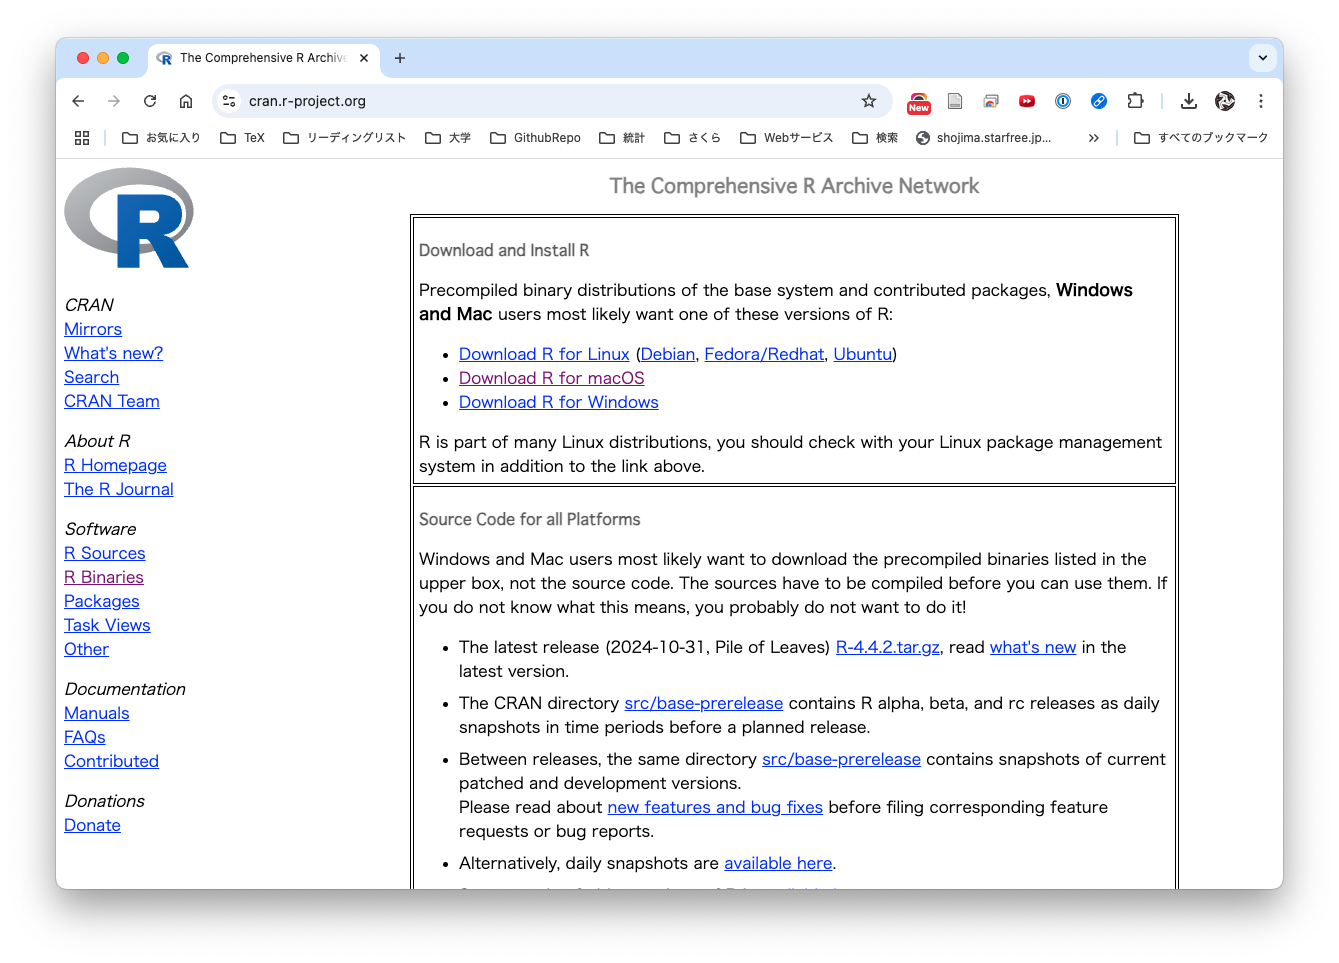
\includegraphics[keepaspectratio]{cran.png}}

}

\caption{cranのページ}

\end{figure}%

\subsection{RStudioも使いましょう}\label{rstudioux3082ux4f7fux3044ux307eux3057ux3087ux3046}

\begin{enumerate}
\def\labelenumi{\arabic{enumi}.}
\tightlist
\item
  \texttt{RStudio}で検索します。\texttt{RStudio\ Desktop}あるいはPosit社が出てきます。
\item
  \texttt{Install\ RStudio}からRStudio
  Desktopをダウンロードしてインストールしましょう。
\end{enumerate}

RStudioはServer版もあります。サーバを用意すればブラウザ経由で簡単に使える利点があります。

\pandocbounded{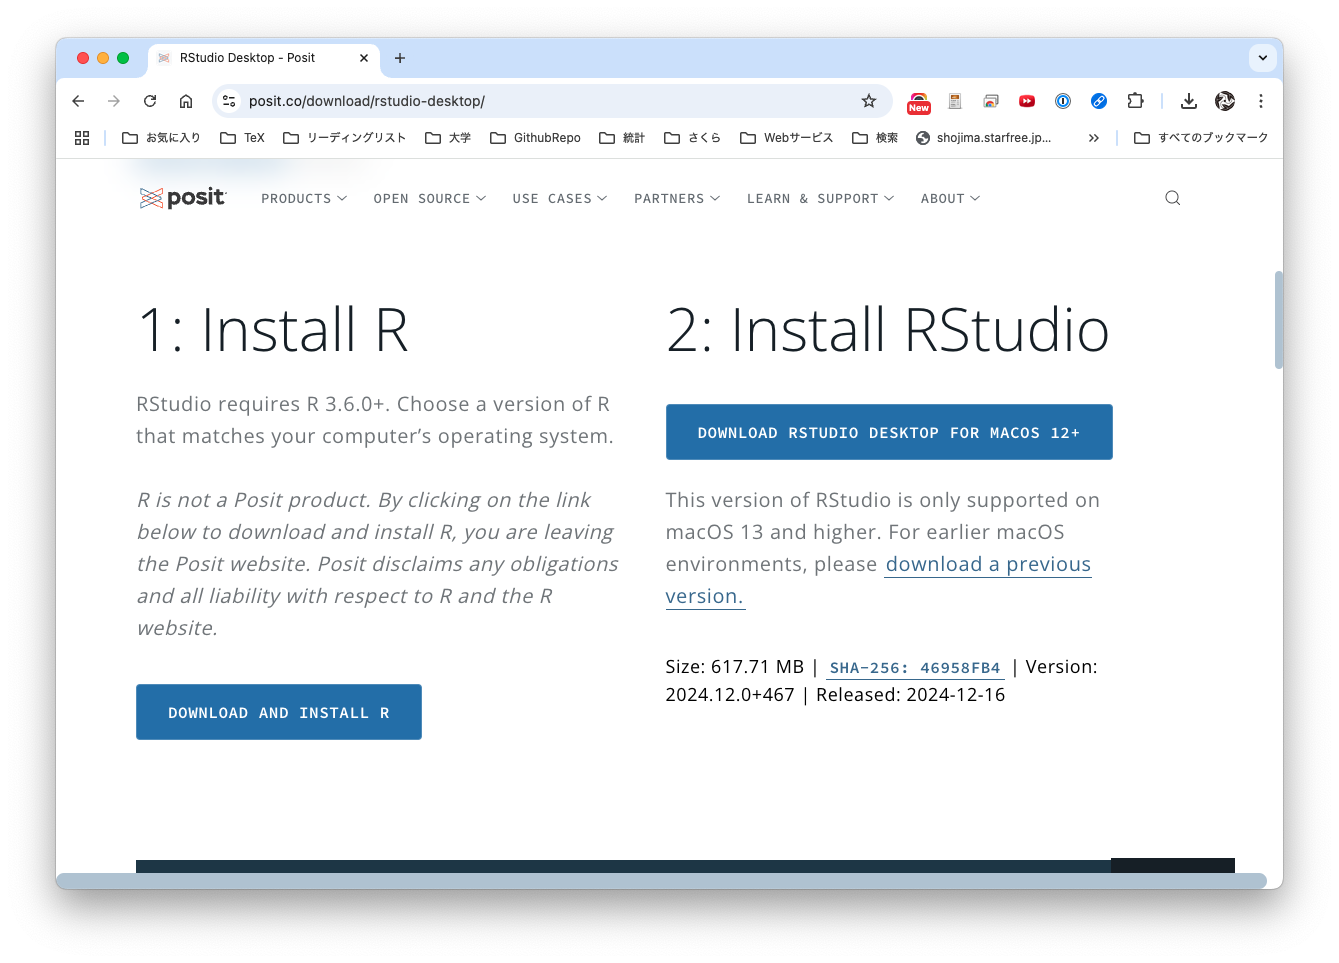
\includegraphics[keepaspectratio]{RStudio.png}}

\subsection{RStudioの起動画面}\label{rstudioux306eux8d77ux52d5ux753bux9762}

\begin{figure}[H]

{\centering \pandocbounded{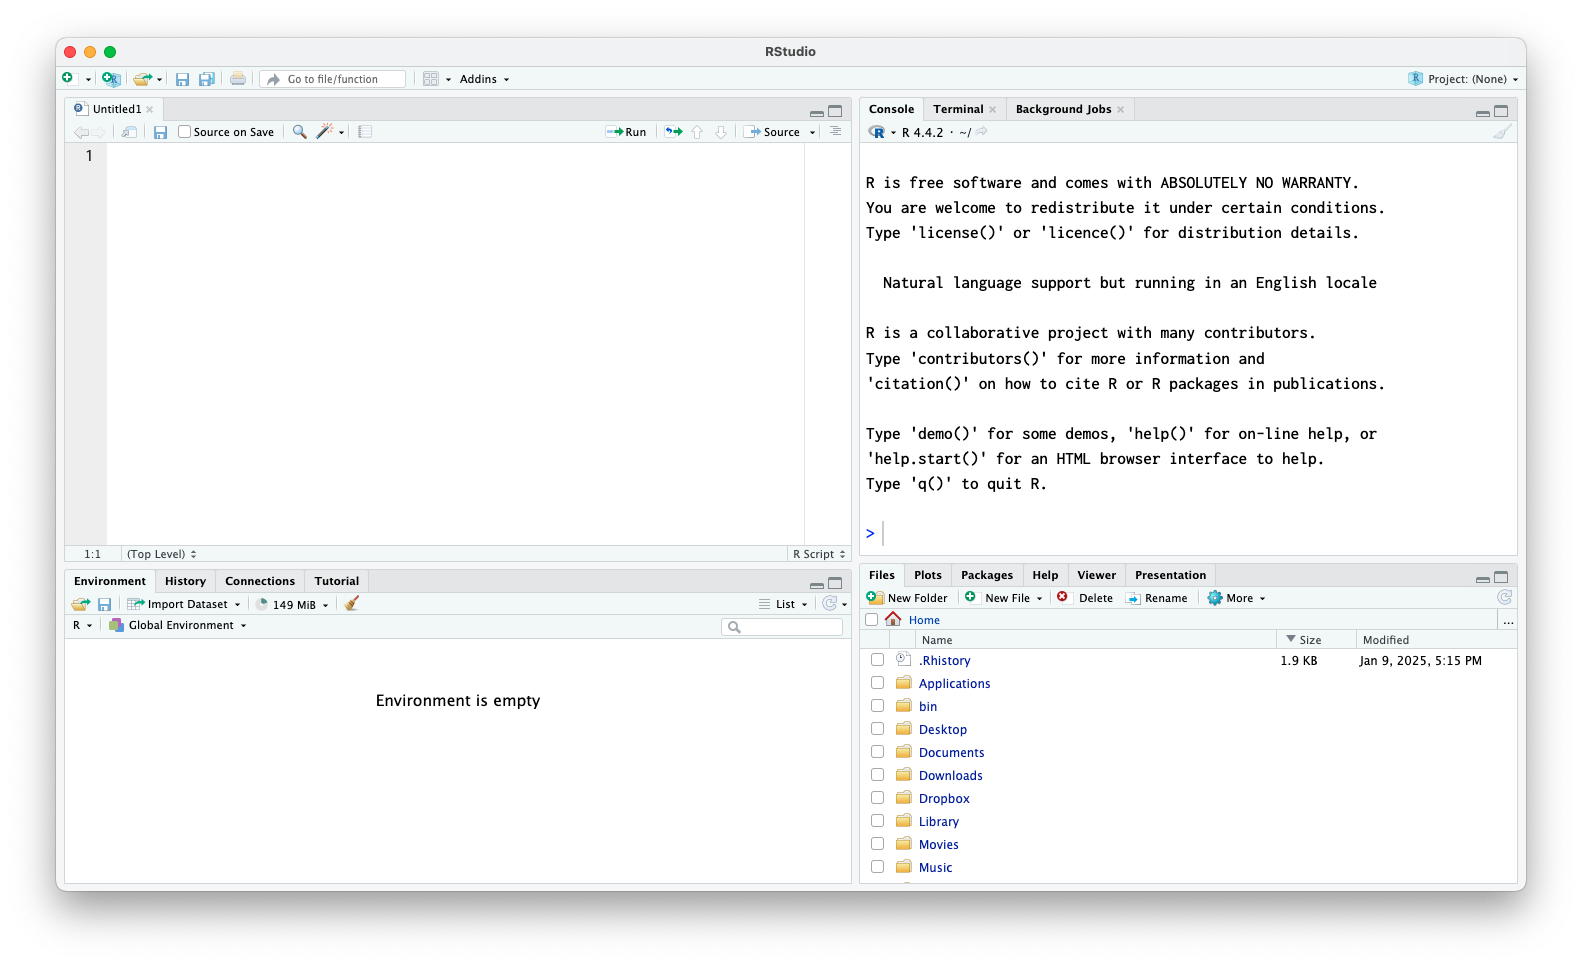
\includegraphics[keepaspectratio]{RStudioStartup.png}}

}

\caption{RStudi起動画面}

\end{figure}%

\begin{itemize}
\tightlist
\item
  大きく4分割して使います。
\item
  起動して最初にやるのが「\textbf{環境設定}」です。
\item
  メニューバーから,Tools \textgreater{} Global Optionsと進みます。
\end{itemize}

\subsection{オススメ設定}\label{ux30aaux30b9ux30b9ux30e1ux8a2dux5b9a}

\begin{figure}[H]

{\centering \pandocbounded{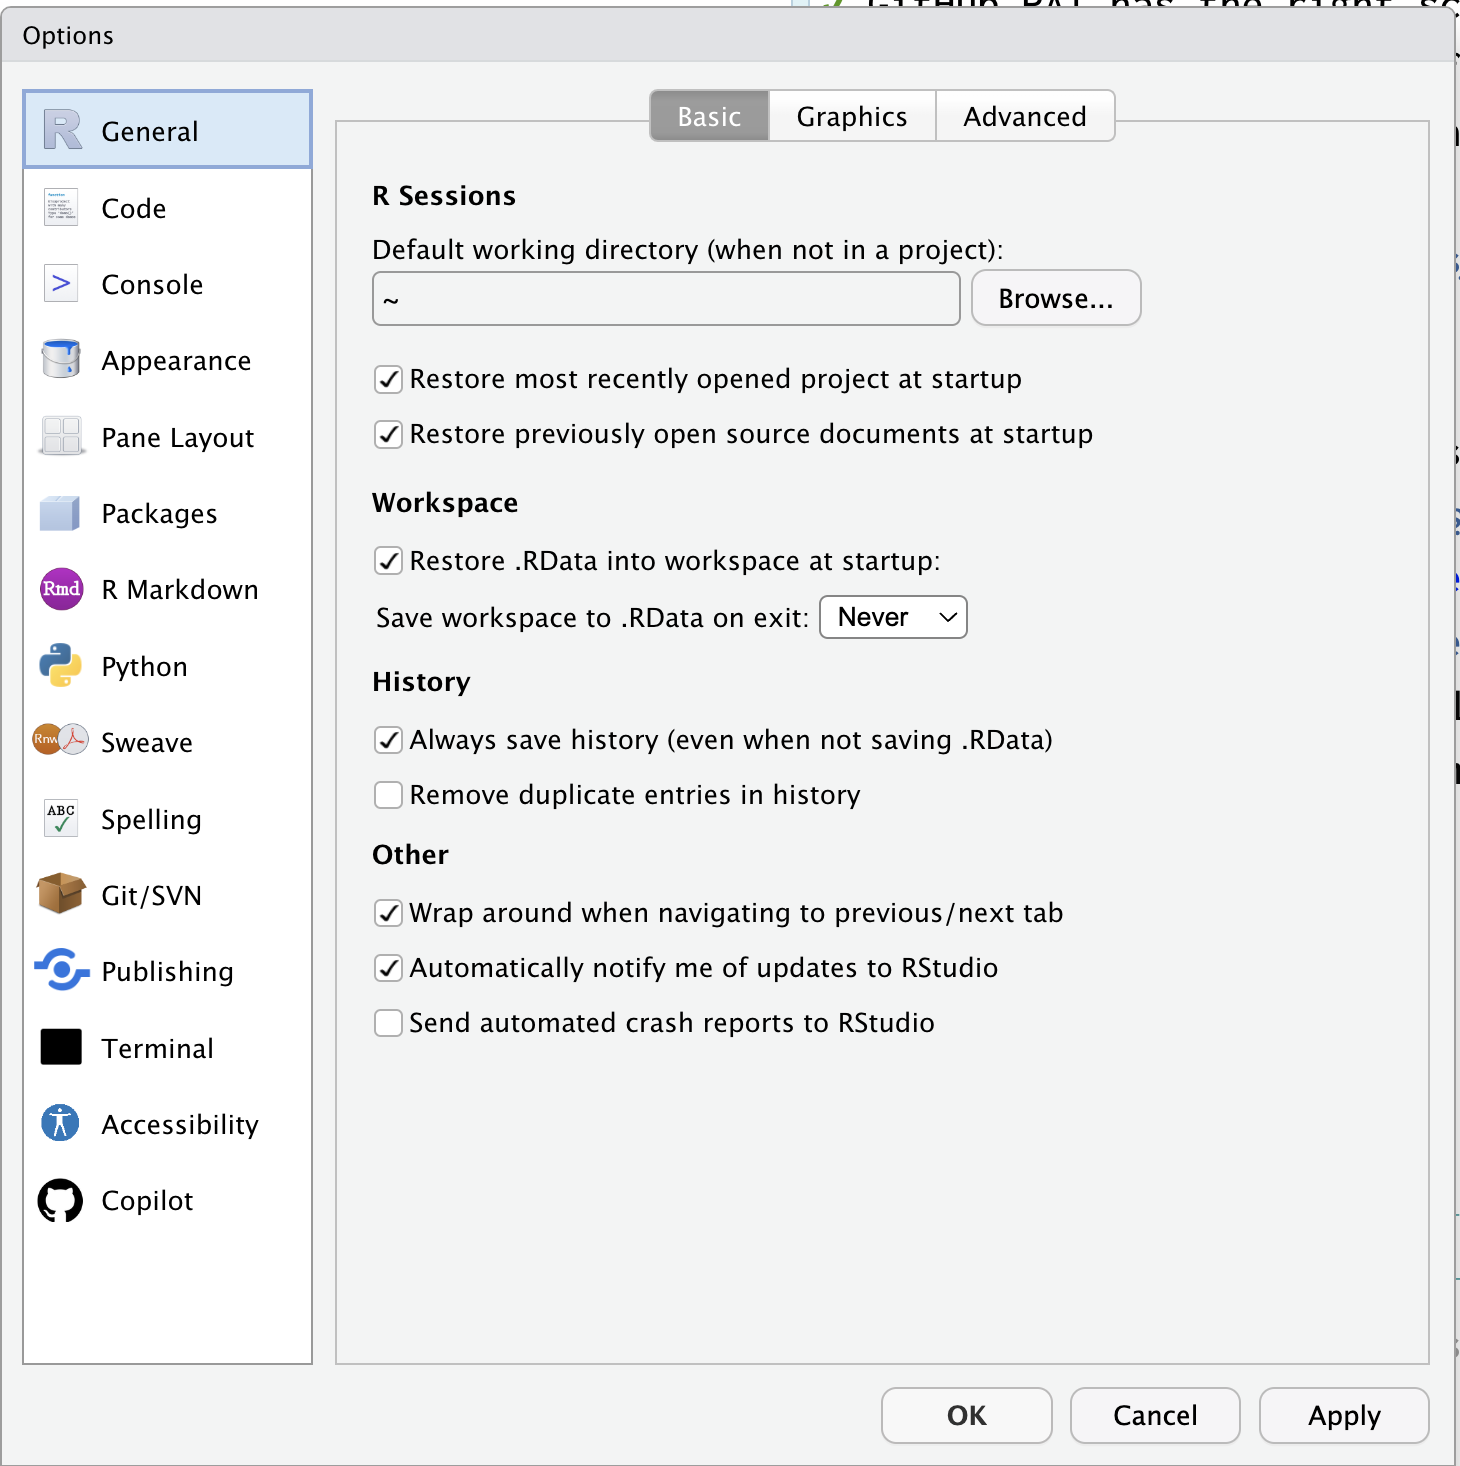
\includegraphics[keepaspectratio]{RStudioGlobalOptions.png}}

}

\caption{環境設定画面}

\end{figure}%

\begin{itemize}
\tightlist
\item
  General \textgreater{} Basic
  のWrokspace,\texttt{Save\ Workspace\ to\ .RData\ on\ exit:}を\textbf{never}に
\item
  General \textgreater{} Graphics \textgreater{} Graphics
  Deviceの\texttt{Backend}を\textbf{AGG}に
\item
  Appearance の \texttt{Editor\ Font}を見やすいフォントにしましょう
\item
  Appearance の \texttt{Editor\ Font\ size}を見やすい大きさにしましょう
\end{itemize}

おすすめフォント

\begin{itemize}
\tightlist
\item
  \href{https://github.com/yuru7/bizin-gothic}{Bizin Gothic}
\item
  \href{https://github.com/yuru7/HackGen}{HackGen}
\end{itemize}

\subsection{オススメ設定(つづき)}\label{ux30aaux30b9ux30b9ux30e1ux8a2dux5b9aux3064ux3065ux304d}

\begin{figure}[H]

{\centering \pandocbounded{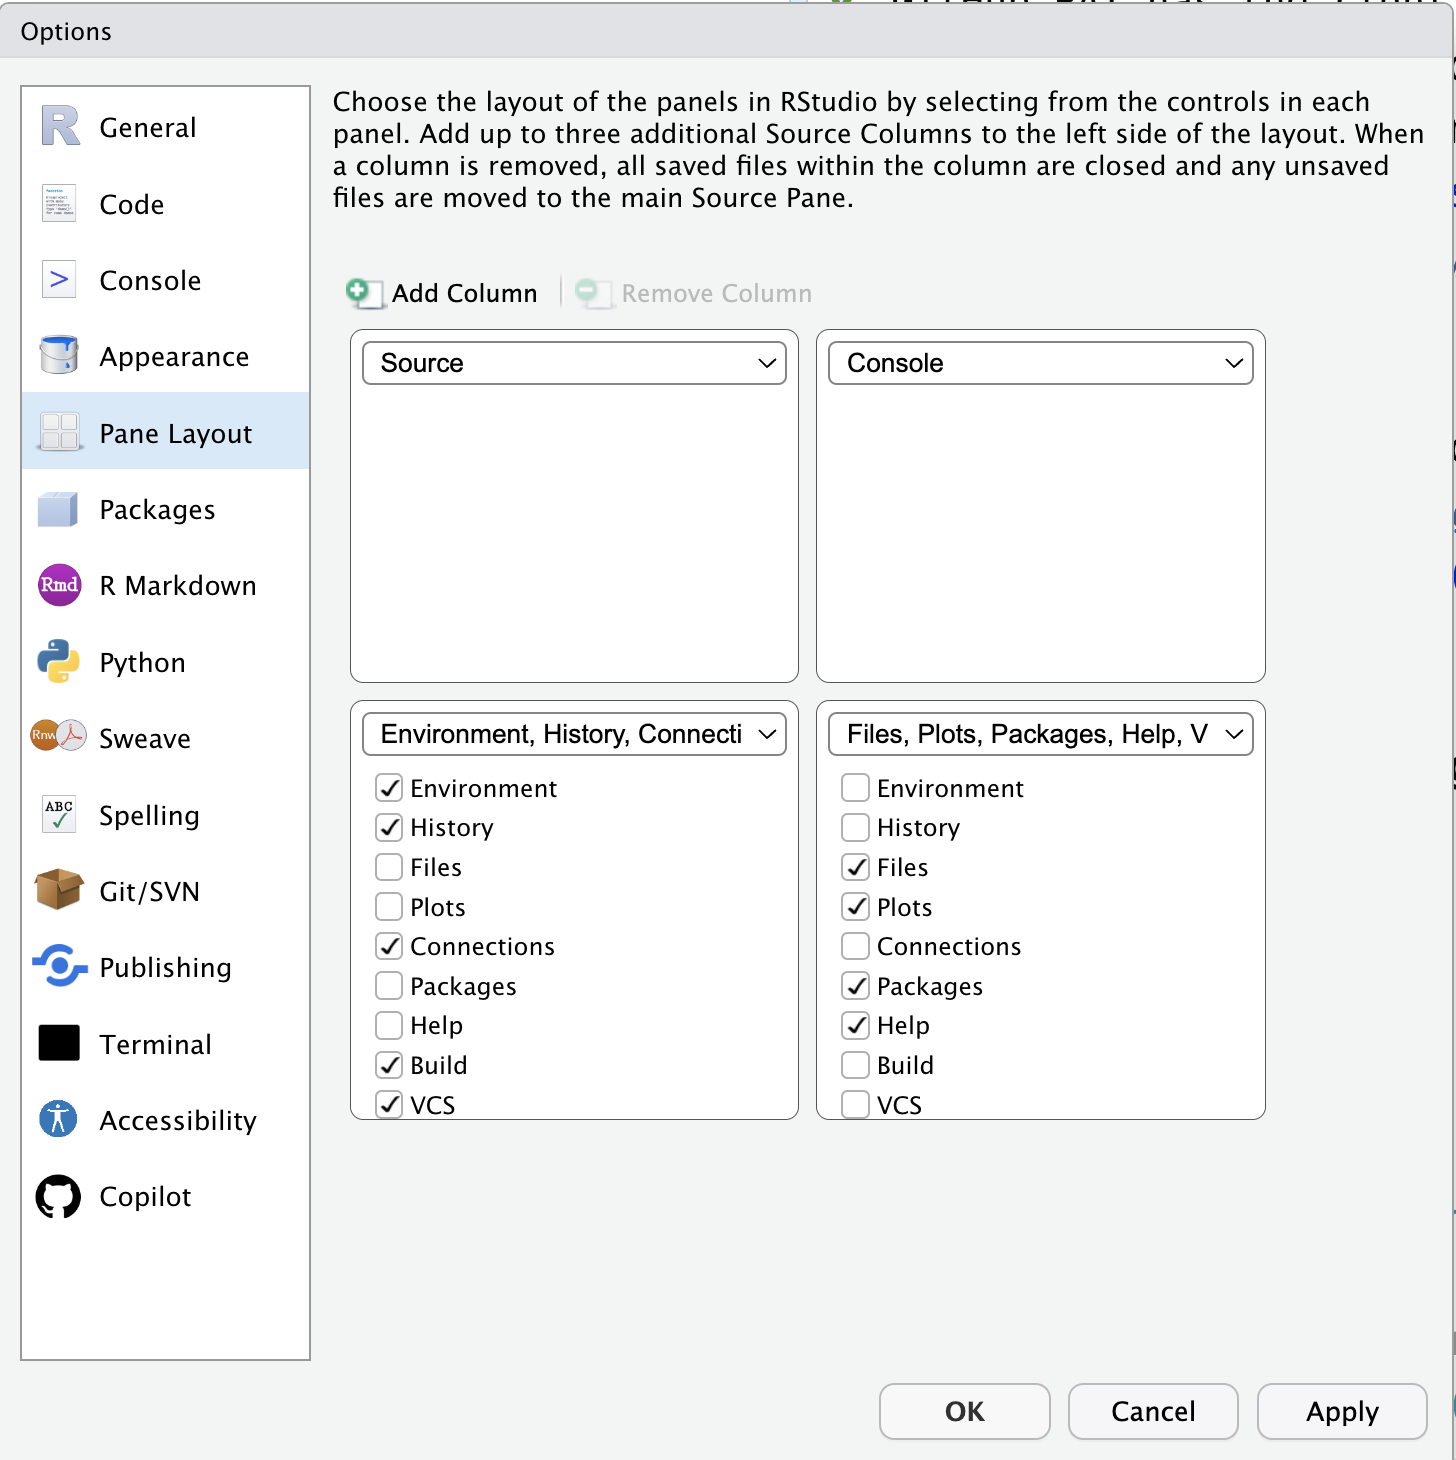
\includegraphics[keepaspectratio]{RStudioPaneLayout.png}}

}

\caption{環境設定画面その2}

\end{figure}%

\begin{itemize}
\tightlist
\item
  Pane Layoutを

  \begin{itemize}
  \tightlist
  \item
    \textbf{Source}と\textbf{Cosole}を横並びに
  \item
    かなりワイドな画面をお使いの方は,\texttt{Add\ Column}で3列にしてsource
    paneを一列増やそう
  \end{itemize}
\item
  設定が終わったら \textbf{Apply(適用)} ボタンをおして,\textbf{OK}
  で閉じる
\end{itemize}

\subsection{RStudioの4つの窓}\label{rstudioux306e4ux3064ux306eux7a93}

\begin{figure}[H]

{\centering \pandocbounded{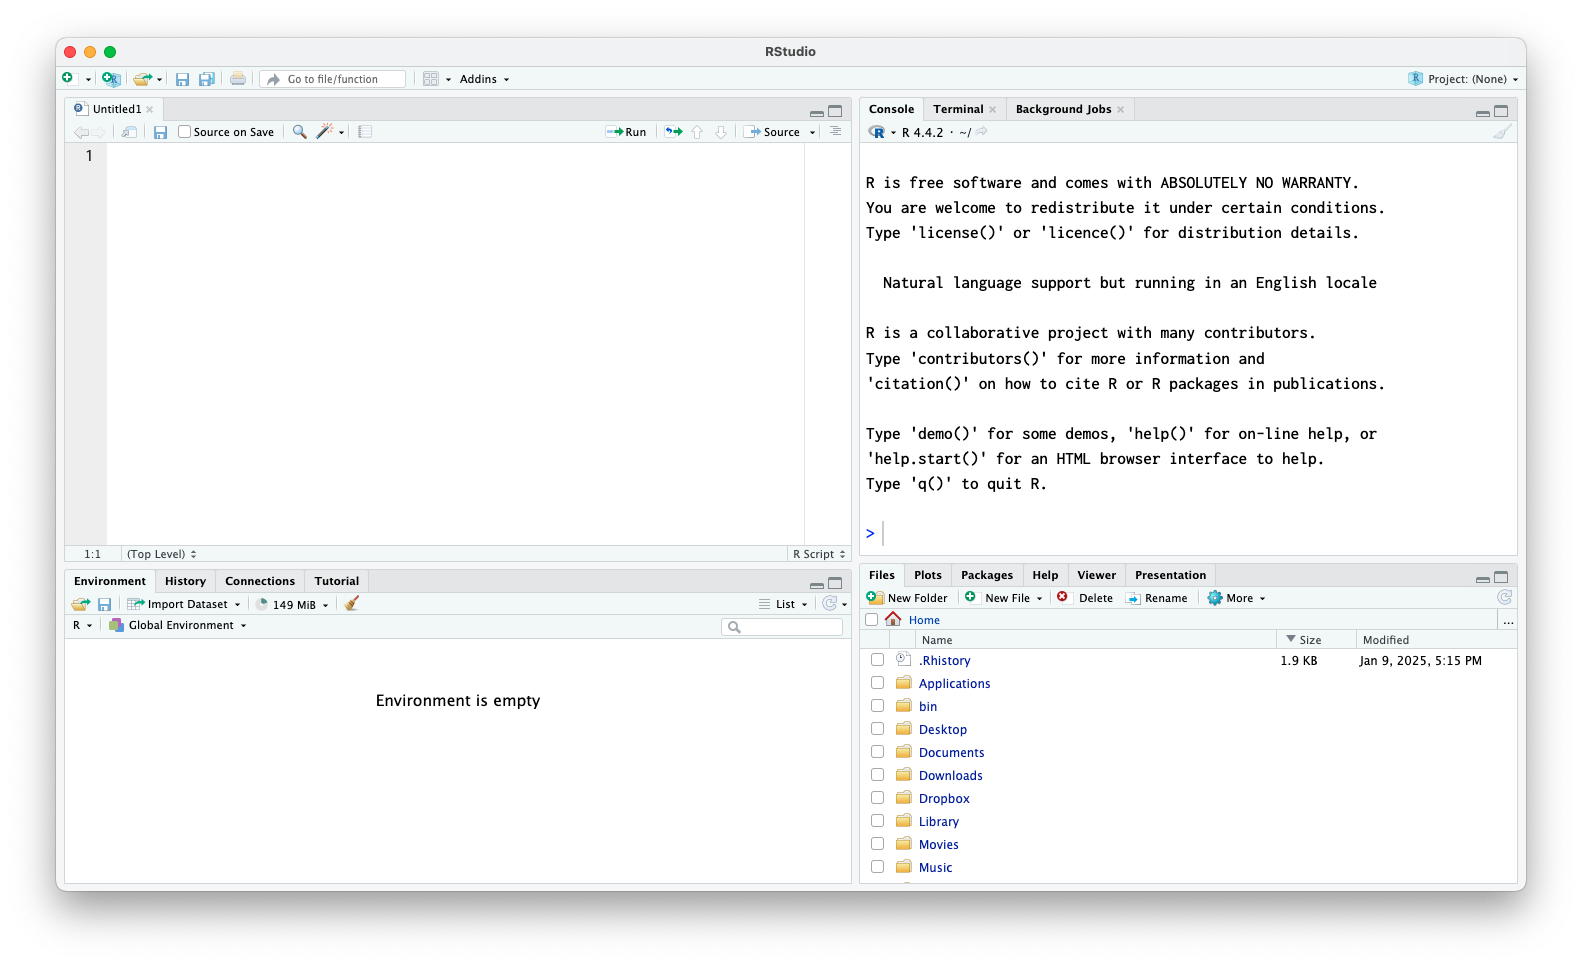
\includegraphics[keepaspectratio]{RStudioStartup.png}}

}

\caption{4つのペイン}

\end{figure}%

\begin{itemize}
\tightlist
\item
  \texttt{Source}ペインはエディタ領域で,Rスクリプトを書く場所。
\item
  \texttt{Console}ペインはRエンジン。直接Rコードを書いてもいいし,\texttt{Source}から一行ずつ,あるいは\texttt{Source}全体を流し込んで計算を実行する。
\end{itemize}

\subsection{RStudioの4つの窓}\label{rstudioux306e4ux3064ux306eux7a93-1}

\begin{figure}[H]

{\centering \pandocbounded{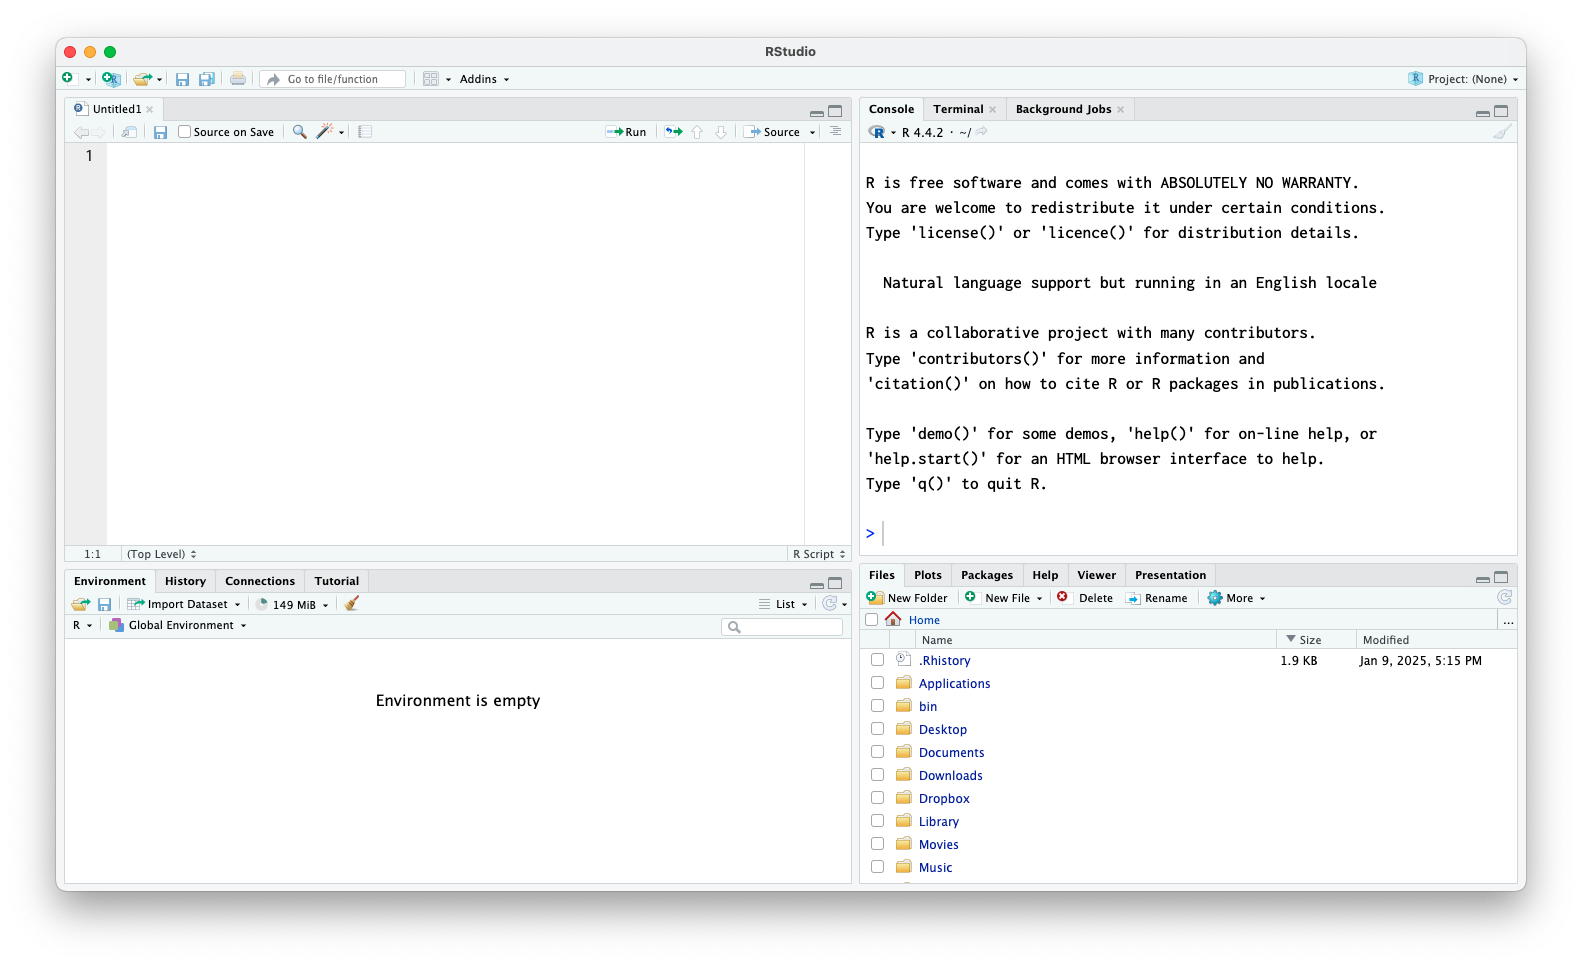
\includegraphics[keepaspectratio]{RStudioStartup.png}}

}

\caption{ペインの確認1}

\end{figure}%

\begin{itemize}
\tightlist
\item
  \texttt{Environment}はメモリに入っている変数・オブジェクトを表示
\item
  \texttt{Files}はワーキングディレクトリの表示,簡単な操作
\item
  \texttt{Package}はパッケージ管理(後述)
\item
  \texttt{Plots},\texttt{Viewer}は出力表示
\end{itemize}

\subsection{Rはプロジェクト管理が基本}\label{rux306fux30d7ux30edux30b8ux30a7ux30afux30c8ux7ba1ux7406ux304cux57faux672c}

\begin{itemize}
\tightlist
\item
  プロジェクト=フォルダに紐づいた作業環境を作ろう

  \begin{itemize}
  \tightlist
  \item
    File \textgreater{} New ProjectからNew Directory/Existing
    Directory/Version Controlを選ぶ

    \begin{itemize}
    \tightlist
    \item
      New Directory; 新しいフォルダで作業開始
    \item
      Existing Directory; 既存のフォルダをプロジェクトと紐付け
    \item
      Version Control; Githubレポジトリとプロジェクトを紐付け
    \end{itemize}
  \end{itemize}
\end{itemize}

プロジェクトにしておくと,作業フォルダの設定も自動でなされるから,ファイルの読み込みなどでパスの指定が楽になります。

\begin{itemize}
\tightlist
\item
  今回の春セミ用にプロジェクトフォルダを作りましょう!

  \begin{itemize}
  \tightlist
  \item
    すでにフォルダに色々まとめている人は,Existing Directoryから
  \item
    まだフォルダがない人は,New Directoryから
  \end{itemize}
\end{itemize}

\section{Rをさわってみましょう}\label{rux3092ux3055ux308fux3063ux3066ux307fux307eux3057ux3087ux3046}

\subsection{はじめの1歩}\label{ux306fux3058ux3081ux306e1ux6b69}

\begin{itemize}
\tightlist
\item
  Rはインタプリタ言語=一問一答

  \begin{itemize}
  \tightlist
  \item
    Consoleに\texttt{\textgreater{}}が出ていたら聞く準備ができています。
  \item
    Consoleに\texttt{+}が出ていたら前の入力が終わってません。
  \end{itemize}
\item
  直接Consoleに書き込むのではなく,スクリプトに書きましょう。

  \begin{itemize}
  \tightlist
  \item
    File \textgreater{} New File \textgreater{} R Script
    と進むと無名のスクリプトファイルが開きます
  \end{itemize}
\item
  スクリプトファイルが開いたら,まず次のように書きます。
\end{itemize}

\begin{Shaded}
\begin{Highlighting}[]
\FunctionTok{rm}\NormalTok{(}\AttributeTok{list =} \FunctionTok{ls}\NormalTok{())}
\end{Highlighting}
\end{Shaded}

\begin{itemize}
\tightlist
\item
  一行目は呪文のようなものだと思ってください。

  \begin{itemize}
  \tightlist
  \item
    \texttt{rm}という関数はremoveを意味していて,現在Rのメモリにある変数やオブジェクトを除外します。
  \item
    \texttt{list=ls()}は「メモリのすべてのオブジェクトリスト」を意味するので,これで環境の初期化になります。
  \end{itemize}
\end{itemize}

\subsection{パッケージ}\label{ux30d1ux30c3ux30b1ux30fcux30b8}

\begin{itemize}
\tightlist
\item
  パッケージは関数のセット。元のRに追加するだけで機能が増えます。
\item
  パッケージはCRANを通じて公開され,ペインの\texttt{Packages}タブで管理できます。
\end{itemize}

\pandocbounded{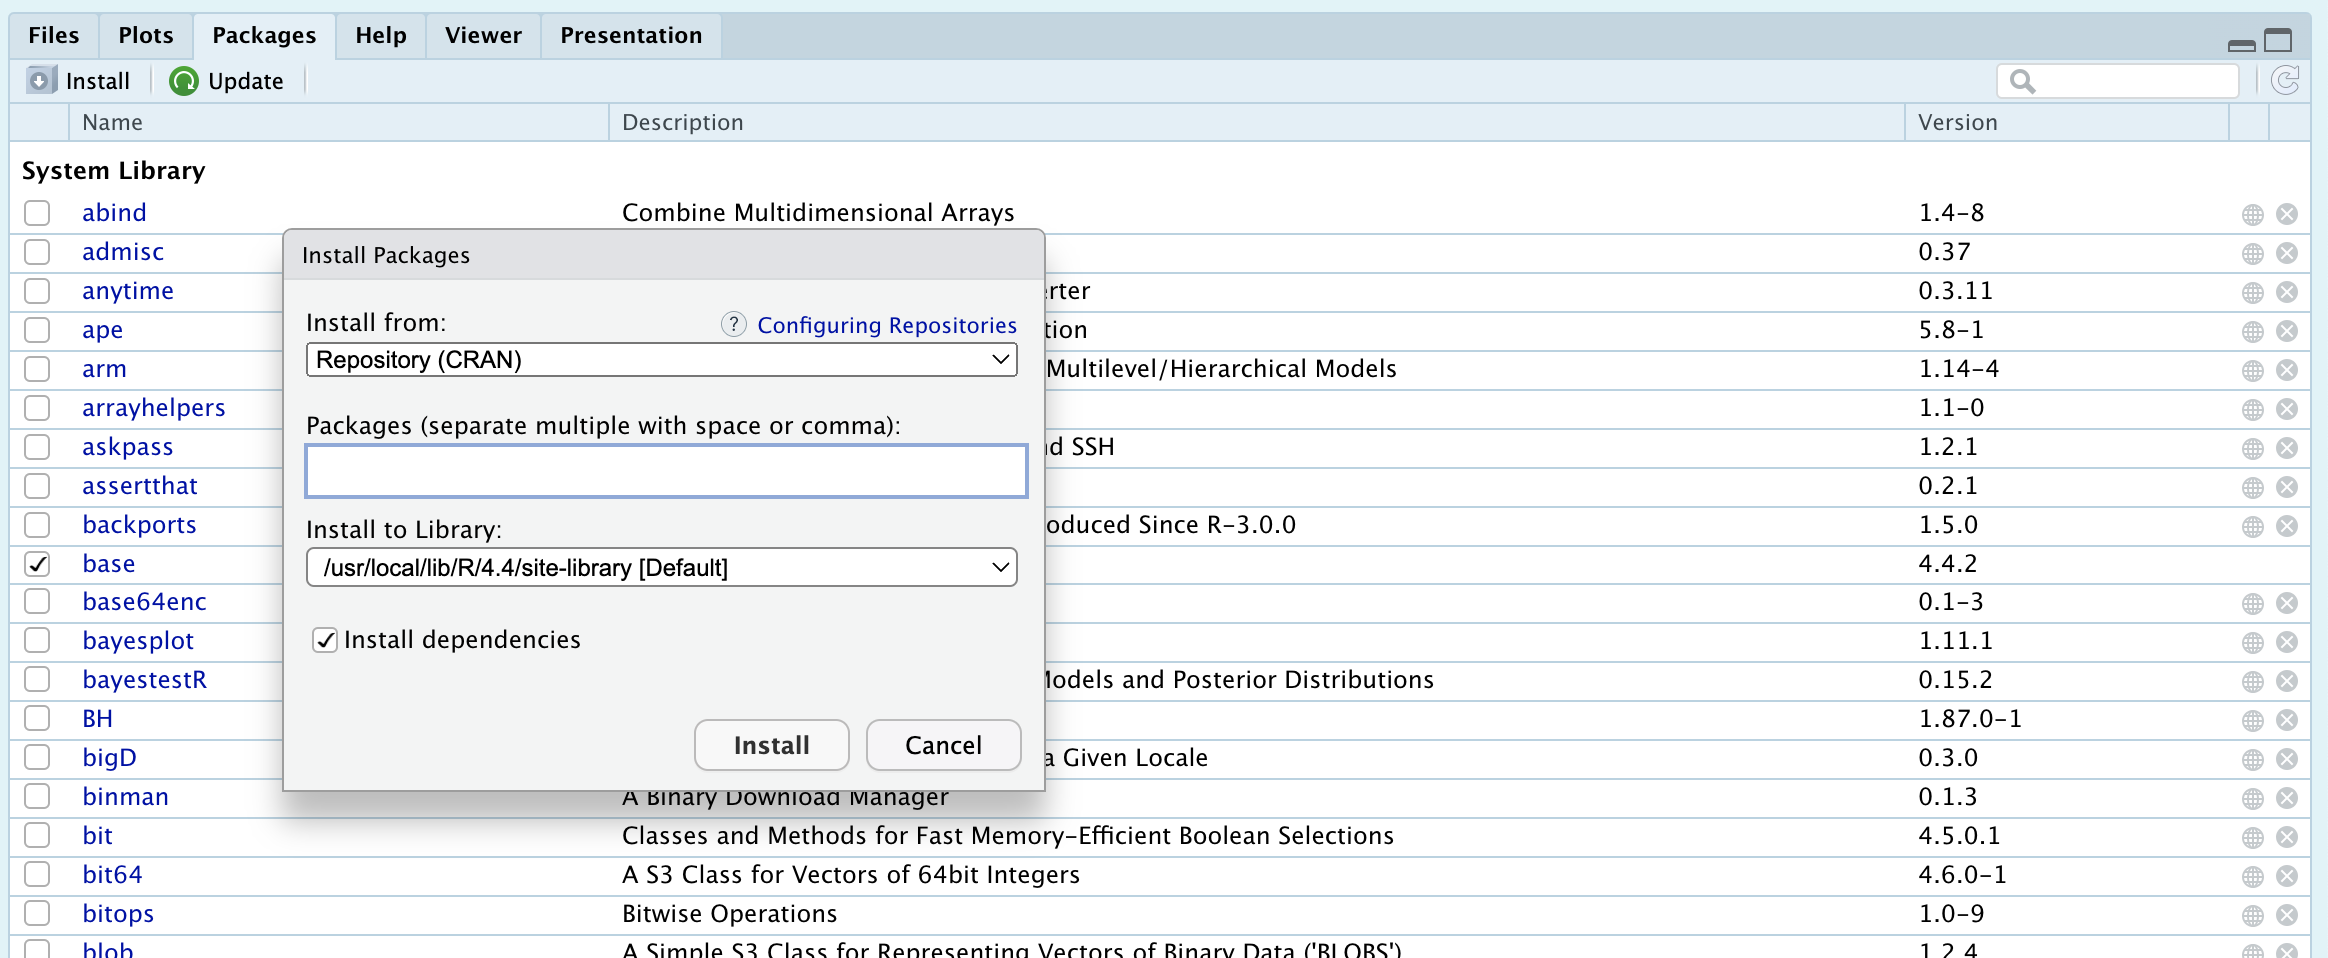
\includegraphics[keepaspectratio]{packages_tab.png}}

\begin{itemize}
\tightlist
\item
  デフォルトではCRANから取ってくることになります。(要ネット環境)

  \begin{itemize}
  \tightlist
  \item
    Packagesのところで\texttt{exametrika}と入力してインストールしちゃいましょう。
  \item
    あるパッケージが他のパッケージを必要とすることもあります。これを\textbf{依存パッケージ}といいます。
  \item
    RStudioのPackagesタブでは\texttt{install\ dependencies}にチェックがあるのがデフォルトです。

    \begin{itemize}
    \tightlist
    \item
      依存パッケージがあれば自動的にインストールされます。
    \item
      \texttt{exametrika}は\texttt{igraph}などに依存していますので,それらが同時に導入されます
    \end{itemize}
  \end{itemize}
\end{itemize}

\subsection{パッケージの使い方}\label{ux30d1ux30c3ux30b1ux30fcux30b8ux306eux4f7fux3044ux65b9}

\begin{itemize}
\tightlist
\item
  パッケージを使うには\texttt{library}と書きます。
\end{itemize}

\begin{Shaded}
\begin{Highlighting}[]
\FunctionTok{library}\NormalTok{(exametrika)}
\end{Highlighting}
\end{Shaded}

\begin{verbatim}
Loading required package: mvtnorm
\end{verbatim}

\begin{verbatim}
Loading required package: igraph
\end{verbatim}

\begin{verbatim}

Attaching package: 'igraph'
\end{verbatim}

\begin{verbatim}
The following objects are masked from 'package:stats':

    decompose, spectrum
\end{verbatim}

\begin{verbatim}
The following object is masked from 'package:base':

    union
\end{verbatim}

\begin{itemize}
\item
  これで\texttt{exametrika}パッケージの持つ関数が実行できるようになりました!他のパッケージも同様です。
\item
  パッケージのインストールを毎回する必要はありません。インストールは「手に入れる」ということだからです。
\item
  パッケージの実装(\texttt{library})はセッション毎に行う必要があります。これは「そうびする」ようなものです。
\item
  Rスクリプトの冒頭で\texttt{rm(list=ls())}としましたが,分析に必要なパッケージはスクリプトの最上部にまとめて書いておきましょう。

  \begin{itemize}
  \tightlist
  \item
    Rはインタプリタなので,逐次的に処理が進みますが,行ったり来たりしていると「パッケージを読み込んだっけ?」とか「今は何の数字で何の計算をしてるんだっけ?」となってしまいます。
  \item
    細かいことですが,パッケージは読み込む順番に影響されることがあります。

    \begin{itemize}
    \tightlist
    \item
      同じ関数名を異なるパッケージが使っている場合,後で読み込まれた方が上書きされます。
    \item
      混同しないように\texttt{PackageName::function}のように\texttt{::}で明示することがあります。
    \end{itemize}
  \end{itemize}
\end{itemize}

\subsection{数値計算の基礎}\label{ux6570ux5024ux8a08ux7b97ux306eux57faux790e}

\begin{itemize}
\tightlist
\item
  スクリプトに四則演算を書いて,Cmd+Enterでコンソールに送ります。
\item
  複数行選択/Runボタン/Sourceボタンをつかってもいいでしょう。
\end{itemize}

\begin{Shaded}
\begin{Highlighting}[]
\DecValTok{1} \SpecialCharTok{+} \DecValTok{2}
\end{Highlighting}
\end{Shaded}

\begin{verbatim}
[1] 3
\end{verbatim}

\begin{Shaded}
\begin{Highlighting}[]
\DecValTok{3} \SpecialCharTok{{-}} \DecValTok{4}
\end{Highlighting}
\end{Shaded}

\begin{verbatim}
[1] -1
\end{verbatim}

\begin{Shaded}
\begin{Highlighting}[]
\DecValTok{5} \SpecialCharTok{*} \DecValTok{6}
\end{Highlighting}
\end{Shaded}

\begin{verbatim}
[1] 30
\end{verbatim}

\begin{Shaded}
\begin{Highlighting}[]
\DecValTok{7} \SpecialCharTok{/} \DecValTok{3}
\end{Highlighting}
\end{Shaded}

\begin{verbatim}
[1] 2.333333
\end{verbatim}

\begin{itemize}
\tightlist
\item
  出力に\texttt{{[}1{]}}とあるのは気にしないでください。

  \begin{itemize}
  \tightlist
  \item
    Rはベクトルで処理します。今回の演算も,要素が1つのベクトルとして考えて処理しています。
  \end{itemize}
\end{itemize}

\subsection{数値計算の基礎}\label{ux6570ux5024ux8a08ux7b97ux306eux57faux790e-1}

\begin{itemize}
\tightlist
\item
  計算結果を保持する,あるいは名前をつけて管理することができます。
\item
  Rは「名前をつけて管理する対象」をすべて\textbf{オブジェクト}といいます。
\end{itemize}

\begin{Shaded}
\begin{Highlighting}[]
\NormalTok{a }\OtherTok{\textless{}{-}} \DecValTok{1} \SpecialCharTok{+} \DecValTok{2}
\NormalTok{b }\OtherTok{\textless{}{-}} \DecValTok{3} \SpecialCharTok{{-}} \DecValTok{4}
\FunctionTok{print}\NormalTok{(a)}
\end{Highlighting}
\end{Shaded}

\begin{verbatim}
[1] 3
\end{verbatim}

\begin{Shaded}
\begin{Highlighting}[]
\FunctionTok{print}\NormalTok{(b)}
\end{Highlighting}
\end{Shaded}

\begin{verbatim}
[1] -1
\end{verbatim}

\begin{Shaded}
\begin{Highlighting}[]
\FunctionTok{print}\NormalTok{(a }\SpecialCharTok{+}\NormalTok{ b)}
\end{Highlighting}
\end{Shaded}

\begin{verbatim}
[1] 2
\end{verbatim}

\begin{itemize}
\tightlist
\item
  \texttt{\textless{}-}で代入を意味します。ショートカット(ALTと-,optionと-)も覚えておこう
\item
  RStudioの\texttt{Environment}タブに保存されているオブジェクトが表示されています。ダブルクリックで確認できます。
\end{itemize}

\begin{Shaded}
\begin{Highlighting}[]
\NormalTok{a }\OtherTok{\textless{}{-}} \DecValTok{5}
\NormalTok{a }\SpecialCharTok{+}\NormalTok{ b}
\end{Highlighting}
\end{Shaded}

\begin{verbatim}
[1] 4
\end{verbatim}

同じオブジェクト名なら上書きされることに注意

\subsection{ベクトル,行列,リスト,データフレーム}\label{ux30d9ux30afux30c8ux30ebux884cux5217ux30eaux30b9ux30c8ux30c7ux30fcux30bfux30d5ux30ecux30fcux30e0}

\begin{itemize}
\tightlist
\item
  複数の数字のセット,\textbf{ベクトル}は\texttt{c()}でくくることで表現します。

  \begin{itemize}
  \tightlist
  \item
    連続した数字はコロン\texttt{:}で表現します。
  \end{itemize}
\item
  2次元に並ぶ数字のセット,\textbf{行列}は\texttt{matrix()}でつくります。

  \begin{itemize}
  \tightlist
  \item
    \texttt{matrix}関数にベクトルを与えるなどします。
  \end{itemize}
\item
  3次元以上の数字のセット,\textbf{配列}は\texttt{array()}で,\texttt{dim}オプションで各次元の大きさを指定します。
\item
  数字,文字,論理値(T/F)などが混在するもののセット,\textbf{リスト}は\texttt{list()}でつくります。
\item
  リストの中でも矩形に整っている\textbf{データフレーム}は,\texttt{data.frame()}でつくります。
\end{itemize}

分析するときはデータフレームがもっともよく使われます

データフレームの上位互換,\texttt{tibble}という型もあります。これは\texttt{tibble}パッケージを読み込むことで使えるようになります。

\subsection{ベクトル(Vector)の例}\label{ux30d9ux30afux30c8ux30ebvectorux306eux4f8b}

\subsubsection{数値ベクトル}\label{ux6570ux5024ux30d9ux30afux30c8ux30eb}

\begin{Shaded}
\begin{Highlighting}[]
\NormalTok{x }\OtherTok{\textless{}{-}} \FunctionTok{c}\NormalTok{(}\DecValTok{1}\NormalTok{, }\DecValTok{2}\NormalTok{, }\DecValTok{3}\NormalTok{, }\DecValTok{4}\NormalTok{, }\DecValTok{5}\NormalTok{)}
\FunctionTok{print}\NormalTok{(x)}
\end{Highlighting}
\end{Shaded}

\begin{verbatim}
[1] 1 2 3 4 5
\end{verbatim}

\subsubsection{文字列ベクトル}\label{ux6587ux5b57ux5217ux30d9ux30afux30c8ux30eb}

\begin{Shaded}
\begin{Highlighting}[]
\NormalTok{y }\OtherTok{\textless{}{-}} \FunctionTok{c}\NormalTok{(}\StringTok{"りんご"}\NormalTok{, }\StringTok{"みかん"}\NormalTok{, }\StringTok{"バナナ"}\NormalTok{)}
\FunctionTok{print}\NormalTok{(y)}
\end{Highlighting}
\end{Shaded}

\begin{verbatim}
[1] "りんご" "みかん" "バナナ"
\end{verbatim}

\subsubsection{論理値ベクトル}\label{ux8ad6ux7406ux5024ux30d9ux30afux30c8ux30eb}

\begin{itemize}
\tightlist
\item
  Rには文字,数字以外に論理値というのがあります。真/TRUEか偽/FALSEか,を表します。
\item
  使い方としては,論理判断の条件で使ったり,オプションの「スイッチオン・オフ」を表す時につかいます。
\item
  大文字の\texttt{T}や\texttt{F}は論理値を表す特別な用語(予約語)です。
\end{itemize}

\begin{Shaded}
\begin{Highlighting}[]
\NormalTok{z }\OtherTok{\textless{}{-}} \FunctionTok{c}\NormalTok{(}\ConstantTok{TRUE}\NormalTok{, }\ConstantTok{FALSE}\NormalTok{, }\ConstantTok{TRUE}\NormalTok{)}
\FunctionTok{print}\NormalTok{(z)}
\end{Highlighting}
\end{Shaded}

\begin{verbatim}
[1]  TRUE FALSE  TRUE
\end{verbatim}

\subsection{行列(Matrix)}\label{ux884cux5217matrix}

\begin{itemize}
\tightlist
\item
  1から9までの数字で3×3行列を作成
\end{itemize}

\begin{Shaded}
\begin{Highlighting}[]
\NormalTok{m1 }\OtherTok{\textless{}{-}} \FunctionTok{matrix}\NormalTok{(}\DecValTok{1}\SpecialCharTok{:}\DecValTok{9}\NormalTok{, }\AttributeTok{nrow =} \DecValTok{3}\NormalTok{, }\AttributeTok{ncol =} \DecValTok{3}\NormalTok{)}
\FunctionTok{print}\NormalTok{(m1)}
\end{Highlighting}
\end{Shaded}

\begin{verbatim}
     [,1] [,2] [,3]
[1,]    1    4    7
[2,]    2    5    8
[3,]    3    6    9
\end{verbatim}

\begin{itemize}
\tightlist
\item
  行名と列名を付ける
\end{itemize}

\begin{Shaded}
\begin{Highlighting}[]
\NormalTok{m2 }\OtherTok{\textless{}{-}} \FunctionTok{matrix}\NormalTok{(}\DecValTok{1}\SpecialCharTok{:}\DecValTok{9}\NormalTok{,}
    \AttributeTok{nrow =} \DecValTok{3}\NormalTok{, }\AttributeTok{ncol =} \DecValTok{3}\NormalTok{,}
    \AttributeTok{dimnames =} \FunctionTok{list}\NormalTok{(}
        \FunctionTok{c}\NormalTok{(}\StringTok{"A"}\NormalTok{, }\StringTok{"B"}\NormalTok{, }\StringTok{"C"}\NormalTok{),}
        \FunctionTok{c}\NormalTok{(}\StringTok{"X"}\NormalTok{, }\StringTok{"Y"}\NormalTok{, }\StringTok{"Z"}\NormalTok{)}
\NormalTok{    )}
\NormalTok{)}
\FunctionTok{print}\NormalTok{(m2)}
\end{Highlighting}
\end{Shaded}

\begin{verbatim}
  X Y Z
A 1 4 7
B 2 5 8
C 3 6 9
\end{verbatim}

\subsection{配列(Array)}\label{ux914dux5217array}

\begin{itemize}
\tightlist
\item
  2×3×2の3次元配列を作成
\end{itemize}

\begin{Shaded}
\begin{Highlighting}[]
\NormalTok{arr }\OtherTok{\textless{}{-}} \FunctionTok{array}\NormalTok{(}\DecValTok{1}\SpecialCharTok{:}\DecValTok{12}\NormalTok{, }\AttributeTok{dim =} \FunctionTok{c}\NormalTok{(}\DecValTok{2}\NormalTok{, }\DecValTok{3}\NormalTok{, }\DecValTok{2}\NormalTok{))}
\FunctionTok{print}\NormalTok{(arr)}
\end{Highlighting}
\end{Shaded}

\begin{verbatim}
, , 1

     [,1] [,2] [,3]
[1,]    1    3    5
[2,]    2    4    6

, , 2

     [,1] [,2] [,3]
[1,]    7    9   11
[2,]    8   10   12
\end{verbatim}

\subsection{リスト(List)}\label{ux30eaux30b9ux30c8list}

\begin{itemize}
\tightlist
\item
  様々な型のデータを含むリストを作成
\end{itemize}

\begin{Shaded}
\begin{Highlighting}[]
\NormalTok{my\_list }\OtherTok{\textless{}{-}} \FunctionTok{list}\NormalTok{(}
    \AttributeTok{numbers =} \FunctionTok{c}\NormalTok{(}\DecValTok{1}\NormalTok{, }\DecValTok{2}\NormalTok{, }\DecValTok{3}\NormalTok{),}
    \AttributeTok{text =} \StringTok{"Hello"}\NormalTok{,}
    \AttributeTok{logical =} \ConstantTok{TRUE}\NormalTok{,}
    \AttributeTok{matrix =} \FunctionTok{matrix}\NormalTok{(}\DecValTok{1}\SpecialCharTok{:}\DecValTok{4}\NormalTok{, }\DecValTok{2}\NormalTok{, }\DecValTok{2}\NormalTok{)}
\NormalTok{)}
\FunctionTok{print}\NormalTok{(my\_list)}
\end{Highlighting}
\end{Shaded}

\begin{verbatim}
$numbers
[1] 1 2 3

$text
[1] "Hello"

$logical
[1] TRUE

$matrix
     [,1] [,2]
[1,]    1    3
[2,]    2    4
\end{verbatim}

\subsection{リスト(List)}\label{ux30eaux30b9ux30c8list-1}

\begin{itemize}
\tightlist
\item
  リストの要素へのアクセス

  \begin{itemize}
  \tightlist
  \item
    名前付きリストなら\texttt{\$}マークで呼び出せます
  \end{itemize}
\end{itemize}

\begin{Shaded}
\begin{Highlighting}[]
\NormalTok{my\_list}\SpecialCharTok{$}\NormalTok{numbers}
\end{Highlighting}
\end{Shaded}

\begin{verbatim}
[1] 1 2 3
\end{verbatim}

\begin{Shaded}
\begin{Highlighting}[]
\NormalTok{my\_list}\SpecialCharTok{$}\NormalTok{numbers[}\DecValTok{3}\NormalTok{]}
\end{Highlighting}
\end{Shaded}

\begin{verbatim}
[1] 3
\end{verbatim}

\begin{Shaded}
\begin{Highlighting}[]
\NormalTok{my\_list}\SpecialCharTok{$}\NormalTok{matrix[, }\DecValTok{2}\NormalTok{]}
\end{Highlighting}
\end{Shaded}

\begin{verbatim}
[1] 3 4
\end{verbatim}

\begin{Shaded}
\begin{Highlighting}[]
\NormalTok{my\_list}\SpecialCharTok{$}\NormalTok{matrix}
\end{Highlighting}
\end{Shaded}

\begin{verbatim}
     [,1] [,2]
[1,]    1    3
[2,]    2    4
\end{verbatim}

\subsection{データフレーム(Data
Frame)}\label{ux30c7ux30fcux30bfux30d5ux30ecux30fcux30e0data-frame}

\begin{itemize}
\tightlist
\item
  データフレームの作成例

  \begin{itemize}
  \tightlist
  \item
    データフレームはリストの特殊な型なので,リストを\texttt{as.data.frame}関数で変換してもOK
  \end{itemize}
\end{itemize}

\begin{Shaded}
\begin{Highlighting}[]
\NormalTok{df }\OtherTok{\textless{}{-}} \FunctionTok{data.frame}\NormalTok{(}
    \AttributeTok{name =} \FunctionTok{c}\NormalTok{(}\StringTok{"田中"}\NormalTok{, }\StringTok{"鈴木"}\NormalTok{, }\StringTok{"佐藤"}\NormalTok{),}
    \AttributeTok{age =} \FunctionTok{c}\NormalTok{(}\DecValTok{25}\NormalTok{, }\DecValTok{30}\NormalTok{, }\DecValTok{28}\NormalTok{),}
    \AttributeTok{gender =} \FunctionTok{c}\NormalTok{(}\StringTok{"M"}\NormalTok{, }\StringTok{"F"}\NormalTok{, }\StringTok{"M"}\NormalTok{),}
    \AttributeTok{height =} \FunctionTok{c}\NormalTok{(}\DecValTok{170}\NormalTok{, }\DecValTok{160}\NormalTok{, }\DecValTok{175}\NormalTok{)}
\NormalTok{)}

\FunctionTok{print}\NormalTok{(df)}
\end{Highlighting}
\end{Shaded}

\begin{verbatim}
  name age gender height
1 田中  25      M    170
2 鈴木  30      F    160
3 佐藤  28      M    175
\end{verbatim}

\begin{itemize}
\tightlist
\item
  要素へのアクセスの仕方はリストと同じです
\end{itemize}

\begin{Shaded}
\begin{Highlighting}[]
\NormalTok{df}\SpecialCharTok{$}\NormalTok{age}
\end{Highlighting}
\end{Shaded}

\begin{verbatim}
[1] 25 30 28
\end{verbatim}

\subsection{データ構造の比較}\label{ux30c7ux30fcux30bfux69cbux9020ux306eux6bd4ux8f03}

\begin{longtable}[]{@{}
  >{\raggedright\arraybackslash}p{(\linewidth - 12\tabcolsep) * \real{0.1364}}
  >{\raggedright\arraybackslash}p{(\linewidth - 12\tabcolsep) * \real{0.2273}}
  >{\raggedright\arraybackslash}p{(\linewidth - 12\tabcolsep) * \real{0.1364}}
  >{\raggedright\arraybackslash}p{(\linewidth - 12\tabcolsep) * \real{0.1364}}
  >{\raggedright\arraybackslash}p{(\linewidth - 12\tabcolsep) * \real{0.1818}}
  >{\raggedright\arraybackslash}p{(\linewidth - 12\tabcolsep) * \real{0.0909}}
  >{\raggedright\arraybackslash}p{(\linewidth - 12\tabcolsep) * \real{0.0909}}@{}}
\toprule\noalign{}
\begin{minipage}[b]{\linewidth}\raggedright
特徴
\end{minipage} & \begin{minipage}[b]{\linewidth}\raggedright
ベクトル
\end{minipage} & \begin{minipage}[b]{\linewidth}\raggedright
行列
\end{minipage} & \begin{minipage}[b]{\linewidth}\raggedright
配列
\end{minipage} & \begin{minipage}[b]{\linewidth}\raggedright
リスト
\end{minipage} & \begin{minipage}[b]{\linewidth}\raggedright
df
\end{minipage} & \begin{minipage}[b]{\linewidth}\raggedright
Tibble
\end{minipage} \\
\midrule\noalign{}
\endhead
\bottomrule\noalign{}
\endlastfoot
次元 & 1次元 & 2次元 & n次元 & 階層構造 & 2次元 & 2次元 \\
型の統一 & 必要 & 必要 & 必要 & 不要 & 列ごと & 列ごと \\
データ型 & 単一 & 単一 & 単一 & 複数可 & 複数可 & 複数可 \\
主な用途 & 単純な数列 & 数値計算 & 多次元データ & 複雑なデータ &
データ分析 & データ分析 \\
\end{longtable}

tibble型はデータフレームの上位互換で,\texttt{tibble}パッケージを使うことで導入できます。主な特徴は次のとおりです。

\begin{itemize}
\tightlist
\item
  型情報の表示
\item
  行数と列数の表示
\item
  データの一部のみ表示(大きなデータセット時に便利)
\end{itemize}

\subsection{パイプ演算子を活用しよう}\label{ux30d1ux30a4ux30d7ux6f14ux7b97ux5b50ux3092ux6d3bux7528ux3057ux3088ux3046}

\begin{itemize}
\tightlist
\item
  パイプ演算子は、データの処理を順番に繋げてくれる記号
\item
  左から右へ、データが流れていくイメージ!コードが読みやすく、理解しやすくなる
\end{itemize}

\subsubsection{基本的な使い方}\label{ux57faux672cux7684ux306aux4f7fux3044ux65b9}

\begin{itemize}
\tightlist
\item
  パイプ演算子を使わないでいると?
\end{itemize}

\begin{Shaded}
\begin{Highlighting}[]
\NormalTok{result }\OtherTok{\textless{}{-}} \FunctionTok{sum}\NormalTok{(}\FunctionTok{sqrt}\NormalTok{(}\FunctionTok{abs}\NormalTok{(}\FunctionTok{log}\NormalTok{(}\FunctionTok{c}\NormalTok{(}\DecValTok{1}\SpecialCharTok{:}\DecValTok{10}\NormalTok{)))))}
\end{Highlighting}
\end{Shaded}

\begin{itemize}
\tightlist
\item
  パイプ演算子を使ってみると?
\end{itemize}

\begin{Shaded}
\begin{Highlighting}[]
\NormalTok{result }\OtherTok{\textless{}{-}} \FunctionTok{c}\NormalTok{(}\DecValTok{1}\SpecialCharTok{:}\DecValTok{10}\NormalTok{) }\SpecialCharTok{|\textgreater{}}
    \FunctionTok{log}\NormalTok{() }\SpecialCharTok{|\textgreater{}}
    \FunctionTok{abs}\NormalTok{() }\SpecialCharTok{|\textgreater{}}
    \FunctionTok{sqrt}\NormalTok{() }\SpecialCharTok{|\textgreater{}}
    \FunctionTok{sum}\NormalTok{()}
\end{Highlighting}
\end{Shaded}

\begin{itemize}
\tightlist
\item
  パイプ演算子はショートカット\texttt{Ctrl/Cmd\ +\ Shift\ +\ M}で入力できます

  \begin{itemize}
  \tightlist
  \item
    \texttt{\textbar{}\textgreater{}}はR4.1以降使えるようになった,Rのもってるパイプ演算子
  \item
    \texttt{\%\textgreater{}\%}は\texttt{magrittr}パッケージや,それを含んだ\texttt{tidyverse}パッケージで以前から使われていたもの
  \end{itemize}
\end{itemize}

\subsection{(余談)tidyな世界}\label{ux4f59ux8ac7tidyux306aux4e16ux754c}

\begin{itemize}
\tightlist
\item
  \texttt{tidyverse}パッケージは,データハンドリングを画期的に簡単にしたパッケージで,これでRのユーザが一気に広がったと言っても過言ではありません。
\item
  \texttt{tidyverse}パッケージはパッケージのパッケージ。

  \begin{itemize}
  \tightlist
  \item
    大規模データ用のデータフレーム,\texttt{tibble}
  \item
    パイプ演算子のパッケージ\texttt{magrittr}
  \item
    描画を綺麗にしてくれるパッケージ\texttt{ggplot2}などが含まれます
  \end{itemize}
\item
  専門の書籍も出ています
  \texttt{tidyverse}パッケージを基本にした\href{https://amzn.to/4bisTkc}{改訂2版RユーザのためのRStudio{[}実践{]}入門〜tidyverseによるモダンな分析フローの世界}
\end{itemize}

\subsection{(余談)チートシートを活用しよう}\label{ux4f59ux8ac7ux30c1ux30fcux30c8ux30b7ux30fcux30c8ux3092ux6d3bux7528ux3057ux3088ux3046}

\begin{itemize}
\tightlist
\item
  RStudioのメニューバー,Help\textgreater{} Cheat Sheetsと進んでください
\item
  PDFファイル1,2枚分で基本的な使い方を始めとした,様々なチートシートが現れます!
\end{itemize}

\pandocbounded{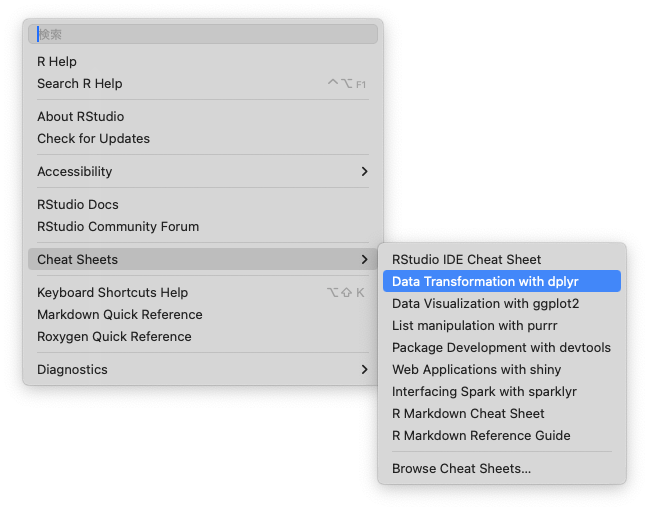
\includegraphics[keepaspectratio]{cheetSheet.png}}

\section{具体的にデータを扱ってみよう}\label{ux5177ux4f53ux7684ux306bux30c7ux30fcux30bfux3092ux6271ux3063ux3066ux307fux3088ux3046}

\subsection{データの読み込みと操作}\label{ux30c7ux30fcux30bfux306eux8aadux307fux8fbcux307fux3068ux64cdux4f5c}

\subsubsection{CSVファイルの読み込み}\label{csvux30d5ux30a1ux30a4ux30ebux306eux8aadux307fux8fbcux307f}

\begin{itemize}
\tightlist
\item
  CSVファイルはRでもっとも一般的なデータ形式の一つです
\item
  エクセルファイルなどと違って,アプリケーションに依存せず,メモ帳で開くこともできますので,あらゆるOSに対応できます。
\item
  基本的な読み込み方法は \texttt{read.csv()} 関数を使います
\item
  \texttt{tidyverse}パッケージを使っている人は,\texttt{read\_csv()}関数のほうが細かな調整が効いていいかも
\end{itemize}

\subsection{基本的なCSV読み込み}\label{ux57faux672cux7684ux306acsvux8aadux307fux8fbcux307f}

\begin{Shaded}
\begin{Highlighting}[]
\NormalTok{data }\OtherTok{\textless{}{-}} \FunctionTok{read.csv}\NormalTok{(}\StringTok{"data.csv"}\NormalTok{)}
\end{Highlighting}
\end{Shaded}

\subsubsection{日本語を含むCSVファイルの場合}\label{ux65e5ux672cux8a9eux3092ux542bux3080csvux30d5ux30a1ux30a4ux30ebux306eux5834ux5408}

\begin{itemize}
\tightlist
\item
  Windowsユーザ/Excelユーザは文字化けを起こす可能性があります。
\item
  世界標準である\texttt{UTF-8}という文字コードでファイルを管理しましょう
\end{itemize}

\begin{Shaded}
\begin{Highlighting}[]
\NormalTok{data }\OtherTok{\textless{}{-}} \FunctionTok{read.csv}\NormalTok{(}\StringTok{"data.csv"}\NormalTok{, }\AttributeTok{fileEncoding =} \StringTok{"UTF{-}8"}\NormalTok{)}
\end{Highlighting}
\end{Shaded}

\begin{itemize}
\tightlist
\item
  Rstudioの\texttt{Files}
  タブからファイルを選んで\texttt{Import\ Dataset}とするとGUIでも操作できます。

  \begin{itemize}
  \tightlist
  \item
    Excelファイルを読み込みたい場合は,そちらを使うのもいいでしょう
  \end{itemize}
\end{itemize}

\pandocbounded{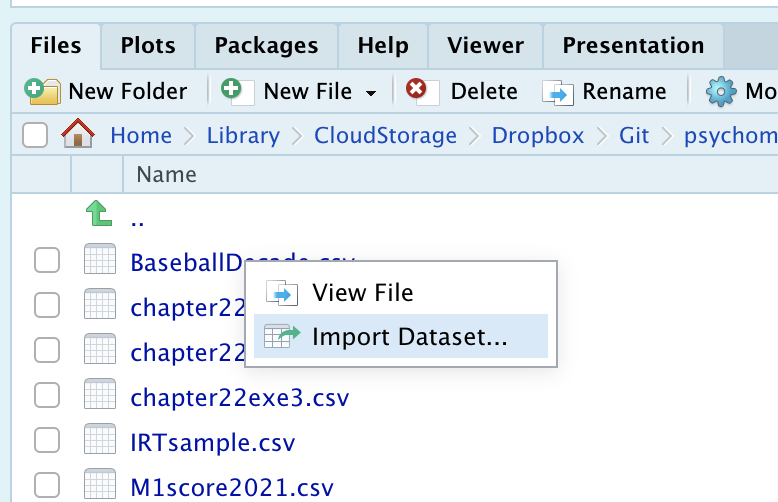
\includegraphics[keepaspectratio]{importDataset.png}}

\subsection{Import Dataset}\label{import-dataset}

\pandocbounded{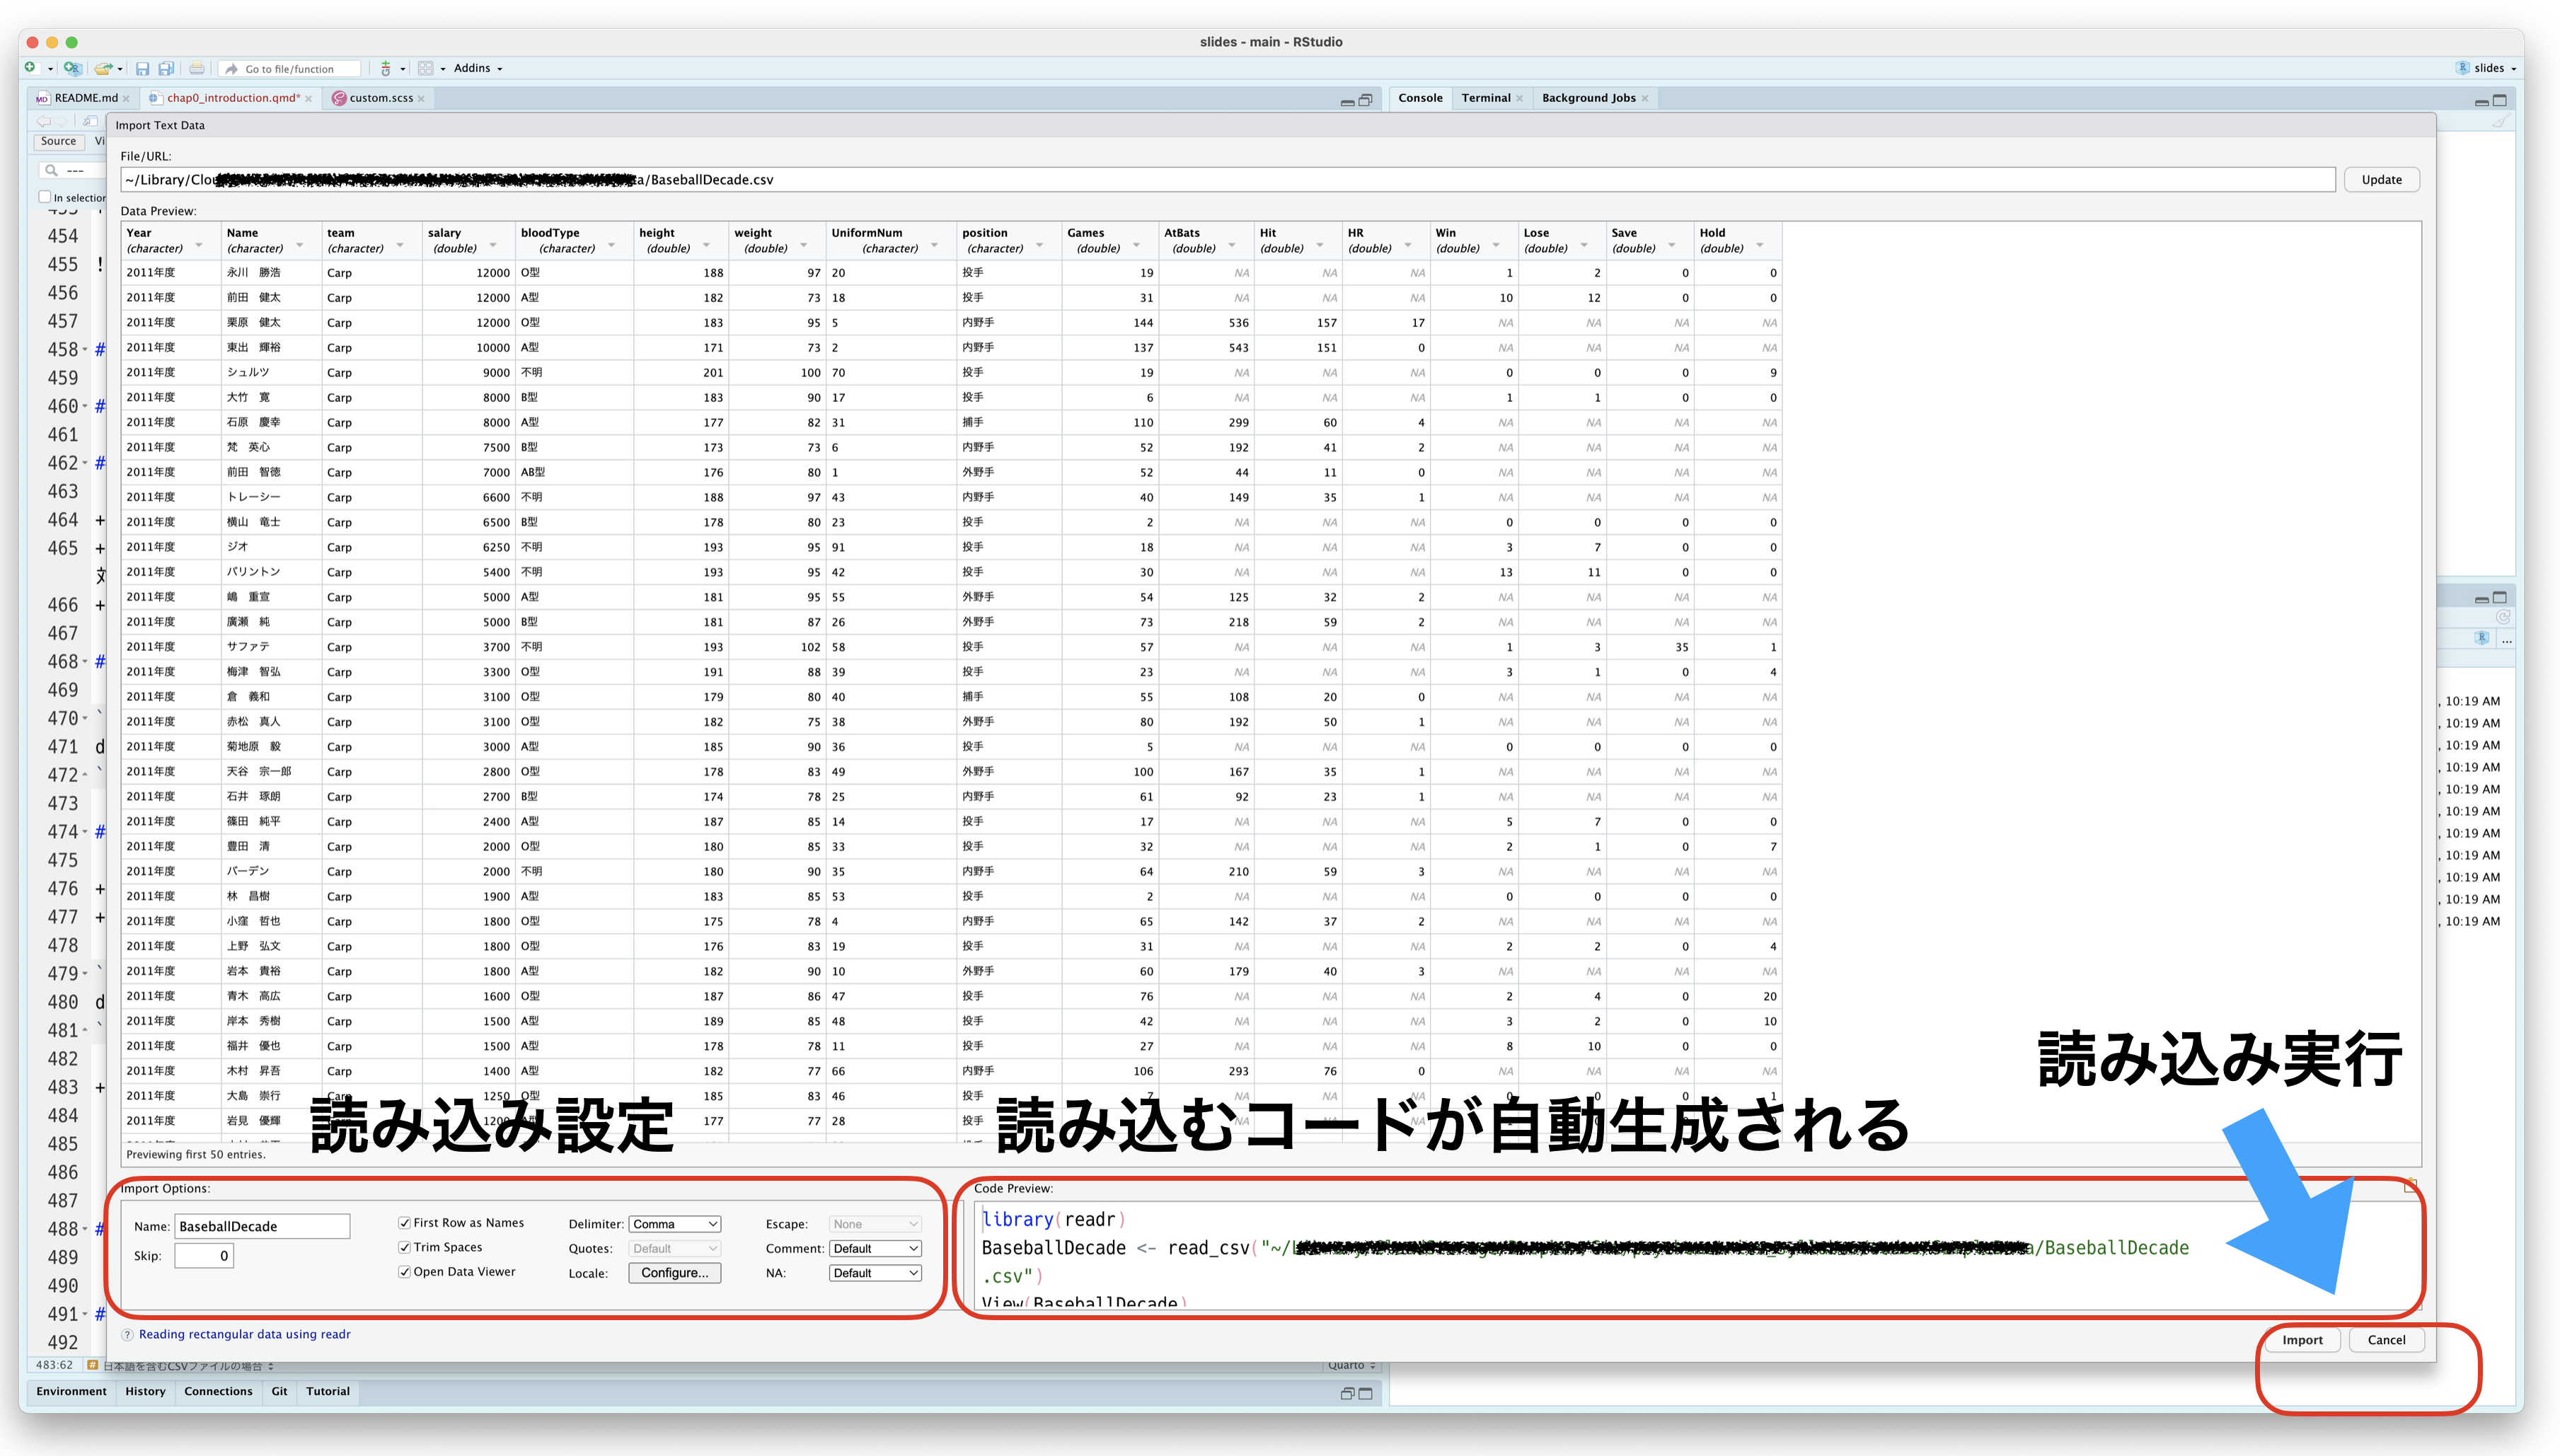
\includegraphics[keepaspectratio]{importDatasetWindow.png}}

\subsection{サンプルコードを読み込んでみよう}\label{ux30b5ux30f3ux30d7ux30ebux30b3ux30fcux30c9ux3092ux8aadux307fux8fbcux3093ux3067ux307fux3088ux3046}

\begin{itemize}
\tightlist
\item
  インターネットから読み込むこともできます!
\item
  次のコードでサンプルデータを読み込んでみましょう。
\end{itemize}

\begin{Shaded}
\begin{Highlighting}[]
\NormalTok{baseball }\OtherTok{\textless{}{-}} \FunctionTok{read.csv}\NormalTok{(}\StringTok{"https://shorturl.at/X4ctc"}\NormalTok{)}
\end{Highlighting}
\end{Shaded}

\begin{itemize}
\tightlist
\item
  ショートURLの参照先は怪しいところではありません。

  \begin{itemize}
  \tightlist
  \item
    https://kosugitti.github.io/psychometrics\_syllabus/codes/SampleData/BaseballDecade.csv
  \item
    私の\href{https://kosugitti.github.io/psychometrics_syllabus/}{心理統計教育教材}サイトに置いてあるサンプルデータです
  \item
    野球選手の基本情報など,10年分のデータがあります。
  \end{itemize}
\item
  データの一部(冒頭)を\texttt{head}関数で確認してみましょう
\end{itemize}

\begin{Shaded}
\begin{Highlighting}[]
\FunctionTok{head}\NormalTok{(baseball)}
\end{Highlighting}
\end{Shaded}

\begin{verbatim}
      Year       Name team salary bloodType height weight UniformNum position
1 2011年度 永川 勝浩 Carp  12000       O型    188     97         20     投手
2 2011年度 前田 健太 Carp  12000       A型    182     73         18     投手
3 2011年度 栗原 健太 Carp  12000       O型    183     95          5   内野手
4 2011年度 東出 輝裕 Carp  10000       A型    171     73          2   内野手
5 2011年度   シュルツ Carp   9000      不明    201    100         70     投手
6 2011年度   大竹 寛 Carp   8000       B型    183     90         17     投手
  Games AtBats Hit HR Win Lose Save Hold
1    19     NA  NA NA   1    2    0    0
2    31     NA  NA NA  10   12    0    0
3   144    536 157 17  NA   NA   NA   NA
4   137    543 151  0  NA   NA   NA   NA
5    19     NA  NA NA   0    0    0    9
6     6     NA  NA NA   1    1    0    0
\end{verbatim}

\subsection{オブジェクトの基本情報}\label{ux30aaux30d6ux30b8ux30a7ux30afux30c8ux306eux57faux672cux60c5ux5831}

\begin{itemize}
\tightlist
\item
  \texttt{str}関数,あるいは\texttt{Environment}タブにあるオブジェクト名を開くと,基本情報が確認できます。
\end{itemize}

\begin{Shaded}
\begin{Highlighting}[]
\FunctionTok{str}\NormalTok{(baseball)}
\end{Highlighting}
\end{Shaded}

\begin{verbatim}
'data.frame':   6546 obs. of  17 variables:
 $ Year      : chr  "2011年度" "2011年度" "2011年度" "2011年度" ...
 $ Name      : chr  "永川 勝浩" "前田 健太" "栗原 健太" "東出 輝裕" ...
 $ team      : chr  "Carp" "Carp" "Carp" "Carp" ...
 $ salary    : int  12000 12000 12000 10000 9000 8000 8000 7500 7000 6600 ...
 $ bloodType : chr  "O型" "A型" "O型" "A型" ...
 $ height    : int  188 182 183 171 201 183 177 173 176 188 ...
 $ weight    : int  97 73 95 73 100 90 82 73 80 97 ...
 $ UniformNum: int  20 18 5 2 70 17 31 6 1 43 ...
 $ position  : chr  "投手" "投手" "内野手" "内野手" ...
 $ Games     : int  19 31 144 137 19 6 110 52 52 40 ...
 $ AtBats    : int  NA NA 536 543 NA NA 299 192 44 149 ...
 $ Hit       : int  NA NA 157 151 NA NA 60 41 11 35 ...
 $ HR        : int  NA NA 17 0 NA NA 4 2 0 1 ...
 $ Win       : int  1 10 NA NA 0 1 NA NA NA NA ...
 $ Lose      : int  2 12 NA NA 0 1 NA NA NA NA ...
 $ Save      : int  0 0 NA NA 0 0 NA NA NA NA ...
 $ Hold      : int  0 0 NA NA 9 0 NA NA NA NA ...
\end{verbatim}

\begin{itemize}
\tightlist
\item
  何年度のデータか(\texttt{Year}),選手名(\texttt{Name}),どのチーム所属か(\texttt{team}),年俸(\texttt{salary})などがあります。
\item
  データの型もわかります

  \begin{itemize}
  \tightlist
  \item
    \texttt{chr}は文字列型です。四則演算の対象ではありません。
  \item
    \texttt{int},\texttt{num}は数字です(整数と実数)
  \item
    \texttt{NA}は欠損値を表しています。
  \end{itemize}
\item
  \texttt{read.csv}関数は読み込んだデータを自動的にデータフレーム型にします。
\end{itemize}

\subsection{記述統計量}\label{ux8a18ux8ff0ux7d71ux8a08ux91cf}

\begin{itemize}
\tightlist
\item
  \texttt{summary}関数で要約統計量を算出できます
\end{itemize}

\begin{Shaded}
\begin{Highlighting}[]
\FunctionTok{summary}\NormalTok{(baseball)}
\end{Highlighting}
\end{Shaded}

\begin{verbatim}
     Year               Name               team               salary     
 Length:6546        Length:6546        Length:6546        Min.   :  200  
 Class :character   Class :character   Class :character   1st Qu.: 1000  
 Mode  :character   Mode  :character   Mode  :character   Median : 2000  
                                                          Mean   : 5178  
                                                          3rd Qu.: 5700  
                                                          Max.   :65000  
                                                                         
  bloodType             height          weight      UniformNum   
 Length:6546        Min.   :163.0   Min.   : 60   Min.   : 0.00  
 Class :character   1st Qu.:177.0   1st Qu.: 78   1st Qu.:16.00  
 Mode  :character   Median :180.0   Median : 83   Median :33.00  
                    Mean   :180.7   Mean   : 84   Mean   :34.93  
                    3rd Qu.:184.0   3rd Qu.: 89   3rd Qu.:52.00  
                    Max.   :216.0   Max.   :135   Max.   :99.00  
                                                                 
   position             Games            AtBats           Hit        
 Length:6546        Min.   :  1.00   Min.   :  0.0   Min.   :  0.00  
 Class :character   1st Qu.:  9.00   1st Qu.: 23.0   1st Qu.:  4.00  
 Mode  :character   Median : 25.00   Median : 95.0   Median : 21.00  
                    Mean   : 40.67   Mean   :165.1   Mean   : 42.53  
                    3rd Qu.: 61.00   3rd Qu.:271.0   3rd Qu.: 69.00  
                    Max.   :144.00   Max.   :603.0   Max.   :216.00  
                                     NA's   :3233    NA's   :3233    
       HR              Win              Lose             Save      
 Min.   : 0.000   Min.   : 0.000   Min.   : 0.000   Min.   : 0.00  
 1st Qu.: 0.000   1st Qu.: 0.000   1st Qu.: 0.000   1st Qu.: 0.00  
 Median : 1.000   Median : 1.000   Median : 1.000   Median : 0.00  
 Mean   : 3.967   Mean   : 2.517   Mean   : 2.509   Mean   : 1.27  
 3rd Qu.: 4.000   3rd Qu.: 4.000   3rd Qu.: 4.000   3rd Qu.: 0.00  
 Max.   :60.000   Max.   :24.000   Max.   :15.000   Max.   :54.00  
 NA's   :3233     NA's   :3307     NA's   :3307     NA's   :3307   
      Hold       
 Min.   : 0.000  
 1st Qu.: 0.000  
 Median : 0.000  
 Mean   : 3.511  
 3rd Qu.: 3.000  
 Max.   :45.000  
 NA's   :3307    
\end{verbatim}

\begin{itemize}
\tightlist
\item
  行数,列数を確認して,データのサイズを見ておきましょう
\end{itemize}

\begin{Shaded}
\begin{Highlighting}[]
\FunctionTok{NROW}\NormalTok{(baseball)}
\end{Highlighting}
\end{Shaded}

\begin{verbatim}
[1] 6546
\end{verbatim}

\begin{Shaded}
\begin{Highlighting}[]
\FunctionTok{NCOL}\NormalTok{(baseball)}
\end{Highlighting}
\end{Shaded}

\begin{verbatim}
[1] 17
\end{verbatim}

\subsection{変数毎の要約統計量}\label{ux5909ux6570ux6bceux306eux8981ux7d04ux7d71ux8a08ux91cf}

\begin{itemize}
\tightlist
\item
  変数に\texttt{\$}でアクセスして,要約統計量を計算してみましょう。
\end{itemize}

\begin{Shaded}
\begin{Highlighting}[]
\FunctionTok{mean}\NormalTok{(baseball}\SpecialCharTok{$}\NormalTok{height)}
\end{Highlighting}
\end{Shaded}

\begin{verbatim}
[1] 180.7177
\end{verbatim}

\begin{Shaded}
\begin{Highlighting}[]
\FunctionTok{sd}\NormalTok{(baseball}\SpecialCharTok{$}\NormalTok{height)}
\end{Highlighting}
\end{Shaded}

\begin{verbatim}
[1] 5.613504
\end{verbatim}

\begin{Shaded}
\begin{Highlighting}[]
\FunctionTok{median}\NormalTok{(baseball}\SpecialCharTok{$}\NormalTok{weight)}
\end{Highlighting}
\end{Shaded}

\begin{verbatim}
[1] 83
\end{verbatim}

\begin{Shaded}
\begin{Highlighting}[]
\FunctionTok{max}\NormalTok{(baseball}\SpecialCharTok{$}\NormalTok{salary)}
\end{Highlighting}
\end{Shaded}

\begin{verbatim}
[1] 65000
\end{verbatim}

\begin{Shaded}
\begin{Highlighting}[]
\FunctionTok{min}\NormalTok{(baseball}\SpecialCharTok{$}\NormalTok{salary)}
\end{Highlighting}
\end{Shaded}

\begin{verbatim}
[1] 200
\end{verbatim}

\begin{Shaded}
\begin{Highlighting}[]
\FunctionTok{quantile}\NormalTok{(baseball}\SpecialCharTok{$}\NormalTok{salary)}
\end{Highlighting}
\end{Shaded}

\begin{verbatim}
   0%   25%   50%   75%  100% 
  200  1000  2000  5700 65000 
\end{verbatim}

\subsection{因子型をつくってみましょう}\label{ux56e0ux5b50ux578bux3092ux3064ux304fux3063ux3066ux307fux307eux3057ux3087ux3046}

\begin{itemize}
\tightlist
\item
  チーム名はたかだか12種類です。名義尺度水準+ラベルの数値であるFactor型にしてみましょう。
\end{itemize}

\begin{Shaded}
\begin{Highlighting}[]
\NormalTok{baseball}\SpecialCharTok{$}\NormalTok{team }\OtherTok{\textless{}{-}} \FunctionTok{as.factor}\NormalTok{(baseball}\SpecialCharTok{$}\NormalTok{team)}
\FunctionTok{summary}\NormalTok{(baseball}\SpecialCharTok{$}\NormalTok{team)}
\end{Highlighting}
\end{Shaded}

\begin{verbatim}
    Carp     DeNA  Dragons   Eagles Fighters   Giants    Lions    Lotte 
     517      550      573      569      533      524      528      538 
    Orix Softbank Swallows   Tigers 
     579      525      556      554 
\end{verbatim}

\begin{itemize}
\tightlist
\item
  一行目で,同じ変数に「上書き」していることに注意
\item
  \texttt{as.factor}関数は変数をFactor型に変換するものです

  \begin{itemize}
  \tightlist
  \item
    クラス名,実験の水準などグループ化変数として扱うのに便利です
  \end{itemize}
\end{itemize}

\subsection{可視化してみましょう}\label{ux53efux8996ux5316ux3057ux3066ux307fux307eux3057ux3087ux3046}

\begin{itemize}
\tightlist
\item
  \textbf{データは図にする}のが基本です。Rの基本関数でも十分綺麗な図が描けます。

  \begin{itemize}
  \tightlist
  \item
    ヒットの数をヒストグラムにしてみましょう
  \item
    ヒストグラムの関数は\texttt{hist}です
  \end{itemize}
\end{itemize}

\begin{Shaded}
\begin{Highlighting}[]
\FunctionTok{print}\NormalTok{(}\FunctionTok{head}\NormalTok{(baseball))}
\end{Highlighting}
\end{Shaded}

\begin{verbatim}
      Year       Name team salary bloodType height weight UniformNum position
1 2011年度 永川 勝浩 Carp  12000       O型    188     97         20     投手
2 2011年度 前田 健太 Carp  12000       A型    182     73         18     投手
3 2011年度 栗原 健太 Carp  12000       O型    183     95          5   内野手
4 2011年度 東出 輝裕 Carp  10000       A型    171     73          2   内野手
5 2011年度   シュルツ Carp   9000      不明    201    100         70     投手
6 2011年度   大竹 寛 Carp   8000       B型    183     90         17     投手
  Games AtBats Hit HR Win Lose Save Hold
1    19     NA  NA NA   1    2    0    0
2    31     NA  NA NA  10   12    0    0
3   144    536 157 17  NA   NA   NA   NA
4   137    543 151  0  NA   NA   NA   NA
5    19     NA  NA NA   0    0    0    9
6     6     NA  NA NA   1    1    0    0
\end{verbatim}

\begin{Shaded}
\begin{Highlighting}[]
\FunctionTok{print}\NormalTok{(}\FunctionTok{class}\NormalTok{(baseball}\SpecialCharTok{$}\NormalTok{Hit))}
\end{Highlighting}
\end{Shaded}

\begin{verbatim}
[1] "integer"
\end{verbatim}

\begin{Shaded}
\begin{Highlighting}[]
\FunctionTok{hist}\NormalTok{(baseball}\SpecialCharTok{$}\NormalTok{Hit)}
\end{Highlighting}
\end{Shaded}

\pandocbounded{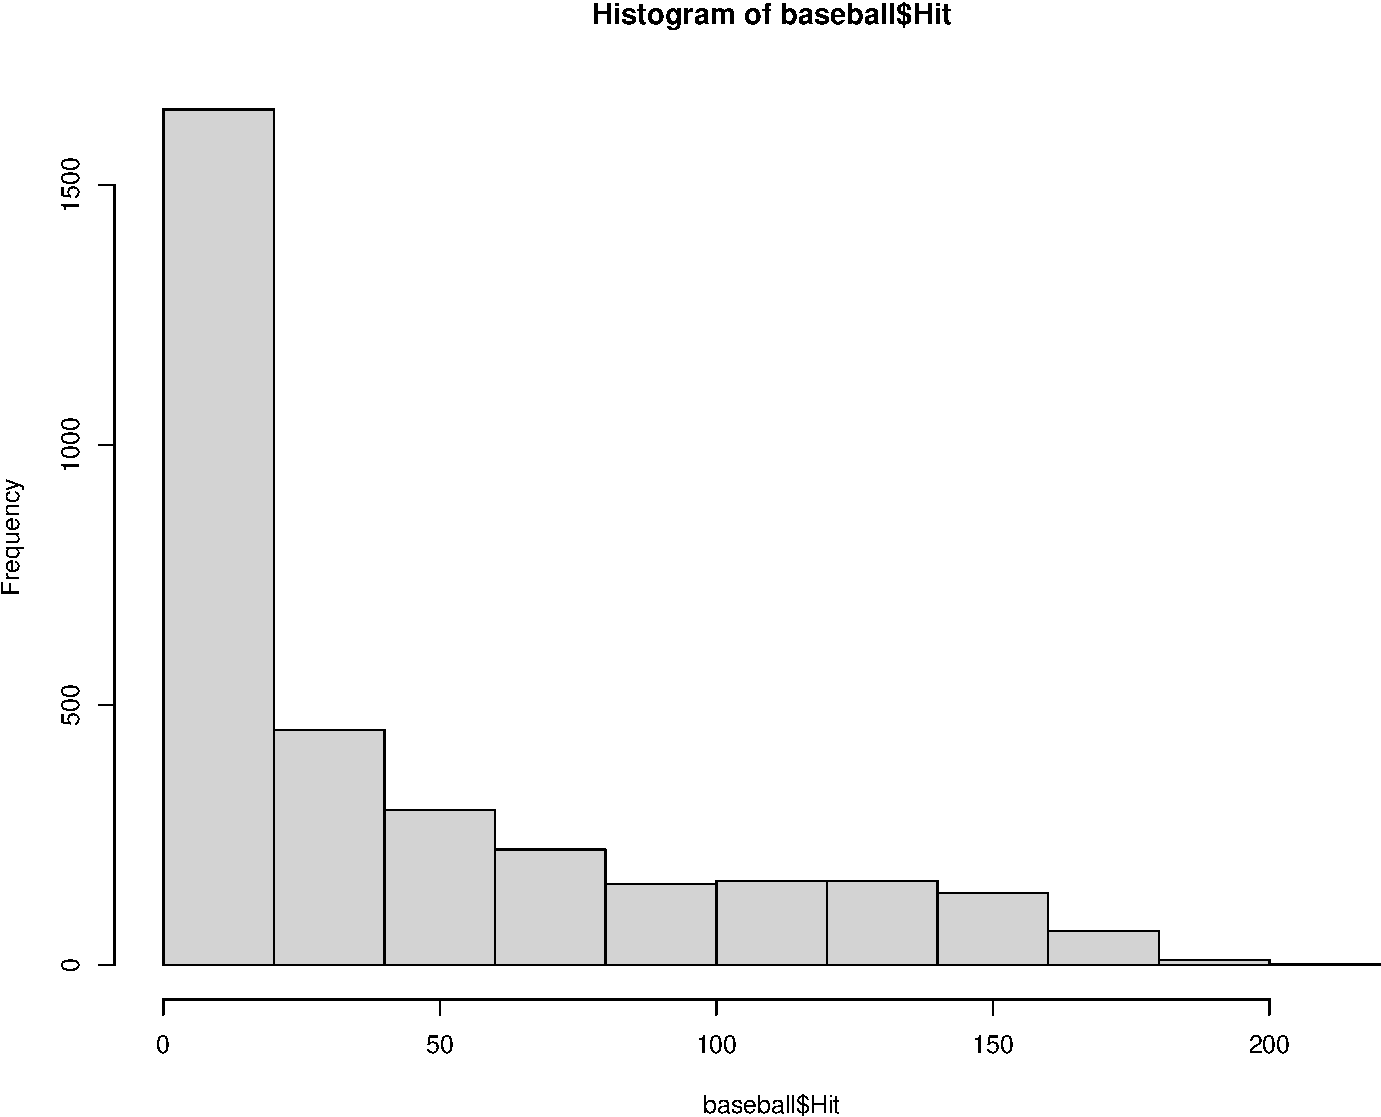
\includegraphics[keepaspectratio]{chap0_introduction_files/figure-pdf/plot1-1.pdf}}

\subsection{可視化してみましょう}\label{ux53efux8996ux5316ux3057ux3066ux307fux307eux3057ux3087ux3046-1}

\begin{itemize}
\tightlist
\item
  \textbf{データは図にする}のが基本です。

  \begin{itemize}
  \tightlist
  \item
    チーム毎のヒット数の違いを見てみましょう
  \item
    ボックスプロット(箱ひげ図)の関数は\texttt{boxplot}です

    \begin{itemize}
    \tightlist
    \item
      x軸がFactor型になっています
    \end{itemize}
  \end{itemize}
\end{itemize}

\begin{Shaded}
\begin{Highlighting}[]
\FunctionTok{boxplot}\NormalTok{(Hit }\SpecialCharTok{\textasciitilde{}}\NormalTok{ team, }\AttributeTok{data =}\NormalTok{ baseball)}
\end{Highlighting}
\end{Shaded}

\pandocbounded{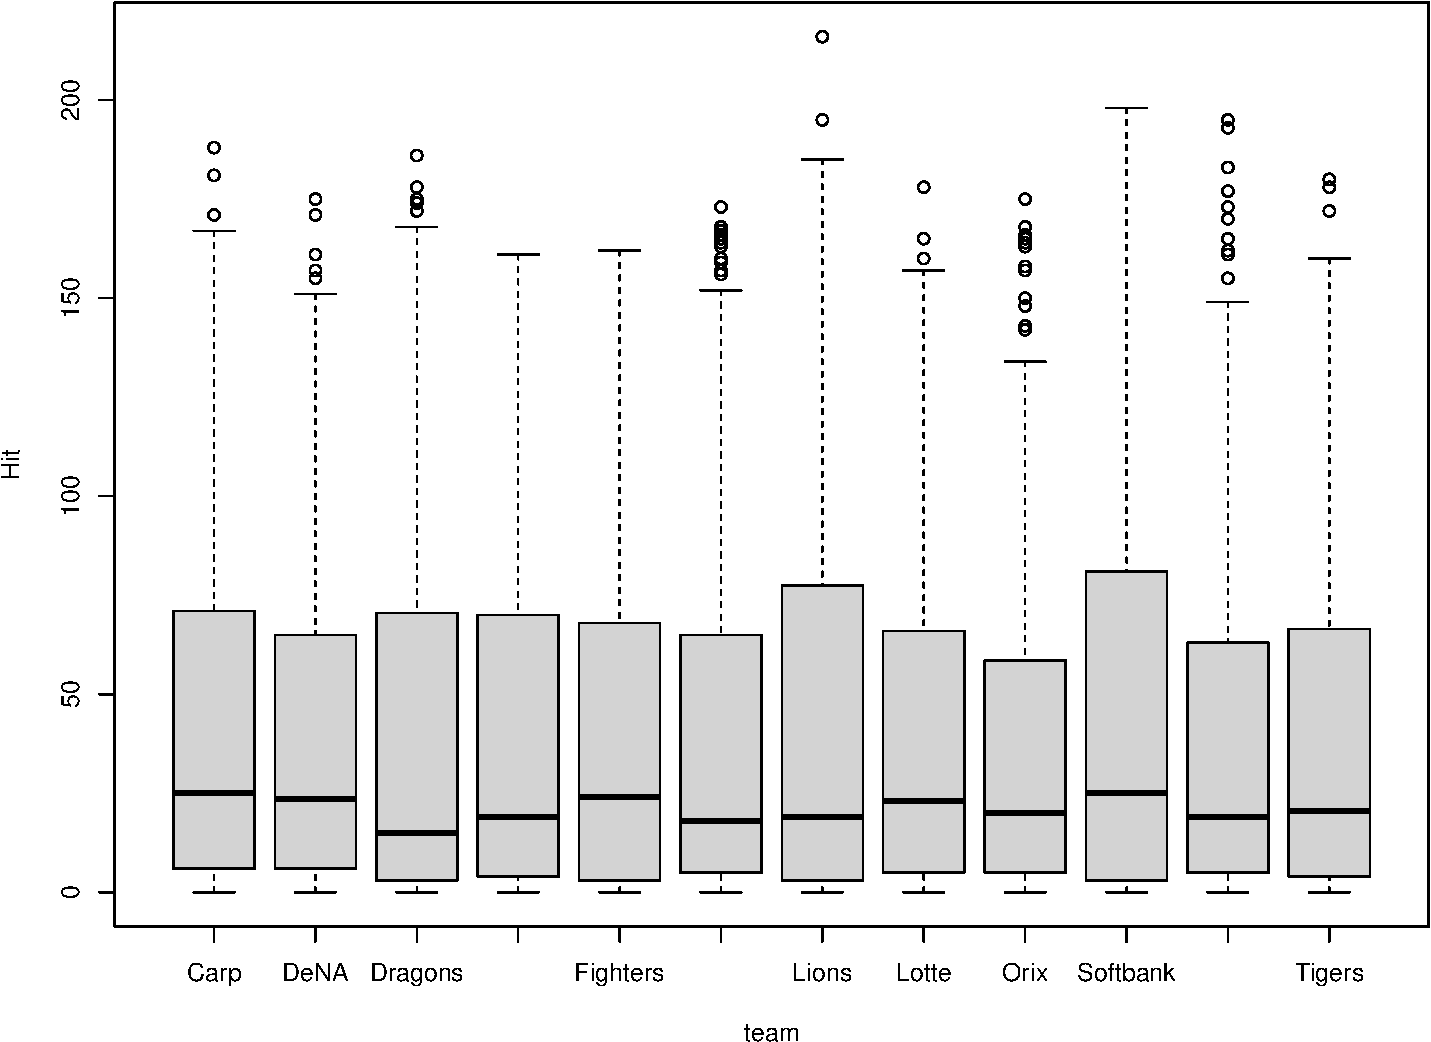
\includegraphics[keepaspectratio]{chap0_introduction_files/figure-pdf/plot2-1.pdf}}

\subsection{可視化してみましょう}\label{ux53efux8996ux5316ux3057ux3066ux307fux307eux3057ux3087ux3046-2}

\begin{itemize}
\tightlist
\item
  \textbf{データは図にする}のが基本です。

  \begin{itemize}
  \tightlist
  \item
    散布図を書いてみましょう
  \item
    散布図は\texttt{plot}関数にx軸とy軸変数を指定します
  \end{itemize}
\end{itemize}

\begin{Shaded}
\begin{Highlighting}[]
\FunctionTok{plot}\NormalTok{(baseball}\SpecialCharTok{$}\NormalTok{height, baseball}\SpecialCharTok{$}\NormalTok{weight)}
\end{Highlighting}
\end{Shaded}

\pandocbounded{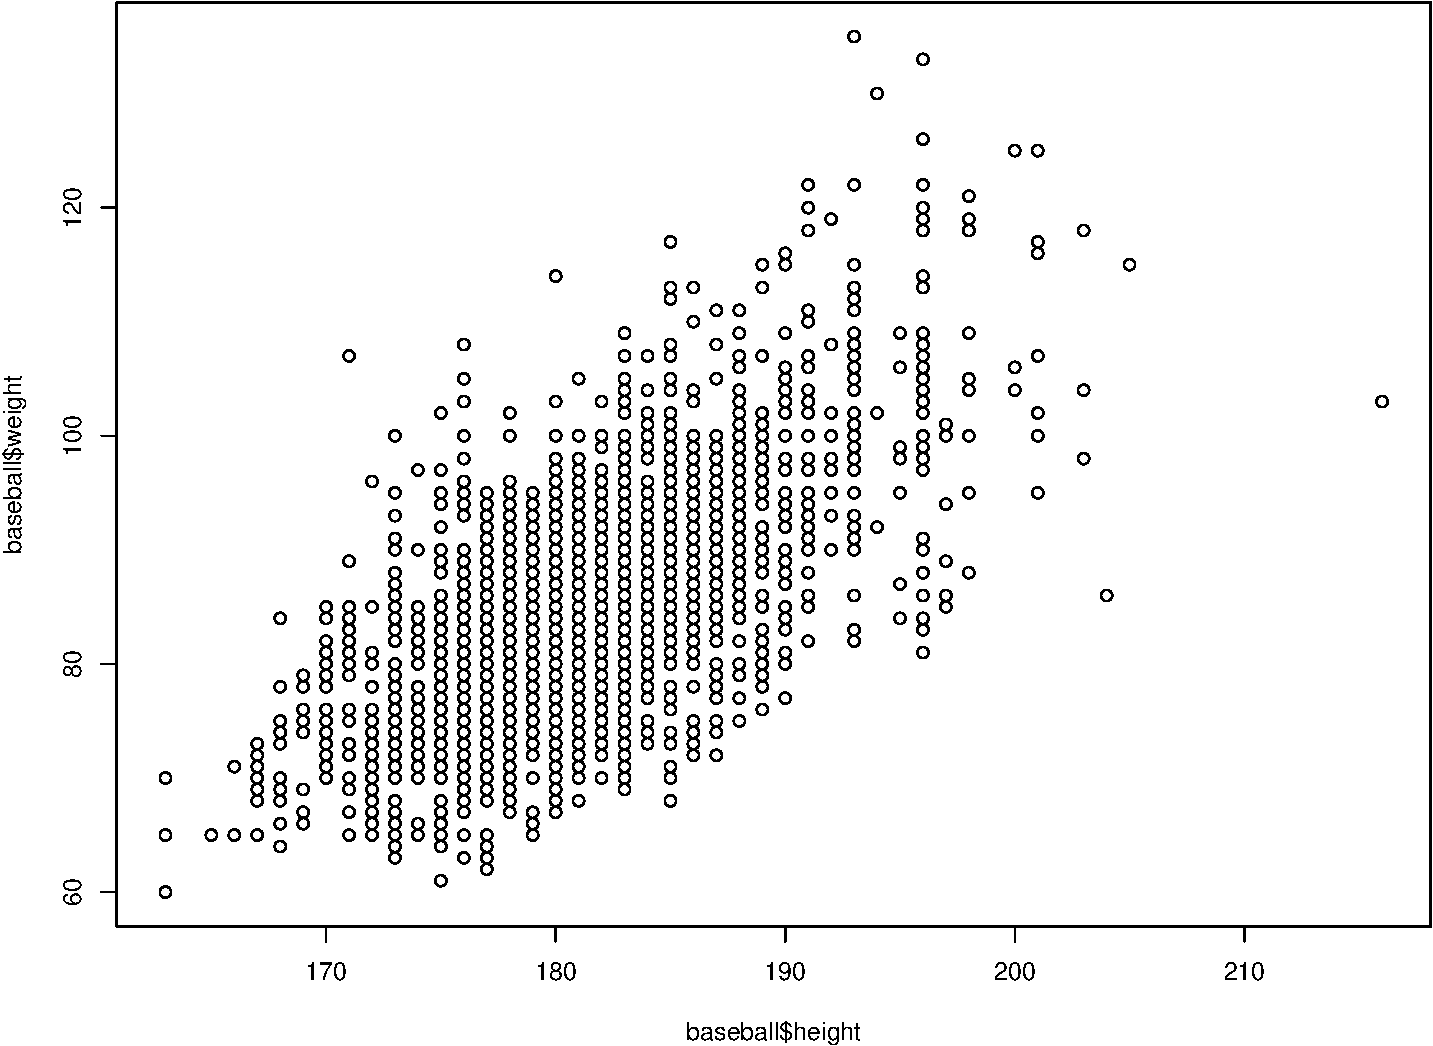
\includegraphics[keepaspectratio]{chap0_introduction_files/figure-pdf/plot3-1.pdf}}

\subsection{(余談)ggplotによる出力は,より綺麗です}\label{ux4f59ux8ac7ggplotux306bux3088ux308bux51faux529bux306fux3088ux308aux7dbaux9e97ux3067ux3059}

\begin{Shaded}
\begin{Highlighting}[]
\FunctionTok{library}\NormalTok{(ggplot2)}
\NormalTok{baseball }\SpecialCharTok{|\textgreater{}}
    \FunctionTok{ggplot}\NormalTok{(}\FunctionTok{aes}\NormalTok{(}\AttributeTok{x =}\NormalTok{ weight, }\AttributeTok{y =}\NormalTok{ height, }\AttributeTok{color =}\NormalTok{ team)) }\SpecialCharTok{+}
    \FunctionTok{geom\_point}\NormalTok{() }\SpecialCharTok{+}
    \FunctionTok{geom\_smooth}\NormalTok{(}\AttributeTok{formula =} \StringTok{"y \textasciitilde{} x"}\NormalTok{, }\AttributeTok{method =} \StringTok{"lm"}\NormalTok{, }\AttributeTok{se =} \ConstantTok{FALSE}\NormalTok{) }\SpecialCharTok{+}
    \FunctionTok{facet\_wrap}\NormalTok{(}\SpecialCharTok{\textasciitilde{}}\NormalTok{team)}
\end{Highlighting}
\end{Shaded}

\pandocbounded{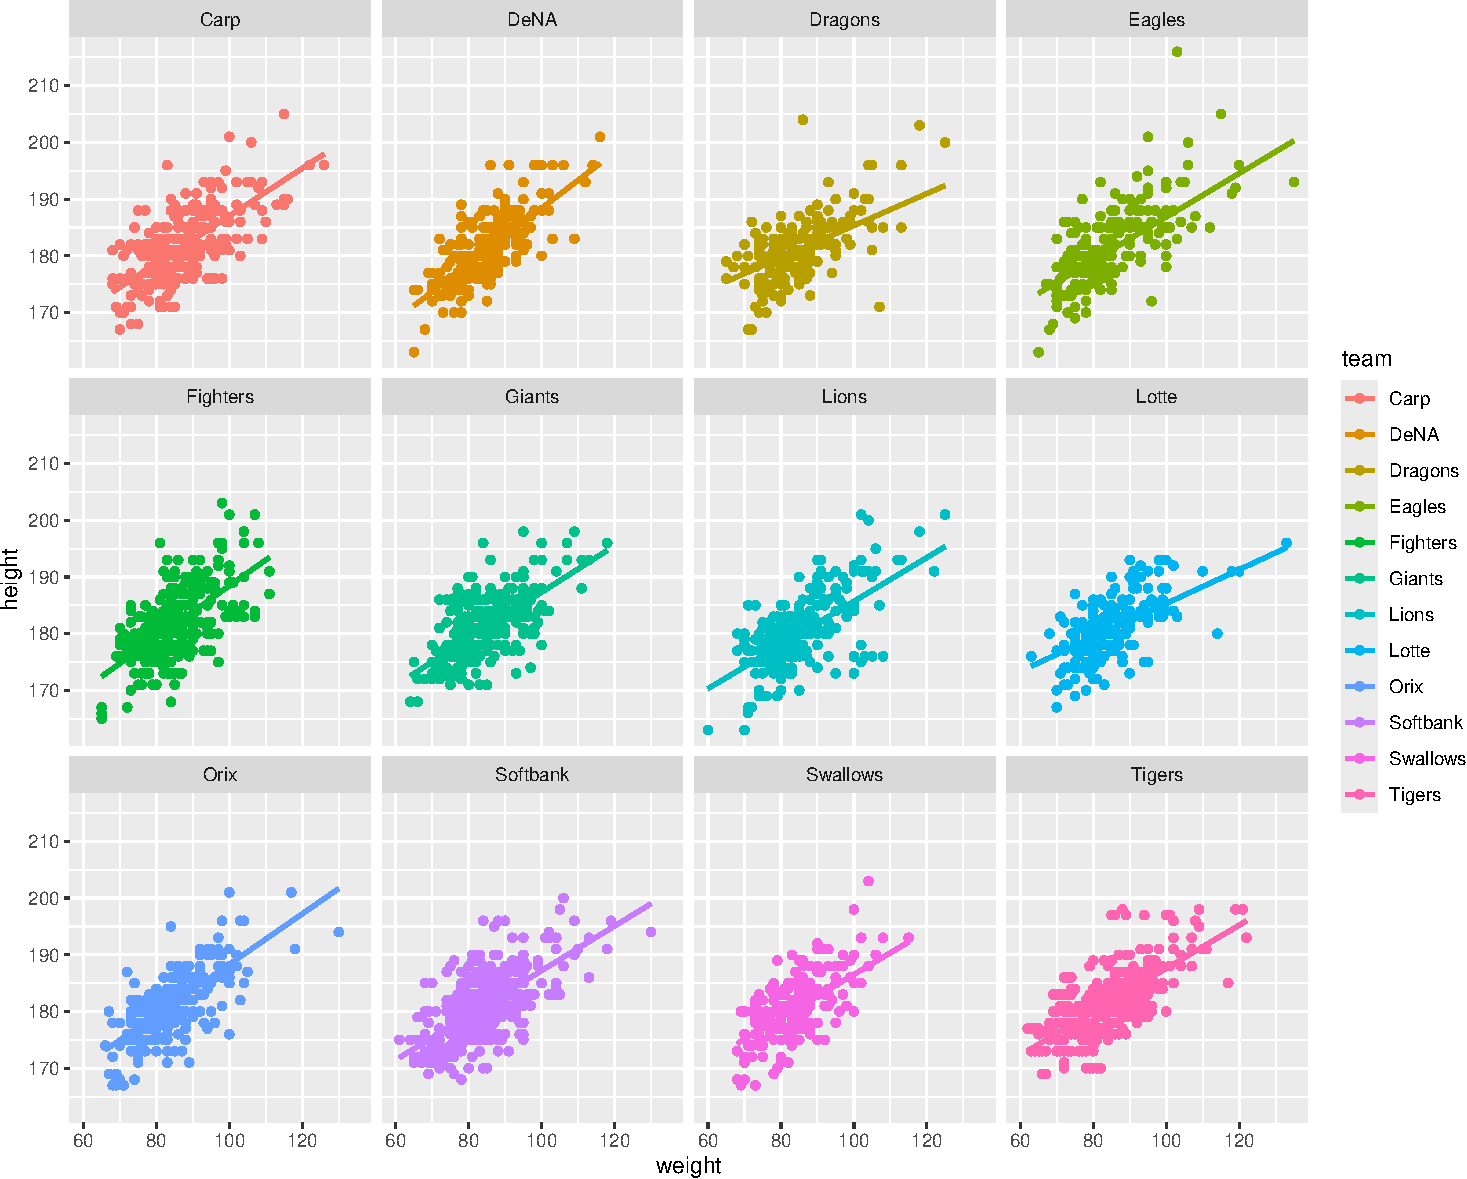
\includegraphics[keepaspectratio]{chap0_introduction_files/figure-pdf/ggplot1-1.pdf}}

\section{Enjoy!}\label{enjoy}

\begin{itemize}
\tightlist
\item
  以上で入門コースは終了です
\item
  この講義では\texttt{exametrika}パッケージの他は,基本的にRの基本関数だけで分析できるようにご案内します。
\item
  実は\texttt{ggexametrika}パッケージというのもあります→\href{https://github.com/kosugitti/ggExametrika}{こちら}
\end{itemize}

\section{あなうんすめんと}\label{ux3042ux306aux3046ux3093ux3059ux3081ux3093ux3068}

\subsection{\texorpdfstring{\texttt{exametrika} Web
site}{exametrika Web site}}\label{exametrika-web-site}

\begin{itemize}
\tightlist
\item
  \href{https://kosugitti.github.io/exametrika/}{exametrikaのサイトはこちら}
\end{itemize}

\subsubsection{問題の報告}\label{ux554fux984cux306eux5831ux544a}

バグを発見した場合や改善の提案がある場合:

\begin{itemize}
\tightlist
\item
  \href{https://github.com/kosugitti/exametrika/issues}{GitHub
  Issues}にIssueを開いてください
\item
  最小限の再現可能な例を提供してください
\item
  Rのセッション情報(sessionInfo())を含めてください
\end{itemize}

\subsubsection{ディスカッションとコミュニティ}\label{ux30c7ux30a3ux30b9ux30abux30c3ux30b7ux30e7ux30f3ux3068ux30b3ux30dfux30e5ux30cbux30c6ux30a3}

\begin{itemize}
\item
  \href{https://github.com/kosugitti/exametrika/discussions}{Github
  Discussions}では,次のことができます。
\item
  質問をする
\item
  使用事例を共有する
\item
  機能リクエストについて議論する
\item
  ヒントやコツを交換する
\item
  パッケージの開発に関する最新情報を得る
\end{itemize}

\section{Advanced Topics}\label{advanced-topics}

\subsection{Quarto/Rmarkdown:文芸的プログラミング}\label{quartormarkdownux6587ux82b8ux7684ux30d7ux30edux30b0ux30e9ux30dfux30f3ux30b0}

\subsubsection{Rmarkdownとは}\label{rmarkdownux3068ux306f}

\begin{itemize}
\item
  Markdown書式というプレーンな文書作成文法 +
  チャンクと呼ばれるRコードの結合
\item
  文書を作成(レンダリング)するときは,Rの計算を実行してその結果を文書内に反映させる
\item
  コピペ汚染がなく,RStudioで執筆と分析が統合,これだけで完結できます。
\end{itemize}

\subsubsection{Quartoとは}\label{quartoux3068ux306f}

\begin{itemize}
\tightlist
\item
  次世代のR Markdownです。私のスライドもQuartoで作られています
\item
  マルチ言語対応(R, Python, Julia等)
\item
  ePub, PDFなど出力も多様
\end{itemize}

\subsection{Quarto/Rmarkdown:文芸的プログラミング}\label{quartormarkdownux6587ux82b8ux7684ux30d7ux30edux30b0ux30e9ux30dfux30f3ux30b0-1}

\subsubsection{基本的な使い方}\label{ux57faux672cux7684ux306aux4f7fux3044ux65b9-1}

\begin{enumerate}
\def\labelenumi{\arabic{enumi}.}
\tightlist
\item
  File → New FileでQuarto Document / R Markdownを選択
\item
  TitleやAuthorを入力,出力書式(HTML,PDF,Word)などを選ぶ画面が出ます
\item
  サンプル文書・コードが書いてあるファイルが生成されます
\end{enumerate}

これをRneder/Knitすることでファイルが出力されます。

\bookmarksetup{startatroot}

\chapter{Rをつかった項目分析の実習}\label{rux3092ux3064ux304bux3063ux305fux9805ux76eeux5206ux6790ux306eux5b9fux7fd2}

\section{準備しましょう}\label{ux6e96ux5099ux3057ux307eux3057ux3087ux3046}

\begin{itemize}
\tightlist
\item
  項目分析を実行するにあたって準備するもの

  \begin{itemize}
  \tightlist
  \item
    \texttt{exametrika}パッケージ
  \item
    データ
  \end{itemize}
\item
  データはテストデータを基本とします

  \begin{itemize}
  \tightlist
  \item
    テストデータは正答を\texttt{1},
    誤答を\texttt{0}とコーディングしたもの
  \item
    欠損値はRの\texttt{NA}か,\texttt{-999}のようにありえない数値にしているもの
  \end{itemize}
\item
  \texttt{exametrika}では

  \begin{itemize}
  \tightlist
  \item
    データは行列でもデータフレームでもOK
  \item
    パッケージの中では,一旦どういうデータ形式かを判断して,そのデータ形式に合わせて処理を行います
  \end{itemize}
\end{itemize}

\section{CSVファイルから読み込む場合(1/2)}\label{csvux30d5ux30a1ux30a4ux30ebux304bux3089ux8aadux307fux8fbcux3080ux5834ux540812}

\begin{itemize}
\tightlist
\item
  データをCSVファイルで保存したとします
\end{itemize}

\begin{figure}[H]

{\centering \pandocbounded{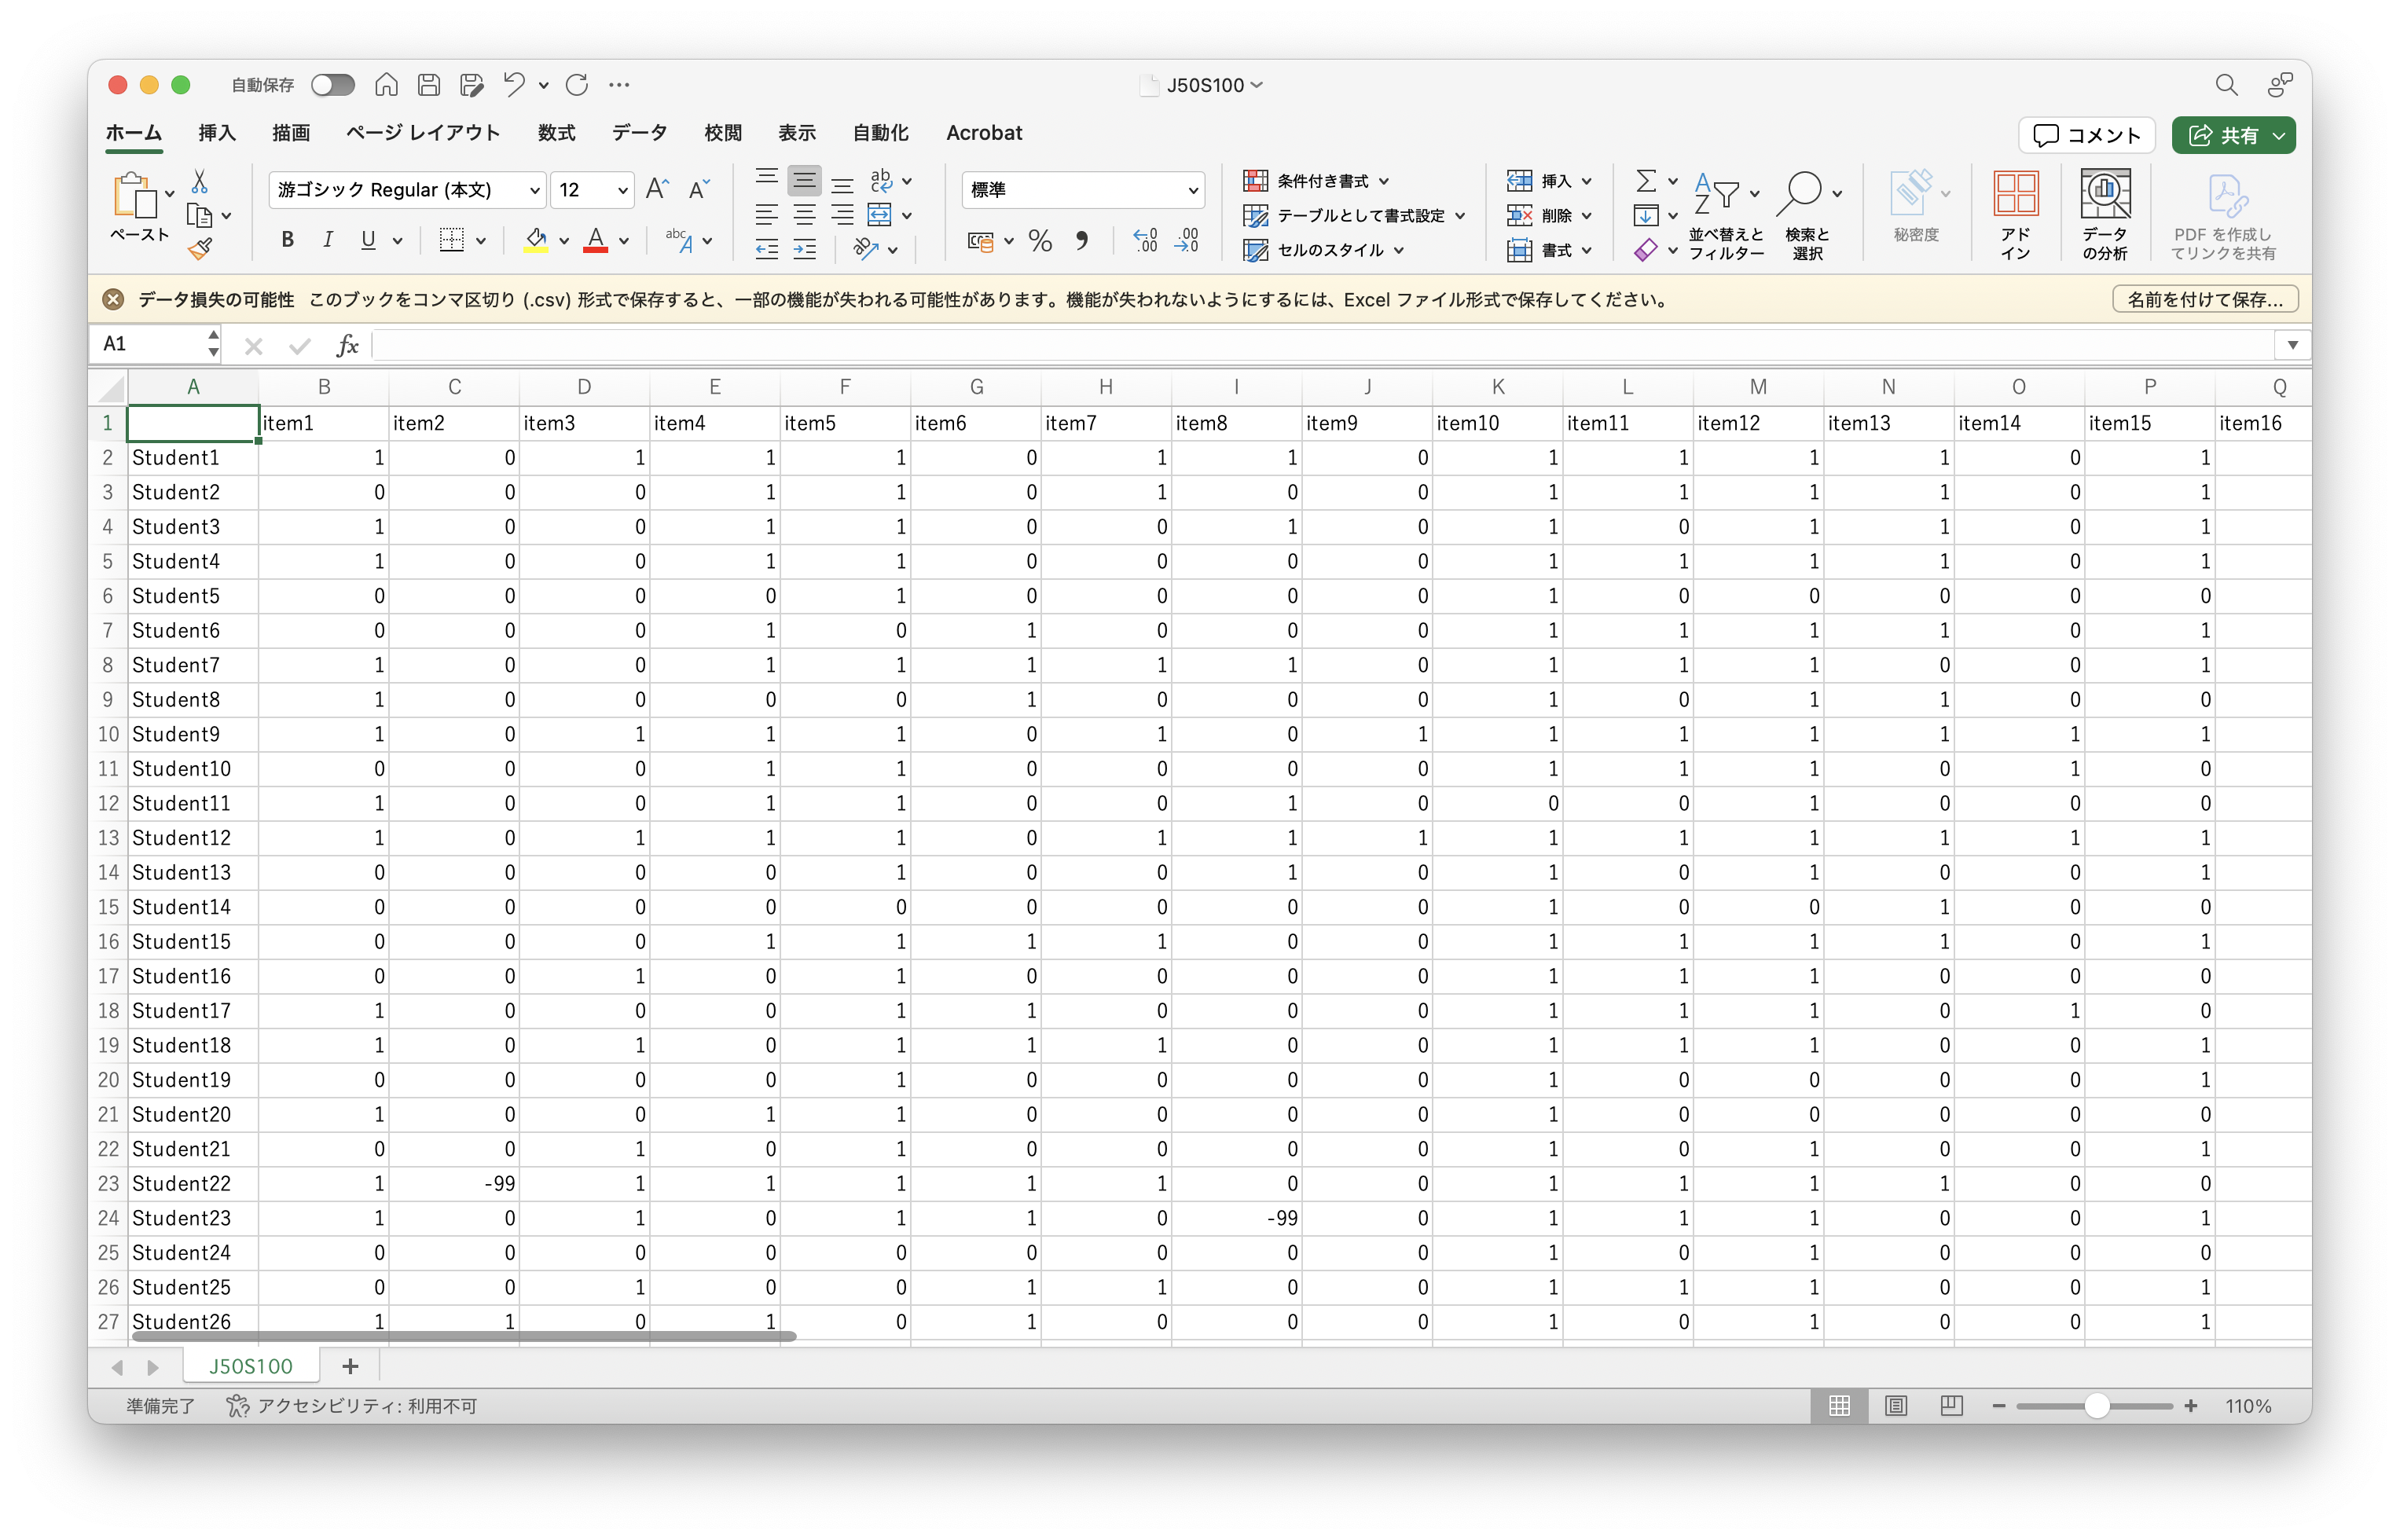
\includegraphics[keepaspectratio]{sampleJ50S100.png}}

}

\caption{csvデータの例}

\end{figure}%

\section{CSVファイルから読み込む場合(2/2)}\label{csvux30d5ux30a1ux30a4ux30ebux304bux3089ux8aadux307fux8fbcux3080ux5834ux540822}

\begin{itemize}
\tightlist
\item
  プロジェクトフォルダに\texttt{J50S100.csv}を保存してください
\item
  このデータを読み込むには,\texttt{read.csv}関数を使います
\end{itemize}

\begin{Shaded}
\begin{Highlighting}[]
\NormalTok{rawData }\OtherTok{\textless{}{-}} \FunctionTok{read.csv}\NormalTok{(}\StringTok{"J50S100.csv"}\NormalTok{)}
\FunctionTok{head}\NormalTok{(rawData)}
\end{Highlighting}
\end{Shaded}

\begin{verbatim}
         X item1 item2 item3 item4 item5 item6 item7 item8 item9 item10 item11
1 Student1     1     0     1     1     1     0     1     1     0      1      1
2 Student2     0     0     0     1     1     0     1     0     0      1      1
3 Student3     1     0     0     1     1     0     0     1     0      1      0
4 Student4     1     0     0     1     1     0     0     0     0      1      1
5 Student5     0     0     0     0     1     0     0     0     0      1      0
6 Student6     0     0     0     1     0     1     0     0     0      1      1
  item12 item13 item14 item15 item16 item17 item18 item19 item20 item21 item22
1      1      1      0      1      1      0      0      1    -99      0      1
2      1      1      0      1      1      0      0      0      1      1      1
3      1      1      0      1      1      0      0      0      1      1      1
4      1      1      0      1      1      0      0      1      1      0      1
5      0      0      0      0      1      0      0      0      1      1      1
6      1      1      0      1      1      0      0      1      1      0    -99
  item23 item24 item25 item26 item27 item28 item29 item30 item31 item32 item33
1      1      0      0      0      0      0      1      1      1      0      1
2      0      0      0      0      1      1      1    -99      0      0      1
3      0      0      0      0      1      0      0      0      1      0      0
4      1      0      0      1      0      1      1      0      0      0      0
5      1    -99      0      0      1      1      0      0      0      0      0
6      1      0      0      0      0      1      1      0      0      0      0
  item34 item35 item36 item37 item38 item39 item40 item41 item42 item43 item44
1      0      1      0      1      0      0      1      1      0      0      1
2      0      0      0      0      0      0      0      1      0      0      1
3      0      0      0      0      1      1      0      0      1      0      1
4      0      1      0      0    -99      0      1      0      0      0      0
5      0      1      0      0      1      0      0      1      1      0      1
6      0      0      0      1      1      1      0      1      0      0      0
  item45 item46 item47 item48 item49 item50
1      1      0      1      0      1      1
2      1      0      0      0      1      0
3      1      1      1      0      0      0
4      1      0      1      0      1      1
5      1      0      0      0      1      1
6      1      1      1      0      0      0
\end{verbatim}

\section{exametrikaの中ではデータが変換されます}\label{exametrikaux306eux4e2dux3067ux306fux30c7ux30fcux30bfux304cux5909ux63dbux3055ux308cux307eux3059}

\begin{itemize}
\tightlist
\item
  \texttt{exametrika}では,データを読み込んだ後,\texttt{dataFormat}関数を使って型変換を行います。
\item
  この関数は各モデルで最初に実行されるので,基本的にユーザが明示的に行う必要はありません。

  \begin{itemize}
  \tightlist
  \item
    多値データで指定が必要なこともあります
  \end{itemize}
\end{itemize}

\begin{Shaded}
\begin{Highlighting}[]
\FunctionTok{library}\NormalTok{(exametrika)}
\end{Highlighting}
\end{Shaded}

\begin{verbatim}
Loading required package: mvtnorm
\end{verbatim}

\begin{verbatim}
Loading required package: igraph
\end{verbatim}

\begin{verbatim}

Attaching package: 'igraph'
\end{verbatim}

\begin{verbatim}
The following objects are masked from 'package:stats':

    decompose, spectrum
\end{verbatim}

\begin{verbatim}
The following object is masked from 'package:base':

    union
\end{verbatim}

\begin{Shaded}
\begin{Highlighting}[]
\NormalTok{dat }\OtherTok{\textless{}{-}} \FunctionTok{dataFormat}\NormalTok{(rawData, }\AttributeTok{na =} \SpecialCharTok{{-}}\DecValTok{99}\NormalTok{)}
\end{Highlighting}
\end{Shaded}

\section{exametrikaクラスのデータ}\label{exametrikaux30afux30e9ux30b9ux306eux30c7ux30fcux30bf}

\begin{itemize}
\tightlist
\item
  データ行列は\(U\),欠測指示子行列は\(Z\)として変換されます。
\end{itemize}

\begin{Shaded}
\begin{Highlighting}[]
\FunctionTok{head}\NormalTok{(dat}\SpecialCharTok{$}\NormalTok{U)}
\end{Highlighting}
\end{Shaded}

\begin{verbatim}
     item1 item2 item3 item4 item5 item6 item7 item8 item9 item10 item11 item12
[1,]     1     0     1     1     1     0     1     1     0      1      1      1
[2,]     0     0     0     1     1     0     1     0     0      1      1      1
[3,]     1     0     0     1     1     0     0     1     0      1      0      1
[4,]     1     0     0     1     1     0     0     0     0      1      1      1
[5,]     0     0     0     0     1     0     0     0     0      1      0      0
[6,]     0     0     0     1     0     1     0     0     0      1      1      1
     item13 item14 item15 item16 item17 item18 item19 item20 item21 item22
[1,]      1      0      1      1      0      0      1     -1      0      1
[2,]      1      0      1      1      0      0      0      1      1      1
[3,]      1      0      1      1      0      0      0      1      1      1
[4,]      1      0      1      1      0      0      1      1      0      1
[5,]      0      0      0      1      0      0      0      1      1      1
[6,]      1      0      1      1      0      0      1      1      0     -1
     item23 item24 item25 item26 item27 item28 item29 item30 item31 item32
[1,]      1      0      0      0      0      0      1      1      1      0
[2,]      0      0      0      0      1      1      1     -1      0      0
[3,]      0      0      0      0      1      0      0      0      1      0
[4,]      1      0      0      1      0      1      1      0      0      0
[5,]      1     -1      0      0      1      1      0      0      0      0
[6,]      1      0      0      0      0      1      1      0      0      0
     item33 item34 item35 item36 item37 item38 item39 item40 item41 item42
[1,]      1      0      1      0      1      0      0      1      1      0
[2,]      1      0      0      0      0      0      0      0      1      0
[3,]      0      0      0      0      0      1      1      0      0      1
[4,]      0      0      1      0      0     -1      0      1      0      0
[5,]      0      0      1      0      0      1      0      0      1      1
[6,]      0      0      0      0      1      1      1      0      1      0
     item43 item44 item45 item46 item47 item48 item49 item50
[1,]      0      1      1      0      1      0      1      1
[2,]      0      1      1      0      0      0      1      0
[3,]      0      1      1      1      1      0      0      0
[4,]      0      0      1      0      1      0      1      1
[5,]      0      1      1      0      0      0      1      1
[6,]      0      0      1      1      1      0      0      0
\end{verbatim}

\begin{Shaded}
\begin{Highlighting}[]
\FunctionTok{head}\NormalTok{(dat}\SpecialCharTok{$}\NormalTok{Z)}
\end{Highlighting}
\end{Shaded}

\begin{verbatim}
     item1 item2 item3 item4 item5 item6 item7 item8 item9 item10 item11 item12
[1,]     1     1     1     1     1     1     1     1     1      1      1      1
[2,]     1     1     1     1     1     1     1     1     1      1      1      1
[3,]     1     1     1     1     1     1     1     1     1      1      1      1
[4,]     1     1     1     1     1     1     1     1     1      1      1      1
[5,]     1     1     1     1     1     1     1     1     1      1      1      1
[6,]     1     1     1     1     1     1     1     1     1      1      1      1
     item13 item14 item15 item16 item17 item18 item19 item20 item21 item22
[1,]      1      1      1      1      1      1      1      0      1      1
[2,]      1      1      1      1      1      1      1      1      1      1
[3,]      1      1      1      1      1      1      1      1      1      1
[4,]      1      1      1      1      1      1      1      1      1      1
[5,]      1      1      1      1      1      1      1      1      1      1
[6,]      1      1      1      1      1      1      1      1      1      0
     item23 item24 item25 item26 item27 item28 item29 item30 item31 item32
[1,]      1      1      1      1      1      1      1      1      1      1
[2,]      1      1      1      1      1      1      1      0      1      1
[3,]      1      1      1      1      1      1      1      1      1      1
[4,]      1      1      1      1      1      1      1      1      1      1
[5,]      1      0      1      1      1      1      1      1      1      1
[6,]      1      1      1      1      1      1      1      1      1      1
     item33 item34 item35 item36 item37 item38 item39 item40 item41 item42
[1,]      1      1      1      1      1      1      1      1      1      1
[2,]      1      1      1      1      1      1      1      1      1      1
[3,]      1      1      1      1      1      1      1      1      1      1
[4,]      1      1      1      1      1      0      1      1      1      1
[5,]      1      1      1      1      1      1      1      1      1      1
[6,]      1      1      1      1      1      1      1      1      1      1
     item43 item44 item45 item46 item47 item48 item49 item50
[1,]      1      1      1      1      1      1      1      1
[2,]      1      1      1      1      1      1      1      1
[3,]      1      1      1      1      1      1      1      1
[4,]      1      1      1      1      1      1      1      1
[5,]      1      1      1      1      1      1      1      1
[6,]      1      1      1      1      1      1      1      1
\end{verbatim}

\section{exametrikaクラスのデータ}\label{exametrikaux30afux30e9ux30b9ux306eux30c7ux30fcux30bf-1}

\begin{itemize}
\tightlist
\item
  \texttt{exametrika}クラスは他にも情報を持っています。
\end{itemize}

\begin{Shaded}
\begin{Highlighting}[]
\FunctionTok{head}\NormalTok{(dat}\SpecialCharTok{$}\NormalTok{ItemLabel)}
\end{Highlighting}
\end{Shaded}

\begin{verbatim}
[1] "item1" "item2" "item3" "item4" "item5" "item6"
\end{verbatim}

\begin{Shaded}
\begin{Highlighting}[]
\FunctionTok{head}\NormalTok{(dat}\SpecialCharTok{$}\NormalTok{ID)}
\end{Highlighting}
\end{Shaded}

\begin{verbatim}
[1] "Student1" "Student2" "Student3" "Student4" "Student5" "Student6"
\end{verbatim}

\begin{itemize}
\tightlist
\item
  \texttt{response.type}はデータ型を表します。

  \begin{itemize}
  \tightlist
  \item
    2値データは\texttt{binary}
  \item
    名義尺度データは\texttt{nominal}
  \item
    順序尺度データは\texttt{ordinal}
  \item
    多肢選択(名義尺度水準)で正答反応を別途指定したものは\texttt{rated}
  \end{itemize}
\end{itemize}

\begin{Shaded}
\begin{Highlighting}[]
\NormalTok{dat}\SpecialCharTok{$}\NormalTok{response.type}
\end{Highlighting}
\end{Shaded}

\begin{verbatim}
[1] "binary"
\end{verbatim}

\section{exametrikaクラスのデータの例}\label{exametrikaux30afux30e9ux30b9ux306eux30c7ux30fcux30bfux306eux4f8b}

\subsection{数値のID列を持つデータ}\label{ux6570ux5024ux306eidux5217ux3092ux6301ux3064ux30c7ux30fcux30bf}

\begin{Shaded}
\begin{Highlighting}[]
\NormalTok{data1 }\OtherTok{\textless{}{-}} \FunctionTok{data.frame}\NormalTok{(}
    \AttributeTok{id =} \DecValTok{1}\SpecialCharTok{:}\DecValTok{5}\NormalTok{,}
    \AttributeTok{item1 =} \FunctionTok{c}\NormalTok{(}\DecValTok{0}\NormalTok{, }\DecValTok{1}\NormalTok{, }\DecValTok{1}\NormalTok{, }\DecValTok{0}\NormalTok{, }\DecValTok{1}\NormalTok{),}
    \AttributeTok{item2 =} \FunctionTok{c}\NormalTok{(}\DecValTok{1}\NormalTok{, }\DecValTok{0}\NormalTok{, }\DecValTok{1}\NormalTok{, }\ConstantTok{NA}\NormalTok{, }\DecValTok{0}\NormalTok{)}
\NormalTok{)}
\NormalTok{result1 }\OtherTok{\textless{}{-}} \FunctionTok{dataFormat}\NormalTok{(data1)}
\NormalTok{result1}
\end{Highlighting}
\end{Shaded}

\begin{verbatim}
Response Type: binary 
Binary Response Pattern
     item1 item2
[1,]     0     1
[2,]     1     0
[3,]     1     1
[4,]     0    -1
[5,]     1     0

Missing Pattern
     item1 item2
[1,]     1     1
[2,]     1     1
[3,]     1     1
[4,]     1     0
[5,]     1     1

Weight
[1] 1 1
\end{verbatim}

\section{exametrikaクラスのデータの例}\label{exametrikaux30afux30e9ux30b9ux306eux30c7ux30fcux30bfux306eux4f8b-1}

\subsection{文字列のID列を持つデータ}\label{ux6587ux5b57ux5217ux306eidux5217ux3092ux6301ux3064ux30c7ux30fcux30bf}

\begin{itemize}
\tightlist
\item
  \texttt{ID}列は基本的に第一列目をみますが,別途指定もできます

  \begin{itemize}
  \tightlist
  \item
    この例では3列目を\texttt{ID}として使うよう指定しています
  \end{itemize}
\end{itemize}

\begin{Shaded}
\begin{Highlighting}[]
\NormalTok{data2 }\OtherTok{\textless{}{-}} \FunctionTok{data.frame}\NormalTok{(}
    \AttributeTok{item1 =} \FunctionTok{c}\NormalTok{(}\DecValTok{0}\NormalTok{, }\DecValTok{1}\NormalTok{, }\DecValTok{1}\NormalTok{, }\DecValTok{0}\NormalTok{, }\DecValTok{1}\NormalTok{),}
    \AttributeTok{item2 =} \FunctionTok{c}\NormalTok{(}\DecValTok{1}\NormalTok{, }\DecValTok{0}\NormalTok{, }\DecValTok{1}\NormalTok{, }\DecValTok{0}\NormalTok{, }\DecValTok{99}\NormalTok{),}
    \AttributeTok{id =} \FunctionTok{paste0}\NormalTok{(}\StringTok{"student"}\NormalTok{, }\DecValTok{1}\SpecialCharTok{:}\DecValTok{5}\NormalTok{)}
\NormalTok{)}
\NormalTok{result2 }\OtherTok{\textless{}{-}} \FunctionTok{dataFormat}\NormalTok{(data2, }\AttributeTok{id =} \DecValTok{3}\NormalTok{, }\AttributeTok{na =} \DecValTok{99}\NormalTok{)}
\NormalTok{result2}
\end{Highlighting}
\end{Shaded}

\begin{verbatim}
Response Type: binary 
Binary Response Pattern
     item1 item2
[1,]     0     1
[2,]     1     0
[3,]     1     1
[4,]     0     0
[5,]     1    -1

Missing Pattern
     item1 item2
[1,]     1     1
[2,]     1     1
[3,]     1     1
[4,]     1     1
[5,]     1     0

Weight
[1] 1 1
\end{verbatim}

\subsection{項目分析をしよう}\label{ux9805ux76eeux5206ux6790ux3092ux3057ux3088ux3046}

\subsubsection{正当数}\label{ux6b63ux5f53ux6570}

\begin{Shaded}
\begin{Highlighting}[]
\FunctionTok{nrs}\NormalTok{(dat) }\SpecialCharTok{|\textgreater{}} \FunctionTok{head}\NormalTok{(}\DecValTok{10}\NormalTok{)}
\end{Highlighting}
\end{Shaded}

\begin{verbatim}
      [,1]
 [1,]   28
 [2,]   20
 [3,]   21
 [4,]   22
 [5,]   17
 [6,]   20
 [7,]   31
 [8,]   16
 [9,]   35
[10,]   25
\end{verbatim}

\subsubsection{標準化スコア}\label{ux6a19ux6e96ux5316ux30b9ux30b3ux30a2}

\begin{Shaded}
\begin{Highlighting}[]
\FunctionTok{sscore}\NormalTok{(dat) }\SpecialCharTok{|\textgreater{}} \FunctionTok{head}\NormalTok{(}\DecValTok{10}\NormalTok{)}
\end{Highlighting}
\end{Shaded}

\begin{verbatim}
             [,1]
 [1,]  1.04198993
 [2,] -0.09481863
 [3,] -0.01240001
 [4,]  0.18938351
 [5,] -0.52112184
 [6,] -0.09481863
 [7,]  1.38019047
 [8,] -0.70869525
 [9,]  2.03669741
[10,]  0.54463618
\end{verbatim}

\subsubsection{stanine}\label{stanine}

\begin{Shaded}
\begin{Highlighting}[]
\FunctionTok{stanine}\NormalTok{(dat)}
\end{Highlighting}
\end{Shaded}

\begin{verbatim}
$stanine
   4%   11%   23%   40%   60%   77%   89%   96% 
10.00 13.00 15.00 18.00 22.00 25.46 31.00 35.00 

$stanineScore
  [1] 7 5 5 6 4 5 8 4 9 6 5 8 2 1 7 3 5 6 2 6 4 8 6 2 7 6 3 8 2 3 8 6 5 8 4 6 4
 [38] 4 2 6 5 4 4 3 1 4 7 3 6 4 3 7 6 5 4 4 7 3 7 9 2 8 5 5 1 6 6 4 6 5 5 5 5 5
 [75] 2 6 8 6 7 4 7 5 5 6 9 1 3 6 5 4 4 3 5 7 6 8 3 5 9 4
Levels: 1 2 3 4 5 6 7 8 9
\end{verbatim}

\subsection{まとめて分析(項目分析)}\label{ux307eux3068ux3081ux3066ux5206ux6790ux9805ux76eeux5206ux6790}

項目の特徴量を一気に計算できます。

\begin{Shaded}
\begin{Highlighting}[]
\FunctionTok{ItemStatistics}\NormalTok{(dat)}
\end{Highlighting}
\end{Shaded}

\begin{verbatim}
Item Statistics
   ItemLabel  NR    CRR    ODDs Threshold Entropy  ITCrr
1      item1 100 0.6000  1.5000   -0.2533  0.9710 0.3980
2      item2  99 0.0303  0.0312    1.8764  0.1959 0.0944
3      item3  98 0.4694  0.8846    0.0768  0.9973 0.3980
4      item4 100 0.4200  0.7241    0.2019  0.9815 0.5094
5      item5 100 0.7400  2.8462   -0.6433  0.8267 0.2844
6      item6  99 0.3434  0.5231    0.4031  0.9281 0.2486
7      item7 100 0.3200  0.4706    0.4677  0.9044 0.6089
8      item8  99 0.2323  0.3026    0.7312  0.7820 0.3594
9      item9  99 0.0707  0.0761    1.4705  0.3686 0.3485
10    item10 100 0.9300 13.2857   -1.4758  0.3659 0.0885
11    item11 100 0.4200  0.7241    0.2019  0.9815 0.3691
12    item12 100 0.8900  8.0909   -1.2265  0.4999 0.3150
13    item13 100 0.4100  0.6949    0.2275  0.9765 0.3612
14    item14  97 0.1546  0.1829    1.0167  0.6213 0.3315
15    item15 100 0.6600  1.9412   -0.4125  0.9248 0.4020
16    item16  99 0.9192 11.3750   -1.3997  0.4050 0.1948
17    item17  99 0.2020  0.2532    0.8344  0.7260 0.4487
18    item18  98 0.1020  0.1136    1.2700  0.4754 0.2122
19    item19  99 0.3535  0.5469    0.3758  0.9372 0.5550
20    item20  99 0.8586  6.0714   -1.0740  0.5879 0.3177
21    item21  99 0.4848  0.9412    0.0380  0.9993 0.1955
22    item22  97 0.7216  2.5926   -0.5877  0.8532 0.4427
23    item23  98 0.7653  3.2609   -0.7235  0.7861 0.3740
24    item24  99 0.0303  0.0312    1.8764  0.1959 0.0296
25    item25  99 0.1111  0.1250    1.2206  0.5033 0.2509
26    item26  99 0.2323  0.3026    0.7312  0.7820 0.6026
27    item27 100 0.2700  0.3699    0.6128  0.8415 0.0995
28    item28 100 0.7500  3.0000   -0.6745  0.8113 0.3136
29    item29  98 0.3571  0.5556    0.3661  0.9403 0.4918
30    item30  99 0.2121  0.2692    0.7991  0.7455 0.4127
31    item31 100 0.3300  0.4925    0.4399  0.9149 0.5506
32    item32  97 0.1340  0.1548    1.1076  0.5684 0.4258
33    item33  99 0.6364  1.7500   -0.3488  0.9457 0.4926
34    item34  97 0.0103  0.0104    2.3149  0.0828 0.0532
35    item35  99 0.2020  0.2532    0.8344  0.7260 0.2787
36    item36 100 0.0400  0.0417    1.7507  0.2423 0.2352
37    item37  98 0.3265  0.4848    0.4495  0.9113 0.3505
38    item38  99 0.5960  1.4750   -0.2429  0.9733 0.3775
39    item39  98 0.2551  0.3425    0.6585  0.8193 0.4068
40    item40  96 0.2083  0.2632    0.8122  0.7383 0.3429
41    item41  99 0.7172  2.5357   -0.5745  0.8593 0.3439
42    item42 100 0.7100  2.4483   -0.5534  0.8687 0.2216
43    item43 100 0.1000  0.1111    1.2816  0.4690 0.3377
44    item44  99 0.5960  1.4750   -0.2429  0.9733 0.4790
45    item45  99 0.8485  5.6000   -1.0300  0.6136 0.1943
46    item46  98 0.2755  0.3803    0.5962  0.8493 0.5189
47    item47  97 0.6804  2.1290   -0.4689  0.9039 0.2622
48    item48  98 0.0408  0.0426    1.7413  0.2460 0.0289
49    item49 100 0.6700  2.0303   -0.4399  0.9149 0.3636
50    item50  99 0.6364  1.7500   -0.3488  0.9457 0.3901
\end{verbatim}

\subsection{まとめて分析(項目間分析)}\label{ux307eux3068ux3081ux3066ux5206ux6790ux9805ux76eeux9593ux5206ux6790}

項目間の分析もまとめてやりましょう。

\begin{Shaded}
\begin{Highlighting}[]
\NormalTok{IIAnalysis }\OtherTok{\textless{}{-}} \FunctionTok{InterItemAnalysis}\NormalTok{(dat)}
\end{Highlighting}
\end{Shaded}

\subsubsection{同時正答率}\label{ux540cux6642ux6b63ux7b54ux7387}

\begin{Shaded}
\begin{Highlighting}[]
\NormalTok{IIAnalysis}\SpecialCharTok{$}\NormalTok{JCRR}
\end{Highlighting}
\end{Shaded}

\begin{verbatim}
        item1  item2  item3  item4  item5  item6  item7  item8  item9 item10
item1  0.6000 0.0303 0.3163 0.2900 0.4500 0.2121 0.2400 0.1616 0.0404 0.5500
item2  0.0303 0.0303 0.0103 0.0202 0.0202 0.0204 0.0101 0.0000 0.0000 0.0303
item3  0.3163 0.0103 0.4694 0.2347 0.3673 0.1546 0.2245 0.1340 0.0510 0.4388
item4  0.2900 0.0202 0.2347 0.4200 0.3400 0.1111 0.2200 0.1717 0.0606 0.3900
item5  0.4500 0.0202 0.3673 0.3400 0.7400 0.2727 0.2800 0.1919 0.0606 0.7000
item6  0.2121 0.0204 0.1546 0.1111 0.2727 0.3434 0.1212 0.0714 0.0204 0.3131
item7  0.2400 0.0101 0.2245 0.2200 0.2800 0.1212 0.3200 0.1111 0.0505 0.3100
item8  0.1616 0.0000 0.1340 0.1717 0.1919 0.0714 0.1111 0.2323 0.0306 0.1919
item9  0.0404 0.0000 0.0510 0.0606 0.0606 0.0204 0.0505 0.0306 0.0707 0.0606
item10 0.5500 0.0303 0.4388 0.3900 0.7000 0.3131 0.3100 0.1919 0.0606 0.9300
item11 0.2800 0.0101 0.2347 0.2100 0.3500 0.1818 0.2000 0.0909 0.0303 0.4000
item12 0.5400 0.0303 0.4490 0.4100 0.6500 0.3333 0.3100 0.2222 0.0707 0.8200
item13 0.2700 0.0000 0.2245 0.2300 0.3000 0.1717 0.1800 0.1212 0.0404 0.3900
item14 0.1031 0.0000 0.1053 0.0825 0.1340 0.0515 0.0619 0.0625 0.0208 0.1546
item15 0.4400 0.0303 0.3571 0.2900 0.5200 0.2424 0.2800 0.1818 0.0606 0.6300
item16 0.5455 0.0204 0.4433 0.3939 0.6869 0.3265 0.3131 0.2245 0.0714 0.8485
item17 0.1414 0.0000 0.1340 0.1212 0.1717 0.0714 0.1111 0.0714 0.0408 0.1818
item18 0.0816 0.0000 0.0521 0.0408 0.0816 0.0309 0.0408 0.0412 0.0206 0.0918
item19 0.2525 0.0306 0.2062 0.2222 0.2929 0.1633 0.1919 0.1122 0.0408 0.3434
item20 0.5354 0.0306 0.4021 0.3939 0.6465 0.3163 0.3030 0.2143 0.0714 0.8081
item21 0.3232 0.0102 0.2268 0.2323 0.3636 0.1531 0.1616 0.1224 0.0510 0.4444
item22 0.4948 0.0312 0.3684 0.3505 0.5258 0.2812 0.3196 0.1771 0.0729 0.6804
item23 0.5000 0.0309 0.3958 0.3469 0.5714 0.2990 0.2857 0.1959 0.0619 0.7245
item24 0.0303 0.0000 0.0103 0.0202 0.0202 0.0102 0.0101 0.0102 0.0000 0.0303
item25 0.1010 0.0000 0.0825 0.0505 0.0808 0.0510 0.0606 0.0408 0.0000 0.0909
item26 0.1818 0.0102 0.1443 0.1616 0.2121 0.1122 0.1616 0.0918 0.0408 0.2222
item27 0.1600 0.0101 0.1122 0.1300 0.2100 0.1010 0.1000 0.0808 0.0101 0.2500
item28 0.4700 0.0303 0.3980 0.3500 0.5600 0.2929 0.2800 0.1717 0.0707 0.7000
item29 0.2653 0.0000 0.2188 0.2041 0.2857 0.1546 0.1633 0.1134 0.0412 0.3265
item30 0.1515 0.0000 0.1649 0.1313 0.1818 0.0612 0.1010 0.0714 0.0510 0.2020
item31 0.2500 0.0101 0.2143 0.2100 0.2900 0.1616 0.1800 0.1212 0.0505 0.3100
item32 0.1134 0.0000 0.0938 0.0928 0.1237 0.0625 0.0825 0.0521 0.0104 0.1340
item33 0.4444 0.0306 0.3608 0.3232 0.4444 0.2245 0.2929 0.1837 0.0612 0.5960
item34 0.0000 0.0000 0.0105 0.0103 0.0103 0.0104 0.0000 0.0000 0.0104 0.0103
item35 0.1313 0.0102 0.1134 0.1010 0.1717 0.0714 0.1010 0.0816 0.0306 0.1919
item36 0.0200 0.0000 0.0306 0.0300 0.0400 0.0101 0.0200 0.0303 0.0101 0.0400
item37 0.2245 0.0309 0.1667 0.2041 0.2245 0.1237 0.1633 0.0825 0.0515 0.3061
item38 0.3838 0.0204 0.3196 0.2727 0.4646 0.2347 0.2121 0.1633 0.0612 0.5556
item39 0.1633 0.0206 0.1354 0.1531 0.1939 0.1443 0.1122 0.0825 0.0309 0.2449
item40 0.1458 0.0105 0.1368 0.1146 0.1771 0.0833 0.1042 0.0526 0.0312 0.2083
item41 0.4444 0.0306 0.3505 0.3030 0.5556 0.2857 0.2727 0.1837 0.0612 0.6768
item42 0.4300 0.0202 0.3367 0.3100 0.5400 0.2626 0.2700 0.1616 0.0606 0.6900
item43 0.0800 0.0000 0.0918 0.0600 0.0800 0.0202 0.0500 0.0202 0.0303 0.0900
item44 0.4040 0.0204 0.3196 0.3333 0.4848 0.2143 0.2222 0.1837 0.0408 0.5556
item45 0.5354 0.0306 0.3918 0.3737 0.6566 0.3163 0.2929 0.2143 0.0612 0.7879
item46 0.1837 0.0000 0.1667 0.1735 0.2347 0.1134 0.1429 0.1443 0.0412 0.2449
item47 0.4742 0.0312 0.3158 0.2990 0.5052 0.2396 0.2268 0.1667 0.0521 0.6392
item48 0.0306 0.0000 0.0103 0.0306 0.0204 0.0103 0.0102 0.0103 0.0102 0.0306
item49 0.4400 0.0202 0.3776 0.3100 0.5000 0.2424 0.2700 0.1818 0.0505 0.6100
item50 0.4141 0.0204 0.3299 0.3333 0.5051 0.2245 0.2626 0.1735 0.0714 0.5859
       item11 item12 item13 item14 item15 item16 item17 item18 item19 item20
item1  0.2800 0.5400 0.2700 0.1031 0.4400 0.5455 0.1414 0.0816 0.2525 0.5354
item2  0.0101 0.0303 0.0000 0.0000 0.0303 0.0204 0.0000 0.0000 0.0306 0.0306
item3  0.2347 0.4490 0.2245 0.1053 0.3571 0.4433 0.1340 0.0521 0.2062 0.4021
item4  0.2100 0.4100 0.2300 0.0825 0.2900 0.3939 0.1212 0.0408 0.2222 0.3939
item5  0.3500 0.6500 0.3000 0.1340 0.5200 0.6869 0.1717 0.0816 0.2929 0.6465
item6  0.1818 0.3333 0.1717 0.0515 0.2424 0.3265 0.0714 0.0309 0.1633 0.3163
item7  0.2000 0.3100 0.1800 0.0619 0.2800 0.3131 0.1111 0.0408 0.1919 0.3030
item8  0.0909 0.2222 0.1212 0.0625 0.1818 0.2245 0.0714 0.0412 0.1122 0.2143
item9  0.0303 0.0707 0.0404 0.0208 0.0606 0.0714 0.0408 0.0206 0.0408 0.0714
item10 0.4000 0.8200 0.3900 0.1546 0.6300 0.8485 0.1818 0.0918 0.3434 0.8081
item11 0.4200 0.3900 0.2400 0.0825 0.3200 0.4040 0.0909 0.0510 0.1818 0.3535
item12 0.3900 0.8900 0.3900 0.1546 0.6100 0.8081 0.1919 0.0918 0.3333 0.7677
item13 0.2400 0.3900 0.4100 0.0825 0.3200 0.3939 0.0808 0.0612 0.1616 0.3939
item14 0.0825 0.1546 0.0825 0.1546 0.1031 0.1458 0.0729 0.0211 0.0938 0.1146
item15 0.3200 0.6100 0.3200 0.1031 0.6600 0.5960 0.1414 0.1020 0.2929 0.6061
item16 0.4040 0.8081 0.3939 0.1458 0.5960 0.9192 0.1939 0.1031 0.3163 0.8163
item17 0.0909 0.1919 0.0808 0.0729 0.1414 0.1939 0.2020 0.0412 0.1327 0.1735
item18 0.0510 0.0918 0.0612 0.0211 0.1020 0.1031 0.0412 0.1020 0.0206 0.0928
item19 0.1818 0.3333 0.1616 0.0938 0.2929 0.3163 0.1327 0.0206 0.3535 0.3265
item20 0.3535 0.7677 0.3939 0.1146 0.6061 0.8163 0.1735 0.0928 0.3265 0.8586
item21 0.2424 0.4242 0.2323 0.0625 0.3232 0.4592 0.1122 0.0515 0.1531 0.4286
item22 0.3402 0.6701 0.3299 0.1053 0.5258 0.6771 0.1875 0.0737 0.3125 0.6771
item23 0.3571 0.6735 0.3367 0.1474 0.5102 0.7320 0.1753 0.0833 0.3196 0.6598
item24 0.0202 0.0303 0.0101 0.0000 0.0202 0.0306 0.0102 0.0000 0.0000 0.0204
item25 0.0404 0.1111 0.0404 0.0417 0.0909 0.1122 0.0306 0.0206 0.0408 0.1122
item26 0.1515 0.2323 0.1212 0.0625 0.2020 0.2041 0.0918 0.0412 0.1633 0.2347
item27 0.1100 0.2400 0.1500 0.0722 0.1700 0.2626 0.0505 0.0408 0.1111 0.2424
item28 0.3500 0.6900 0.3000 0.1134 0.5100 0.6970 0.1717 0.0714 0.3131 0.6667
item29 0.2143 0.3367 0.1939 0.0947 0.2755 0.3299 0.1237 0.0417 0.1856 0.3093
item30 0.1111 0.2121 0.1111 0.0729 0.1414 0.1939 0.0816 0.0412 0.1122 0.1633
item31 0.1700 0.3200 0.1700 0.0928 0.2800 0.2929 0.1111 0.0408 0.2020 0.2929
item32 0.0825 0.1340 0.1031 0.0106 0.1031 0.1237 0.0521 0.0211 0.0729 0.1354
item33 0.2727 0.5960 0.2929 0.1354 0.4646 0.6020 0.1837 0.0928 0.2653 0.5612
item34 0.0000 0.0103 0.0000 0.0000 0.0000 0.0104 0.0000 0.0000 0.0000 0.0104
item35 0.0606 0.1919 0.0808 0.0521 0.1313 0.1837 0.0612 0.0103 0.1122 0.1531
item36 0.0300 0.0400 0.0200 0.0206 0.0300 0.0404 0.0101 0.0102 0.0202 0.0303
item37 0.2041 0.3163 0.1735 0.0737 0.2449 0.3196 0.0619 0.0417 0.1531 0.2887
item38 0.2828 0.5556 0.2323 0.1250 0.4141 0.5408 0.1531 0.0722 0.2857 0.5102
item39 0.1224 0.2449 0.1735 0.0526 0.2143 0.2474 0.0722 0.0417 0.1237 0.2577
item40 0.0729 0.2083 0.1354 0.0316 0.1875 0.1875 0.0632 0.0213 0.1368 0.1895
item41 0.3232 0.6364 0.2929 0.1250 0.5152 0.6633 0.1837 0.1031 0.2653 0.6224
item42 0.3200 0.6300 0.2900 0.1237 0.4700 0.6566 0.1616 0.0816 0.2626 0.6364
item43 0.0600 0.1000 0.0600 0.0619 0.0700 0.1010 0.0707 0.0102 0.0707 0.0909
item44 0.2727 0.5556 0.2626 0.1146 0.4141 0.5408 0.1735 0.0722 0.2551 0.5408
item45 0.4040 0.7677 0.3636 0.1458 0.5556 0.7755 0.1735 0.0722 0.3163 0.7245
item46 0.1327 0.2653 0.1633 0.0842 0.2143 0.2784 0.1443 0.0521 0.2062 0.2784
item47 0.2887 0.6082 0.2680 0.1170 0.4742 0.6354 0.1667 0.0947 0.2708 0.5833
item48 0.0102 0.0306 0.0000 0.0000 0.0102 0.0412 0.0206 0.0000 0.0412 0.0412
item49 0.3000 0.6000 0.3000 0.1134 0.5000 0.6162 0.1616 0.0612 0.2929 0.6061
item50 0.2828 0.5758 0.2525 0.1250 0.4242 0.6020 0.1633 0.0928 0.2755 0.5408
       item21 item22 item23 item24 item25 item26 item27 item28 item29 item30
item1  0.3232 0.4948 0.5000 0.0303 0.1010 0.1818 0.1600 0.4700 0.2653 0.1515
item2  0.0102 0.0312 0.0309 0.0000 0.0000 0.0102 0.0101 0.0303 0.0000 0.0000
item3  0.2268 0.3684 0.3958 0.0103 0.0825 0.1443 0.1122 0.3980 0.2188 0.1649
item4  0.2323 0.3505 0.3469 0.0202 0.0505 0.1616 0.1300 0.3500 0.2041 0.1313
item5  0.3636 0.5258 0.5714 0.0202 0.0808 0.2121 0.2100 0.5600 0.2857 0.1818
item6  0.1531 0.2812 0.2990 0.0102 0.0510 0.1122 0.1010 0.2929 0.1546 0.0612
item7  0.1616 0.3196 0.2857 0.0101 0.0606 0.1616 0.1000 0.2800 0.1633 0.1010
item8  0.1224 0.1771 0.1959 0.0102 0.0408 0.0918 0.0808 0.1717 0.1134 0.0714
item9  0.0510 0.0729 0.0619 0.0000 0.0000 0.0408 0.0101 0.0707 0.0412 0.0510
item10 0.4444 0.6804 0.7245 0.0303 0.0909 0.2222 0.2500 0.7000 0.3265 0.2020
item11 0.2424 0.3402 0.3571 0.0202 0.0404 0.1515 0.1100 0.3500 0.2143 0.1111
item12 0.4242 0.6701 0.6735 0.0303 0.1111 0.2323 0.2400 0.6900 0.3367 0.2121
item13 0.2323 0.3299 0.3367 0.0101 0.0404 0.1212 0.1500 0.3000 0.1939 0.1111
item14 0.0625 0.1053 0.1474 0.0000 0.0417 0.0625 0.0722 0.1134 0.0947 0.0729
item15 0.3232 0.5258 0.5102 0.0202 0.0909 0.2020 0.1700 0.5100 0.2755 0.1414
item16 0.4592 0.6771 0.7320 0.0306 0.1122 0.2041 0.2626 0.6970 0.3299 0.1939
item17 0.1122 0.1875 0.1753 0.0102 0.0306 0.0918 0.0505 0.1717 0.1237 0.0816
item18 0.0515 0.0737 0.0833 0.0000 0.0206 0.0412 0.0408 0.0714 0.0417 0.0412
item19 0.1531 0.3125 0.3196 0.0000 0.0408 0.1633 0.1111 0.3131 0.1856 0.1122
item20 0.4286 0.6771 0.6598 0.0204 0.1122 0.2347 0.2424 0.6667 0.3093 0.1633
item21 0.4848 0.4062 0.3814 0.0306 0.0408 0.1020 0.1515 0.4040 0.1959 0.1020
item22 0.4062 0.7216 0.5684 0.0208 0.0938 0.2188 0.1753 0.5773 0.2947 0.1458
item23 0.3814 0.5684 0.7653 0.0309 0.0825 0.1959 0.2143 0.5918 0.3021 0.1856
item24 0.0306 0.0208 0.0309 0.0303 0.0000 0.0000 0.0000 0.0303 0.0103 0.0102
item25 0.0408 0.0938 0.0825 0.0000 0.1111 0.0612 0.0404 0.0808 0.0515 0.0204
item26 0.1020 0.2188 0.1959 0.0000 0.0612 0.2323 0.0606 0.2020 0.1443 0.1020
item27 0.1515 0.1753 0.2143 0.0000 0.0404 0.0606 0.2700 0.2000 0.0918 0.0606
item28 0.4040 0.5773 0.5918 0.0303 0.0808 0.2020 0.2000 0.7500 0.3061 0.1616
item29 0.1959 0.2947 0.3021 0.0103 0.0515 0.1443 0.0918 0.3061 0.3571 0.1237
item30 0.1020 0.1458 0.1856 0.0102 0.0204 0.1020 0.0606 0.1616 0.1237 0.2121
item31 0.2020 0.2680 0.2755 0.0101 0.0606 0.1414 0.0800 0.2400 0.1633 0.1212
item32 0.0833 0.1277 0.1053 0.0000 0.0208 0.0833 0.0412 0.1237 0.0842 0.0417
item33 0.3333 0.5208 0.5258 0.0204 0.1020 0.1939 0.1616 0.5354 0.2474 0.1735
item34 0.0000 0.0105 0.0105 0.0000 0.0000 0.0000 0.0000 0.0103 0.0000 0.0104
item35 0.0612 0.1771 0.1753 0.0000 0.0102 0.0816 0.0404 0.1616 0.1031 0.0714
item36 0.0202 0.0206 0.0408 0.0000 0.0101 0.0303 0.0200 0.0400 0.0102 0.0303
item37 0.1649 0.2842 0.2812 0.0103 0.0412 0.0928 0.0714 0.2449 0.1771 0.1031
item38 0.2755 0.4479 0.4742 0.0204 0.1122 0.1939 0.1515 0.4545 0.2577 0.1429
item39 0.1340 0.2316 0.1979 0.0000 0.0412 0.0928 0.0816 0.2143 0.1354 0.0825
item40 0.0947 0.1915 0.1596 0.0000 0.0316 0.0842 0.0208 0.1667 0.1277 0.0842
item41 0.3571 0.5417 0.5567 0.0306 0.0918 0.1939 0.1717 0.5657 0.2990 0.1531
item42 0.3333 0.5464 0.5816 0.0202 0.0808 0.1919 0.1800 0.5500 0.2653 0.1717
item43 0.0505 0.0928 0.0918 0.0000 0.0202 0.0505 0.0200 0.0800 0.0612 0.0505
item44 0.3265 0.4688 0.4742 0.0204 0.0816 0.1837 0.1818 0.4747 0.2784 0.1735
item45 0.4082 0.6250 0.6495 0.0306 0.0918 0.2347 0.2424 0.6465 0.3093 0.1837
item46 0.1546 0.2105 0.2371 0.0000 0.0515 0.1340 0.1122 0.2245 0.1667 0.1031
item47 0.3542 0.5000 0.5474 0.0312 0.1042 0.1667 0.1856 0.4845 0.2632 0.1667
item48 0.0206 0.0211 0.0312 0.0000 0.0000 0.0103 0.0102 0.0306 0.0208 0.0103
item49 0.3535 0.5567 0.5714 0.0202 0.0909 0.2222 0.1800 0.5500 0.2959 0.1818
item50 0.3163 0.5000 0.5258 0.0204 0.1122 0.1939 0.1919 0.4747 0.2268 0.1633
       item31 item32 item33 item34 item35 item36 item37 item38 item39 item40
item1  0.2500 0.1134 0.4444 0.0000 0.1313 0.0200 0.2245 0.3838 0.1633 0.1458
item2  0.0101 0.0000 0.0306 0.0000 0.0102 0.0000 0.0309 0.0204 0.0206 0.0105
item3  0.2143 0.0938 0.3608 0.0105 0.1134 0.0306 0.1667 0.3196 0.1354 0.1368
item4  0.2100 0.0928 0.3232 0.0103 0.1010 0.0300 0.2041 0.2727 0.1531 0.1146
item5  0.2900 0.1237 0.4444 0.0103 0.1717 0.0400 0.2245 0.4646 0.1939 0.1771
item6  0.1616 0.0625 0.2245 0.0104 0.0714 0.0101 0.1237 0.2347 0.1443 0.0833
item7  0.1800 0.0825 0.2929 0.0000 0.1010 0.0200 0.1633 0.2121 0.1122 0.1042
item8  0.1212 0.0521 0.1837 0.0000 0.0816 0.0303 0.0825 0.1633 0.0825 0.0526
item9  0.0505 0.0104 0.0612 0.0104 0.0306 0.0101 0.0515 0.0612 0.0309 0.0312
item10 0.3100 0.1340 0.5960 0.0103 0.1919 0.0400 0.3061 0.5556 0.2449 0.2083
item11 0.1700 0.0825 0.2727 0.0000 0.0606 0.0300 0.2041 0.2828 0.1224 0.0729
item12 0.3200 0.1340 0.5960 0.0103 0.1919 0.0400 0.3163 0.5556 0.2449 0.2083
item13 0.1700 0.1031 0.2929 0.0000 0.0808 0.0200 0.1735 0.2323 0.1735 0.1354
item14 0.0928 0.0106 0.1354 0.0000 0.0521 0.0206 0.0737 0.1250 0.0526 0.0316
item15 0.2800 0.1031 0.4646 0.0000 0.1313 0.0300 0.2449 0.4141 0.2143 0.1875
item16 0.2929 0.1237 0.6020 0.0104 0.1837 0.0404 0.3196 0.5408 0.2474 0.1875
item17 0.1111 0.0521 0.1837 0.0000 0.0612 0.0101 0.0619 0.1531 0.0722 0.0632
item18 0.0408 0.0211 0.0928 0.0000 0.0103 0.0102 0.0417 0.0722 0.0417 0.0213
item19 0.2020 0.0729 0.2653 0.0000 0.1122 0.0202 0.1531 0.2857 0.1237 0.1368
item20 0.2929 0.1354 0.5612 0.0104 0.1531 0.0303 0.2887 0.5102 0.2577 0.1895
item21 0.2020 0.0833 0.3333 0.0000 0.0612 0.0202 0.1649 0.2755 0.1340 0.0947
item22 0.2680 0.1277 0.5208 0.0105 0.1771 0.0206 0.2842 0.4479 0.2316 0.1915
item23 0.2755 0.1053 0.5258 0.0105 0.1753 0.0408 0.2812 0.4742 0.1979 0.1596
item24 0.0101 0.0000 0.0204 0.0000 0.0000 0.0000 0.0103 0.0204 0.0000 0.0000
item25 0.0606 0.0208 0.1020 0.0000 0.0102 0.0101 0.0412 0.1122 0.0412 0.0316
item26 0.1414 0.0833 0.1939 0.0000 0.0816 0.0303 0.0928 0.1939 0.0928 0.0842
item27 0.0800 0.0412 0.1616 0.0000 0.0404 0.0200 0.0714 0.1515 0.0816 0.0208
item28 0.2400 0.1237 0.5354 0.0103 0.1616 0.0400 0.2449 0.4545 0.2143 0.1667
item29 0.1633 0.0842 0.2474 0.0000 0.1031 0.0102 0.1771 0.2577 0.1354 0.1277
item30 0.1212 0.0417 0.1735 0.0104 0.0714 0.0303 0.1031 0.1429 0.0825 0.0842
item31 0.3300 0.0619 0.2929 0.0000 0.0808 0.0200 0.1633 0.2525 0.1122 0.0938
item32 0.0619 0.1340 0.1042 0.0000 0.0521 0.0103 0.0526 0.1042 0.0737 0.0745
item33 0.2929 0.1042 0.6364 0.0000 0.1531 0.0404 0.2680 0.3776 0.1959 0.1684
item34 0.0000 0.0000 0.0000 0.0103 0.0104 0.0000 0.0000 0.0104 0.0105 0.0000
item35 0.0808 0.0521 0.1531 0.0104 0.2020 0.0202 0.0619 0.1633 0.0722 0.0947
item36 0.0200 0.0103 0.0404 0.0000 0.0202 0.0400 0.0204 0.0303 0.0204 0.0104
item37 0.1633 0.0526 0.2680 0.0000 0.0619 0.0204 0.3265 0.2165 0.1250 0.0957
item38 0.2525 0.1042 0.3776 0.0104 0.1633 0.0303 0.2165 0.5960 0.1649 0.1474
item39 0.1122 0.0737 0.1959 0.0105 0.0722 0.0204 0.1250 0.1649 0.2551 0.0851
item40 0.0938 0.0745 0.1684 0.0000 0.0947 0.0104 0.0957 0.1474 0.0851 0.2083
item41 0.2727 0.1146 0.5204 0.0104 0.1633 0.0202 0.2577 0.4592 0.2371 0.1684
item42 0.2700 0.1237 0.4848 0.0103 0.1515 0.0400 0.2551 0.4343 0.1939 0.1458
item43 0.0600 0.0206 0.0707 0.0103 0.0303 0.0000 0.0408 0.0808 0.0408 0.0312
item44 0.2727 0.1250 0.4388 0.0104 0.1531 0.0303 0.2268 0.4184 0.1856 0.1368
item45 0.2929 0.1250 0.5306 0.0104 0.1939 0.0404 0.2784 0.5102 0.2371 0.1789
item46 0.1633 0.0632 0.1959 0.0000 0.0619 0.0306 0.0833 0.2165 0.1237 0.0638
item47 0.2474 0.0957 0.4688 0.0106 0.1354 0.0206 0.2421 0.4792 0.1789 0.1613
item48 0.0204 0.0000 0.0309 0.0000 0.0000 0.0000 0.0208 0.0309 0.0000 0.0000
item49 0.2400 0.1134 0.4444 0.0000 0.1515 0.0400 0.2245 0.3838 0.1735 0.1667
item50 0.2626 0.1146 0.4694 0.0104 0.1531 0.0404 0.2474 0.4388 0.1649 0.1474
       item41 item42 item43 item44 item45 item46 item47 item48 item49 item50
item1  0.4444 0.4300 0.0800 0.4040 0.5354 0.1837 0.4742 0.0306 0.4400 0.4141
item2  0.0306 0.0202 0.0000 0.0204 0.0306 0.0000 0.0312 0.0000 0.0202 0.0204
item3  0.3505 0.3367 0.0918 0.3196 0.3918 0.1667 0.3158 0.0103 0.3776 0.3299
item4  0.3030 0.3100 0.0600 0.3333 0.3737 0.1735 0.2990 0.0306 0.3100 0.3333
item5  0.5556 0.5400 0.0800 0.4848 0.6566 0.2347 0.5052 0.0204 0.5000 0.5051
item6  0.2857 0.2626 0.0202 0.2143 0.3163 0.1134 0.2396 0.0103 0.2424 0.2245
item7  0.2727 0.2700 0.0500 0.2222 0.2929 0.1429 0.2268 0.0102 0.2700 0.2626
item8  0.1837 0.1616 0.0202 0.1837 0.2143 0.1443 0.1667 0.0103 0.1818 0.1735
item9  0.0612 0.0606 0.0303 0.0408 0.0612 0.0412 0.0521 0.0102 0.0505 0.0714
item10 0.6768 0.6900 0.0900 0.5556 0.7879 0.2449 0.6392 0.0306 0.6100 0.5859
item11 0.3232 0.3200 0.0600 0.2727 0.4040 0.1327 0.2887 0.0102 0.3000 0.2828
item12 0.6364 0.6300 0.1000 0.5556 0.7677 0.2653 0.6082 0.0306 0.6000 0.5758
item13 0.2929 0.2900 0.0600 0.2626 0.3636 0.1633 0.2680 0.0000 0.3000 0.2525
item14 0.1250 0.1237 0.0619 0.1146 0.1458 0.0842 0.1170 0.0000 0.1134 0.1250
item15 0.5152 0.4700 0.0700 0.4141 0.5556 0.2143 0.4742 0.0102 0.5000 0.4242
item16 0.6633 0.6566 0.1010 0.5408 0.7755 0.2784 0.6354 0.0412 0.6162 0.6020
item17 0.1837 0.1616 0.0707 0.1735 0.1735 0.1443 0.1667 0.0206 0.1616 0.1633
item18 0.1031 0.0816 0.0102 0.0722 0.0722 0.0521 0.0947 0.0000 0.0612 0.0928
item19 0.2653 0.2626 0.0707 0.2551 0.3163 0.2062 0.2708 0.0412 0.2929 0.2755
item20 0.6224 0.6364 0.0909 0.5408 0.7245 0.2784 0.5833 0.0412 0.6061 0.5408
item21 0.3571 0.3333 0.0505 0.3265 0.4082 0.1546 0.3542 0.0206 0.3535 0.3163
item22 0.5417 0.5464 0.0928 0.4688 0.6250 0.2105 0.5000 0.0211 0.5567 0.5000
item23 0.5567 0.5816 0.0918 0.4742 0.6495 0.2371 0.5474 0.0312 0.5714 0.5258
item24 0.0306 0.0202 0.0000 0.0204 0.0306 0.0000 0.0312 0.0000 0.0202 0.0204
item25 0.0918 0.0808 0.0202 0.0816 0.0918 0.0515 0.1042 0.0000 0.0909 0.1122
item26 0.1939 0.1919 0.0505 0.1837 0.2347 0.1340 0.1667 0.0103 0.2222 0.1939
item27 0.1717 0.1800 0.0200 0.1818 0.2424 0.1122 0.1856 0.0102 0.1800 0.1919
item28 0.5657 0.5500 0.0800 0.4747 0.6465 0.2245 0.4845 0.0306 0.5500 0.4747
item29 0.2990 0.2653 0.0612 0.2784 0.3093 0.1667 0.2632 0.0208 0.2959 0.2268
item30 0.1531 0.1717 0.0505 0.1735 0.1837 0.1031 0.1667 0.0103 0.1818 0.1633
item31 0.2727 0.2700 0.0600 0.2727 0.2929 0.1633 0.2474 0.0204 0.2400 0.2626
item32 0.1146 0.1237 0.0206 0.1250 0.1250 0.0632 0.0957 0.0000 0.1134 0.1146
item33 0.5204 0.4848 0.0707 0.4388 0.5306 0.1959 0.4688 0.0309 0.4444 0.4694
item34 0.0104 0.0103 0.0103 0.0104 0.0104 0.0000 0.0106 0.0000 0.0000 0.0104
item35 0.1633 0.1515 0.0303 0.1531 0.1939 0.0619 0.1354 0.0000 0.1515 0.1531
item36 0.0202 0.0400 0.0000 0.0303 0.0404 0.0306 0.0206 0.0000 0.0400 0.0404
item37 0.2577 0.2551 0.0408 0.2268 0.2784 0.0833 0.2421 0.0208 0.2245 0.2474
item38 0.4592 0.4343 0.0808 0.4184 0.5102 0.2165 0.4792 0.0309 0.3838 0.4388
item39 0.2371 0.1939 0.0408 0.1856 0.2371 0.1237 0.1789 0.0000 0.1735 0.1649
item40 0.1684 0.1458 0.0312 0.1368 0.1789 0.0638 0.1613 0.0000 0.1667 0.1474
item41 0.7172 0.5152 0.1010 0.4490 0.6429 0.2165 0.5312 0.0309 0.4747 0.4694
item42 0.5152 0.7100 0.0700 0.4444 0.5859 0.1939 0.4536 0.0306 0.5000 0.4646
item43 0.1010 0.0700 0.1000 0.0707 0.0909 0.0714 0.0722 0.0000 0.0800 0.0606
item44 0.4490 0.4444 0.0707 0.5960 0.5204 0.1959 0.4167 0.0309 0.4545 0.4388
item45 0.6429 0.5859 0.0909 0.5204 0.8485 0.2474 0.5625 0.0412 0.5556 0.5408
item46 0.2165 0.1939 0.0714 0.1959 0.2474 0.2755 0.2211 0.0312 0.2245 0.2062
item47 0.5312 0.4536 0.0722 0.4167 0.5625 0.2211 0.6804 0.0421 0.4330 0.4896
item48 0.0309 0.0306 0.0000 0.0309 0.0412 0.0312 0.0421 0.0408 0.0204 0.0309
item49 0.4747 0.5000 0.0800 0.4545 0.5556 0.2245 0.4330 0.0204 0.6700 0.4242
item50 0.4694 0.4646 0.0606 0.4388 0.5408 0.2062 0.4896 0.0309 0.4242 0.6364
\end{verbatim}

\subsubsection{条件付き正答率}\label{ux6761ux4ef6ux4ed8ux304dux6b63ux7b54ux7387}

\begin{Shaded}
\begin{Highlighting}[]
\NormalTok{IIAnalysis}\SpecialCharTok{$}\NormalTok{CCRR}
\end{Highlighting}
\end{Shaded}

\begin{verbatim}
       item1  item2 item3 item4 item5 item6 item7 item8  item9 item10 item11
item1  1.000 0.0505 0.527 0.483 0.750 0.354 0.400 0.269 0.0673  0.917  0.467
item2  1.000 1.0000 0.340 0.667 0.667 0.673 0.333 0.000 0.0000  1.000  0.333
item3  0.674 0.0220 1.000 0.500 0.783 0.329 0.478 0.286 0.1087  0.935  0.500
item4  0.690 0.0481 0.559 1.000 0.810 0.265 0.524 0.409 0.1443  0.929  0.500
item5  0.608 0.0273 0.496 0.459 1.000 0.369 0.378 0.259 0.0819  0.946  0.473
item6  0.618 0.0594 0.450 0.324 0.794 1.000 0.353 0.208 0.0594  0.912  0.529
item7  0.750 0.0316 0.702 0.688 0.875 0.379 1.000 0.347 0.1578  0.969  0.625
item8  0.696 0.0000 0.577 0.739 0.826 0.307 0.478 1.000 0.1318  0.826  0.391
item9  0.571 0.0000 0.722 0.857 0.857 0.289 0.714 0.433 1.0000  0.857  0.429
item10 0.591 0.0326 0.472 0.419 0.753 0.337 0.333 0.206 0.0652  1.000  0.430
item11 0.667 0.0241 0.559 0.500 0.833 0.433 0.476 0.216 0.0722  0.952  1.000
item12 0.607 0.0340 0.504 0.461 0.730 0.375 0.348 0.250 0.0794  0.921  0.438
item13 0.659 0.0000 0.548 0.561 0.732 0.419 0.439 0.296 0.0985  0.951  0.585
item14 0.667 0.0000 0.681 0.533 0.867 0.333 0.400 0.404 0.1347  1.000  0.533
item15 0.667 0.0459 0.541 0.439 0.788 0.367 0.424 0.275 0.0918  0.955  0.485
item16 0.593 0.0222 0.482 0.429 0.747 0.355 0.341 0.244 0.0777  0.923  0.440
item17 0.700 0.0000 0.663 0.600 0.850 0.354 0.550 0.354 0.2020  0.900  0.450
item18 0.800 0.0000 0.510 0.400 0.800 0.303 0.400 0.404 0.2021  0.900  0.500
item19 0.714 0.0866 0.583 0.629 0.829 0.462 0.543 0.317 0.1155  0.971  0.514
item20 0.624 0.0357 0.468 0.459 0.753 0.368 0.353 0.250 0.0832  0.941  0.412
item21 0.667 0.0210 0.468 0.479 0.750 0.316 0.333 0.253 0.1052  0.917  0.500
item22 0.686 0.0433 0.511 0.486 0.729 0.390 0.443 0.245 0.1010  0.943  0.471
item23 0.653 0.0404 0.517 0.453 0.747 0.391 0.373 0.256 0.0808  0.947  0.467
item24 1.000 0.0000 0.340 0.667 0.667 0.337 0.333 0.337 0.0000  1.000  0.667
item25 0.909 0.0000 0.742 0.455 0.727 0.459 0.545 0.367 0.0000  0.818  0.364
item26 0.783 0.0439 0.621 0.696 0.913 0.483 0.696 0.395 0.1757  0.957  0.652
item27 0.593 0.0374 0.416 0.481 0.778 0.374 0.370 0.299 0.0374  0.926  0.407
item28 0.627 0.0404 0.531 0.467 0.747 0.391 0.373 0.229 0.0943  0.933  0.467
item29 0.743 0.0000 0.612 0.571 0.800 0.433 0.457 0.318 0.1155  0.914  0.600
item30 0.714 0.0000 0.778 0.619 0.857 0.289 0.476 0.337 0.2405  0.952  0.524
item31 0.758 0.0306 0.649 0.636 0.879 0.490 0.545 0.367 0.1530  0.939  0.515
item32 0.846 0.0000 0.700 0.692 0.923 0.466 0.615 0.389 0.0777  1.000  0.615
item33 0.698 0.0481 0.567 0.508 0.698 0.353 0.460 0.289 0.0962  0.937  0.429
item34 0.000 0.0000 1.021 1.000 1.000 1.010 0.000 0.000 1.0104  1.000  0.000
item35 0.650 0.0505 0.561 0.500 0.850 0.354 0.500 0.404 0.1515  0.950  0.300
item36 0.500 0.0000 0.765 0.750 1.000 0.253 0.500 0.758 0.2525  1.000  0.750
item37 0.688 0.0947 0.510 0.625 0.688 0.379 0.500 0.253 0.1579  0.938  0.625
item38 0.644 0.0342 0.536 0.458 0.780 0.394 0.356 0.274 0.1027  0.932  0.475
item39 0.640 0.0808 0.531 0.600 0.760 0.566 0.440 0.323 0.1212  0.960  0.480
item40 0.700 0.0505 0.657 0.550 0.850 0.400 0.500 0.253 0.1500  1.000  0.350
item41 0.620 0.0427 0.489 0.423 0.775 0.398 0.380 0.256 0.0854  0.944  0.451
item42 0.606 0.0285 0.474 0.437 0.761 0.370 0.380 0.228 0.0854  0.972  0.451
item43 0.800 0.0000 0.918 0.600 0.800 0.202 0.500 0.202 0.3030  0.900  0.600
item44 0.678 0.0342 0.536 0.559 0.814 0.360 0.373 0.308 0.0685  0.932  0.458
item45 0.631 0.0361 0.462 0.440 0.774 0.373 0.345 0.253 0.0722  0.929  0.476
item46 0.667 0.0000 0.605 0.630 0.852 0.412 0.519 0.524 0.1497  0.889  0.481
item47 0.697 0.0459 0.464 0.439 0.742 0.352 0.333 0.245 0.0765  0.939  0.424
item48 0.750 0.0000 0.253 0.750 0.500 0.253 0.250 0.253 0.2500  0.750  0.250
item49 0.657 0.0302 0.564 0.463 0.746 0.362 0.403 0.271 0.0754  0.910  0.448
item50 0.651 0.0321 0.518 0.524 0.794 0.353 0.413 0.273 0.1122  0.921  0.444
       item12 item13 item14 item15 item16 item17 item18 item19 item20 item21
item1   0.900  0.450 0.1718  0.733  0.909  0.236 0.1361  0.421  0.892  0.539
item2   1.000  0.000 0.0000  1.000  0.673  0.000 0.0000  1.010  1.010  0.337
item3   0.957  0.478 0.2243  0.761  0.944  0.286 0.1110  0.439  0.857  0.483
item4   0.976  0.548 0.1964  0.690  0.938  0.289 0.0972  0.529  0.938  0.553
item5   0.878  0.405 0.1811  0.703  0.928  0.232 0.1103  0.396  0.874  0.491
item6   0.971  0.500 0.1501  0.706  0.951  0.208 0.0901  0.475  0.921  0.446
item7   0.969  0.562 0.1933  0.875  0.979  0.347 0.1276  0.600  0.947  0.505
item8   0.957  0.522 0.2690  0.783  0.966  0.307 0.1775  0.483  0.922  0.527
item9   1.000  0.571 0.2946  0.857  1.010  0.577 0.2916  0.577  1.010  0.722
item10  0.882  0.419 0.1663  0.677  0.912  0.196 0.0987  0.369  0.869  0.478
item11  0.929  0.571 0.1964  0.762  0.962  0.216 0.1215  0.433  0.842  0.577
item12  1.000  0.438 0.1738  0.685  0.908  0.216 0.1032  0.375  0.863  0.477
item13  0.951  1.000 0.2012  0.780  0.961  0.197 0.1493  0.394  0.961  0.567
item14  1.000  0.533 1.0000  0.667  0.943  0.472 0.1361  0.606  0.741  0.404
item15  0.924  0.485 0.1562  1.000  0.903  0.214 0.1546  0.444  0.918  0.490
item16  0.879  0.429 0.1587  0.648  1.000  0.211 0.1122  0.344  0.888  0.500
item17  0.950  0.400 0.3609  0.700  0.960  1.000 0.2041  0.657  0.859  0.556
item18  0.900  0.600 0.2063  1.000  1.010  0.404 1.0000  0.202  0.909  0.505
item19  0.943  0.457 0.2652  0.829  0.895  0.375 0.0583  1.000  0.924  0.433
item20  0.894  0.459 0.1335  0.706  0.951  0.202 0.1081  0.380  1.000  0.499
item21  0.875  0.479 0.1289  0.667  0.947  0.232 0.1063  0.316  0.884  1.000
item22  0.929  0.457 0.1459  0.729  0.938  0.260 0.1021  0.433  0.938  0.563
item23  0.880  0.440 0.1926  0.667  0.956  0.229 0.1089  0.418  0.862  0.498
item24  1.000  0.333 0.0000  0.667  1.010  0.337 0.0000  0.000  0.673  1.010
item25  1.000  0.364 0.3750  0.818  1.010  0.276 0.1856  0.367  1.010  0.367
item26  1.000  0.522 0.2690  0.870  0.878  0.395 0.1775  0.703  1.010  0.439
item27  0.889  0.556 0.2673  0.630  0.973  0.187 0.1512  0.412  0.898  0.561
item28  0.920  0.400 0.1512  0.680  0.929  0.229 0.0952  0.418  0.889  0.539
item29  0.943  0.543 0.2653  0.771  0.924  0.346 0.1167  0.520  0.866  0.548
item30  1.000  0.524 0.3438  0.667  0.914  0.385 0.1944  0.529  0.770  0.481
item31  0.970  0.515 0.2812  0.848  0.888  0.337 0.1237  0.612  0.888  0.612
item32  1.000  0.769 0.0794  0.769  0.923  0.389 0.1571  0.544  1.010  0.622
item33  0.937  0.460 0.2128  0.730  0.946  0.289 0.1458  0.417  0.882  0.524
item34  1.000  0.000 0.0000  0.000  1.010  0.000 0.0000  0.000  1.010  0.000
item35  0.950  0.400 0.2578  0.650  0.909  0.303 0.0510  0.556  0.758  0.303
item36  1.000  0.500 0.5155  0.750  1.010  0.253 0.2551  0.505  0.758  0.505
item37  0.969  0.531 0.2257  0.750  0.979  0.189 0.1276  0.469  0.884  0.505
item38  0.932  0.390 0.2097  0.695  0.907  0.257 0.1211  0.479  0.856  0.462
item39  0.960  0.680 0.2063  0.840  0.970  0.283 0.1633  0.485  1.010  0.525
item40  1.000  0.650 0.1516  0.900  0.900  0.303 0.1021  0.657  0.909  0.455
item41  0.887  0.408 0.1743  0.718  0.925  0.256 0.1437  0.370  0.868  0.498
item42  0.887  0.408 0.1742  0.662  0.925  0.228 0.1150  0.370  0.896  0.469
item43  1.000  0.600 0.6186  0.700  1.010  0.707 0.1020  0.707  0.909  0.505
item44  0.932  0.441 0.1923  0.695  0.907  0.291 0.1211  0.428  0.907  0.548
item45  0.905  0.429 0.1719  0.655  0.914  0.204 0.0851  0.373  0.854  0.481
item46  0.963  0.593 0.3057  0.778  1.010  0.524 0.1890  0.748  1.010  0.561
item47  0.894  0.394 0.1720  0.697  0.934  0.245 0.1392  0.398  0.857  0.521
item48  0.750  0.000 0.0000  0.250  1.010  0.505 0.0000  1.010  1.010  0.505
item49  0.896  0.448 0.1693  0.746  0.920  0.241 0.0914  0.437  0.905  0.528
item50  0.905  0.397 0.1964  0.667  0.946  0.257 0.1458  0.433  0.850  0.497
       item22 item23 item24 item25 item26 item27 item28 item29 item30 item31
item1   0.825  0.833 0.0505 0.1684  0.303  0.267  0.783  0.442  0.253  0.417
item2   1.031  1.021 0.0000 0.0000  0.337  0.333  1.000  0.000  0.000  0.333
item3   0.785  0.843 0.0220 0.1757  0.307  0.239  0.848  0.466  0.351  0.457
item4   0.835  0.826 0.0481 0.1203  0.385  0.310  0.833  0.486  0.313  0.500
item5   0.711  0.772 0.0273 0.1092  0.287  0.284  0.757  0.386  0.246  0.392
item6   0.819  0.871 0.0297 0.1486  0.327  0.294  0.853  0.450  0.178  0.471
item7   0.999  0.893 0.0316 0.1894  0.505  0.312  0.875  0.510  0.316  0.562
item8   0.762  0.843 0.0439 0.1757  0.395  0.348  0.739  0.488  0.307  0.522
item9   1.031  0.875 0.0000 0.0000  0.577  0.143  1.000  0.583  0.722  0.714
item10  0.732  0.779 0.0326 0.0978  0.239  0.269  0.753  0.351  0.217  0.333
item11  0.810  0.850 0.0481 0.0962  0.361  0.262  0.833  0.510  0.265  0.405
item12  0.753  0.757 0.0340 0.1248  0.261  0.270  0.775  0.378  0.238  0.360
item13  0.805  0.821 0.0246 0.0985  0.296  0.366  0.732  0.473  0.271  0.415
item14  0.681  0.953 0.0000 0.2694  0.404  0.467  0.733  0.613  0.472  0.600
item15  0.797  0.773 0.0306 0.1377  0.306  0.258  0.773  0.417  0.214  0.424
item16  0.737  0.796 0.0333 0.1221  0.222  0.286  0.758  0.359  0.211  0.319
item17  0.928  0.868 0.0505 0.1515  0.455  0.250  0.850  0.612  0.404  0.550
item18  0.722  0.817 0.0000 0.2021  0.404  0.400  0.700  0.408  0.404  0.400
item19  0.884  0.904 0.0000 0.1155  0.462  0.314  0.886  0.525  0.317  0.571
item20  0.789  0.768 0.0238 0.1307  0.273  0.282  0.776  0.360  0.190  0.341
item21  0.838  0.787 0.0631 0.0842  0.210  0.312  0.833  0.404  0.210  0.417
item22  1.000  0.788 0.0289 0.1299  0.303  0.243  0.800  0.408  0.202  0.371
item23  0.743  1.000 0.0404 0.1078  0.256  0.280  0.773  0.395  0.242  0.360
item24  0.687  1.021 1.0000 0.0000  0.000  0.000  1.000  0.340  0.337  0.333
item25  0.844  0.742 0.0000 1.0000  0.551  0.364  0.727  0.464  0.184  0.545
item26  0.942  0.843 0.0000 0.2635  1.000  0.261  0.870  0.621  0.439  0.609
item27  0.649  0.794 0.0000 0.1496  0.224  1.000  0.741  0.340  0.224  0.296
item28  0.770  0.789 0.0404 0.1077  0.269  0.267  1.000  0.408  0.215  0.320
item29  0.825  0.846 0.0289 0.1443  0.404  0.257  0.857  1.000  0.346  0.457
item30  0.688  0.875 0.0481 0.0962  0.481  0.286  0.762  0.583  1.000  0.571
item31  0.812  0.835 0.0306 0.1837  0.429  0.242  0.727  0.495  0.367  1.000
item32  0.953  0.785 0.0000 0.1554  0.622  0.308  0.923  0.628  0.311  0.462
item33  0.818  0.826 0.0321 0.1603  0.305  0.254  0.841  0.389  0.273  0.460
item34  1.021  1.021 0.0000 0.0000  0.000  0.000  1.000  0.000  1.010  0.000
item35  0.877  0.868 0.0000 0.0505  0.404  0.200  0.800  0.510  0.354  0.400
item36  0.515  1.020 0.0000 0.2525  0.758  0.500  1.000  0.255  0.758  0.500
item37  0.870  0.861 0.0316 0.1263  0.284  0.219  0.750  0.542  0.316  0.500
item38  0.752  0.796 0.0342 0.1883  0.325  0.254  0.763  0.432  0.240  0.424
item39  0.908  0.776 0.0000 0.1616  0.364  0.320  0.840  0.531  0.323  0.440
item40  0.919  0.766 0.0000 0.1516  0.404  0.100  0.800  0.613  0.404  0.450
item41  0.755  0.776 0.0427 0.1281  0.270  0.239  0.789  0.417  0.213  0.380
item42  0.770  0.819 0.0285 0.1138  0.270  0.254  0.775  0.374  0.242  0.380
item43  0.928  0.918 0.0000 0.2020  0.505  0.200  0.800  0.612  0.505  0.600
item44  0.787  0.796 0.0342 0.1370  0.308  0.305  0.797  0.467  0.291  0.458
item45  0.737  0.765 0.0361 0.1082  0.277  0.286  0.762  0.365  0.216  0.345
item46  0.764  0.861 0.0000 0.1871  0.486  0.407  0.815  0.605  0.374  0.593
item47  0.735  0.804 0.0459 0.1531  0.245  0.273  0.712  0.387  0.245  0.364
item48  0.516  0.766 0.0000 0.0000  0.253  0.250  0.750  0.510  0.253  0.500
item49  0.831  0.853 0.0302 0.1357  0.332  0.269  0.821  0.442  0.271  0.358
item50  0.786  0.826 0.0321 0.1764  0.305  0.302  0.746  0.356  0.257  0.413
       item32 item33 item34 item35 item36 item37 item38 item39 item40 item41
item1  0.1890  0.741 0.0000 0.2189 0.0333  0.374  0.640  0.272 0.2431  0.741
item2  0.0000  1.010 0.0000 0.3367 0.0000  1.021  0.673  0.680 0.3474  1.010
item3  0.1997  0.769 0.0224 0.2416 0.0652  0.355  0.681  0.288 0.2915  0.747
item4  0.2209  0.770 0.0245 0.2405 0.0714  0.486  0.649  0.364 0.2728  0.722
item5  0.1672  0.601 0.0139 0.2321 0.0541  0.303  0.628  0.262 0.2393  0.751
item6  0.1820  0.654 0.0303 0.2080 0.0294  0.360  0.683  0.420 0.2426  0.832
item7  0.2577  0.915 0.0000 0.3157 0.0625  0.510  0.663  0.351 0.3255  0.852
item8  0.2242  0.791 0.0000 0.3514 0.1304  0.355  0.703  0.355 0.2265  0.791
item9  0.1473  0.866 0.1473 0.4329 0.1429  0.729  0.866  0.437 0.4420  0.866
item10 0.1441  0.641 0.0111 0.2064 0.0430  0.329  0.597  0.263 0.2240  0.728
item11 0.1964  0.649 0.0000 0.1443 0.0714  0.486  0.673  0.292 0.1736  0.770
item12 0.1506  0.670 0.0116 0.2156 0.0449  0.355  0.624  0.275 0.2341  0.715
item13 0.2514  0.714 0.0000 0.1971 0.0488  0.423  0.567  0.423 0.3303  0.714
item14 0.0688  0.876 0.0000 0.3368 0.1333  0.476  0.808  0.340 0.2042  0.808
item15 0.1562  0.704 0.0000 0.1990 0.0455  0.371  0.627  0.325 0.2841  0.781
item16 0.1346  0.655 0.0113 0.1998 0.0440  0.348  0.588  0.269 0.2040  0.722
item17 0.2578  0.909 0.0000 0.3031 0.0500  0.306  0.758  0.357 0.3126  0.909
item18 0.2063  0.909 0.0000 0.1010 0.1000  0.408  0.707  0.408 0.2085  1.010
item19 0.2063  0.750 0.0000 0.3175 0.0571  0.433  0.808  0.350 0.3871  0.750
item20 0.1577  0.654 0.0121 0.1783 0.0353  0.336  0.594  0.300 0.2207  0.725
item21 0.1719  0.687 0.0000 0.1263 0.0417  0.340  0.568  0.276 0.1954  0.737
item22 0.1769  0.722 0.0146 0.2454 0.0286  0.394  0.621  0.321 0.2653  0.751
item23 0.1375  0.687 0.0138 0.2290 0.0533  0.367  0.620  0.259 0.2085  0.727
item24 0.0000  0.673 0.0000 0.0000 0.0000  0.340  0.673  0.000 0.0000  1.010
item25 0.1875  0.918 0.0000 0.0918 0.0909  0.371  1.010  0.371 0.2842  0.827
item26 0.3587  0.835 0.0000 0.3514 0.1304  0.399  0.835  0.399 0.3625  0.835
item27 0.1527  0.599 0.0000 0.1496 0.0741  0.265  0.561  0.302 0.0772  0.636
item28 0.1649  0.714 0.0137 0.2155 0.0533  0.327  0.606  0.286 0.2222  0.754
item29 0.2358  0.693 0.0000 0.2887 0.0286  0.496  0.722  0.379 0.3574  0.837
item30 0.1964  0.818 0.0491 0.3367 0.1429  0.486  0.673  0.389 0.3970  0.722
item31 0.1874  0.888 0.0000 0.2449 0.0606  0.495  0.765  0.340 0.2841  0.826
item32 1.0000  0.777 0.0000 0.3886 0.0769  0.393  0.777  0.550 0.5556  0.855
item33 0.1637  1.000 0.0000 0.2405 0.0635  0.421  0.593  0.308 0.2647  0.818
item34 0.0000  0.000 1.0000 1.0104 0.0000  0.000  1.010  1.021 0.0000  1.010
item35 0.2578  0.758 0.0516 1.0000 0.1000  0.306  0.808  0.357 0.4689  0.808
item36 0.2577  1.010 0.0000 0.5051 1.0000  0.510  0.758  0.510 0.2604  0.505
item37 0.1612  0.821 0.0000 0.1894 0.0625  1.000  0.663  0.383 0.2932  0.789
item38 0.1748  0.634 0.0175 0.2740 0.0508  0.363  1.000  0.277 0.2473  0.770
item39 0.2888  0.768 0.0413 0.2829 0.0800  0.490  0.647  1.000 0.3336  0.929
item40 0.3574  0.808 0.0000 0.4547 0.0500  0.460  0.707  0.409 1.0000  0.808
item41 0.1598  0.726 0.0145 0.2277 0.0282  0.359  0.640  0.331 0.2348  1.000
item42 0.1742  0.683 0.0145 0.2134 0.0563  0.359  0.612  0.273 0.2054  0.726
item43 0.2062  0.707 0.1031 0.3030 0.0000  0.408  0.808  0.408 0.3125  1.010
item44 0.2097  0.736 0.0175 0.2568 0.0508  0.381  0.702  0.311 0.2296  0.753
item45 0.1473  0.625 0.0123 0.2285 0.0476  0.328  0.601  0.279 0.2109  0.758
item46 0.2292  0.711 0.0000 0.2245 0.1111  0.302  0.786  0.449 0.2317  0.786
item47 0.1407  0.689 0.0156 0.1990 0.0303  0.356  0.704  0.263 0.2370  0.781
item48 0.0000  0.758 0.0000 0.0000 0.0000  0.510  0.758  0.000 0.0000  0.758
item49 0.1693  0.663 0.0000 0.2261 0.0597  0.335  0.573  0.259 0.2488  0.709
item50 0.1801  0.738 0.0164 0.2405 0.0635  0.389  0.690  0.259 0.2316  0.738
       item42 item43 item44 item45 item46 item47 item48 item49 item50
item1   0.717 0.1333  0.673  0.892  0.306  0.790 0.0510  0.733  0.690
item2   0.667 0.0000  0.673  1.010  0.000  1.031 0.0000  0.667  0.673
item3   0.717 0.1957  0.681  0.835  0.355  0.673 0.0220  0.804  0.703
item4   0.738 0.1429  0.794  0.890  0.413  0.712 0.0729  0.738  0.794
item5   0.730 0.1081  0.655  0.887  0.317  0.683 0.0276  0.676  0.683
item6   0.765 0.0588  0.624  0.921  0.330  0.698 0.0300  0.706  0.654
item7   0.844 0.1562  0.694  0.915  0.446  0.709 0.0319  0.844  0.821
item8   0.696 0.0870  0.791  0.922  0.621  0.717 0.0444  0.783  0.747
item9   0.857 0.4286  0.577  0.866  0.583  0.737 0.1443  0.714  1.010
item10  0.742 0.0968  0.597  0.847  0.263  0.687 0.0329  0.656  0.630
item11  0.762 0.1429  0.649  0.962  0.316  0.687 0.0243  0.714  0.673
item12  0.708 0.1124  0.624  0.863  0.298  0.683 0.0344  0.674  0.647
item13  0.707 0.1463  0.641  0.887  0.398  0.654 0.0000  0.732  0.616
item14  0.800 0.4000  0.741  0.943  0.545  0.757 0.0000  0.733  0.808
item15  0.712 0.1061  0.627  0.842  0.325  0.719 0.0155  0.758  0.643
item16  0.714 0.1099  0.588  0.844  0.303  0.691 0.0449  0.670  0.655
item17  0.800 0.3500  0.859  0.859  0.714  0.825 0.1021  0.800  0.808
item18  0.800 0.1000  0.707  0.707  0.510  0.928 0.0000  0.600  0.909
item19  0.743 0.2000  0.722  0.895  0.583  0.766 0.1166  0.829  0.779
item20  0.741 0.1059  0.630  0.844  0.324  0.679 0.0480  0.706  0.630
item21  0.687 0.1042  0.673  0.842  0.319  0.730 0.0425  0.729  0.652
item22  0.757 0.1286  0.650  0.866  0.292  0.693 0.0292  0.771  0.693
item23  0.760 0.1200  0.620  0.849  0.310  0.715 0.0408  0.747  0.687
item24  0.667 0.0000  0.673  1.010  0.000  1.031 0.0000  0.667  0.673
item25  0.727 0.1818  0.735  0.827  0.464  0.938 0.0000  0.818  1.010
item26  0.826 0.2174  0.791  1.010  0.577  0.717 0.0444  0.957  0.835
item27  0.667 0.0741  0.673  0.898  0.416  0.687 0.0378  0.667  0.711
item28  0.733 0.1067  0.633  0.862  0.299  0.646 0.0408  0.733  0.633
item29  0.743 0.1714  0.779  0.866  0.467  0.737 0.0583  0.829  0.635
item30  0.810 0.2381  0.818  0.866  0.486  0.786 0.0486  0.857  0.770
item31  0.818 0.1818  0.826  0.888  0.495  0.750 0.0618  0.727  0.796
item32  0.923 0.1538  0.933  0.933  0.471  0.714 0.0000  0.846  0.855
item33  0.762 0.1111  0.690  0.834  0.308  0.737 0.0486  0.698  0.738
item34  1.000 1.0000  1.010  1.010  0.000  1.032 0.0000  0.000  1.010
item35  0.750 0.1500  0.758  0.960  0.306  0.670 0.0000  0.750  0.758
item36  1.000 0.0000  0.758  1.010  0.765  0.515 0.0000  1.000  1.010
item37  0.781 0.1250  0.695  0.852  0.255  0.741 0.0638  0.688  0.758
item38  0.729 0.1356  0.702  0.856  0.363  0.804 0.0519  0.644  0.736
item39  0.760 0.1600  0.727  0.929  0.485  0.701 0.0000  0.680  0.647
item40  0.700 0.1500  0.657  0.859  0.306  0.774 0.0000  0.800  0.707
item41  0.718 0.1408  0.626  0.896  0.302  0.741 0.0431  0.662  0.654
item42  1.000 0.0986  0.626  0.825  0.273  0.639 0.0431  0.704  0.654
item43  0.700 1.0000  0.707  0.909  0.714  0.722 0.0000  0.800  0.606
item44  0.746 0.1186  1.000  0.873  0.329  0.699 0.0519  0.763  0.736
item45  0.690 0.1071  0.613  1.000  0.292  0.663 0.0486  0.655  0.637
item46  0.704 0.2593  0.711  0.898  1.000  0.802 0.1134  0.815  0.748
item47  0.667 0.1061  0.612  0.827  0.325  1.000 0.0619  0.636  0.720
item48  0.750 0.0000  0.758  1.010  0.766  1.032 1.0000  0.500  0.758
item49  0.746 0.1194  0.678  0.829  0.335  0.646 0.0305  1.000  0.633
item50  0.730 0.0952  0.690  0.850  0.324  0.769 0.0486  0.667  1.000
\end{verbatim}

\subsubsection{項目リフト}\label{ux9805ux76eeux30eaux30d5ux30c8}

\begin{Shaded}
\begin{Highlighting}[]
\NormalTok{IIAnalysis}\SpecialCharTok{$}\NormalTok{IL}
\end{Highlighting}
\end{Shaded}

\begin{verbatim}
       item1  item2 item3 item4 item5 item6 item7 item8  item9 item10 item11
item1  1.667  1.667 1.123 1.151 1.014 1.029 1.250 1.159  0.952  0.986  1.111
item2  1.667 33.000 0.725 1.587 0.901 1.961 1.042 0.000  0.000  1.075  0.794
item3  1.123  0.725 2.130 1.190 1.058 0.959 1.495 1.229  1.537  1.005  1.190
item4  1.151  1.587 1.190 2.381 1.094 0.770 1.637 1.760  2.041  0.998  1.190
item5  1.014  0.901 1.058 1.094 1.351 1.073 1.182 1.116  1.158  1.017  1.126
item6  1.029  1.961 0.959 0.770 1.073 2.912 1.103 0.895  0.840  0.980  1.261
item7  1.250  1.042 1.495 1.637 1.182 1.103 3.125 1.495  2.232  1.042  1.488
item8  1.159  0.000 1.229 1.760 1.116 0.895 1.495 4.304  1.864  0.888  0.932
item9  0.952  0.000 1.537 2.041 1.158 0.840 2.232 1.864 14.143  0.922  1.020
item10 0.986  1.075 1.005 0.998 1.017 0.980 1.042 0.888  0.922  1.075  1.024
item11 1.111  0.794 1.190 1.190 1.126 1.261 1.488 0.932  1.020  1.024  2.381
item12 1.011  1.124 1.075 1.097 0.987 1.091 1.088 1.075  1.124  0.991  1.043
item13 1.098  0.000 1.166 1.336 0.989 1.220 1.372 1.273  1.394  1.023  1.394
item14 1.111  0.000 1.450 1.270 1.171 0.971 1.250 1.740  1.905  1.075  1.270
item15 1.111  1.515 1.153 1.046 1.065 1.070 1.326 1.186  1.299  1.026  1.154
item16 0.989  0.733 1.027 1.020 1.010 1.034 1.065 1.051  1.099  0.993  1.047
item17 1.167  0.000 1.413 1.429 1.149 1.030 1.719 1.522  2.857  0.968  1.071
item18 1.333  0.000 1.087 0.952 1.081 0.883 1.250 1.739  2.858  0.968  1.190
item19 1.190  2.857 1.242 1.497 1.120 1.345 1.696 1.367  1.633  1.045  1.224
item20 1.039  1.177 0.998 1.092 1.017 1.073 1.103 1.074  1.177  1.012  0.980
item21 1.111  0.695 0.997 1.141 1.014 0.919 1.042 1.087  1.488  0.986  1.190
item22 1.143  1.429 1.088 1.156 0.985 1.135 1.384 1.056  1.429  1.014  1.122
item23 1.089  1.334 1.102 1.079 1.009 1.137 1.167 1.102  1.143  1.018  1.111
item24 1.667  0.000 0.725 1.587 0.901 0.980 1.042 1.449  0.000  1.075  1.587
item25 1.515  0.000 1.581 1.082 0.983 1.337 1.705 1.581  0.000  0.880  0.866
item26 1.304  1.449 1.324 1.656 1.234 1.407 2.174 1.701  2.485  1.029  1.553
item27 0.988  1.235 0.886 1.146 1.051 1.089 1.157 1.288  0.529  0.996  0.970
item28 1.044  1.333 1.130 1.111 1.009 1.137 1.167 0.986  1.333  1.004  1.111
item29 1.238  0.000 1.305 1.361 1.081 1.261 1.429 1.367  1.633  0.983  1.429
item30 1.190  0.000 1.657 1.474 1.158 0.840 1.488 1.449  3.402  1.024  1.247
item31 1.263  1.010 1.383 1.515 1.188 1.426 1.705 1.581  2.165  1.010  1.227
item32 1.410  0.000 1.490 1.648 1.247 1.358 1.923 1.673  1.099  1.075  1.465
item33 1.164  1.587 1.208 1.209 0.944 1.027 1.438 1.242  1.361  1.007  1.020
item34 0.000  0.000 2.175 2.381 1.351 2.942 0.000 0.000 14.290  1.075  0.000
item35 1.083  1.667 1.196 1.190 1.149 1.030 1.562 1.739  2.143  1.022  0.714
item36 0.833  0.000 1.630 1.786 1.351 0.735 1.562 3.261  3.571  1.075  1.786
item37 1.146  3.126 1.087 1.488 0.929 1.103 1.562 1.087  2.233  1.008  1.488
item38 1.073  1.130 1.142 1.090 1.054 1.147 1.112 1.179  1.453  1.002  1.130
item39 1.067  2.667 1.131 1.429 1.027 1.647 1.375 1.392  1.715  1.032  1.143
item40 1.167  1.667 1.399 1.310 1.149 1.165 1.562 1.087  2.121  1.075  0.833
item41 1.033  1.409 1.041 1.006 1.047 1.160 1.188 1.102  1.207  1.015  1.073
item42 1.009  0.939 1.010 1.040 1.028 1.077 1.188 0.980  1.207  1.045  1.073
item43 1.333  0.000 1.957 1.429 1.081 0.588 1.562 0.870  4.286  0.968  1.429
item44 1.130  1.130 1.142 1.332 1.099 1.047 1.165 1.327  0.969  1.002  1.090
item45 1.052  1.191 0.984 1.049 1.046 1.086 1.079 1.087  1.021  0.998  1.134
item46 1.111  0.000 1.289 1.499 1.151 1.199 1.620 2.255  2.117  0.956  1.146
item47 1.162  1.516 0.989 1.046 1.003 1.025 1.042 1.054  1.083  1.010  1.010
item48 1.250  0.000 0.538 1.786 0.676 0.735 0.781 1.087  3.536  0.806  0.595
item49 1.095  0.995 1.201 1.102 1.008 1.054 1.259 1.168  1.066  0.979  1.066
item50 1.085  1.058 1.104 1.247 1.073 1.027 1.290 1.173  1.587  0.990  1.058
       item12 item13 item14 item15 item16 item17 item18 item19 item20 item21
item1   1.011  1.098  1.111  1.111  0.989  1.167  1.333  1.190  1.039  1.111
item2   1.124  0.000  0.000  1.515  0.733  0.000  0.000  2.857  1.177  0.695
item3   1.075  1.166  1.450  1.153  1.027  1.413  1.087  1.242  0.998  0.997
item4   1.097  1.336  1.270  1.046  1.020  1.429  0.952  1.497  1.092  1.141
item5   0.987  0.989  1.171  1.065  1.010  1.149  1.081  1.120  1.017  1.014
item6   1.091  1.220  0.971  1.070  1.034  1.030  0.883  1.345  1.073  0.919
item7   1.088  1.372  1.250  1.326  1.065  1.719  1.250  1.696  1.103  1.042
item8   1.075  1.273  1.740  1.186  1.051  1.522  1.739  1.367  1.074  1.087
item9   1.124  1.394  1.905  1.299  1.099  2.857  2.858  1.633  1.177  1.488
item10  0.991  1.023  1.075  1.026  0.993  0.968  0.968  1.045  1.012  0.986
item11  1.043  1.394  1.270  1.154  1.047  1.071  1.190  1.224  0.980  1.190
item12  1.124  1.069  1.124  1.038  0.988  1.067  1.011  1.059  1.005  0.983
item13  1.069  2.439  1.301  1.183  1.045  0.976  1.463  1.115  1.119  1.169
item14  1.124  1.301  6.467  1.010  1.026  2.334  1.334  1.715  0.863  0.834
item15  1.038  1.183  1.010  1.515  0.982  1.061  1.515  1.255  1.070  1.010
item16  0.988  1.045  1.026  0.982  1.088  1.044  1.099  0.973  1.034  1.030
item17  1.067  0.976  2.334  1.061  1.044  4.950  2.000  1.857  1.000  1.146
item18  1.011  1.463  1.334  1.515  1.099  2.000  9.800  0.572  1.059  1.042
item19  1.059  1.115  1.715  1.255  0.973  1.857  0.572  2.829  1.076  0.893
item20  1.005  1.119  0.863  1.070  1.034  1.000  1.059  1.076  1.165  1.030
item21  0.983  1.169  0.834  1.010  1.030  1.146  1.042  0.893  1.030  2.062
item22  1.043  1.115  0.943  1.104  1.021  1.286  1.001  1.225  1.093  1.161
item23  0.989  1.073  1.245  1.010  1.041  1.134  1.067  1.181  1.004  1.028
item24  1.124  0.813  0.000  1.010  1.099  1.667  0.000  0.000  0.784  2.084
item25  1.124  0.887  2.425  1.240  1.099  1.364  1.819  1.039  1.177  0.758
item26  1.124  1.273  1.740  1.318  0.956  1.957  1.739  1.988  1.177  0.906
item27  0.999  1.355  1.728  0.954  1.058  0.926  1.481  1.164  1.046  1.157
item28  1.034  0.976  0.978  1.030  1.011  1.133  0.933  1.181  1.035  1.111
item29  1.059  1.324  1.715  1.169  1.005  1.715  1.143  1.470  1.009  1.131
item30  1.124  1.278  2.223  1.010  0.994  1.905  1.905  1.497  0.896  0.992
item31  1.090  1.256  1.818  1.286  0.966  1.667  1.212  1.732  1.034  1.263
item32  1.124  1.876  0.513  1.166  1.004  1.924  1.539  1.539  1.177  1.282
item33  1.052  1.123  1.376  1.106  1.029  1.429  1.429  1.179  1.027  1.080
item34  1.124  0.000  0.000  0.000  1.099  0.000  0.000  0.000  1.177  0.000
item35  1.067  0.976  1.667  0.985  0.989  1.500  0.500  1.572  0.882  0.625
item36  1.124  1.220  3.333  1.136  1.099  1.250  2.500  1.429  0.882  1.042
item37  1.088  1.296  1.459  1.136  1.065  0.938  1.251  1.326  1.030  1.042
item38  1.047  0.951  1.356  1.053  0.987  1.271  1.187  1.356  0.997  0.953
item39  1.079  1.659  1.334  1.273  1.055  1.400  1.601  1.372  1.177  1.084
item40  1.124  1.585  0.980  1.364  0.979  1.501  1.001  1.858  1.059  0.938
item41  0.997  0.996  1.127  1.088  1.006  1.268  1.409  1.046  1.011  1.027
item42  0.997  0.996  1.127  1.003  1.006  1.127  1.127  1.046  1.044  0.968
item43  1.124  1.463  4.000  1.061  1.099  3.500  1.000  2.000  1.059  1.042
item44  1.047  1.075  1.243  1.053  0.987  1.441  1.187  1.211  1.057  1.130
item45  1.017  1.045  1.111  0.992  0.994  1.012  0.834  1.055  0.994  0.992
item46  1.082  1.445  1.977  1.178  1.099  2.593  1.853  2.117  1.177  1.158
item47  1.004  0.961  1.112  1.056  1.016  1.212  1.364  1.126  0.999  1.074
item48  0.843  0.000  0.000  0.379  1.099  2.501  0.000  2.858  1.177  1.042
item49  1.006  1.092  1.095  1.131  1.000  1.194  0.896  1.237  1.054  1.088
item50  1.017  0.968  1.270  1.010  1.029  1.270  1.429  1.225  0.990  1.025
       item22 item23 item24 item25 item26 item27 item28 item29 item30 item31
item1   1.143  1.089  1.667  1.515  1.304  0.988  1.044  1.238  1.190  1.263
item2   1.429  1.334  0.000  0.000  1.449  1.235  1.333  0.000  0.000  1.010
item3   1.088  1.102  0.725  1.581  1.324  0.886  1.130  1.305  1.657  1.383
item4   1.156  1.079  1.587  1.082  1.656  1.146  1.111  1.361  1.474  1.515
item5   0.985  1.009  0.901  0.983  1.234  1.051  1.009  1.081  1.158  1.188
item6   1.135  1.137  0.980  1.337  1.407  1.089  1.137  1.261  0.840  1.426
item7   1.384  1.167  1.042  1.705  2.174  1.157  1.167  1.429  1.488  1.705
item8   1.056  1.102  1.449  1.581  1.701  1.288  0.986  1.367  1.449  1.581
item9   1.429  1.143  0.000  0.000  2.485  0.529  1.333  1.633  3.402  2.165
item10  1.014  1.018  1.075  0.880  1.029  0.996  1.004  0.983  1.024  1.010
item11  1.122  1.111  1.587  0.866  1.553  0.970  1.111  1.429  1.247  1.227
item12  1.043  0.989  1.124  1.124  1.124  0.999  1.034  1.059  1.124  1.090
item13  1.115  1.073  0.813  0.887  1.273  1.355  0.976  1.324  1.278  1.256
item14  0.943  1.245  0.000  2.425  1.740  1.728  0.978  1.715  2.223  1.818
item15  1.104  1.010  1.010  1.240  1.318  0.954  1.030  1.169  1.010  1.286
item16  1.021  1.041  1.099  1.099  0.956  1.058  1.011  1.005  0.994  0.966
item17  1.286  1.134  1.667  1.364  1.957  0.926  1.133  1.715  1.905  1.667
item18  1.001  1.067  0.000  1.819  1.739  1.481  0.933  1.143  1.905  1.212
item19  1.225  1.181  0.000  1.039  1.988  1.164  1.181  1.470  1.497  1.732
item20  1.093  1.004  0.784  1.177  1.177  1.046  1.035  1.009  0.896  1.034
item21  1.161  1.028  2.084  0.758  0.906  1.157  1.111  1.131  0.992  1.263
item22  1.386  1.029  0.953  1.169  1.305  0.899  1.067  1.144  0.953  1.126
item23  1.029  1.307  1.334  0.970  1.102  1.037  1.031  1.105  1.143  1.091
item24  0.953  1.334 33.000  0.000  0.000  0.000  1.333  0.953  1.587  1.010
item25  1.169  0.970  0.000  9.000  2.372  1.347  0.970  1.299  0.866  1.653
item26  1.305  1.102  0.000  2.372  4.304  0.966  1.159  1.739  2.071  1.845
item27  0.899  1.037  0.000  1.347  0.966  3.704  0.988  0.952  1.058  0.898
item28  1.067  1.031  1.333  0.970  1.159  0.988  1.333  1.143  1.016  0.970
item29  1.144  1.105  0.953  1.299  1.739  0.952  1.143  2.800  1.633  1.385
item30  0.953  1.143  1.587  0.866  2.071  1.058  1.016  1.633  4.714  1.732
item31  1.126  1.091  1.010  1.653  1.845  0.898  0.970  1.385  1.732  3.030
item32  1.320  1.026  0.000  1.399  2.676  1.140  1.231  1.759  1.466  1.399
item33  1.134  1.080  1.058  1.443  1.311  0.941  1.122  1.089  1.285  1.395
item34  1.415  1.334  0.000  0.000  0.000  0.000  1.333  0.000  4.763  0.000
item35  1.215  1.134  0.000  0.455  1.739  0.741  1.067  1.429  1.667  1.212
item36  0.714  1.333  0.000  2.273  3.261  1.852  1.333  0.714  3.571  1.515
item37  1.206  1.125  1.042  1.137  1.223  0.810  1.000  1.518  1.488  1.515
item38  1.041  1.040  1.130  1.695  1.400  0.942  1.017  1.211  1.130  1.284
item39  1.258  1.014  0.000  1.455  1.566  1.185  1.120  1.486  1.524  1.333
item40  1.274  1.001  0.000  1.364  1.740  0.370  1.067  1.716  1.906  1.364
item41  1.047  1.014  1.409  1.152  1.164  0.887  1.052  1.167  1.006  1.152
item42  1.066  1.070  0.939  1.024  1.164  0.939  1.033  1.046  1.140  1.152
item43  1.286  1.200  0.000  1.818  2.174  0.741  1.067  1.714  2.381  1.818
item44  1.090  1.040  1.130  1.233  1.327  1.130  1.062  1.308  1.372  1.387
item45  1.021  1.000  1.191  0.974  1.191  1.058  1.016  1.021  1.021  1.046
item46  1.059  1.125  0.000  1.684  2.094  1.509  1.086  1.694  1.764  1.796
item47  1.018  1.051  1.516  1.378  1.054  1.010  0.949  1.083  1.155  1.102
item48  0.715  1.000  0.000  0.000  1.087  0.926  1.000  1.429  1.191  1.515
item49  1.151  1.114  0.995  1.221  1.428  0.995  1.095  1.237  1.279  1.085
item50  1.089  1.080  1.058  1.587  1.311  1.117  0.995  0.998  1.209  1.251
       item32 item33 item34 item35 item36 item37 item38 item39 item40 item41
item1   1.410  1.164   0.00  1.083  0.833  1.146  1.073   1.07  1.167  1.033
item2   0.000  1.587   0.00  1.667  0.000  3.126  1.130   2.67  1.667  1.409
item3   1.490  1.208   2.18  1.196  1.630  1.087  1.142   1.13  1.399  1.041
item4   1.648  1.209   2.38  1.190  1.786  1.488  1.090   1.43  1.310  1.006
item5   1.247  0.944   1.35  1.149  1.351  0.929  1.054   1.03  1.149  1.047
item6   1.358  1.027   2.94  1.030  0.735  1.103  1.147   1.65  1.165  1.160
item7   1.923  1.438   0.00  1.562  1.562  1.562  1.112   1.38  1.562  1.188
item8   1.673  1.242   0.00  1.739  3.261  1.087  1.179   1.39  1.087  1.102
item9   1.099  1.361  14.29  2.143  3.571  2.233  1.453   1.71  2.121  1.207
item10  1.075  1.007   1.08  1.022  1.075  1.008  1.002   1.03  1.075  1.015
item11  1.465  1.020   0.00  0.714  1.786  1.488  1.130   1.14  0.833  1.073
item12  1.124  1.052   1.12  1.067  1.124  1.088  1.047   1.08  1.124  0.997
item13  1.876  1.123   0.00  0.976  1.220  1.296  0.951   1.66  1.585  0.996
item14  0.513  1.376   0.00  1.667  3.333  1.459  1.356   1.33  0.980  1.127
item15  1.166  1.106   0.00  0.985  1.136  1.136  1.053   1.27  1.364  1.088
item16  1.004  1.029   1.10  0.989  1.099  1.065  0.987   1.06  0.979  1.006
item17  1.924  1.429   0.00  1.500  1.250  0.938  1.271   1.40  1.501  1.268
item18  1.539  1.429   0.00  0.500  2.500  1.251  1.187   1.60  1.001  1.409
item19  1.539  1.179   0.00  1.572  1.429  1.326  1.356   1.37  1.858  1.046
item20  1.177  1.027   1.18  0.882  0.882  1.030  0.997   1.18  1.059  1.011
item21  1.282  1.080   0.00  0.625  1.042  1.042  0.953   1.08  0.938  1.027
item22  1.320  1.134   1.41  1.215  0.714  1.206  1.041   1.26  1.274  1.047
item23  1.026  1.080   1.33  1.134  1.333  1.125  1.040   1.01  1.001  1.014
item24  0.000  1.058   0.00  0.000  0.000  1.042  1.130   0.00  0.000  1.409
item25  1.399  1.443   0.00  0.455  2.273  1.137  1.695   1.45  1.364  1.152
item26  2.676  1.311   0.00  1.739  3.261  1.223  1.400   1.57  1.740  1.164
item27  1.140  0.941   0.00  0.741  1.852  0.810  0.942   1.19  0.370  0.887
item28  1.231  1.122   1.33  1.067  1.333  1.000  1.017   1.12  1.067  1.052
item29  1.759  1.089   0.00  1.429  0.714  1.518  1.211   1.49  1.716  1.167
item30  1.466  1.285   4.76  1.667  3.571  1.488  1.130   1.52  1.906  1.006
item31  1.399  1.395   0.00  1.212  1.515  1.515  1.284   1.33  1.364  1.152
item32  7.462  1.221   0.00  1.924  1.923  1.203  1.304   2.16  2.667  1.192
item33  1.221  1.571   0.00  1.191  1.587  1.290  0.996   1.21  1.270  1.140
item34  0.000  0.000  97.00  5.002  0.000  0.000  1.695   4.00  0.000  1.409
item35  1.924  1.191   5.00  4.950  2.500  0.938  1.356   1.40  2.251  1.127
item36  1.923  1.587   0.00  2.500 25.000  1.562  1.271   2.00  1.250  0.704
item37  1.203  1.290   0.00  0.938  1.562  3.063  1.113   1.50  1.407  1.101
item38  1.304  0.996   1.70  1.356  1.271  1.113  1.678   1.08  1.187  1.074
item39  2.155  1.207   4.00  1.400  2.000  1.501  1.085   3.92  1.601  1.296
item40  2.667  1.270   0.00  2.251  1.250  1.407  1.187   1.60  4.800  1.127
item41  1.192  1.140   1.41  1.127  0.704  1.101  1.074   1.30  1.127  1.394
item42  1.300  1.073   1.41  1.056  1.408  1.100  1.026   1.07  0.986  1.012
item43  1.538  1.111  10.00  1.500  0.000  1.250  1.356   1.60  1.500  1.408
item44  1.565  1.157   1.70  1.271  1.271  1.165  1.178   1.22  1.102  1.050
item45  1.099  0.983   1.19  1.131  1.190  1.005  1.009   1.10  1.012  1.056
item46  1.710  1.117   0.00  1.111  2.778  0.926  1.319   1.76  1.112  1.096
item47  1.050  1.083   1.52  0.985  0.758  1.090  1.182   1.03  1.138  1.089
item48  0.000  1.191   0.00  0.000  0.000  1.563  1.271   0.00  0.000  1.057
item49  1.263  1.042   0.00  1.119  1.493  1.026  0.961   1.01  1.194  0.988
item50  1.344  1.159   1.59  1.191  1.587  1.191  1.157   1.02  1.112  1.028
       item42 item43 item44 item45 item46 item47 item48 item49 item50
item1   1.009  1.333  1.130  1.052  1.111  1.162  1.250  1.095  1.085
item2   0.939  0.000  1.130  1.191  0.000  1.516  0.000  0.995  1.058
item3   1.010  1.957  1.142  0.984  1.289  0.989  0.538  1.201  1.104
item4   1.040  1.429  1.332  1.049  1.499  1.046  1.786  1.102  1.247
item5   1.028  1.081  1.099  1.046  1.151  1.003  0.676  1.008  1.073
item6   1.077  0.588  1.047  1.086  1.199  1.025  0.735  1.054  1.027
item7   1.188  1.562  1.165  1.079  1.620  1.042  0.781  1.259  1.290
item8   0.980  0.870  1.327  1.087  2.255  1.054  1.087  1.168  1.173
item9   1.207  4.286  0.969  1.021  2.117  1.083  3.536  1.066  1.587
item10  1.045  0.968  1.002  0.998  0.956  1.010  0.806  0.979  0.990
item11  1.073  1.429  1.090  1.134  1.146  1.010  0.595  1.066  1.058
item12  0.997  1.124  1.047  1.017  1.082  1.004  0.843  1.006  1.017
item13  0.996  1.463  1.075  1.045  1.445  0.961  0.000  1.092  0.968
item14  1.127  4.000  1.243  1.111  1.977  1.112  0.000  1.095  1.270
item15  1.003  1.061  1.053  0.992  1.178  1.056  0.379  1.131  1.010
item16  1.006  1.099  0.987  0.994  1.099  1.016  1.099  1.000  1.029
item17  1.127  3.500  1.441  1.012  2.593  1.212  2.501  1.194  1.270
item18  1.127  1.000  1.187  0.834  1.853  1.364  0.000  0.896  1.429
item19  1.046  2.000  1.211  1.055  2.117  1.126  2.858  1.237  1.225
item20  1.044  1.059  1.057  0.994  1.177  0.999  1.177  1.054  0.990
item21  0.968  1.042  1.130  0.992  1.158  1.074  1.042  1.088  1.025
item22  1.066  1.286  1.090  1.021  1.059  1.018  0.715  1.151  1.089
item23  1.070  1.200  1.040  1.000  1.125  1.051  1.000  1.114  1.080
item24  0.939  0.000  1.130  1.191  0.000  1.516  0.000  0.995  1.058
item25  1.024  1.818  1.233  0.974  1.684  1.378  0.000  1.221  1.587
item26  1.164  2.174  1.327  1.191  2.094  1.054  1.087  1.428  1.311
item27  0.939  0.741  1.130  1.058  1.509  1.010  0.926  0.995  1.117
item28  1.033  1.067  1.062  1.016  1.086  0.949  1.000  1.095  0.995
item29  1.046  1.714  1.308  1.021  1.694  1.083  1.429  1.237  0.998
item30  1.140  2.381  1.372  1.021  1.764  1.155  1.191  1.279  1.209
item31  1.152  1.818  1.387  1.046  1.796  1.102  1.515  1.085  1.251
item32  1.300  1.538  1.565  1.099  1.710  1.050  0.000  1.263  1.344
item33  1.073  1.111  1.157  0.983  1.117  1.083  1.191  1.042  1.159
item34  1.408 10.000  1.695  1.191  0.000  1.517  0.000  0.000  1.588
item35  1.056  1.500  1.271  1.131  1.111  0.985  0.000  1.119  1.191
item36  1.408  0.000  1.271  1.190  2.778  0.758  0.000  1.493  1.587
item37  1.100  1.250  1.165  1.005  0.926  1.090  1.563  1.026  1.191
item38  1.026  1.356  1.178  1.009  1.319  1.182  1.271  0.961  1.157
item39  1.070  1.600  1.221  1.095  1.760  1.031  0.000  1.015  1.016
item40  0.986  1.500  1.102  1.012  1.112  1.138  0.000  1.194  1.112
item41  1.012  1.408  1.050  1.056  1.096  1.089  1.057  0.988  1.028
item42  1.408  0.986  1.050  0.973  0.991  0.939  1.056  1.051  1.028
item43  0.986 10.000  1.186  1.071  2.593  1.061  0.000  1.194  0.952
item44  1.050  1.186  1.678  1.029  1.193  1.028  1.271  1.138  1.157
item45  0.973  1.071  1.029  1.179  1.058  0.974  1.191  0.977  1.002
item46  0.991  2.593  1.193  1.058  3.630  1.179  2.779  1.216  1.176
item47  0.939  1.061  1.028  0.974  1.179  1.470  1.516  0.950  1.131
item48  1.056  0.000  1.271  1.191  2.779  1.516 24.500  0.746  1.191
item49  1.051  1.194  1.138  0.977  1.216  0.950  0.746  1.493  0.995
item50  1.028  0.952  1.157  1.002  1.176  1.131  1.191  0.995  1.571
\end{verbatim}

\subsubsection{項目情報量}\label{ux9805ux76eeux60c5ux5831ux91cf}

\begin{Shaded}
\begin{Highlighting}[]
\NormalTok{IIAnalysis}\SpecialCharTok{$}\NormalTok{MI}
\end{Highlighting}
\end{Shaded}

\begin{verbatim}
          item1    item2    item3    item4    item5    item6    item7    item8
item1  9.71e-01      NaN 1.07e-02 1.80e-02 0.000560 7.88e-04 0.033040 0.009288
item2       NaN 1.96e-01 1.71e-03 5.94e-03 0.000580 1.05e-02 0.000199      NaN
item3  1.07e-02 1.71e-03 9.97e-01 1.35e-02 0.007684 7.10e-04 0.067978 0.009418
item4  1.80e-02 5.94e-03 1.35e-02 9.81e-01 0.013439 1.60e-02 0.100415 0.089514
item5  5.60e-04 5.80e-04 7.68e-03 1.34e-02 0.826746 4.66e-03 0.035244 0.009473
item6  7.88e-04 1.05e-02 7.10e-04 1.60e-02 0.004660 9.28e-01 0.001547 0.001218
item7  3.30e-02 1.99e-04 6.80e-02 1.00e-01 0.035244 1.55e-03 0.904381 0.023072
item8  9.29e-03      NaN 9.42e-03 8.95e-02 0.009473 1.22e-03 0.023072 0.782039
item9  3.84e-04      NaN 1.36e-02 4.42e-02 0.004598 8.13e-04 0.035435 0.010262
item10 3.07e-03      NaN 1.07e-03 1.63e-05 0.007280 5.84e-03 0.008949 0.029555
item11 9.75e-03 7.23e-04 1.75e-02 1.37e-02 0.024521 2.06e-02 0.058474 0.000573
item12 1.09e-03      NaN 3.29e-02 4.71e-02 0.003029 3.09e-02 0.026064 0.012079
item13 7.21e-03      NaN 1.30e-02 4.10e-02 0.000179 1.44e-02 0.032395 0.010352
item14 2.65e-03      NaN 2.05e-02 6.56e-03 0.010901 3.32e-04 0.003183 0.017435
item15 2.57e-02      NaN 2.77e-02 2.17e-03 0.016238 4.16e-03 0.077683 0.016297
item16 2.73e-04 1.19e-02 2.69e-03 7.55e-03 0.003887 2.84e-03      NaN      NaN
item17 7.05e-03      NaN 2.35e-02 2.58e-02 0.013117 6.58e-05 0.040698 0.016329
item18 1.37e-02      NaN 3.65e-04 4.92e-04 0.001997 6.50e-04 0.002094 0.011055
item19 2.35e-02      NaN 1.57e-02 6.77e-02 0.014561 2.13e-02 0.095176 0.013847
item20 1.36e-02      NaN 4.19e-04 4.07e-02 0.005219 7.46e-03 0.040205 0.020129
item21 1.06e-02 2.08e-03 4.64e-04 1.20e-02 0.000585 1.15e-03 0.000351 0.001676
item22 3.61e-02      NaN 4.80e-03 4.40e-02 0.001891 1.61e-02 0.136695 0.003259
item23 2.54e-02      NaN 2.54e-02 1.21e-02 0.001801 2.59e-02 0.039792 0.013137
item24      NaN      NaN 1.95e-03 5.43e-03 0.000580 6.03e-05 0.000045 0.001165
item25 4.39e-02      NaN 2.64e-02 3.91e-04 0.000073 5.60e-03 0.019081 0.007767
item26 3.36e-02 1.67e-03 2.56e-02 6.60e-02 0.037446 1.64e-02 0.131942 0.028057
item27 6.09e-05 7.54e-04 2.33e-03 4.11e-03 0.002023 8.91e-04 0.003063 0.006028
item28 6.34e-03      NaN 2.57e-02 2.00e-02 0.000495 2.37e-02 0.030906 0.000105
item29 3.42e-02      NaN 2.89e-02 3.85e-02 0.006661 1.41e-02 0.030695 0.017464
item30 9.95e-03      NaN 6.85e-02 3.33e-02 0.015863 3.39e-03 0.023037 0.010109
item31 3.82e-02 1.60e-04 4.15e-02 6.83e-02 0.039040 3.14e-02 0.080899 0.037702
item32 3.20e-02      NaN 2.30e-02 3.31e-02 0.025804 8.36e-03 0.045474 0.014030
item33 4.50e-02      NaN 4.68e-02 4.75e-02 0.010231 1.18e-03 0.123948 0.022761
item34      NaN      NaN      NaN      NaN      NaN      NaN      NaN      NaN
item35 2.29e-03 2.10e-03 7.97e-03 5.59e-03 0.013117 6.58e-05 0.024902 0.030005
item36 1.23e-03      NaN 1.00e-02 1.35e-02      NaN 1.24e-03 0.004185 0.036775
item37 1.37e-02      NaN 1.06e-03 5.53e-02 0.009290 1.13e-03 0.053112 0.000454
item38 1.02e-02 5.19e-04 1.24e-02 8.46e-03 0.009742 1.16e-02 0.005291 0.008424
item39 1.51e-03 1.83e-02 2.78e-03 3.76e-02 0.000928 4.70e-02 0.016932 0.009232
item40 7.54e-03 1.97e-03 2.43e-02 1.37e-02 0.013126 2.62e-03 0.026001 0.000385
item41 1.53e-03      NaN 2.65e-03 7.51e-05 0.012676 3.49e-02 0.029215 0.005313
item42 2.33e-04 2.03e-04 9.47e-05 2.02e-03 0.003798 4.46e-03 0.031703 0.000167
item43 1.45e-02      NaN 6.80e-02 1.05e-02 0.001577 5.70e-03 0.011220 0.000498
item44 2.97e-02 5.93e-04 1.24e-02 8.28e-02 0.031504 5.41e-04 0.012242 0.035467
item45 1.04e-02      NaN 1.45e-04 4.50e-03 0.025235 1.35e-02 0.009640 0.008313
item46 4.86e-03      NaN 1.75e-02 5.00e-02 0.021041 4.09e-03 0.049830 0.112815
item47 6.23e-02      NaN 1.52e-03 4.84e-03 0.001459 4.04e-04 0.004622 0.000450
item48 3.05e-03      NaN 6.66e-03 1.33e-02 0.008566 1.22e-03 0.000996 0.000124
item49 1.95e-02 3.62e-05 5.87e-02 1.11e-02 0.000298 2.68e-03 0.050198 0.013969
item50 1.57e-02 1.60e-04 9.14e-03 5.31e-02 0.020207 1.18e-03 0.049227 0.009406
          item9   item10   item11   item12   item13   item14   item15   item16
item1  3.84e-04 3.07e-03 0.009752 1.09e-03 7.21e-03 0.002654 2.57e-02 2.73e-04
item2       NaN      NaN 0.000723      NaN      NaN      NaN      NaN 1.19e-02
item3  1.36e-02 1.07e-03 0.017525 3.29e-02 1.30e-02 0.020529 2.77e-02 2.69e-03
item4  4.42e-02 1.63e-05 0.013709 4.71e-02 4.10e-02 0.006564 2.17e-03 7.55e-03
item5  4.60e-03 7.28e-03 0.024521 3.03e-03 1.79e-04 0.010901 1.62e-02 3.89e-03
item6  8.13e-04 5.84e-03 0.020648 3.09e-02 1.44e-02 0.000332 4.16e-03 2.84e-03
item7  3.54e-02 8.95e-03 0.058474 2.61e-02 3.24e-02 0.003183 7.77e-02      NaN
item8  1.03e-02 2.96e-02 0.000573 1.21e-02 1.04e-02 0.017435 1.63e-02      NaN
item9  3.69e-01 3.50e-03 0.000149      NaN 6.35e-03 0.006227 1.13e-02      NaN
item10 3.50e-03 3.66e-01 0.004187      NaN 3.61e-03      NaN 1.22e-02      NaN
item11 1.49e-04 4.19e-03 0.981454 8.30e-03 5.65e-02 0.006564 2.47e-02 8.39e-03
item12      NaN      NaN 0.008297 5.00e-01 2.11e-02      NaN 1.59e-02      NaN
item13 6.35e-03 3.61e-03 0.056541 2.11e-02 9.77e-01 0.007866 3.35e-02 7.50e-03
item14 6.23e-03      NaN 0.006564      NaN 7.87e-03 0.621329 5.26e-04 5.88e-04
item15 1.13e-02 1.22e-02 0.024738 1.59e-02 3.35e-02 0.000526 9.25e-01 2.61e-03
item16      NaN      NaN 0.008392      NaN 7.50e-03 0.000588 2.61e-03 4.05e-01
item17 3.67e-02 2.20e-03 0.001064 8.12e-03 2.02e-04 0.046533 1.59e-03 2.77e-03
item18 1.49e-02 9.40e-04 0.001909 4.81e-04 1.12e-02 0.002110      NaN      NaN
item19 1.06e-02 1.22e-02 0.013094 1.28e-02 3.05e-03 0.031133 4.97e-02 3.65e-04
item20      NaN 7.78e-03 0.000203 1.15e-03 6.65e-02 0.022107 4.47e-02 4.79e-02
item21 2.51e-02 1.66e-03 0.016055 1.34e-03 1.19e-02 0.003487 1.43e-04 3.50e-03
item22      NaN 5.88e-03 0.018719 2.96e-02 1.59e-02 0.002480 5.03e-02 1.42e-02
item23 3.10e-03 1.03e-02 0.014529 1.02e-02 1.01e-02 0.023926 2.05e-03 4.51e-02
item24      NaN      NaN 0.005427      NaN 6.72e-04      NaN 1.43e-04      NaN
item25      NaN 1.28e-02 0.001061      NaN 1.01e-03 0.024872 1.15e-02      NaN
item26 3.19e-02 2.73e-03 0.046275      NaN 1.25e-02 0.017435 4.95e-02 2.27e-03
item27 5.30e-03 6.73e-05 0.000174 3.36e-06 2.31e-02 0.021773 1.09e-03 8.08e-03
item28      NaN 3.59e-04 0.019997 1.78e-02 8.91e-04 0.000283 3.79e-03 4.68e-03
item29 1.04e-02 1.23e-03 0.054327 1.01e-02 3.00e-02 0.033115 2.58e-02 1.89e-03
item30 6.50e-02 1.72e-03 0.009614      NaN 1.15e-02 0.041948 1.26e-04 4.96e-04
item31 3.34e-02 4.93e-04 0.013130 2.79e-02 1.61e-02 0.040948 6.11e-02 9.09e-04
item32 9.16e-05      NaN 0.016805      NaN 5.61e-02 0.007121 6.30e-03 7.31e-05
item33      NaN 9.86e-04 0.000150 2.77e-02 1.13e-02 0.035165 2.27e-02 1.76e-02
item34      NaN      NaN      NaN      NaN      NaN      NaN      NaN      NaN
item35 1.45e-02 1.29e-03 0.010194 8.12e-03 1.18e-04 0.011717 7.27e-05 2.45e-03
item36 9.66e-03      NaN 0.013493      NaN 9.91e-04 0.020514 1.14e-03      NaN
item37 3.49e-02 4.52e-04 0.061307 2.34e-02 1.84e-02 0.011648 1.01e-02 1.44e-02
item38 1.73e-02 1.42e-04 0.016308 1.98e-02 9.97e-04 0.023386 6.94e-03 3.52e-04
item39 7.80e-03 4.15e-03 0.003838 1.56e-02 7.52e-02 0.003602 3.78e-02 6.91e-03
item40 1.42e-02      NaN 0.003553      NaN 4.62e-02 0.000170 6.33e-02 7.24e-04
item41 5.73e-03 5.34e-03 0.010369 5.47e-05 2.54e-04 0.004106 3.01e-02 2.42e-03
item42 6.81e-03 4.22e-02 0.006925 1.31e-04 1.75e-05 0.004743 3.06e-05 2.01e-03
item43 4.17e-02 1.00e-03 0.010503      NaN 1.17e-02 0.104574 5.82e-04      NaN
item44 3.32e-04 1.42e-04 0.008456 1.98e-02 3.15e-03 0.009948 6.94e-03 3.52e-04
item45 6.44e-05 3.80e-05 0.050498 8.91e-03 3.59e-03 0.008105 9.64e-05 4.29e-04
item46 2.14e-02 6.03e-03 0.004469 1.56e-02 3.82e-02 0.038081 1.99e-02      NaN
item47 6.24e-03 2.98e-03 0.001069 8.92e-04 6.09e-04 0.006967 9.31e-03 1.39e-03
item48 9.64e-03 9.66e-03 0.003802 6.02e-03      NaN      NaN 2.20e-02      NaN
item49 6.10e-04 9.84e-03 0.004671 4.50e-04 8.75e-03 0.002460 4.76e-02 5.23e-04
item50      NaN 1.50e-03 0.002171 3.15e-03 3.79e-04 0.015280 6.07e-04 2.22e-03
         item17   item18   item19   item20   item21   item22   item23   item24
item1  7.05e-03 1.37e-02 0.023529 0.013601 1.06e-02 0.036145 0.025409      NaN
item2       NaN      NaN      NaN      NaN 2.08e-03      NaN      NaN      NaN
item3  2.35e-02 3.65e-04 0.015695 0.000419 4.64e-04 0.004796 0.025387 1.95e-03
item4  2.58e-02 4.92e-04 0.067691 0.040674 1.20e-02 0.043960 0.012138 5.43e-03
item5  1.31e-02 2.00e-03 0.014561 0.005219 5.85e-04 0.001891 0.001801 5.80e-04
item6  6.58e-05 6.50e-04 0.021274 0.007463 1.15e-03 0.016050 0.025869 6.03e-05
item7  4.07e-02 2.09e-03 0.095176 0.040205 3.51e-04 0.136695 0.039792 4.50e-05
item8  1.63e-02 1.11e-02 0.013847 0.020129 1.68e-03 0.003259 0.013137 1.17e-03
item9  3.67e-02 1.49e-02 0.010614      NaN 2.51e-02      NaN 0.003104      NaN
item10 2.20e-03 9.40e-04 0.012214 0.007777 1.66e-03 0.005881 0.010257      NaN
item11 1.06e-03 1.91e-03 0.013094 0.000203 1.61e-02 0.018719 0.014529 5.43e-03
item12 8.12e-03 4.81e-04 0.012805 0.001148 1.34e-03 0.029561 0.010230      NaN
item13 2.02e-04 1.12e-02 0.003047 0.066493 1.19e-02 0.015891 0.010133 6.72e-04
item14 4.65e-02 2.11e-03 0.031133 0.022107 3.49e-03 0.002480 0.023926      NaN
item15 1.59e-03      NaN 0.049733 0.044748 1.43e-04 0.050298 0.002052 1.43e-04
item16 2.77e-03      NaN 0.000365 0.047883 3.50e-03 0.014176 0.045050      NaN
item17 7.26e-01 1.89e-02 0.066638 0.000108 3.77e-03 0.036186 0.017319 2.10e-03
item18 1.89e-02 4.75e-01 0.008992 0.002393 3.06e-04 0.001499 0.008497      NaN
item19 6.66e-02 8.99e-03 0.937186 0.020984 4.31e-03 0.057653 0.053770      NaN
item20 1.08e-04 2.39e-03 0.020984 0.587930 1.89e-03 0.102479 0.001607 5.30e-03
item21 3.77e-03 3.06e-04 0.004311 0.001893 9.99e-01 0.032518 0.000559      NaN
item22 3.62e-02 1.50e-03 0.057653 0.102479 3.25e-02 0.853194 0.000984 3.54e-04
item23 1.73e-02 8.50e-03 0.053770 0.001607 5.59e-04 0.000984 0.786104      NaN
item24 2.10e-03      NaN      NaN 0.005298      NaN 0.000354      NaN 1.96e-01
item25 2.51e-03 5.35e-03 0.000259      NaN 5.07e-03 0.005049 0.000691      NaN
item26 4.31e-02 1.11e-02 0.107397      NaN 1.89e-03 0.050246 0.011116      NaN
item27 3.52e-04 7.16e-03 0.003420 0.002161 5.45e-03 0.011602 0.000350      NaN
item28 1.11e-02 9.42e-04 0.043798 0.008144 2.71e-02 0.021515 0.004191      NaN
item29 4.50e-02 6.58e-04 0.047427 0.002495 8.06e-03 0.020100 0.019791 1.28e-04
item30 3.41e-02 1.45e-02 0.023109 0.004893 6.70e-04 0.002864 0.020132 1.75e-03
item31 3.68e-02 1.58e-03 0.099306 0.007009 2.14e-02 0.015265 0.023073 3.62e-05
item32 1.90e-02 2.73e-03 0.016093      NaN 6.74e-03 0.028493 0.003048      NaN
item33 6.24e-02 2.92e-02 0.021620 0.008888 7.70e-03 0.049047 0.024521 1.91e-04
item34      NaN      NaN      NaN      NaN      NaN      NaN      NaN      NaN
item35 9.81e-03 4.66e-03 0.036120 0.006286 1.95e-02 0.015772 0.019558      NaN
item36 4.15e-04 5.56e-03 0.002733 0.002515 3.10e-05 0.006852      NaN      NaN
item37 5.69e-04 1.82e-03 0.018721 0.004747 1.31e-03 0.040325 0.025136 4.79e-05
item38 2.02e-02 4.68e-03 0.084147 0.000968 2.59e-03 0.003001 0.005392 5.93e-04
item39 8.05e-03 7.98e-03 0.015280      NaN 2.60e-03 0.078935 0.000822      NaN
item40 9.05e-03 3.17e-04 0.069001 0.013447 1.85e-03 0.035468 0.000864      NaN
item41 3.66e-02      NaN 0.005035 0.002940 3.13e-03 0.010789 0.003874      NaN
item42 6.70e-03 3.21e-03 0.001476 0.011828 1.29e-03 0.007602 0.033543 2.03e-04
item43 9.76e-02 3.69e-05 0.040504 0.001251 2.13e-03 0.015748 0.009786      NaN
item44 5.67e-02 1.14e-02 0.021706 0.027030 2.21e-02 0.017767 0.005392 5.93e-04
item45 4.58e-05 1.14e-02 0.004882 0.000124 1.07e-03 0.002881 0.000674      NaN
item46 1.52e-01 1.82e-02 0.172803      NaN 4.43e-03 0.007984 0.024305      NaN
item47 4.06e-02      NaN 0.011437 0.000802 3.93e-03 0.001524 0.014852      NaN
item48 1.34e-02      NaN      NaN      NaN 3.32e-05 0.006721 0.000127      NaN
item49 1.37e-02 3.18e-03 0.044365 0.028619 8.71e-03 0.056032 0.070292 3.62e-05
item50 2.40e-02 3.13e-02 0.045386 0.000109 6.31e-04 0.019872 0.017574 1.60e-04
         item25   item26   item27   item28   item29   item30   item31   item32
item1  0.043890 0.033601 6.09e-05 6.34e-03 0.034236 9.95e-03 3.82e-02 3.20e-02
item2       NaN 0.001667 7.54e-04      NaN      NaN      NaN 1.60e-04      NaN
item3  0.026395 0.025617 2.33e-03 2.57e-02 0.028924 6.85e-02 4.15e-02 2.30e-02
item4  0.000391 0.065968 4.11e-03 2.00e-02 0.038493 3.33e-02 6.83e-02 3.31e-02
item5  0.000073 0.037446 2.02e-03 4.95e-04 0.006661 1.59e-02 3.90e-02 2.58e-02
item6  0.005604 0.016415 8.91e-04 2.37e-02 0.014066 3.39e-03 3.14e-02 8.36e-03
item7  0.019081 0.131942 3.06e-03 3.09e-02 0.030695 2.30e-02 8.09e-02 4.55e-02
item8  0.007767 0.028057 6.03e-03 1.05e-04 0.017464 1.01e-02 3.77e-02 1.40e-02
item9       NaN 0.031904 5.30e-03      NaN 0.010366 6.50e-02 3.34e-02 9.16e-05
item10 0.012840 0.002731 6.73e-05 3.59e-04 0.001227 1.72e-03 4.93e-04      NaN
item11 0.001061 0.046275 1.74e-04 2.00e-02 0.054327 9.61e-03 1.31e-02 1.68e-02
item12      NaN      NaN 3.36e-06 1.78e-02 0.010054      NaN 2.79e-02      NaN
item13 0.001011 0.012493 2.31e-02 8.91e-04 0.029955 1.15e-02 1.61e-02 5.61e-02
item14 0.024872 0.017435 2.18e-02 2.83e-04 0.033115 4.19e-02 4.09e-02 7.12e-03
item15 0.011514 0.049545 1.09e-03 3.79e-03 0.025843 1.26e-04 6.11e-02 6.30e-03
item16      NaN 0.002270 8.08e-03 4.68e-03 0.001886 4.96e-04 9.09e-04 7.31e-05
item17 0.002512 0.043147 3.52e-04 1.11e-02 0.044973 3.41e-02 3.68e-02 1.90e-02
item18 0.005349 0.011055 7.16e-03 9.42e-04 0.000658 1.45e-02 1.58e-03 2.73e-03
item19 0.000259 0.107397 3.42e-03 4.38e-02 0.047427 2.31e-02 9.93e-02 1.61e-02
item20      NaN      NaN 2.16e-03 8.14e-03 0.002495 4.89e-03 7.01e-03      NaN
item21 0.005071 0.001887 5.45e-03 2.71e-02 0.008064 6.70e-04 2.14e-02 6.74e-03
item22 0.005049 0.050246 1.16e-02 2.15e-02 0.020100 2.86e-03 1.53e-02 2.85e-02
item23 0.000691 0.011116 3.50e-04 4.19e-03 0.019791 2.01e-02 2.31e-02 3.05e-03
item24      NaN      NaN      NaN      NaN 0.000128 1.75e-03 3.62e-05      NaN
item25 0.503258 0.041915 4.67e-03 2.17e-04 0.003503 6.21e-04 1.72e-02 3.11e-03
item26 0.041915 0.782039 1.83e-04 1.91e-02 0.067621 5.76e-02 7.12e-02 8.71e-02
item27 0.004674 0.000183 8.41e-01 1.21e-04 0.000792 7.28e-04 1.39e-03 8.87e-04
item28 0.000217 0.019124 1.21e-04 8.11e-01 0.028454 2.41e-04 9.69e-04 2.14e-02
item29 0.003503 0.067621 7.92e-04 2.85e-02 0.940286 4.13e-02 3.06e-02 3.16e-02
item30 0.000621 0.057551 7.28e-04 2.41e-04 0.041337 7.46e-01 4.72e-02 5.08e-03
item31 0.017247 0.071193 1.39e-03 9.69e-04 0.030594 4.72e-02 9.15e-01 8.38e-03
item32 0.003105 0.087096 8.87e-04 2.14e-02 0.031583 5.08e-03 8.38e-03 5.68e-01
item33 0.034131 0.038849 2.25e-03 5.73e-02 0.005921 4.22e-02 1.02e-01 9.29e-03
item34      NaN      NaN      NaN      NaN      NaN      NaN      NaN      NaN
item35 0.008489 0.030005 4.07e-03 2.80e-03 0.015410 2.23e-02 3.61e-03 3.68e-02
item36 0.004636 0.036775 7.19e-03      NaN 0.001632 4.07e-02 3.70e-03 3.04e-03
item37 0.000544 0.003883 4.06e-03 1.48e-04 0.055731 1.87e-02 4.10e-02 1.54e-03
item38      NaN 0.067146 1.85e-03 1.33e-03 0.031625 3.62e-03 4.07e-02 1.54e-02
item39 0.005137 0.019853 2.51e-03 1.04e-02 0.031966 1.50e-02 1.16e-02 4.01e-02
item40 0.002259 0.032999 3.64e-02 2.63e-03 0.042802 3.28e-02 1.37e-02 6.16e-02
item41 0.004524 0.012455 9.93e-03 1.58e-02 0.041137 4.97e-05 2.93e-02 1.01e-02
item42 0.000227 0.013883 2.39e-03 5.57e-03 0.001683 8.85e-03 2.13e-02 3.00e-02
item43 0.005529 0.028011 2.11e-03 1.12e-03 0.020094 3.36e-02 2.47e-02 2.88e-03
item44 0.007297 0.035467 5.73e-03 1.35e-02 0.065811 4.17e-02 7.91e-02 6.14e-02
item45 0.000581      NaN 3.65e-03 6.27e-04 0.004418 4.67e-03 2.70e-03 6.41e-03
item46 0.013203 0.085273 2.30e-02 5.61e-03 0.062204 3.63e-02 8.50e-02 1.67e-02
item47 0.027949 0.001815 4.94e-04 7.78e-03 0.004981 1.21e-02 8.10e-03 5.23e-04
item48      NaN 0.000220 2.13e-04 9.54e-04 0.002580 2.84e-04 3.62e-03      NaN
item49 0.010255 0.104575 1.34e-05 3.77e-02 0.046677 3.55e-02 5.37e-03 1.97e-02
item50      NaN 0.050163 5.43e-03 3.84e-05 0.000268 1.29e-02 3.76e-02 3.95e-02
         item33 item34   item35   item36   item37   item38   item39   item40
item1  0.044963    NaN 2.29e-03 0.001228 1.37e-02 0.010245 1.51e-03 0.007541
item2       NaN    NaN 2.10e-03      NaN      NaN 0.000519 1.83e-02 0.001971
item3  0.046834    NaN 7.97e-03 0.010027 1.06e-03 0.012358 2.78e-03 0.024250
item4  0.047468    NaN 5.59e-03 0.013493 5.53e-02 0.008456 3.76e-02 0.013747
item5  0.010231    NaN 1.31e-02      NaN 9.29e-03 0.009742 9.28e-04 0.013126
item6  0.001185    NaN 6.58e-05 0.001240 1.13e-03 0.011619 4.70e-02 0.002619
item7  0.123948    NaN 2.49e-02 0.004185 5.31e-02 0.005291 1.69e-02 0.026001
item8  0.022761    NaN 3.00e-02 0.036775 4.54e-04 0.008424 9.23e-03 0.000385
item9       NaN    NaN 1.45e-02 0.009657 3.49e-02 0.017310 7.80e-03 0.014219
item10 0.000986    NaN 1.29e-03      NaN 4.52e-04 0.000142 4.15e-03      NaN
item11 0.000150    NaN 1.02e-02 0.013493 6.13e-02 0.016308 3.84e-03 0.003553
item12 0.027742    NaN 8.12e-03      NaN 2.34e-02 0.019815 1.56e-02      NaN
item13 0.011280    NaN 1.18e-04 0.000991 1.84e-02 0.000997 7.52e-02 0.046202
item14 0.035165    NaN 1.17e-02 0.020514 1.16e-02 0.023386 3.60e-03 0.000170
item15 0.022715    NaN 7.27e-05 0.001140 1.01e-02 0.006937 3.78e-02 0.063298
item16 0.017579    NaN 2.45e-03      NaN 1.44e-02 0.000352 6.91e-03 0.000724
item17 0.062448    NaN 9.81e-03 0.000415 5.69e-04 0.020161 8.05e-03 0.009047
item18 0.029249    NaN 4.66e-03 0.005557 1.82e-03 0.004683 7.98e-03 0.000317
item19 0.021620    NaN 3.61e-02 0.002733 1.87e-02 0.084147 1.53e-02 0.069001
item20 0.008888    NaN 6.29e-03 0.002515 4.75e-03 0.000968      NaN 0.013447
item21 0.007699    NaN 1.95e-02 0.000031 1.31e-03 0.002590 2.60e-03 0.001846
item22 0.049047    NaN 1.58e-02 0.006852 4.03e-02 0.003001 7.89e-02 0.035468
item23 0.024521    NaN 1.96e-02      NaN 2.51e-02 0.005392 8.22e-04 0.000864
item24 0.000191    NaN      NaN      NaN 4.79e-05 0.000593      NaN      NaN
item25 0.034131    NaN 8.49e-03 0.004636 5.44e-04      NaN 5.14e-03 0.002259
item26 0.038849    NaN 3.00e-02 0.036775 3.88e-03 0.067146 1.99e-02 0.032999
item27 0.002246    NaN 4.07e-03 0.007185 4.06e-03 0.001851 2.51e-03 0.036438
item28 0.057252    NaN 2.80e-03      NaN 1.48e-04 0.001326 1.04e-02 0.002626
item29 0.005921    NaN 1.54e-02 0.001632 5.57e-02 0.031625 3.20e-02 0.042802
item30 0.042205    NaN 2.23e-02 0.040671 1.87e-02 0.003616 1.50e-02 0.032820
item31 0.101860    NaN 3.61e-03 0.003702 4.10e-02 0.040727 1.16e-02 0.013663
item32 0.009290    NaN 3.68e-02 0.003036 1.54e-03 0.015382 4.01e-02 0.061625
item33 0.945660    NaN 2.00e-02      NaN 4.93e-02 0.000293 2.31e-02 0.022521
item34      NaN 0.0828      NaN      NaN      NaN      NaN      NaN      NaN
item35 0.019973    NaN 7.26e-01 0.024931 3.66e-04 0.046607 1.03e-02 0.065718
item36      NaN    NaN 2.49e-02 0.242292 3.96e-03 0.003179 8.49e-03 0.000368
item37 0.049263    NaN 3.66e-04 0.003961 9.11e-01 0.003956 3.26e-02 0.010839
item38 0.000293    NaN 4.66e-02 0.003179 3.96e-03 0.973265 3.10e-03 0.015031
item39 0.023132    NaN 1.03e-02 0.008488 3.26e-02 0.003097 8.19e-01 0.017441
item40 0.022521    NaN 6.57e-02 0.000368 1.08e-02 0.015031 1.74e-02 0.738285
item41 0.056448    NaN 7.08e-03 0.006383 6.56e-03 0.013926 8.01e-02 0.005836
item42 0.018021    NaN 1.69e-03      NaN 7.98e-03 0.000889 3.93e-03 0.000597
item43 0.007362    NaN 4.43e-03      NaN 1.99e-03 0.015247 8.35e-03 0.006687
item44 0.053217    NaN 2.02e-02 0.003179 1.82e-02 0.048198 1.61e-02 0.005805
item45 0.004973    NaN 1.86e-02      NaN 7.35e-04 0.001893 9.64e-03 0.000338
item46 0.004223    NaN 1.24e-03 0.030012 1.12e-03 0.039519 4.78e-02 0.000732
item47 0.029260    NaN 8.44e-04 0.004370 5.55e-03 0.067561 9.23e-04 0.003860
item48 0.001994    NaN      NaN      NaN 3.87e-03 0.003181      NaN      NaN
item49 0.002833    NaN 5.96e-03      NaN 3.54e-04 0.002497 8.74e-05 0.016281
item50 0.052745    NaN 2.00e-02      NaN 1.96e-02 0.053217 5.16e-05 0.007717
         item41   item42   item43   item44   item45   item46   item47   item48
item1  1.53e-03 2.33e-04 1.45e-02 0.029718 1.04e-02 0.004862 0.062285 3.05e-03
item2       NaN 2.03e-04      NaN 0.000593      NaN      NaN      NaN      NaN
item3  2.65e-03 9.47e-05 6.80e-02 0.012358 1.45e-04 0.017531 0.001525 6.66e-03
item4  7.51e-05 2.02e-03 1.05e-02 0.082751 4.50e-03 0.050050 0.004844 1.33e-02
item5  1.27e-02 3.80e-03 1.58e-03 0.031504 2.52e-02 0.021041 0.001459 8.57e-03
item6  3.49e-02 4.46e-03 5.70e-03 0.000541 1.35e-02 0.004094 0.000404 1.22e-03
item7  2.92e-02 3.17e-02 1.12e-02 0.012242 9.64e-03 0.049830 0.004622 9.96e-04
item8  5.31e-03 1.67e-04 4.98e-04 0.035467 8.31e-03 0.112815 0.000450 1.24e-04
item9  5.73e-03 6.81e-03 4.17e-02 0.000332 6.44e-05 0.021354 0.006239 9.64e-03
item10 5.34e-03 4.22e-02 1.00e-03 0.000142 3.80e-05 0.006030 0.002981 9.66e-03
item11 1.04e-02 6.92e-03 1.05e-02 0.008456 5.05e-02 0.004469 0.001069 3.80e-03
item12 5.47e-05 1.31e-04      NaN 0.019815 8.91e-03 0.015571 0.000892 6.02e-03
item13 2.54e-04 1.75e-05 1.17e-02 0.003151 3.59e-03 0.038235 0.000609      NaN
item14 4.11e-03 4.74e-03 1.05e-01 0.009948 8.10e-03 0.038081 0.006967      NaN
item15 3.01e-02 3.06e-05 5.82e-04 0.006937 9.64e-05 0.019926 0.009312 2.20e-02
item16 2.42e-03 2.01e-03      NaN 0.000352 4.29e-04      NaN 0.001387      NaN
item17 3.66e-02 6.70e-03 9.76e-02 0.056731 4.58e-05 0.151623 0.040629 1.34e-02
item18      NaN 3.21e-03 3.69e-05 0.011361 1.14e-02 0.018227      NaN      NaN
item19 5.04e-03 1.48e-03 4.05e-02 0.021706 4.88e-03 0.172803 0.011437      NaN
item20 2.94e-03 1.18e-02 1.25e-03 0.027030 1.24e-04      NaN 0.000802      NaN
item21 3.13e-03 1.29e-03 2.13e-03 0.022104 1.07e-03 0.004426 0.003925 3.32e-05
item22 1.08e-02 7.60e-03 1.57e-02 0.017767 2.88e-03 0.007984 0.001524 6.72e-03
item23 3.87e-03 3.35e-02 9.79e-03 0.005392 6.74e-04 0.024305 0.014852 1.27e-04
item24      NaN 2.03e-04      NaN 0.000593      NaN      NaN      NaN      NaN
item25 4.52e-03 2.27e-04 5.53e-03 0.007297 5.81e-04 0.013203 0.027949      NaN
item26 1.25e-02 1.39e-02 2.80e-02 0.035467      NaN 0.085273 0.001815 2.20e-04
item27 9.93e-03 2.39e-03 2.11e-03 0.005728 3.65e-03 0.022989 0.000494 2.13e-04
item28 1.58e-02 5.57e-03 1.12e-03 0.013461 6.27e-04 0.005606 0.007784 9.54e-04
item29 4.11e-02 1.68e-03 2.01e-02 0.065811 4.42e-03 0.062204 0.004981 2.58e-03
item30 4.97e-05 8.85e-03 3.36e-02 0.041746 4.67e-03 0.036343 0.012134 2.84e-04
item31 2.93e-02 2.13e-02 2.47e-02 0.079063 2.70e-03 0.084999 0.008102 3.62e-03
item32 1.01e-02 3.00e-02 2.88e-03 0.061393 6.41e-03 0.016708 0.000523      NaN
item33 5.64e-02 1.80e-02 7.36e-03 0.053217 4.97e-03 0.004223 0.029260 1.99e-03
item34      NaN      NaN      NaN      NaN      NaN      NaN      NaN      NaN
item35 7.08e-03 1.69e-03 4.43e-03 0.020161 1.86e-02 0.001239 0.000844      NaN
item36 6.38e-03      NaN      NaN 0.003179      NaN 0.030012 0.004370      NaN
item37 6.56e-03 7.98e-03 1.99e-03 0.018198 7.35e-04 0.001116 0.005546 3.87e-03
item38 1.39e-02 8.89e-04 1.52e-02 0.048198 1.89e-03 0.039519 0.067561 3.18e-03
item39 8.01e-02 3.93e-03 8.35e-03 0.016061 9.64e-03 0.047809 0.000923      NaN
item40 5.84e-03 5.97e-04 6.69e-03 0.005805 3.38e-04 0.000732 0.003860      NaN
item41 8.59e-01 1.13e-03      NaN 0.005392 3.59e-02 0.010510 0.031234 8.42e-04
item42 1.13e-03 8.69e-01 3.87e-05 0.007654 5.75e-03 0.000122 0.009204 2.61e-04
item43      NaN 3.87e-05 4.69e-01 0.003773 1.85e-03 0.065040 0.015750      NaN
item44 5.39e-03 7.65e-03 3.77e-03 0.973265 2.66e-03 0.011380 0.002972 3.23e-03
item45 3.59e-02 5.75e-03 1.85e-03 0.002660 6.14e-01 0.002923 0.002149      NaN
item46 1.05e-02 1.22e-04 6.50e-02 0.011380 2.92e-03 0.849261 0.018025 2.99e-02
item47 3.12e-02 9.20e-03 1.57e-02 0.002972 2.15e-03 0.018025 0.903932      NaN
item48 8.42e-04 2.61e-04      NaN 0.003232      NaN 0.029924      NaN 2.46e-01
item49 2.18e-04 9.17e-03 6.63e-03 0.035784 2.70e-03 0.030363 0.004149 3.62e-03
item50 1.75e-03 3.25e-03 4.66e-04 0.044243 4.70e-04 0.011072 0.030331 1.77e-03
         item49   item50
item1  1.95e-02 1.57e-02
item2  3.62e-05 1.60e-04
item3  5.87e-02 9.14e-03
item4  1.11e-02 5.31e-02
item5  2.98e-04 2.02e-02
item6  2.68e-03 1.18e-03
item7  5.02e-02 4.92e-02
item8  1.40e-02 9.41e-03
item9  6.10e-04      NaN
item10 9.84e-03 1.50e-03
item11 4.67e-03 2.17e-03
item12 4.50e-04 3.15e-03
item13 8.75e-03 3.79e-04
item14 2.46e-03 1.53e-02
item15 4.76e-02 6.07e-04
item16 5.23e-04 2.22e-03
item17 1.37e-02 2.40e-02
item18 3.18e-03 3.13e-02
item19 4.44e-02 4.54e-02
item20 2.86e-02 1.09e-04
item21 8.71e-03 6.31e-04
item22 5.60e-02 1.99e-02
item23 7.03e-02 1.76e-02
item24 3.62e-05 1.60e-04
item25 1.03e-02      NaN
item26 1.05e-01 5.02e-02
item27 1.34e-05 5.43e-03
item28 3.77e-02 3.84e-05
item29 4.67e-02 2.68e-04
item30 3.55e-02 1.29e-02
item31 5.37e-03 3.76e-02
item32 1.97e-02 3.95e-02
item33 2.83e-03 5.27e-02
item34      NaN      NaN
item35 5.96e-03 2.00e-02
item36      NaN      NaN
item37 3.54e-04 1.96e-02
item38 2.50e-03 5.32e-02
item39 8.74e-05 5.16e-05
item40 1.63e-02 7.72e-03
item41 2.18e-04 1.75e-03
item42 9.17e-03 3.25e-03
item43 6.63e-03 4.66e-04
item44 3.58e-02 4.42e-02
item45 2.70e-03 4.70e-04
item46 3.04e-02 1.11e-02
item47 4.15e-03 3.03e-02
item48 3.62e-03 1.77e-03
item49 9.15e-01 3.62e-05
item50 3.62e-05 9.46e-01
\end{verbatim}

\subsubsection{点双列相関係数(Phi
coefficient)}\label{ux70b9ux53ccux5217ux76f8ux95a2ux4fc2ux6570phi-coefficient}

\begin{Shaded}
\begin{Highlighting}[]
\NormalTok{IIAnalysis}\SpecialCharTok{$}\NormalTok{Phi}
\end{Highlighting}
\end{Shaded}

\begin{verbatim}
         item1     item2    item3    item4    item5    item6    item7    item8
item1   1.0000  1.46e-01  0.11841  0.15716  0.02792  0.03202  0.21004  0.11195
item2   0.1458  1.00e+00 -0.04726  0.09045 -0.02850  0.12407  0.00766 -0.09924
item3   0.1184 -4.73e-02  1.00000  0.13613  0.10275  0.00704  0.30596  0.11386
item4   0.1572  9.05e-02  0.13613  1.00000  0.13488 -0.14759  0.37180  0.35099
item5   0.0279 -2.85e-02  0.10275  0.13488  1.00000  0.07691  0.21113  0.11127
item6   0.0320  1.24e-01  0.00704 -0.14759  0.07691  1.00000  0.04606 -0.03799
item7   0.2100  7.66e-03  0.30596  0.37180  0.21113  0.04606  1.00000  0.18284
item8   0.1120 -9.92e-02  0.11386  0.35099  0.11127 -0.03799  0.18284  1.00000
item9  -0.0195 -4.98e-02  0.13675  0.24195  0.07532 -0.02998  0.23125  0.12795
item10 -0.0640  4.90e-02 -0.01472 -0.00476  0.10544 -0.07832  0.10418 -0.22253
item11  0.1158 -2.89e-02  0.15558  0.13793  0.18107  0.16892  0.28493 -0.02546
item12  0.0391  6.28e-02  0.20673  0.23441 -0.06266  0.18886  0.17266  0.11892
item13  0.0996 -1.45e-01  0.13406  0.23811 -0.01576  0.14112  0.21270  0.12036
item14  0.0600 -7.88e-02  0.16899  0.09590  0.11126 -0.01548  0.06429  0.16427
item15  0.1896  1.24e-01  0.19381  0.05475  0.15208  0.07530  0.31135  0.14638
item16 -0.0176 -1.65e-01  0.06012  0.09861  0.07596  0.06113  0.19904  0.15929
item17  0.0965 -9.08e-02  0.18100  0.18948  0.12920  0.00331  0.24461  0.15281
item18  0.1292 -6.14e-02  0.02154 -0.01952  0.05019 -0.02886  0.05310  0.13142
item19  0.1786  2.40e-01  0.14717  0.30617  0.13673  0.17345  0.36421  0.14085
item20  0.1387  7.32e-02  0.00160  0.22308  0.08745  0.09333  0.21029  0.14868
item21  0.1200 -5.23e-02 -0.01130  0.12782  0.02793 -0.03539  0.02101  0.04681
item22  0.2208  1.14e-01  0.07513  0.23931 -0.05029  0.14382  0.38997  0.06542
item23  0.1891  1.01e-01  0.18628  0.12794  0.04930  0.17840  0.22070  0.12777
item24  0.1422 -3.19e-02 -0.05091  0.08683 -0.02850 -0.00510  0.00383  0.04173
item25  0.2260 -6.38e-02  0.19037  0.02171 -0.00814  0.08857  0.16844  0.10908
item26  0.2096  4.60e-02  0.18575  0.30253  0.20766  0.15375  0.43922  0.20614
item27 -0.0092  2.82e-02 -0.05546  0.07576  0.05238  0.03485  0.06567  0.09306
item28  0.0943  1.03e-01  0.17926  0.16377  0.02632  0.17616  0.19803 -0.01060
item29  0.2143 -8.72e-02  0.20013  0.23117  0.09364  0.14010  0.20872  0.15592
item30  0.1146 -8.92e-02  0.30542  0.21543  0.14169 -0.06755  0.18138  0.12247
item31  0.2257  3.80e-03  0.23963  0.30766  0.22206  0.21112  0.33919  0.23225
item32  0.1994 -6.71e-02  0.17808  0.21494  0.17143  0.10725  0.25819  0.14631
item33  0.2494  1.36e-01  0.24766  0.25141 -0.11751  0.03491  0.38878  0.17321
item34 -0.1267 -1.88e-02  0.10995  0.11727  0.06238  0.14255 -0.07219 -0.05598
item35  0.0555  5.75e-02  0.10224  0.08753  0.12920  0.00331  0.19068  0.21117
item36 -0.0417 -3.65e-02  0.11713  0.13648  0.12099 -0.04057  0.07877  0.25276
item37  0.1360  2.62e-01  0.02996  0.27715 -0.10733  0.03639  0.27420  0.02155
item38  0.1193  2.35e-02  0.12742  0.10701  0.11709  0.12596  0.08514  0.10610
item39  0.0453  1.73e-01  0.06135  0.22748  0.03377  0.26096  0.15517  0.11613
item40  0.1004  5.58e-02  0.18323  0.13861  0.12916  0.06078  0.19478  0.02261
item41  0.0444  1.13e-01  0.04835 -0.00551  0.13532  0.21141  0.19476  0.08428
item42  0.0180 -1.57e-02  0.00644  0.05269  0.07335  0.07577  0.20220 -0.01384
item43  0.1361 -5.95e-02  0.29351  0.12157  0.04560 -0.07736  0.12862 -0.02577
item44  0.2033  2.72e-02  0.12742  0.33241  0.21095  0.02333  0.12927  0.21603
item45  0.1202  7.62e-02 -0.00228  0.07784  0.19658  0.13208  0.11164  0.10245
item46  0.0814 -1.12e-01  0.15623  0.26399  0.16473  0.07475  0.26732  0.41529
item47  0.2950  1.22e-01  0.00468  0.07990 -0.03378 -0.00114  0.07525  0.01018
item48  0.0580 -3.76e-02 -0.09363  0.13436 -0.11518 -0.03961 -0.03385  0.00638
item49  0.1650 -3.55e-18  0.28223  0.12323  0.02036  0.06032  0.25348  0.13565
item50  0.1481  1.26e-02  0.11164  0.26688  0.16973  0.03491  0.25373  0.11131
          item9   item10   item11   item12   item13   item14    item15   item16
item1  -0.01950 -0.06400  0.11580  0.03914  0.09961  0.06001  1.90e-01 -0.01758
item2  -0.04976  0.04899 -0.02894  0.06278 -0.14523 -0.07877  1.24e-01 -0.16495
item3   0.13675 -0.01472  0.15558  0.20673  0.13406  0.16899  1.94e-01  0.06012
item4   0.24195 -0.00476  0.13793  0.23441  0.23811  0.09590  5.47e-02  0.09861
item5   0.07532  0.10544  0.18107 -0.06266 -0.01576  0.11126  1.52e-01  0.07596
item6  -0.02998 -0.07832  0.16892  0.18886  0.14112 -0.01548  7.53e-02  0.06113
item7   0.23125  0.10418  0.28493  0.17266  0.21270  0.06429  3.11e-01  0.19904
item8   0.12795 -0.22253 -0.02546  0.11892  0.12036  0.16427  1.46e-01  0.15929
item9   1.00000 -0.07801  0.00807  0.09796  0.09388  0.10192  1.17e-01  0.08346
item10 -0.07801  1.00000  0.07464 -0.09645  0.06933  0.10370  1.34e-01 -0.08217
item11  0.00807  0.07464  1.00000  0.10490  0.27930  0.09590  1.83e-01  0.10468
item12  0.09796 -0.09645  0.10490  1.00000  0.16310  0.15504  1.52e-01 -0.10530
item13  0.09388  0.06933  0.27930  0.16310  1.00000  0.10521  2.12e-01  0.09896
item14  0.10192  0.10370  0.09590  0.15504  0.10521  1.00000  1.55e-02  0.02639
item15  0.11680  0.13403  0.18306  0.15248  0.21203  0.01552  1.00e+00 -0.05848
item16  0.08346 -0.08217  0.10468 -0.10530  0.09896  0.02639 -5.85e-02  1.00000
item17  0.25499 -0.05777  0.03656  0.09828 -0.01447  0.27818  4.61e-02  0.05899
item18  0.16989 -0.03775  0.04879  0.00220  0.12450  0.05042  2.32e-01  0.10306
item19  0.12494  0.12213  0.13492  0.12756  0.06466  0.21296  2.53e-01 -0.01754
item20  0.11424  0.11477 -0.01187  0.04118  0.27447 -0.17553  2.57e-01  0.30704
item21  0.16383 -0.04801  0.14892 -0.04307  0.12827 -0.06852 -1.70e-17  0.06878
item22  0.17849  0.09481  0.15906  0.21603  0.14660 -0.05804  2.69e-01  0.14933
item23  0.06259  0.12808  0.13939 -0.10366  0.11690  0.15942  5.19e-02  0.27704
item24 -0.04976  0.04899  0.08683  0.05707 -0.02905 -0.07877 -1.04e-17  0.05349
item25 -0.09952 -0.15397 -0.03618  0.12556 -0.03631  0.20922  1.21e-01  0.10698
item26  0.22889  0.05871  0.25407  0.19536  0.13165  0.16427  2.47e-01 -0.03864
item27 -0.08069 -0.00971 -0.01552 -0.00216  0.17998  0.18145 -3.90e-02  0.09867
item28  0.15444  0.02263  0.16377  0.16607 -0.03522 -0.00883  7.31e-02  0.08387
item29  0.12380 -0.04174  0.27432  0.10697  0.20414  0.22073  1.86e-01 -0.03720
item30  0.34086  0.04695  0.11530  0.18427  0.12636  0.26220  1.11e-02 -0.02619
item31  0.22349  0.02584  0.13530  0.17876  0.15004  0.24572  2.79e-01 -0.03264
item32  0.00625  0.09539  0.15362  0.14260  0.27724 -0.09266  9.09e-02  0.00801
item33  0.17685  0.03741  0.01160  0.20134  0.12421  0.20778  1.77e-01  0.16047
item34  0.37306  0.02887 -0.08742  0.03700 -0.08773 -0.04645 -1.40e-01  0.02763
item35  0.15583  0.04084 -0.11637  0.09828 -0.00413  0.13464 -6.97e-03  0.05145
item36  0.14422  0.05600  0.13648  0.07176  0.03735  0.20104  3.88e-02  0.06114
item37  0.23084  0.02437  0.29155  0.15756  0.15983  0.13073  1.13e-01  0.13220
item38  0.14491  0.01385  0.14872  0.16814 -0.03509  0.17258  9.83e-02 -0.02022
item39  0.11038  0.07209  0.07308  0.13514  0.32348  0.07049  2.18e-01  0.09212
item40  0.15429  0.12569 -0.06931  0.18790  0.25429 -0.01127  2.75e-01 -0.03138
item41  0.08213  0.08968  0.11797 -0.00796  0.01428  0.06810  2.08e-01  0.05941
item42  0.09123  0.25653  0.09734 -0.01338 -0.00493  0.07386  6.51e-03  0.05363
item43  0.30120 -0.03919  0.12157  0.11719  0.12877  0.43806  2.81e-02  0.09984
item44 -0.01735  0.01385  0.10701  0.16814  0.06553  0.11385  9.83e-02 -0.02022
item45  0.00792 -0.00669  0.24908  0.12006  0.06943  0.09551 -9.01e-03 -0.02343
item46  0.18474 -0.09592  0.07887  0.12813  0.23126  0.24375  1.62e-01  0.18853
item47  0.07578  0.06611  0.03510  0.03424 -0.02410  0.09265  1.15e-01  0.04085
item48  0.14371 -0.14439 -0.07038 -0.09756 -0.16693 -0.09290 -1.80e-01  0.06306
item49  0.02794 -0.10919  0.08015  0.02515  0.10940  0.05752  2.59e-01  0.02627
item50  0.21279 -0.04489  0.05415  0.06711 -0.01941  0.13862  2.82e-02  0.03938
         item17   item18  item19   item20    item21  item22   item23    item24
item1   0.09649  0.12921  0.1786  0.13867  1.20e-01  0.2208  0.18909  1.42e-01
item2  -0.09077 -0.06144  0.2402  0.07321 -5.23e-02  0.1144  0.10094 -3.19e-02
item3   0.18100  0.02154  0.1472  0.00160 -1.13e-02  0.0751  0.18628 -5.09e-02
item4   0.18948 -0.01952  0.3062  0.22308  1.28e-01  0.2393  0.12794  8.68e-02
item5   0.12920  0.05019  0.1367  0.08745  2.79e-02 -0.0503  0.04930 -2.85e-02
item6   0.00331 -0.02886  0.1735  0.09333 -3.54e-02  0.1438  0.17840 -5.10e-03
item7   0.24461  0.05310  0.3642  0.21029  2.10e-02  0.3900  0.22070  3.83e-03
item8   0.15281  0.13142  0.1409  0.14868  4.68e-02  0.0654  0.12777  4.17e-02
item9   0.25499  0.16989  0.1249  0.11424  1.64e-01  0.1785  0.06259 -4.98e-02
item10 -0.05777 -0.03775  0.1221  0.11477 -4.80e-02  0.0948  0.12808  4.90e-02
item11  0.03656  0.04879  0.1349 -0.01187  1.49e-01  0.1591  0.13939  8.68e-02
item12  0.09828  0.00220  0.1276  0.04118 -4.31e-02  0.2160 -0.10366  5.71e-02
item13 -0.01447  0.12450  0.0647  0.27447  1.28e-01  0.1466  0.11690 -2.90e-02
item14  0.27818  0.05042  0.2130 -0.17553 -6.85e-02 -0.0580  0.15942 -7.88e-02
item15  0.04614  0.23239  0.2528  0.25654 -1.70e-17  0.2689  0.05187 -1.04e-17
item16  0.05899  0.10306 -0.0175  0.30704  6.88e-02  0.1493  0.27704  5.35e-02
item17  1.00000  0.17312  0.3114 -0.01044  7.16e-02  0.2098  0.13965  5.75e-02
item18  0.17312  1.00000 -0.1073  0.02336  3.58e-03 -0.0282  0.09422 -6.14e-02
item19  0.31144 -0.10727  1.0000  0.15343 -7.64e-02  0.2705  0.25764 -1.33e-01
item20 -0.01044  0.02336  0.1534  1.00000  5.02e-02  0.4045  0.04756 -9.76e-02
item21  0.07156  0.00358 -0.0764  0.05019  1.00e+00  0.2091  0.01845  1.86e-01
item22  0.20978 -0.02823  0.2705  0.40454  2.09e-01  1.0000  0.01434 -2.12e-02
item23  0.13965  0.09422  0.2576  0.04756  1.85e-02  0.0143  1.00000  1.01e-01
item24  0.05750 -0.06144 -0.1334 -0.09764  1.86e-01 -0.0212  0.10094  1.00e+00
item25  0.06109  0.09389  0.0124  0.14643 -8.29e-02  0.0808 -0.03037 -6.38e-02
item26  0.25919  0.13142  0.3936  0.22784 -4.99e-02  0.2459  0.11438 -9.92e-02
item27 -0.01431  0.10228  0.0692  0.05343  8.69e-02 -0.1287  0.01826 -1.05e-01
item28  0.11914 -0.03496  0.2361  0.10753  1.92e-01  0.1764  0.07604  1.03e-01
item29  0.25645  0.02555  0.2580  0.05614  1.03e-01  0.1621  0.16147 -1.03e-02
item30  0.23096  0.15294  0.1828 -0.08179  2.06e-02 -0.0623  0.15066  5.20e-02
item31  0.23186  0.04536  0.3745  0.09404  1.72e-01  0.1422  0.16774  4.77e-17
item32  0.17462  0.06457  0.1533  0.15458  9.19e-02  0.1810  0.05664 -7.25e-02
item33  0.27180  0.18471  0.1711  0.11310  1.03e-01  0.2626  0.18715  8.86e-03
item34 -0.05086 -0.03623 -0.0764  0.04010 -9.67e-04  0.0637  0.05444 -1.88e-02
item35  0.12147 -0.06425  0.2239 -0.09370 -1.58e-01  0.1402  0.15189 -8.63e-02
item36  0.02464  0.10182  0.0632 -0.06426  6.25e-03 -0.1041  0.11536 -3.65e-02
item37 -0.02161  0.04903  0.1626  0.07254  3.61e-02  0.2246  0.17975  1.35e-03
item38  0.16380  0.07794  0.3274 -0.03416 -5.87e-02  0.0621  0.08687  2.72e-02
item39  0.10878  0.11030  0.1475  0.24488  5.28e-02  0.2850  0.02805 -1.07e-01
item40  0.11567 -0.01089  0.3169  0.11878 -4.63e-02  0.2065  0.01472 -9.55e-02
item41  0.20958  0.21828  0.0813  0.06506  6.48e-02  0.1242  0.07359  1.13e-01
item42  0.09185  0.06368  0.0419  0.13036 -4.18e-02  0.0894  0.22256 -1.57e-02
item43  0.41762 -0.00229  0.2440  0.04002  4.29e-02  0.1368  0.10811 -5.95e-02
item44  0.26740  0.11223  0.1710  0.19614  1.74e-01  0.1568  0.08687  2.72e-02
item45  0.00432 -0.13813  0.0808 -0.01165 -3.72e-02  0.0606 -0.02180  7.62e-02
item46  0.48480  0.16862  0.4953  0.25805  7.58e-02  0.0966  0.17244 -1.12e-01
item47  0.21242  0.21180  0.1227  0.03082  6.68e-02  0.0337  0.14567  1.22e-01
item48  0.15256 -0.07245  0.2787  0.08632  6.45e-03 -0.1026 -0.00523 -3.76e-02
item49  0.13187 -0.05999  0.2388  0.20551  1.08e-01  0.2764  0.32032 -7.40e-17
item50  0.17680  0.19194  0.2437 -0.00867  2.68e-02  0.1660  0.15496  1.26e-02
         item25  item26   item27   item28  item29    item30    item31   item32
item1   0.22599  0.2096 -0.00920  0.09428  0.2143  1.15e-01  2.26e-01  0.19935
item2  -0.06378  0.0460  0.02816  0.10310 -0.0872 -8.92e-02  3.80e-03 -0.06705
item3   0.19037  0.1857 -0.05546  0.17926  0.2001  3.05e-01  2.40e-01  0.17808
item4   0.02171  0.3025  0.07576  0.16377  0.2312  2.15e-01  3.08e-01  0.21494
item5  -0.00814  0.2077  0.05238  0.02632  0.0936  1.42e-01  2.22e-01  0.17143
item6   0.08857  0.1537  0.03485  0.17616  0.1401 -6.76e-02  2.11e-01  0.10725
item7   0.16844  0.4392  0.06567  0.19803  0.2087  1.81e-01  3.39e-01  0.25819
item8   0.10908  0.2061  0.09306 -0.01060  0.1559  1.22e-01  2.32e-01  0.14631
item9  -0.09952  0.2289 -0.08069  0.15444  0.1238  3.41e-01  2.23e-01  0.00625
item10 -0.15397  0.0587 -0.00971  0.02263 -0.0417  4.70e-02  2.58e-02  0.09539
item11 -0.03618  0.2541 -0.01552  0.16377  0.2743  1.15e-01  1.35e-01  0.15362
item12  0.12556  0.1954 -0.00216  0.16607  0.1070  1.84e-01  1.79e-01  0.14260
item13 -0.03631  0.1317  0.17998 -0.03522  0.2041  1.26e-01  1.50e-01  0.27724
item14  0.20922  0.1643  0.18145 -0.00883  0.2207  2.62e-01  2.46e-01 -0.09266
item15  0.12063  0.2474 -0.03899  0.07313  0.1863  1.11e-02  2.79e-01  0.09090
item16  0.10698 -0.0386  0.09867  0.08387 -0.0372 -2.62e-02 -3.26e-02  0.00801
item17  0.06109  0.2592 -0.01431  0.11914  0.2565  2.31e-01  2.32e-01  0.17462
item18  0.09389  0.1314  0.10228 -0.03496  0.0256  1.53e-01  4.54e-02  0.06457
item19  0.01243  0.3936  0.06923  0.23610  0.2580  1.83e-01  3.74e-01  0.15327
item20  0.14643  0.2278  0.05343  0.10753  0.0561 -8.18e-02  9.40e-02  0.15458
item21 -0.08291 -0.0499  0.08692  0.19237  0.1033  2.06e-02  1.72e-01  0.09192
item22  0.08083  0.2459 -0.12875  0.17637  0.1621 -6.23e-02  1.42e-01  0.18097
item23 -0.03037  0.1144  0.01826  0.07604  0.1615  1.51e-01  1.68e-01  0.05664
item24 -0.06378 -0.0992 -0.10458  0.10310 -0.0103  5.20e-02  4.77e-17 -0.07246
item25  1.00000  0.2629  0.08044 -0.01650  0.0706 -2.83e-02  1.60e-01  0.06053
item26  0.26287  1.0000 -0.01469  0.15512  0.3088  3.00e-01  3.22e-01  0.37327
item27  0.08044 -0.0147  1.00000 -0.01300 -0.0308  2.70e-02 -4.36e-02  0.03514
item28 -0.01650  0.1551 -0.01300  1.00000  0.1932  1.73e-02 -3.68e-02  0.15493
item29  0.07065  0.3088 -0.03084  0.19323  1.0000  2.44e-01  2.07e-01  0.21593
item30 -0.02835  0.2998  0.02699  0.01729  0.2440  1.00e+00  2.63e-01  0.08657
item31  0.15950  0.3222 -0.04359 -0.03684  0.2071  2.63e-01  1.00e+00  0.11015
item32  0.06053  0.3733  0.03514  0.15493  0.2159  8.66e-02  1.10e-01  1.00000
item33  0.19774  0.2234 -0.05590  0.28656  0.0889  2.26e-01  3.57e-01  0.11059
item34 -0.03683 -0.0585 -0.06163  0.05590 -0.0779  1.97e-01 -7.39e-02 -0.03954
item35 -0.10066  0.2112 -0.07098  0.06104  0.1493  1.81e-01  7.13e-02  0.22064
item36  0.09113  0.2528  0.10575  0.11785 -0.0466  2.71e-01  7.38e-02  0.07165
item37  0.02602  0.0736 -0.07303  0.00821  0.2792  1.65e-01  2.42e-01  0.04111
item38  0.29708  0.2832 -0.05058  0.04274  0.2047  6.91e-02  2.33e-01  0.14216
item39  0.08772  0.1721  0.05865  0.11475  0.2118  1.50e-01  1.29e-01  0.25390
item40  0.05653  0.2196 -0.20948  0.05925  0.2493  2.27e-01  1.39e-01  0.32579
item41  0.07437  0.1255 -0.11941  0.15173  0.2302 -3.39e-05  1.93e-01  0.11248
item42  0.00787  0.1321 -0.05808  0.08907  0.0469  1.06e-01  1.67e-01  0.18360
item43  0.09524  0.2134 -0.05256  0.03849  0.1724  2.37e-01  1.91e-01  0.06656
item44  0.09856  0.2160  0.08852  0.13782  0.2924  2.33e-01  3.21e-01  0.26681
item45 -0.02866  0.2372  0.06923  0.02366  0.0756  7.40e-02  5.99e-02  0.08791
item46  0.14238  0.3606  0.18323  0.08505  0.2998  2.35e-01  3.49e-01  0.15964
item47  0.18136  0.0462 -0.01848 -0.10160  0.0819  1.23e-01  1.05e-01  0.00101
item48 -0.07520  0.0114 -0.01185 -0.00729  0.0596  1.71e-02  7.16e-02 -0.08545
item49  0.11393  0.3391 -0.00431  0.23329  0.2459  2.10e-01  8.55e-02  0.15594
item50  0.27274  0.2437  0.08600 -0.00441  0.0119  1.30e-01  2.23e-01  0.19758
         item33    item34   item35   item36   item37  item38   item39  item40
item1   0.24939 -0.126738  0.05551 -0.04167  0.13598  0.1193  0.04535  0.1004
item2   0.13637 -0.018798  0.05750 -0.03645  0.26177  0.0235  0.17348  0.0558
item3   0.24766  0.109950  0.10224  0.11713  0.02996  0.1274  0.06135  0.1832
item4   0.25141  0.117269  0.08753  0.13648  0.27715  0.1070  0.22748  0.1386
item5  -0.11751  0.062378  0.12920  0.12099 -0.10733  0.1171  0.03377  0.1292
item6   0.03491  0.142550  0.00331 -0.04057  0.03639  0.1260  0.26096  0.0608
item7   0.38878 -0.072191  0.19068  0.07877  0.27420  0.0851  0.15517  0.1948
item8   0.17321 -0.055980  0.21117  0.25276  0.02155  0.1061  0.11613  0.0226
item9   0.17685  0.373061  0.15583  0.14422  0.23084  0.1449  0.11038  0.1543
item10  0.03741  0.028871  0.04084  0.05600  0.02437  0.0139  0.07209  0.1257
item11  0.01160 -0.087419 -0.11637  0.13648  0.29155  0.1487  0.07308 -0.0693
item12  0.20134  0.036997  0.09828  0.07176  0.15756  0.1681  0.13514  0.1879
item13  0.12421 -0.087726 -0.00413  0.03735  0.15983 -0.0351  0.32348  0.2543
item14  0.20778 -0.046454  0.13464  0.20104  0.13073  0.1726  0.07049 -0.0113
item15  0.17732 -0.139955 -0.00697  0.03878  0.11250  0.0983  0.21836  0.2753
item16  0.16047  0.027627  0.05145  0.06114  0.13220 -0.0202  0.09212 -0.0314
item17  0.27180 -0.050856  0.12147  0.02464 -0.02161  0.1638  0.10878  0.1157
item18  0.18471 -0.036226 -0.06425  0.10182  0.04903  0.0779  0.11030 -0.0109
item19  0.17110 -0.076413  0.22391  0.06317  0.16257  0.3274  0.14750  0.3169
item20  0.11310  0.040104 -0.09370 -0.06426  0.07254 -0.0342  0.24488  0.1188
item21  0.10313 -0.000967 -0.15807  0.00625  0.03613 -0.0587  0.05283 -0.0463
item22  0.26264  0.063672  0.14019 -0.10409  0.22464  0.0621  0.28504  0.2065
item23  0.18715  0.054439  0.15189  0.11536  0.17975  0.0869  0.02805  0.0147
item24  0.00886 -0.018798 -0.08628 -0.03645  0.00135  0.0272 -0.10667 -0.0955
item25  0.19774 -0.036832 -0.10066  0.09113  0.02602  0.2971  0.08772  0.0565
item26  0.22345 -0.058498  0.21117  0.25276  0.07362  0.2832  0.17214  0.2196
item27 -0.05590 -0.061630 -0.07098  0.10575 -0.07303 -0.0506  0.05865 -0.2095
item28  0.28656  0.055897  0.06104  0.11785  0.00821  0.0427  0.11475  0.0592
item29  0.08889 -0.077855  0.14926 -0.04658  0.27922  0.2047  0.21181  0.2493
item30  0.22573  0.197135  0.18134  0.27130  0.16531  0.0691  0.14978  0.2271
item31  0.35727 -0.073855  0.07134  0.07380  0.24180  0.2335  0.12853  0.1387
item32  0.11059 -0.039540  0.22064  0.07165  0.04111  0.1422  0.25390  0.3258
item33  1.00000 -0.004220  0.15759  0.15587  0.25356 -0.0125  0.16731  0.1703
item34 -0.00422  1.000000  0.20340 -0.02148 -0.07483  0.0854  0.17870 -0.0536
item35  0.15759  0.203396  1.00000  0.17897 -0.01479  0.2360  0.12068  0.3228
item36  0.15587 -0.021481  0.17897  1.00000  0.07706  0.0647  0.11703  0.0218
item37  0.25356 -0.074828 -0.01479  0.07706  1.00000  0.0690  0.21306  0.1228
item38 -0.01247  0.085390  0.23601  0.06473  0.06901  1.0000  0.06301  0.1372
item39  0.16731  0.178702  0.12068  0.11703  0.21306  0.0630  1.00000  0.1614
item40  0.17026 -0.053616  0.32284  0.02182  0.12278  0.1372  0.16142  1.0000
item41  0.28254  0.064417  0.09671 -0.09943  0.09318  0.1375  0.28476  0.0849
item42  0.15987  0.060298  0.04760  0.13046  0.10277  0.0312  0.07212 -0.0212
item43  0.08909  0.305182  0.08217 -0.06804  0.05329  0.1400  0.11307  0.0962
item44  0.27270  0.085390  0.16380  0.06473  0.15515  0.2576  0.14712  0.0844
item45 -0.08036  0.044936  0.14609  0.08713 -0.02325  0.0509  0.10622  0.0113
item46  0.07041 -0.063864  0.03657  0.22124 -0.02214  0.2284  0.26692  0.0153
item47  0.20337  0.072108 -0.03025 -0.08143  0.08616  0.3063  0.01673  0.0587
item48  0.04361 -0.022168 -0.10702 -0.04297  0.07492  0.0646 -0.12578 -0.1103
item49  0.06090 -0.147710  0.08918  0.14326  0.02078 -0.0584  0.00813  0.1455
item50  0.27080  0.078173  0.15759  0.15587  0.16214  0.2727  0.00105  0.0968
          item41    item42   item43  item44   item45    item46   item47
item1   4.44e-02  0.017994  0.13608  0.2033  0.12024  0.081358  0.29500
item2   1.13e-01 -0.015741 -0.05952  0.0272  0.07623 -0.112402  0.12228
item3   4.84e-02  0.006438  0.29351  0.1274 -0.00228  0.156232  0.00468
item4  -5.51e-03  0.052688  0.12157  0.3324  0.07784  0.263986  0.07990
item5   1.35e-01  0.073354  0.04560  0.2110  0.19658  0.164728 -0.03378
item6   2.11e-01  0.075767 -0.07736  0.0233  0.13208  0.074751 -0.00114
item7   1.95e-01  0.202202  0.12862  0.1293  0.11164  0.267320  0.07525
item8   8.43e-02 -0.013844 -0.02577  0.2160  0.10245  0.415286  0.01018
item9   8.21e-02  0.091232  0.30120 -0.0174  0.00792  0.184744  0.07578
item10  8.97e-02  0.256530 -0.03919  0.0139 -0.00669 -0.095919  0.06611
item11  1.18e-01  0.097340  0.12157  0.1070  0.24908  0.078865  0.03510
item12 -7.96e-03 -0.013382  0.11719  0.1681  0.12006  0.128128  0.03424
item13  1.43e-02 -0.004929  0.12877  0.0655  0.06943  0.231265 -0.02410
item14  6.81e-02  0.073862  0.43806  0.1139  0.09551  0.243751  0.09265
item15  2.08e-01  0.006513  0.02815  0.0983 -0.00901  0.162372  0.11453
item16  5.94e-02  0.053630  0.09984 -0.0202 -0.02343  0.188527  0.04085
item17  2.10e-01  0.091849  0.41762  0.2674  0.00432  0.484796  0.21242
item18  2.18e-01  0.063684 -0.00229  0.1122 -0.13813  0.168617  0.21180
item19  8.13e-02  0.041862  0.24403  0.1710  0.08077  0.495290  0.12270
item20  6.51e-02  0.130358  0.04002  0.1961 -0.01165  0.258050  0.03082
item21  6.48e-02 -0.041844  0.04287  0.1742 -0.03723  0.075822  0.06684
item22  1.24e-01  0.089379  0.13677  0.1568  0.06056  0.096577  0.03366
item23  7.36e-02  0.222555  0.10811  0.0869 -0.02180  0.172436  0.14567
item24  1.13e-01 -0.015741 -0.05952  0.0272  0.07623 -0.112402  0.12228
item25  7.44e-02  0.007871  0.09524  0.0986 -0.02866  0.142376  0.18136
item26  1.25e-01  0.132050  0.21342  0.2160  0.23724  0.360638  0.04618
item27 -1.19e-01 -0.058078 -0.05256  0.0885  0.06923  0.183227 -0.01848
item28  1.52e-01  0.089065  0.03849  0.1378  0.02366  0.085048 -0.10160
item29  2.30e-01  0.046937  0.17241  0.2924  0.07560  0.299823  0.08186
item30 -3.39e-05  0.105610  0.23711  0.2325  0.07397  0.234612  0.12283
item31  1.93e-01  0.167319  0.19140  0.3211  0.05992  0.348968  0.10471
item32  1.12e-01  0.183598  0.06656  0.2668  0.08791  0.159636  0.00101
item33  2.83e-01  0.159869  0.08909  0.2727 -0.08036  0.070407  0.20337
item34  6.44e-02  0.060298  0.30518  0.0854  0.04494 -0.063864  0.07211
item35  9.67e-02  0.047605  0.08217  0.1638  0.14609  0.036566 -0.03025
item36 -9.94e-02  0.130456 -0.06804  0.0647  0.08713  0.221236 -0.08143
item37  9.32e-02  0.102769  0.05329  0.1552 -0.02325 -0.022141  0.08616
item38  1.37e-01  0.031161  0.14001  0.2576  0.05094  0.228396  0.30628
item39  2.85e-01  0.072124  0.11307  0.1471  0.10622  0.266922  0.01673
item40  8.49e-02 -0.021202  0.09621  0.0844  0.01132  0.015261  0.05868
item41  1.00e+00  0.039444  0.21145  0.0857  0.23476  0.114471  0.21054
item42  3.94e-02  1.000000 -0.00735  0.1036 -0.08655 -0.000514 -0.11052
item43  2.11e-01 -0.007346  1.00000  0.0714  0.04838  0.323206  0.11474
item44  8.57e-02  0.103565  0.07139  1.0000  0.05972  0.121375  0.06406
item45  2.35e-01 -0.086547  0.04838  0.0597  1.00000  0.057858 -0.05248
item46  1.14e-01 -0.000514  0.32321  0.1214  0.05786  1.000000  0.14830
item47  2.11e-01 -0.110519  0.11474  0.0641 -0.05248  0.148300  1.00000
item48  8.42e-03  0.016238 -0.07017  0.0603  0.08395  0.221044  0.14420
item49 -1.59e-02  0.113890  0.09216  0.2220 -0.05992  0.198773 -0.07272
item50  4.70e-02  0.067313 -0.02545  0.2469 -0.02119  0.118383  0.20350
         item48    item49    item50
item1   0.05801  1.65e-01  1.48e-01
item2  -0.03760 -3.55e-18  1.26e-02
item3  -0.09363  2.82e-01  1.12e-01
item4   0.13436  1.23e-01  2.67e-01
item5  -0.11518  2.04e-02  1.70e-01
item6  -0.03961  6.03e-02  3.49e-02
item7  -0.03385  2.53e-01  2.54e-01
item8   0.00638  1.36e-01  1.11e-01
item9   0.14371  2.79e-02  2.13e-01
item10 -0.14439 -1.09e-01 -4.49e-02
item11 -0.07038  8.01e-02  5.41e-02
item12 -0.09756  2.51e-02  6.71e-02
item13 -0.16693  1.09e-01 -1.94e-02
item14 -0.09290  5.75e-02  1.39e-01
item15 -0.17998  2.59e-01  2.82e-02
item16  0.06306  2.63e-02  3.94e-02
item17  0.15256  1.32e-01  1.77e-01
item18 -0.07245 -6.00e-02  1.92e-01
item19  0.27872  2.39e-01  2.44e-01
item20  0.08632  2.06e-01 -8.67e-03
item21  0.00645  1.08e-01  2.68e-02
item22 -0.10257  2.76e-01  1.66e-01
item23 -0.00523  3.20e-01  1.55e-01
item24 -0.03760 -7.40e-17  1.26e-02
item25 -0.07520  1.14e-01  2.73e-01
item26  0.01142  3.39e-01  2.44e-01
item27 -0.01185 -4.31e-03  8.60e-02
item28 -0.00729  2.33e-01 -4.41e-03
item29  0.05959  2.46e-01  1.19e-02
item30  0.01711  2.10e-01  1.30e-01
item31  0.07163  8.55e-02  2.23e-01
item32 -0.08545  1.56e-01  1.98e-01
item33  0.04361  6.09e-02  2.71e-01
item34 -0.02217 -1.48e-01  7.82e-02
item35 -0.10702  8.92e-02  1.58e-01
item36 -0.04297  1.43e-01  1.56e-01
item37  0.07492  2.08e-02  1.62e-01
item38  0.06460 -5.84e-02  2.73e-01
item39 -0.12578  8.13e-03  1.05e-03
item40 -0.11030  1.45e-01  9.68e-02
item41  0.00842 -1.59e-02  4.70e-02
item42  0.01624  1.14e-01  6.73e-02
item43 -0.07017  9.22e-02 -2.55e-02
item44  0.06027  2.22e-01  2.47e-01
item45  0.08395 -5.99e-02 -2.12e-02
item46  0.22104  1.99e-01  1.18e-01
item47  0.14420 -7.27e-02  2.04e-01
item48  1.00000 -7.16e-02  4.80e-02
item49 -0.07163  1.00e+00 -1.94e-16
item50  0.04803 -1.94e-16  1.00e+00
\end{verbatim}

\subsubsection{四分相関係数(tetrachoric
coefficient)}\label{ux56dbux5206ux76f8ux95a2ux4fc2ux6570tetrachoric-coefficient}

\begin{Shaded}
\begin{Highlighting}[]
\NormalTok{IIAnalysis}\SpecialCharTok{$}\NormalTok{Tetrachoric}
\end{Highlighting}
\end{Shaded}

\begin{verbatim}
         item1     item2    item3    item4   item5    item6    item7   item8
item1   1.0000  3.42e-01  0.18969  0.25089  0.0477  0.05235  0.34991  0.1986
item2   0.3415  1.00e+00 -0.14877  0.27915 -0.0909  0.36466  0.02495 -0.1514
item3   0.1897 -1.49e-01  1.00000  0.21255  0.1722  0.01163  0.47522  0.1931
item4   0.2509  2.79e-01  0.21255  1.00000  0.2328 -0.24024  0.56724  0.5701
item5   0.0477 -9.09e-02  0.17224  0.23275  1.0000  0.13928  0.39337  0.2175
item6   0.0524  3.65e-01  0.01163 -0.24024  0.1393  1.00000  0.07657 -0.0687
item7   0.3499  2.50e-02  0.47522  0.56724  0.3934  0.07657  1.00000  0.3094
item8   0.1986 -1.51e-01  0.19307  0.57009  0.2175 -0.06868  0.30943  1.0000
item9  -0.0467  1.69e-01  0.32289  0.57398  0.2145 -0.07516  0.50280  0.2877
item10 -0.1598 -1.71e-01 -0.03962 -0.01141  0.2441 -0.20764  0.29216 -0.4672
item11  0.1853 -9.38e-02  0.24385  0.21730  0.3130  0.27022  0.44647 -0.0448
item12  0.0816 -5.97e-02  0.44257  0.55454 -0.1501  0.46980  0.44111  0.3196
item13  0.1599 -3.44e-01  0.21116  0.36883 -0.0269  0.22723  0.33936  0.2059
item14  0.1172 -3.14e-02  0.31344  0.18049  0.2606 -0.03024  0.12211  0.3018
item15  0.3021  2.72e-01  0.31322  0.08961  0.2555  0.12612  0.54164  0.2703
item16 -0.0407 -4.43e-01  0.13567  0.23857  0.1729  0.14800  0.49553  0.3894
item17  0.1788 -1.09e-01  0.31427  0.32978  0.2663  0.00602  0.41397  0.2819
item18  0.3019  7.89e-02  0.04501 -0.04184  0.1196 -0.06414  0.11298  0.2695
item19  0.2909  5.66e-01  0.23253  0.47085  0.2492  0.27690  0.56006  0.2390
item20  0.2639  6.77e-03  0.00327  0.47370  0.1725  0.20625  0.51339  0.3907
item21  0.1909 -1.66e-01 -0.01777  0.20160  0.0471 -0.05787  0.03415  0.0805
item22  0.3610  2.10e-01  0.12655  0.41089 -0.0929  0.25912  0.73743  0.1244
item23  0.3188  1.55e-01  0.31826  0.22627  0.0890  0.34446  0.43101  0.2651
item24  0.3344  3.55e-01 -0.15936  0.26875 -0.0909 -0.01632  0.01234  0.1307
item25  0.5376  5.71e-02  0.38575  0.04513 -0.0180  0.18147  0.33326  0.2244
item26  0.3759  1.46e-01  0.32167  0.49787  0.4465  0.26018  0.66922  0.3526
item27 -0.0156  9.13e-02 -0.09459  0.12722  0.0969  0.05957  0.11305  0.1654
item28  0.1603  1.75e-01  0.32009  0.28557  0.0480  0.31985  0.37208 -0.0197
item29  0.3499 -1.98e-01  0.31339  0.36276  0.1677  0.22690  0.33191  0.2690
item30  0.2105 -1.12e-01  0.51613  0.36891  0.2897 -0.12374  0.31518  0.2209
item31  0.3734  1.24e-02  0.37612  0.47715  0.4110  0.33700  0.52373  0.3893
item32  0.4290  2.58e-02  0.34560  0.41125  0.4278  0.20884  0.47406  0.2852
item33  0.3904  3.05e-01  0.39900  0.40574 -0.2063  0.05900  0.65769  0.3139
item34 -0.2599  5.49e-01  0.18813  0.22851 -0.0714  0.30907  0.00457  0.1139
item35  0.1010  1.78e-01  0.18570  0.15566  0.2663  0.00602  0.32944  0.3743
item36 -0.1176  2.97e-01  0.33355  0.38597  0.2563 -0.12392  0.21715  0.5998
item37  0.2238  5.98e-01  0.04821  0.43314 -0.1898  0.05985  0.43554  0.0378
item38  0.1889  7.57e-02  0.20333  0.17188  0.1956  0.20506  0.14070  0.1884
item39  0.0787  4.72e-01  0.10267  0.37530  0.0619  0.41959  0.26350  0.2033
item40  0.1842  1.68e-01  0.31813  0.24220  0.2654  0.10901  0.33427  0.0435
item41  0.0748  2.15e-01  0.08368 -0.00923  0.2312  0.37835  0.34990  0.1581
item42  0.0302 -5.06e-02  0.01080  0.08855  0.1284  0.13349  0.36386 -0.0251
item43  0.3151  8.40e-02  0.63657  0.25557  0.1105 -0.19704  0.26668 -0.0622
item44  0.3174  8.69e-02  0.20333  0.51440  0.3452  0.03822  0.21384  0.3836
item45  0.2267  2.57e-02 -0.00430  0.15198  0.3594  0.27261  0.23463  0.2338
item46  0.1395 -2.06e-01  0.25543  0.42532  0.3111  0.12511  0.43200  0.6320
item47  0.4601  2.49e-01  0.00789  0.13295 -0.0621 -0.00188  0.13227  0.0182
item48  0.1778  2.93e-01 -0.27339  0.37893 -0.3072 -0.12062 -0.10305  0.0192
item49  0.2651  1.49e-08  0.44557  0.20282  0.0356  0.10136  0.44288  0.2516
item50  0.2356  4.03e-02  0.17933  0.42560  0.2811  0.05900  0.42883  0.2025
         item9  item10  item11   item12   item13  item14    item15  item16
item1  -0.0467 -0.1598  0.1853  0.08160  0.15994  0.1172  3.02e-01 -0.0407
item2   0.1687 -0.1710 -0.0938 -0.05971 -0.34440 -0.0314  2.72e-01 -0.4431
item3   0.3229 -0.0396  0.2438  0.44257  0.21116  0.3134  3.13e-01  0.1357
item4   0.5740 -0.0114  0.2173  0.55454  0.36883  0.1805  8.96e-02  0.2386
item5   0.2145  0.2441  0.3130 -0.15013 -0.02691  0.2606  2.55e-01  0.1729
item6  -0.0752 -0.2076  0.2702  0.46980  0.22723 -0.0302  1.26e-01  0.1480
item7   0.5028  0.2922  0.4465  0.44111  0.33936  0.1221  5.42e-01  0.4955
item8   0.2877 -0.4672 -0.0448  0.31963  0.20593  0.3018  2.70e-01  0.3894
item9   1.0000 -0.2221  0.0193  0.14948  0.21903  0.2400  3.21e-01  0.0684
item10 -0.2221  1.0000  0.1855 -0.14679  0.17269  0.2077  3.05e-01 -0.0658
item11  0.0193  0.1855  1.0000  0.22797  0.42839  0.1805  2.99e-01  0.2507
item12  0.1495 -0.1468  0.2280  1.00000  0.36781  0.3599  3.06e-01 -0.1841
item13  0.2190  0.1727  0.4284  0.36781  1.00000  0.1975  3.47e-01  0.2377
item14  0.2400  0.2077  0.1805  0.35991  0.19753  1.0000  3.02e-02  0.0742
item15  0.3214  0.3053  0.2991  0.30575  0.34726  0.0302  1.00e+00 -0.1430
item16  0.0684 -0.0658  0.2507 -0.18406  0.23773  0.0742 -1.43e-01  1.0000
item17  0.5166 -0.1427  0.0656  0.26928 -0.02607  0.4808  8.58e-02  0.1668
item18  0.3850 -0.1085  0.1031  0.00668  0.25937  0.1217  5.69e-01  0.1641
item19  0.2826  0.3338  0.2154  0.29278  0.10428  0.3814  4.32e-01 -0.0406
item20  0.2186  0.2749 -0.0233  0.09913  0.61495 -0.3702  4.65e-01  0.5786
item21  0.4657 -0.1132  0.2328 -0.08892  0.20132 -0.1300 -1.53e-08  0.1563
item22  0.4230  0.2151  0.2698  0.40835  0.24970 -0.1130  4.27e-01  0.3137
item23  0.1763  0.2874  0.2442 -0.29646  0.20746  0.4129  9.04e-02  0.5381
item24  0.1687 -0.1710  0.2687 -0.08157 -0.09360 -0.0314 -6.90e-11 -0.1367
item25 -0.1523 -0.3586 -0.0769  0.26848 -0.07678  0.4048  2.79e-01  0.1869
item26  0.4812  0.1687  0.4232  0.47808  0.22570  0.3018  4.71e-01 -0.1055
item27 -0.2289 -0.0245 -0.0263 -0.00482  0.29662  0.3299 -6.71e-02  0.2738
item28  0.3787  0.0570  0.2856  0.33126 -0.06041 -0.0178  1.26e-01  0.1902
item29  0.2778 -0.0976  0.4259  0.26191  0.32254  0.3931  3.10e-01 -0.0937
item30  0.6525  0.1357  0.2018  0.45084  0.22078  0.4567  2.01e-02 -0.0638
item31  0.4899  0.0652  0.2183  0.45340  0.24160  0.4386  4.80e-01 -0.0761
item32  0.0177  0.1667  0.2967  0.31999  0.52564 -0.2437  1.94e-01  0.0230
item33  0.4799  0.0884  0.0187  0.39548  0.20111  0.4387  2.87e-01  0.3466
item34  0.6811 -0.3932 -0.0894 -0.29606 -0.08612  0.2148 -3.06e-01 -0.3851
item35  0.3435  0.1183 -0.2142  0.26928 -0.00749  0.2554 -1.28e-02  0.1501
item36  0.3917 -0.1069  0.3860  0.00689  0.10563  0.4735  1.20e-01 -0.0718
item37  0.4951  0.0603  0.4550  0.42508  0.25612  0.2406  1.96e-01  0.3496
item38  0.3875  0.0329  0.2384  0.33707 -0.05637  0.3499  1.58e-01 -0.0464
item39  0.2488  0.2036  0.1241  0.35442  0.51823  0.1343  4.05e-01  0.2525
item40  0.3363  0.2972 -0.1254  0.44610  0.43197 -0.0239  5.38e-01 -0.0754
item41  0.2345  0.2076  0.2009 -0.01760  0.02420  0.1470  3.38e-01  0.1348
item42  0.2568  0.5446  0.1640 -0.02982 -0.00826  0.1603  1.11e-02  0.1230
item43  0.5895 -0.1147  0.2556  0.24006  0.26975  0.7519  6.33e-02  0.1585
item44 -0.0411  0.0329  0.1719  0.33707  0.10481  0.2260  1.58e-01 -0.0464
item45  0.0229 -0.0195  0.5116  0.25933  0.13582  0.2647 -1.78e-02 -0.0672
item46  0.3960 -0.2194  0.1320  0.35746  0.37548  0.4237  2.86e-01  0.4533
item47  0.2358  0.1519  0.0583  0.07096 -0.03991  0.1995  1.89e-01  0.0925
item48  0.3898 -0.3893 -0.2122 -0.29141 -0.41239 -0.1048 -4.78e-01 -0.0671
item49  0.0700 -0.3048  0.1319  0.05357  0.18062  0.1166  4.10e-01  0.0607
item50  0.5145 -0.1118  0.0875  0.13795 -0.03155  0.2874  4.63e-02  0.1009
         item17   item18  item19   item20    item21  item22  item23    item24
item1   0.17879  0.30187  0.2909  0.26386  1.91e-01  0.3610  0.3188  3.34e-01
item2  -0.10854  0.07895  0.5660  0.00677 -1.66e-01  0.2099  0.1546  3.55e-01
item3   0.31427  0.04501  0.2325  0.00327 -1.78e-02  0.1266  0.3183 -1.59e-01
item4   0.32978 -0.04184  0.4708  0.47370  2.02e-01  0.4109  0.2263  2.69e-01
item5   0.26629  0.11964  0.2492  0.17254  4.71e-02 -0.0929  0.0890 -9.09e-02
item6   0.00602 -0.06414  0.2769  0.20625 -5.79e-02  0.2591  0.3445 -1.63e-02
item7   0.41397  0.11298  0.5601  0.51339  3.42e-02  0.7374  0.4310  1.23e-02
item8   0.28190  0.26949  0.2390  0.39066  8.05e-02  0.1244  0.2651  1.31e-01
item9   0.51662  0.38503  0.2826  0.21856  4.66e-01  0.4230  0.1763  1.69e-01
item10 -0.14267 -0.10852  0.3338  0.27487 -1.13e-01  0.2151  0.2874 -1.71e-01
item11  0.06563  0.10308  0.2154 -0.02332  2.33e-01  0.2698  0.2442  2.69e-01
item12  0.26928  0.00668  0.2928  0.09913 -8.89e-02  0.4084 -0.2965 -8.16e-02
item13 -0.02607  0.25937  0.1043  0.61495  2.01e-01  0.2497  0.2075 -9.36e-02
item14  0.48083  0.12174  0.3814 -0.37021 -1.30e-01 -0.1130  0.4129 -3.14e-02
item15  0.08581  0.56859  0.4320  0.46540 -1.53e-08  0.4272  0.0904 -6.90e-11
item16  0.16680  0.16409 -0.0406  0.57857  1.56e-01  0.3137  0.5381 -1.37e-01
item17  1.00000  0.35485  0.5126 -0.02255  1.26e-01  0.4337  0.3227  1.78e-01
item18  0.35485  1.00000 -0.2502  0.07201  7.55e-03 -0.0628  0.2698  7.89e-02
item19  0.51257 -0.25024  1.0000  0.35840 -1.22e-01  0.4790  0.4857 -2.94e-01
item20 -0.02255  0.07201  0.3584  1.00000  9.71e-02  0.6597  0.0961 -2.88e-01
item21  0.12649  0.00755 -0.1225  0.09705  1.00e+00  0.3417  0.0317  4.51e-01
item22  0.43366 -0.06281  0.4790  0.65967  3.42e-01  1.0000  0.0276 -6.60e-02
item23  0.32266  0.26982  0.4857  0.09611  3.17e-02  0.0276  1.0000  1.55e-01
item24  0.17767  0.07895 -0.2941 -0.28834  4.51e-01 -0.0660  0.1546  1.00e+00
item25  0.13325  0.21992  0.0263  0.33745 -1.73e-01  0.1857 -0.0660  5.71e-02
item26  0.43848  0.26949  0.6129  0.54382 -8.60e-02  0.4921  0.2444 -1.51e-01
item27 -0.02808  0.21734  0.1171  0.11517  1.45e-01 -0.2174  0.0337 -1.90e-01
item28  0.24687 -0.07740  0.4306  0.21475  3.25e-01  0.3021  0.1399  1.75e-01
item29  0.42753  0.05366  0.4044  0.11384  1.65e-01  0.2879  0.2933 -3.27e-02
item30  0.39988  0.31030  0.3113 -0.16985  3.74e-02 -0.1111  0.3445  1.62e-01
item31  0.39436  0.09668  0.5657  0.20245  2.75e-01  0.2538  0.3250 -9.77e-09
item32  0.33042  0.14990  0.2907  0.37385  1.80e-01  0.4438  0.1390  7.77e-03
item33  0.54447  0.46233  0.2815  0.21433  1.65e-01  0.4216  0.3140  2.86e-02
item34  0.15443  0.31305 -0.0234 -0.25012  9.73e-03 -0.0603 -0.1199  5.49e-01
item35  0.22525 -0.19556  0.3927 -0.19443 -2.93e-01  0.2854  0.3402 -9.63e-02
item36  0.07504  0.28841  0.1745 -0.19054  1.76e-02 -0.2733  0.2236  2.97e-01
item37 -0.04018  0.10256  0.2626  0.16231  5.86e-02  0.4142  0.3371  4.27e-03
item38  0.30020  0.16956  0.5374 -0.06769 -9.27e-02  0.1040  0.1488  8.69e-02
item39  0.19536  0.22634  0.2451  0.57185  9.15e-02  0.6366  0.0549 -1.81e-01
item40  0.21000 -0.02519  0.5173  0.32905 -8.14e-02  0.4314  0.0307 -1.18e-01
item41  0.43957  0.52099  0.1416  0.12781  1.08e-01  0.2117  0.1292  2.15e-01
item42  0.18432  0.15358  0.0730  0.25240 -6.90e-02  0.1603  0.3709 -5.06e-02
item43  0.70769 -0.00658  0.4836  0.11439  9.98e-02  0.3562  0.2920  8.40e-02
item44  0.49959  0.27893  0.2796  0.36608  2.73e-01  0.2579  0.1488  8.69e-02
item45  0.00929 -0.29306  0.1615 -0.02763 -7.06e-02  0.1180 -0.0483  2.57e-02
item46  0.72134  0.33296  0.7194  0.59506  1.26e-01  0.1858  0.3483 -2.06e-01
item47  0.46128  0.53675  0.2114  0.05973  1.08e-01  0.0580  0.2466  2.49e-01
item48  0.38223  0.00780  0.6315  0.07968  1.81e-02 -0.2663 -0.0156  2.93e-01
item49  0.25954 -0.13002  0.4114  0.37922  1.77e-01  0.4510  0.5128  1.49e-08
item50  0.33387  0.47137  0.4070 -0.01710  4.28e-02  0.2745  0.2699  4.03e-02
        item25  item26   item27   item28  item29    item30    item31   item32
item1   0.5376  0.3759 -0.01564  0.16032  0.3499  2.11e-01  3.73e-01  0.42899
item2   0.0571  0.1463  0.09126  0.17460 -0.1983 -1.12e-01  1.24e-02  0.02580
item3   0.3858  0.3217 -0.09459  0.32009  0.3134  5.16e-01  3.76e-01  0.34560
item4   0.0451  0.4979  0.12722  0.28557  0.3628  3.69e-01  4.77e-01  0.41125
item5  -0.0180  0.4465  0.09691  0.04800  0.1677  2.90e-01  4.11e-01  0.42776
item6   0.1815  0.2602  0.05957  0.31985  0.2269 -1.24e-01  3.37e-01  0.20884
item7   0.3333  0.6692  0.11305  0.37208  0.3319  3.15e-01  5.24e-01  0.47406
item8   0.2244  0.3526  0.16539 -0.01975  0.2690  2.21e-01  3.89e-01  0.28520
item9  -0.1523  0.4812 -0.22892  0.37868  0.2778  6.53e-01  4.90e-01  0.01773
item10 -0.3586  0.1687 -0.02451  0.05700 -0.0976  1.36e-01  6.52e-02  0.16672
item11 -0.0769  0.4232 -0.02635  0.28557  0.4259  2.02e-01  2.18e-01  0.29671
item12  0.2685  0.4781 -0.00482  0.33126  0.2619  4.51e-01  4.53e-01  0.31999
item13 -0.0768  0.2257  0.29662 -0.06041  0.3225  2.21e-01  2.42e-01  0.52564
item14  0.4048  0.3018  0.32988 -0.01780  0.3931  4.57e-01  4.39e-01 -0.24375
item15  0.2786  0.4707 -0.06709  0.12643  0.3097  2.01e-02  4.80e-01  0.19421
item16  0.1869 -0.1055  0.27384  0.19021 -0.0937 -6.38e-02 -7.61e-02  0.02297
item17  0.1332  0.4385 -0.02808  0.24687  0.4275  4.00e-01  3.94e-01  0.33042
item18  0.2199  0.2695  0.21734 -0.07740  0.0537  3.10e-01  9.67e-02  0.14990
item19  0.0263  0.6129  0.11707  0.43060  0.4044  3.11e-01  5.66e-01  0.29067
item20  0.3374  0.5438  0.11517  0.21475  0.1138 -1.70e-01  2.02e-01  0.37385
item21 -0.1725 -0.0860  0.14480  0.32460  0.1646  3.74e-02  2.75e-01  0.18036
item22  0.1857  0.4921 -0.21738  0.30207  0.2879 -1.11e-01  2.54e-01  0.44378
item23 -0.0660  0.2444  0.03365  0.13986  0.2933  3.45e-01  3.25e-01  0.13904
item24  0.0571 -0.1514 -0.19014  0.17460 -0.0327  1.62e-01 -9.77e-09  0.00777
item25  1.0000  0.4865  0.17098 -0.03651  0.1430 -6.75e-02  3.17e-01  0.14784
item26  0.4865  1.0000 -0.02728  0.31436  0.5068  4.94e-01  5.17e-01  0.63460
item27  0.1710 -0.0273  1.00000 -0.02368 -0.0528  5.13e-02 -7.68e-02  0.07291
item28 -0.0365  0.3144 -0.02368  1.00000  0.3456  3.33e-02 -6.45e-02  0.40134
item29  0.1430  0.5068 -0.05279  0.34559  1.0000  4.07e-01  3.33e-01  0.39784
item30 -0.0675  0.4938  0.05130  0.03330  0.4071  1.00e+00  4.38e-01  0.17371
item31  0.3171  0.5174 -0.07676 -0.06453  0.3328  4.38e-01  1.00e+00  0.21443
item32  0.1478  0.6346  0.07291  0.40134  0.3978  1.74e-01  2.14e-01  1.00000
item33  0.4887  0.4091 -0.09454  0.46054  0.1451  4.45e-01  5.98e-01  0.23214
item34  0.2956  0.1049  0.06777 -0.10035 -0.0271  4.46e-01 -5.96e-03  0.26380
item35 -0.2730  0.3743 -0.14374  0.12186  0.2572  3.31e-01  1.28e-01  0.45626
item36  0.2633  0.5998  0.28459  0.24360 -0.1406  6.26e-01  2.04e-01  0.20731
item37  0.0541  0.1272 -0.13120  0.01437  0.4408  2.82e-01  3.83e-01  0.08009
item38  0.6606  0.5358 -0.08490  0.07282  0.3372  1.25e-01  3.83e-01  0.29355
item39  0.1802  0.2943  0.10336  0.22665  0.3518  2.62e-01  2.17e-01  0.45047
item40  0.1202  0.3887 -0.43362  0.11807  0.4118  3.86e-01  2.45e-01  0.55199
item41  0.1773  0.2459 -0.20413  0.25904  0.4050 -6.28e-05  3.52e-01  0.25695
item42  0.0177  0.2597 -0.10154  0.15603  0.0812  2.11e-01  2.97e-01  0.45879
item43  0.2267  0.4180 -0.12715  0.09349  0.3468  4.57e-01  3.86e-01  0.15712
item44  0.2117  0.3836  0.15096  0.23078  0.4781  4.25e-01  5.23e-01  0.59508
item45 -0.0685  0.5619  0.14796  0.04937  0.1517  1.76e-01  1.22e-01  0.23628
item46  0.2810  0.5637  0.30554  0.16247  0.4686  3.93e-01  5.45e-01  0.29724
item47  0.4455  0.0865 -0.03162 -0.18157  0.1393  2.43e-01  1.80e-01  0.00206
item48 -0.0145  0.0351 -0.03618 -0.02306  0.1616  5.14e-02  1.96e-01 -0.06492
item49  0.2642  0.6900 -0.00751  0.38446  0.4198  4.12e-01  1.46e-01  0.34367
item50  0.6241  0.4765  0.14908 -0.00765  0.0199  2.43e-01  3.75e-01  0.51124
        item33   item34   item35   item36   item37  item38   item39  item40
item1   0.3904 -0.25992  0.10096 -0.11761  0.22383  0.1889  0.07866  0.1842
item2   0.3047  0.54895  0.17767  0.29654  0.59768  0.0757  0.47201  0.1677
item3   0.3990  0.18813  0.18570  0.33355  0.04821  0.2033  0.10267  0.3181
item4   0.4057  0.22851  0.15566  0.38597  0.43314  0.1719  0.37530  0.2422
item5  -0.2063 -0.07136  0.26629  0.25630 -0.18976  0.1956  0.06193  0.2654
item6   0.0590  0.30907  0.00602 -0.12392  0.05985  0.2051  0.41959  0.1090
item7   0.6577  0.00457  0.32944  0.21715  0.43554  0.1407  0.26350  0.3343
item8   0.3139  0.11388  0.37429  0.59982  0.03778  0.1884  0.20332  0.0435
item9   0.4799  0.68112  0.34346  0.39169  0.49510  0.3875  0.24876  0.3363
item10  0.0884 -0.39320  0.11831 -0.10694  0.06034  0.0329  0.20362  0.2972
item11  0.0187 -0.08945 -0.21420  0.38597  0.45496  0.2384  0.12413 -0.1254
item12  0.3955 -0.29606  0.26928  0.00689  0.42508  0.3371  0.35442  0.4461
item13  0.2011 -0.08612 -0.00749  0.10563  0.25612 -0.0564  0.51823  0.4320
item14  0.4387  0.21479  0.25544  0.47355  0.24062  0.3499  0.13435 -0.0239
item15  0.2870 -0.30598 -0.01276  0.11968  0.19619  0.1585  0.40516  0.5384
item16  0.3466 -0.38510  0.15006 -0.07178  0.34965 -0.0464  0.25250 -0.0754
item17  0.5445  0.15443  0.22525  0.07504 -0.04018  0.3002  0.19536  0.2100
item18  0.4623  0.31305 -0.19556  0.28841  0.10256  0.1696  0.22634 -0.0252
item19  0.2815 -0.02338  0.39273  0.17454  0.26260  0.5374  0.24510  0.5173
item20  0.2143 -0.25012 -0.19443 -0.19054  0.16231 -0.0677  0.57185  0.3290
item21  0.1652  0.00973 -0.29273  0.01764  0.05857 -0.0927  0.09152 -0.0814
item22  0.4216 -0.06029  0.28538 -0.27333  0.41417  0.1040  0.63659  0.4314
item23  0.3140 -0.11988  0.34015  0.22359  0.33707  0.1488  0.05488  0.0307
item24  0.0286  0.54895 -0.09628  0.29654  0.00427  0.0869 -0.18118 -0.1179
item25  0.4887  0.29555 -0.27302  0.26332  0.05409  0.6606  0.18018  0.1202
item26  0.4091  0.10494  0.37429  0.59982  0.12716  0.5358  0.29431  0.3887
item27 -0.0945  0.06777 -0.14374  0.28459 -0.13120 -0.0849  0.10336 -0.4336
item28  0.4605 -0.10035  0.12186  0.24360  0.01437  0.0728  0.22665  0.1181
item29  0.1451 -0.02708  0.25724 -0.14056  0.44084  0.3372  0.35176  0.4118
item30  0.4448  0.44560  0.33143  0.62609  0.28179  0.1247  0.26191  0.3862
item31  0.5981 -0.00596  0.12832  0.20425  0.38259  0.3830  0.21680  0.2452
item32  0.2321  0.26380  0.45626  0.20731  0.08009  0.2935  0.45047  0.5520
item33  1.0000 -0.14983  0.30906  0.37310  0.42830 -0.0203  0.31367  0.3233
item34 -0.1498  1.00000  0.45820  0.50030 -0.00232  0.0739  0.40259  0.1457
item35  0.3091  0.45820  1.00000  0.55004 -0.02804  0.4667  0.22013  0.5363
item36  0.3731  0.50030  0.55004  1.00000  0.20889  0.1952  0.30614  0.0646
item37  0.4283 -0.00232 -0.02804  0.20889  1.00000  0.1148  0.35381  0.2103
item38 -0.0203  0.07393  0.46667  0.19520  0.11485  1.0000  0.10756  0.2613
item39  0.3137  0.40259  0.22013  0.30614  0.35381  0.1076  1.00000  0.2770
item40  0.3233  0.14571  0.53627  0.06462  0.21028  0.2613  0.27698  1.0000
item41  0.4489 -0.05293  0.18930 -0.26689  0.16520  0.2297  0.64144  0.1689
item42  0.2613 -0.06047  0.09128  0.29260  0.18252  0.0529  0.13108 -0.0401
item43  0.2255  0.61552  0.18102  0.01789  0.11282  0.3206  0.23493  0.2206
item44  0.4205  0.07393  0.30020  0.19520  0.26089  0.3987  0.25561  0.1590
item45 -0.1623 -0.21986  0.37660  0.09371 -0.04726  0.0964  0.24967  0.0237
item46  0.1234  0.06136  0.06860  0.54698 -0.03909  0.3913  0.43329  0.0276
item47  0.3219 -0.01225 -0.05413 -0.21799  0.14924  0.4755  0.03070  0.1117
item48  0.1338  0.49688 -0.18290  0.23223  0.20095  0.1938 -0.25615 -0.1899
item49  0.1014 -0.32903  0.16919  0.33757  0.03539 -0.0959  0.01443  0.2792
item50  0.4230  0.03370  0.30906  0.37310  0.27333  0.4205  0.00182  0.1875
          item41   item42   item43  item44   item45  item46   item47  item48
item1   7.48e-02  0.03018  0.31506  0.3174  0.22668  0.1395  0.46014  0.1778
item2   2.15e-01 -0.05056  0.08401  0.0869  0.02573 -0.2065  0.24917  0.2925
item3   8.37e-02  0.01080  0.63657  0.2033 -0.00430  0.2554  0.00789 -0.2734
item4  -9.23e-03  0.08855  0.25557  0.5144  0.15198  0.4253  0.13295  0.3789
item5   2.31e-01  0.12839  0.11054  0.3452  0.35938  0.3111 -0.06214 -0.3072
item6   3.78e-01  0.13349 -0.19704  0.0382  0.27261  0.1251 -0.00188 -0.1206
item7   3.50e-01  0.36386  0.26668  0.2138  0.23463  0.4320  0.13227 -0.1031
item8   1.58e-01 -0.02510 -0.06220  0.3836  0.23383  0.6320  0.01824  0.0192
item9   2.35e-01  0.25677  0.58945 -0.0411  0.02291  0.3960  0.23579  0.3898
item10  2.08e-01  0.54458 -0.11467  0.0329 -0.01953 -0.2194  0.15190 -0.3893
item11  2.01e-01  0.16396  0.25557  0.1719  0.51155  0.1320  0.05827 -0.2122
item12 -1.76e-02 -0.02982  0.24006  0.3371  0.25933  0.3575  0.07096 -0.2914
item13  2.42e-02 -0.00826  0.26975  0.1048  0.13582  0.3755 -0.03991 -0.4124
item14  1.47e-01  0.16033  0.75190  0.2260  0.26473  0.4237  0.19951 -0.1048
item15  3.38e-01  0.01115  0.06329  0.1585 -0.01777  0.2858  0.18883 -0.4776
item16  1.35e-01  0.12303  0.15853 -0.0464 -0.06721  0.4533  0.09248 -0.0671
item17  4.40e-01  0.18432  0.70769  0.4996  0.00929  0.7213  0.46128  0.3822
item18  5.21e-01  0.15358 -0.00658  0.2789 -0.29306  0.3330  0.53675  0.0078
item19  1.42e-01  0.07297  0.48364  0.2796  0.16153  0.7194  0.21135  0.6315
item20  1.28e-01  0.25240  0.11439  0.3661 -0.02763  0.5951  0.05973  0.0797
item21  1.08e-01 -0.06903  0.09983  0.2731 -0.07062  0.1260  0.10827  0.0181
item22  2.12e-01  0.16033  0.35625  0.2579  0.11801  0.1858  0.05804 -0.2663
item23  1.29e-01  0.37088  0.29196  0.1488 -0.04835  0.3483  0.24662 -0.0156
item24  2.15e-01 -0.05056  0.08401  0.0869  0.02573 -0.2065  0.24917  0.2925
item25  1.77e-01  0.01768  0.22668  0.2117 -0.06849  0.2810  0.44552 -0.0145
item26  2.46e-01  0.25966  0.41800  0.3836  0.56188  0.5637  0.08647  0.0351
item27 -2.04e-01 -0.10154 -0.12715  0.1510  0.14796  0.3055 -0.03162 -0.0362
item28  2.59e-01  0.15603  0.09349  0.2308  0.04937  0.1625 -0.18157 -0.0231
item29  4.05e-01  0.08125  0.34676  0.4781  0.15167  0.4686  0.13929  0.1616
item30 -6.28e-05  0.21051  0.45702  0.4247  0.17576  0.3925  0.24346  0.0514
item31  3.52e-01  0.29686  0.38631  0.5227  0.12151  0.5452  0.18019  0.1962
item32  2.57e-01  0.45879  0.15712  0.5951  0.23628  0.2972  0.00206 -0.0649
item33  4.49e-01  0.26132  0.22554  0.4205 -0.16229  0.1234  0.32186  0.1338
item34 -5.29e-02 -0.06047  0.61552  0.0739 -0.21986  0.0614 -0.01225  0.4969
item35  1.89e-01  0.09128  0.18102  0.3002  0.37660  0.0686 -0.05413 -0.1829
item36 -2.67e-01  0.29260  0.01789  0.1952  0.09371  0.5470 -0.21799  0.2322
item37  1.65e-01  0.18252  0.11282  0.2609 -0.04726 -0.0391  0.14924  0.2009
item38  2.30e-01  0.05289  0.32058  0.3987  0.09635  0.3913  0.47551  0.1938
item39  6.41e-01  0.13108  0.23493  0.2556  0.24967  0.4333  0.03070 -0.2561
item40  1.69e-01 -0.04012  0.22056  0.1590  0.02371  0.0276  0.11173 -0.1899
item41  1.00e+00  0.06844  0.51479  0.1424  0.41719  0.2177  0.34238  0.0263
item42  6.84e-02  1.00000 -0.01655  0.1704 -0.18383 -0.0009 -0.19156  0.0503
item43  5.15e-01 -0.01655  1.00000  0.1575  0.13770  0.5940  0.34811  0.0130
item44  1.42e-01  0.17038  0.15749  1.0000  0.11340  0.2093  0.10437  0.1827
item45  4.17e-01 -0.18383  0.13770  0.1134  1.00000  0.1273 -0.10391  0.0828
item46  2.18e-01 -0.00090  0.59397  0.2093  0.12729  1.0000  0.27731  0.5428
item47  3.42e-01 -0.19156  0.34811  0.1044 -0.10391  0.2773  1.00000  0.3246
item48  2.63e-02  0.05033  0.01303  0.1827  0.08281  0.5428  0.32459  1.0000
item49 -2.74e-02  0.19083  0.21924  0.3554 -0.12151  0.3545 -0.12248 -0.1962
item50  7.96e-02  0.11231 -0.05461  0.3871 -0.04178  0.2092  0.33255  0.1456
          item49    item50
item1   2.65e-01  2.36e-01
item2   1.49e-08  4.03e-02
item3   4.46e-01  1.79e-01
item4   2.03e-01  4.26e-01
item5   3.56e-02  2.81e-01
item6   1.01e-01  5.90e-02
item7   4.43e-01  4.29e-01
item8   2.52e-01  2.02e-01
item9   7.00e-02  5.15e-01
item10 -3.05e-01 -1.12e-01
item11  1.32e-01  8.75e-02
item12  5.36e-02  1.38e-01
item13  1.81e-01 -3.16e-02
item14  1.17e-01  2.87e-01
item15  4.10e-01  4.63e-02
item16  6.07e-02  1.01e-01
item17  2.60e-01  3.34e-01
item18 -1.30e-01  4.71e-01
item19  4.11e-01  4.07e-01
item20  3.79e-01 -1.71e-02
item21  1.77e-01  4.28e-02
item22  4.51e-01  2.74e-01
item23  5.13e-01  2.70e-01
item24  1.49e-08  4.03e-02
item25  2.64e-01  6.24e-01
item26  6.90e-01  4.76e-01
item27 -7.51e-03  1.49e-01
item28  3.84e-01 -7.65e-03
item29  4.20e-01  1.99e-02
item30  4.12e-01  2.43e-01
item31  1.46e-01  3.75e-01
item32  3.44e-01  5.11e-01
item33  1.01e-01  4.23e-01
item34 -3.29e-01  3.37e-02
item35  1.69e-01  3.09e-01
item36  3.38e-01  3.73e-01
item37  3.54e-02  2.73e-01
item38 -9.59e-02  4.20e-01
item39  1.44e-02  1.82e-03
item40  2.79e-01  1.87e-01
item41 -2.74e-02  7.96e-02
item42  1.91e-01  1.12e-01
item43  2.19e-01 -5.46e-02
item44  3.55e-01  3.87e-01
item45 -1.22e-01 -4.18e-02
item46  3.54e-01  2.09e-01
item47 -1.22e-01  3.33e-01
item48 -1.96e-01  1.46e-01
item49  1.00e+00  1.41e-08
item50  1.41e-08  1.00e+00
\end{verbatim}

\subsection{項目合計相関}\label{ux9805ux76eeux5408ux8a08ux76f8ux95a2}

\begin{Shaded}
\begin{Highlighting}[]
\FunctionTok{ITBiserial}\NormalTok{(dat)}
\end{Highlighting}
\end{Shaded}

\begin{verbatim}
 [1] 0.52431715 0.26022838 0.50452949 0.61670438 0.41811775 0.31453611
 [7] 0.73432341 0.46130671 0.62042979 0.17019622 0.44833198 0.64091053
[13] 0.45155023 0.45989895 0.54174001 0.40042159 0.57647893 0.35022330
[19] 0.66871932 0.58697459 0.24441678 0.62557728 0.59976426 0.08377664
[25] 0.40067280 0.75323773 0.13328322 0.43232346 0.59641396 0.50085641
[31] 0.65147639 0.61803090 0.66587758 0.21233500 0.37755294 0.50981548
[37] 0.43673862 0.48216848 0.52009182 0.45164548 0.49114302 0.30565447
[43] 0.51395255 0.59777502 0.32793201 0.62389843 0.35586067 0.06378460
[49] 0.49118706 0.52115557
\end{verbatim}

\subsection{まとめて分析(テスト分析)}\label{ux307eux3068ux3081ux3066ux5206ux6790ux30c6ux30b9ux30c8ux5206ux6790}

テストの特徴をまとめて分析する関数\texttt{TestStatistics}をみてみましょう。

\begin{Shaded}
\begin{Highlighting}[]
\FunctionTok{TestStatistics}\NormalTok{(dat)}
\end{Highlighting}
\end{Shaded}

\begin{verbatim}
Test Statistics
                  value
TestLength   50.0000000
SampleSize  100.0000000
Mean         20.8800000
SEofMean      0.7186238
Variance     51.6420202
SD            7.1862383
Skewness      0.4045500
Kurtosis     -0.5793240
Min           6.0000000
Max          37.0000000
Range        31.0000000
Q1.25%       15.0000000
Median.50%   20.0000000
Q3.75%       25.0000000
IQR.75%      10.0000000
Stanine.4%   10.0000000
Stanine.11%  13.0000000
Stanine.23%  15.0000000
Stanine.40%  18.0000000
Stanine.60%  22.0000000
Stanine.77%  25.4600000
Stanine.89%  31.0000000
Stanine.96%  35.0000000
\end{verbatim}

\subsection{次元性分析}\label{ux6b21ux5143ux6027ux5206ux6790}

\begin{Shaded}
\begin{Highlighting}[]
\FunctionTok{Dimensionality}\NormalTok{(dat)}
\end{Highlighting}
\end{Shaded}

\begin{verbatim}
Dimensionality Analyeis
Eigenvalues
 [1] 11.80611560  4.38761697  3.20889425  3.10150024  2.76628626  2.60414005
 [7]  2.47465365  2.41004801  2.33590758  2.25001254  2.08394574  1.93736296
[13]  1.76727099  1.50769051  1.50346331  1.46098038  1.33997350  1.15566051
[19]  1.10141032  0.96531835  0.94178705  0.85194417  0.72394982  0.63059805
[25]  0.56850414  0.51583710  0.44044067  0.40603917  0.34806540  0.25640197
[31]  0.11989628  0.10685454  0.02337084 -0.04179815 -0.06108366 -0.12596008
[37] -0.20018438 -0.21812265 -0.27153491 -0.32025508 -0.38267310 -0.47438125
[43] -0.52025185 -0.53487165 -0.58395618 -0.70632561 -0.76679048 -0.80507316
[49] -0.85777312 -1.23090559
Percentage Of Variance
 [1] 23.61223120  8.77523393  6.41778850  6.20300047  5.53257252  5.20828010
 [7]  4.94930730  4.82009602  4.67181517  4.50002508  4.16789149  3.87472592
[13]  3.53454198  3.01538101  3.00692663  2.92196076  2.67994700  2.31132101
[19]  2.20282065  1.93063670  1.88357410  1.70388833  1.44789963  1.26119609
[25]  1.13700829  1.03167420  0.88088134  0.81207833  0.69613080  0.51280393
[31]  0.23979256  0.21370909  0.04674168 -0.08359630 -0.12216733 -0.25192017
[37] -0.40036876 -0.43624530 -0.54306981 -0.64051017 -0.76534621 -0.94876251
[43] -1.04050369 -1.06974331 -1.16791237 -1.41265123 -1.53358096 -1.61014632
[49] -1.71554624 -2.46181119
Cummurative Percentage
 [1]  23.61223  32.38747  38.80525  45.00825  50.54083  55.74911  60.69841
 [8]  65.51851  70.19033  74.69035  78.85824  82.73297  86.26751  89.28289
[15]  92.28982  95.21178  97.89173 100.20305 102.40587 104.33650 106.22008
[22] 107.92397 109.37187 110.63306 111.77007 112.80174 113.68263 114.49470
[29] 115.19083 115.70364 115.94343 116.15714 116.20388 116.12029 115.99812
[36] 115.74620 115.34583 114.90958 114.36651 113.72600 112.96066 112.01190
[43] 110.97139 109.90165 108.73374 107.32108 105.78750 104.17736 102.46181
[50] 100.00000
\end{verbatim}

\pandocbounded{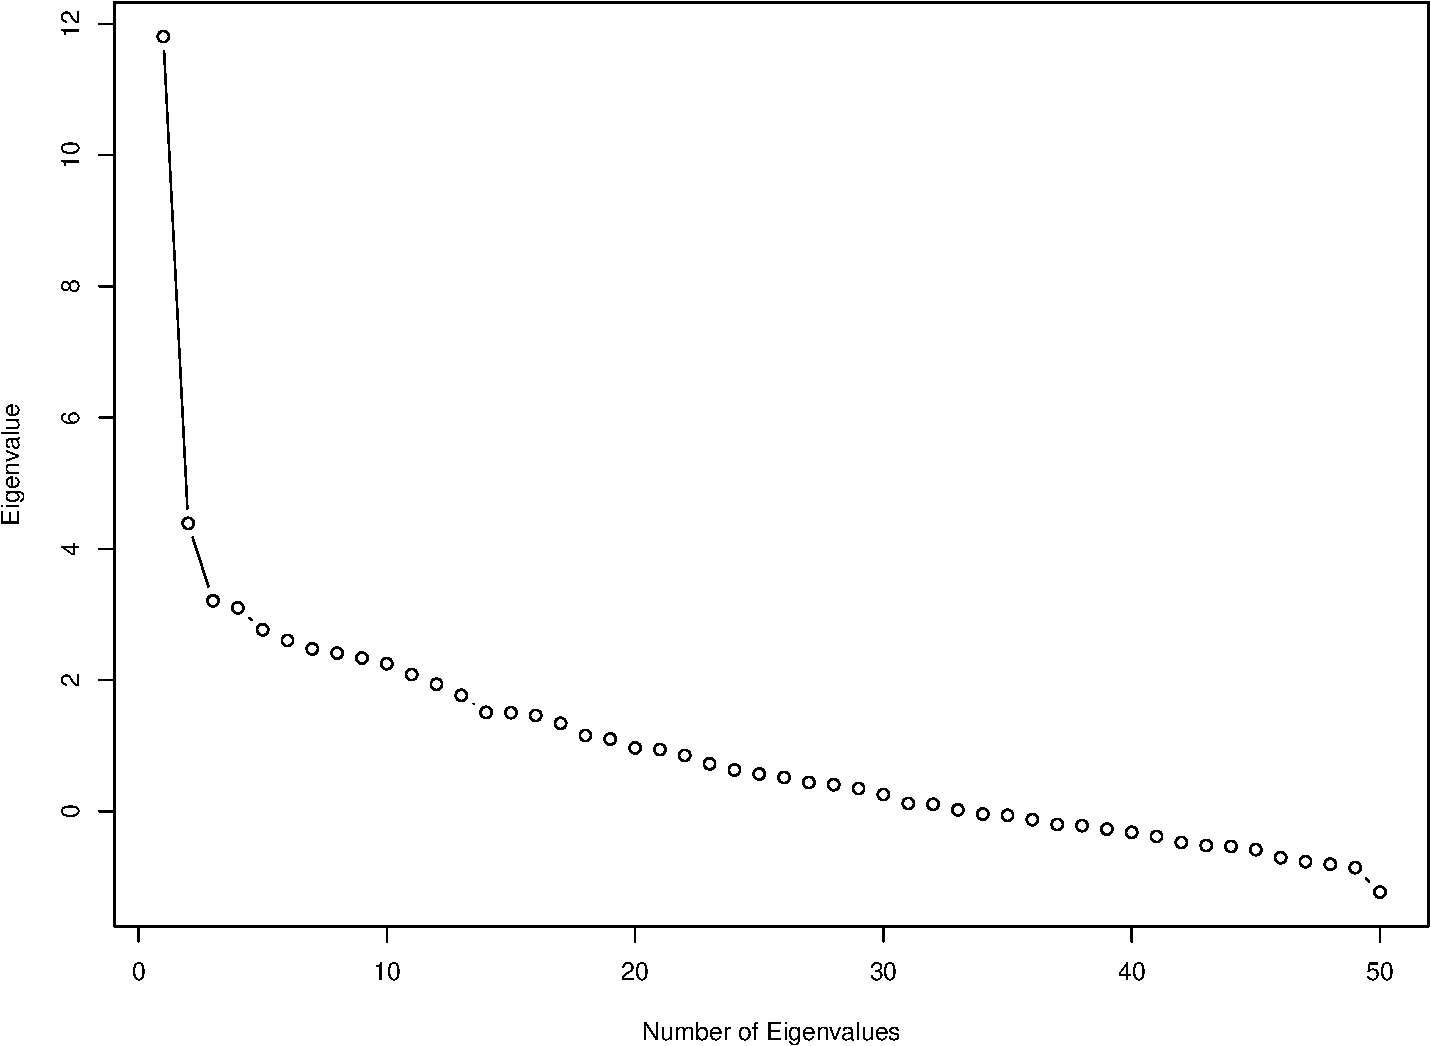
\includegraphics[keepaspectratio]{chap2_ItemTest_files/figure-pdf/unnamed-chunk-21-1.pdf}}

\section{多値への展開}\label{ux591aux5024ux3078ux306eux5c55ux958b}

\subsection{\texorpdfstring{\texttt{exametrika}における多値データ}{exametrikaにおける多値データ}}\label{exametrikaux306bux304aux3051ux308bux591aux5024ux30c7ux30fcux30bf}

\begin{itemize}
\tightlist
\item
  \texttt{exametrika}では多値データも扱えます

  \begin{itemize}
  \tightlist
  \item
    名義尺度データは\texttt{nominal};反応段階に順番性を考慮しないものです
  \item
    順序尺度データは\texttt{ordinal};3件法,5件法,7件法といった段階反応に対応します
  \item
    多肢選択(名義尺度水準)で正答反応を別途指定したものは\texttt{rated}
  \end{itemize}
\end{itemize}

\subsubsection{\texorpdfstring{\texttt{ordinal}なデータ}{ordinalなデータ}}\label{ordinalux306aux30c7ux30fcux30bf}

\begin{itemize}
\tightlist
\item
  サンプルデータで見てみましょう

  \begin{itemize}
  \tightlist
  \item
    \texttt{ordinal}データの例;J15S3810

    \begin{itemize}
    \tightlist
    \item
      データは\(U\)ではなく\(Q\)として入っています。
    \item
      欠測指示子行列は\(Z\)です。
    \end{itemize}
  \end{itemize}
\end{itemize}

\begin{Shaded}
\begin{Highlighting}[]
\NormalTok{dat }\OtherTok{\textless{}{-}}\NormalTok{ J15S3810}
\NormalTok{dat}\SpecialCharTok{$}\NormalTok{response.type}
\end{Highlighting}
\end{Shaded}

\begin{verbatim}
[1] "ordinal"
\end{verbatim}

\begin{Shaded}
\begin{Highlighting}[]
\NormalTok{dat}\SpecialCharTok{$}\NormalTok{Q }\SpecialCharTok{|\textgreater{}} \FunctionTok{head}\NormalTok{()}
\end{Highlighting}
\end{Shaded}

\begin{verbatim}
     V1 V2 V3 V4 V5 V6 V7 V8 V9 V10 V11 V12 V13 V14 V15
[1,]  2  2  3  0  3  1 -1 -1 -1  -1  -1  -1   1   2   2
[2,]  2  1  2 -1 -1 -1  2  1  3  -1  -1  -1   2   1   2
[3,]  3  2  2  2  3  3 -1 -1 -1  -1  -1  -1   3   3   2
[4,]  2  0  3 -1 -1 -1 -1 -1 -1   2   2   2   2   2   1
[5,]  2  2  1 -1 -1 -1  3  1  1  -1  -1  -1   2   1   3
[6,]  1  2  0  0  0  0 -1 -1 -1  -1  -1  -1   1   1   0
\end{verbatim}

\subsubsection{\texorpdfstring{\texttt{rated}なデータ}{ratedなデータ}}\label{ratedux306aux30c7ux30fcux30bf}

\begin{itemize}
\tightlist
\item
  サンプルデータで見てみましょう

  \begin{itemize}
  \tightlist
  \item
    \texttt{rated}データの例;J35S5000

    \begin{itemize}
    \tightlist
    \item
      データは\(Q\)として入っています
    \item
      欠測指示子行列は\(Z\)です
    \item
      変数\(CA\)に正答反応が入っています
    \item
      正答(1)か誤答(0)かを\(U\)に持っています
    \end{itemize}
  \end{itemize}
\end{itemize}

\begin{Shaded}
\begin{Highlighting}[]
\NormalTok{dat }\OtherTok{\textless{}{-}}\NormalTok{ J35S5000}
\NormalTok{dat}\SpecialCharTok{$}\NormalTok{response.type}
\end{Highlighting}
\end{Shaded}

\begin{verbatim}
[1] "rated"
\end{verbatim}

\begin{Shaded}
\begin{Highlighting}[]
\NormalTok{dat}\SpecialCharTok{$}\NormalTok{Q }\SpecialCharTok{|\textgreater{}} \FunctionTok{head}\NormalTok{(}\DecValTok{3}\NormalTok{)}
\end{Highlighting}
\end{Shaded}

\begin{verbatim}
     V1 V2 V3 V4 V5 V6 V7 V8 V9 V10 V11 V12 V13 V14 V15 V16 V17 V18 V19 V20 V21
[1,]  3  4 -1  5  3  5  3  2  3   1   3   1   2   5   4   5  -1   2   2   3   2
[2,]  1  4  4  3  3  5  3  2  2   3   3   6   1   4   3   5   1   2   2   4   4
[3,]  3  3  3  3  3  5  3  6  4   1   3   1   1   4   4   4   3   2   2   3   1
     V22 V23 V24 V25 V26 V27 V28 V29 V30 V31 V32 V33 V34 V35
[1,]   1   4   3   1   3   3   3   3   4   3   3   6   4   4
[2,]   2   3   2   3   1   5   5   2   4   3   1   4   2   3
[3,]   3   3   4   1   4   3   2   3   4   3   4   1   3   3
\end{verbatim}

\begin{Shaded}
\begin{Highlighting}[]
\NormalTok{dat}\SpecialCharTok{$}\NormalTok{CA}
\end{Highlighting}
\end{Shaded}

\begin{verbatim}
 [1] 3 3 3 3 2 5 3 4 4 4 3 6 2 4 4 5 1 2 3 1 1 1 3 4 3 4 3 2 2 4 3 4 5 2 1
\end{verbatim}

\begin{Shaded}
\begin{Highlighting}[]
\NormalTok{dat}\SpecialCharTok{$}\NormalTok{U }\SpecialCharTok{|\textgreater{}} \FunctionTok{head}\NormalTok{(}\DecValTok{3}\NormalTok{)}
\end{Highlighting}
\end{Shaded}

\begin{verbatim}
     [,1] [,2] [,3] [,4] [,5] [,6] [,7] [,8] [,9] [,10] [,11] [,12] [,13] [,14]
[1,]    1    0    0    0    0    1    1    0    0     0     1     0     1     0
[2,]    0    0    0    1    0    1    1    0    0     0     1     1     0     1
[3,]    1    1    1    1    0    1    1    0    1     0     1     0     0     1
     [,15] [,16] [,17] [,18] [,19] [,20] [,21] [,22] [,23] [,24] [,25] [,26]
[1,]     1     1     0     1     0     0     0     1     0     0     0     0
[2,]     0     1     1     1     0     0     0     0     1     0     1     0
[3,]     1     0     0     1     0     0     1     0     1     1     0     1
     [,27] [,28] [,29] [,30] [,31] [,32] [,33] [,34] [,35]
[1,]     1     0     0     1     1     0     0     0     0
[2,]     0     0     1     1     1     0     0     1     0
[3,]     1     1     0     1     1     1     0     0     0
\end{verbatim}

\begin{itemize}
\tightlist
\item
  自分でデータを作る時は,\texttt{response.type}を指定します

  \begin{itemize}
  \tightlist
  \item
    以下の例では\texttt{ltm}パッケージが必要です
  \end{itemize}
\end{itemize}

\begin{Shaded}
\begin{Highlighting}[]
\NormalTok{result4 }\OtherTok{\textless{}{-}} \FunctionTok{dataFormat}\NormalTok{(ltm}\SpecialCharTok{::}\NormalTok{Science[}\DecValTok{1}\SpecialCharTok{:}\DecValTok{5}\NormalTok{, ], }\AttributeTok{response.type =} \StringTok{"ordinal"}\NormalTok{)}
\NormalTok{result4}
\end{Highlighting}
\end{Shaded}

\begin{verbatim}
Response Type: ordinal 
Polytomous Response Pattern ( ordinal )
     Comfort Environment Work Future Technology Industry Benefit
[1,]       4           4    4      3          4        3       2
[2,]       3           4    3      3          3        3       3
[3,]       3           2    2      2          4        4       3
[4,]       3           3    2      2          4        4       3
[5,]       3           1    4      4          2        3       1

Missing Pattern
     Comfort Environment Work Future Technology Industry Benefit
[1,]       1           1    1      1          1        1       1
[2,]       1           1    1      1          1        1       1
[3,]       1           1    1      1          1        1       1
[4,]       1           1    1      1          1        1       1
[5,]       1           1    1      1          1        1       1

Weight
[1] 1 1 1 1 1 1 1
\end{verbatim}

\begin{itemize}
\tightlist
\item
  カテゴリラベルや反応段階も保持されます
\end{itemize}

\begin{Shaded}
\begin{Highlighting}[]
\NormalTok{result4}\SpecialCharTok{$}\NormalTok{ItemLabel}
\end{Highlighting}
\end{Shaded}

\begin{verbatim}
[1] "Comfort"     "Environment" "Work"        "Future"      "Technology" 
[6] "Industry"    "Benefit"    
\end{verbatim}

\begin{Shaded}
\begin{Highlighting}[]
\NormalTok{result4}\SpecialCharTok{$}\NormalTok{CategoryLabel[}\DecValTok{1}\NormalTok{]}
\end{Highlighting}
\end{Shaded}

\begin{verbatim}
$Comfort
[1] "strongly disagree" "disagree"          "agree"            
[4] "strongly agree"   
\end{verbatim}

\begin{itemize}
\tightlist
\item
  \texttt{response.type}のない多値データは\texttt{nominal}になります

  \begin{itemize}
  \tightlist
  \item
    以下の例では\texttt{psych}パッケージが必要です
  \end{itemize}
\end{itemize}

\begin{Shaded}
\begin{Highlighting}[]
\NormalTok{result5 }\OtherTok{\textless{}{-}} \FunctionTok{dataFormat}\NormalTok{(psych}\SpecialCharTok{::}\NormalTok{bfi[}\DecValTok{1}\SpecialCharTok{:}\DecValTok{5}\NormalTok{, }\DecValTok{1}\SpecialCharTok{:}\DecValTok{25}\NormalTok{])}
\NormalTok{result5}
\end{Highlighting}
\end{Shaded}

\begin{verbatim}
Response Type: nominal 
Polytomous Response Pattern ( nominal )
     A1 A2 A3 A4 A5 C1 C2 C3 C4 C5 E1 E2 E3 E4 E5 N1 N2 N3 N4 N5 O1 O2 O3 O4 O5
[1,]  2  4  3  4  4  2  3  3  4  4  3  3  3  4  4  3  4  2  2  3  3  6  3  4  3
[2,]  2  4  5  2  5  5  4  4  3  4  1  1  6  4  3  3  3  3  5  5  4  2  4  3  3
[3,]  5  4  5  4  4  4  5  4  2  5  2  4  4  4  5  4  5  4  2  3  4  2  5  5  2
[4,]  4  4  6  5  5  4  4  3  5  5  5  3  4  4  4  2  5  2  4  1  3  3  4  3  5
[5,]  2  3  3  4  5  4  4  5  3  2  2  2  5  4  5  2  3  4  4  3  3  3  4  3  3

Missing Pattern
     A1 A2 A3 A4 A5 C1 C2 C3 C4 C5 E1 E2 E3 E4 E5 N1 N2 N3 N4 N5 O1 O2 O3 O4 O5
[1,]  1  1  1  1  1  1  1  1  1  1  1  1  1  1  1  1  1  1  1  1  1  1  1  1  1
[2,]  1  1  1  1  1  1  1  1  1  1  1  1  1  1  1  1  1  1  1  1  1  1  1  1  1
[3,]  1  1  1  1  1  1  1  1  1  1  1  1  1  1  1  1  1  1  1  1  1  1  1  1  1
[4,]  1  1  1  1  1  1  1  1  1  1  1  1  1  1  1  1  1  1  1  1  1  1  1  1  1
[5,]  1  1  1  1  1  1  1  1  1  1  1  1  1  1  1  1  1  1  1  1  1  1  1  1  1

Weight
 [1] 1 1 1 1 1 1 1 1 1 1 1 1 1 1 1 1 1 1 1 1 1 1 1 1 1
\end{verbatim}

\begin{itemize}
\tightlist
\item
  正答(正しい選択肢)があるばあいは,引数\texttt{CA}で指定します
\end{itemize}

\begin{Shaded}
\begin{Highlighting}[]
\NormalTok{data3 }\OtherTok{\textless{}{-}} \FunctionTok{data.frame}\NormalTok{(}
    \AttributeTok{id =} \DecValTok{1}\SpecialCharTok{:}\DecValTok{5}\NormalTok{,}
    \AttributeTok{item1 =} \FunctionTok{c}\NormalTok{(}\DecValTok{1}\NormalTok{, }\ConstantTok{NA}\NormalTok{, }\DecValTok{2}\NormalTok{, }\DecValTok{4}\NormalTok{, }\DecValTok{1}\NormalTok{),}
    \AttributeTok{item2 =} \FunctionTok{c}\NormalTok{(}\DecValTok{1}\NormalTok{, }\DecValTok{3}\NormalTok{, }\DecValTok{2}\NormalTok{, }\DecValTok{4}\NormalTok{, }\DecValTok{5}\NormalTok{)}
\NormalTok{)}
\NormalTok{result6 }\OtherTok{\textless{}{-}} \FunctionTok{dataFormat}\NormalTok{(data3, }\AttributeTok{CA =} \FunctionTok{c}\NormalTok{(}\DecValTok{4}\NormalTok{, }\DecValTok{2}\NormalTok{))}
\NormalTok{result6}
\end{Highlighting}
\end{Shaded}

\begin{verbatim}
Response Type: rated 
Polytomous Response Pattern ( rated )
     item1 item2
[1,]     1     1
[2,]    -1     3
[3,]     2     2
[4,]     4     4
[5,]     1     5

Correct Answers
[1] 4 2

Missing Pattern
     item1 item2
[1,]     1     1
[2,]     0     1
[3,]     1     1
[4,]     1     1
[5,]     1     1

Weight
[1] 1 1
\end{verbatim}

\begin{Shaded}
\begin{Highlighting}[]
\NormalTok{result6}\SpecialCharTok{$}\NormalTok{U}
\end{Highlighting}
\end{Shaded}

\begin{verbatim}
     [,1] [,2]
[1,]    0    0
[2,]    0    0
[3,]    0    1
[4,]    1    0
[5,]    0    0
\end{verbatim}

\subsection{項目分析をしよう(多値データの場合)}\label{ux9805ux76eeux5206ux6790ux3092ux3057ux3088ux3046ux591aux5024ux30c7ux30fcux30bfux306eux5834ux5408}

\begin{itemize}
\tightlist
\item
  サンプルデータ\texttt{J5S1000}を例に見てみましょう
\end{itemize}

\begin{Shaded}
\begin{Highlighting}[]
\NormalTok{dat }\OtherTok{\textless{}{-}}\NormalTok{ J5S1000}
\FunctionTok{TestStatistics}\NormalTok{(dat)}
\end{Highlighting}
\end{Shaded}

\begin{verbatim}
Test Statistics
                   value
SampleSize 1000.00000000
TestLength    5.00000000
Median       12.00000000
Max          18.00000000
Min           4.00000000
Range        14.00000000
Mean         11.45700000
SD            2.92107578
Skewness     -0.08836075
Kurtosis     -0.55776379
Alpha         0.59462241
\end{verbatim}

\subsection{まとめて分析(項目分析・多値データの場合)}\label{ux307eux3068ux3081ux3066ux5206ux6790ux9805ux76eeux5206ux6790ux591aux5024ux30c7ux30fcux30bfux306eux5834ux5408}

\begin{Shaded}
\begin{Highlighting}[]
\FunctionTok{ItemStatistics}\NormalTok{(dat)}
\end{Highlighting}
\end{Shaded}

\begin{verbatim}
Item Statistics
  ItemLabel  NR Entropy Threshold.1 Threshold.2 Threshold.3 ITCrr
1        V1 993   0.991      -0.805      0.0290       0.805 0.670
2        V2 990   0.964      -0.580      0.6697          NA 0.635
3        V3 996   0.995      -0.832     -0.0403       0.665 0.675
4        V4 997   0.970      -0.638      0.5803          NA 0.679
5        V5 998   0.996      -0.714      0.0126       0.795 0.686
\end{verbatim}

\subsection{まとめて分析(項目間分析・多値データの場合)}\label{ux307eux3068ux3081ux3066ux5206ux6790ux9805ux76eeux9593ux5206ux6790ux591aux5024ux30c7ux30fcux30bfux306eux5834ux5408}

\begin{Shaded}
\begin{Highlighting}[]
\NormalTok{IIAnalysis }\OtherTok{\textless{}{-}} \FunctionTok{InterItemAnalysis}\NormalTok{(dat)}
\NormalTok{IIAnalysis}\SpecialCharTok{$}\NormalTok{JSS}
\end{Highlighting}
\end{Shaded}

\begin{verbatim}
    V1  V2  V3  V4  V5
V1 993 983 989 990 991
V2 983 990 986 987 988
V3 989 986 996 993 994
V4 990 987 993 997 995
V5 991 988 994 995 998
\end{verbatim}

\subsubsection{同時選択率(Joint Selection
Ratio)}\label{ux540cux6642ux9078ux629eux7387joint-selection-ratio}

\begin{itemize}
\tightlist
\item
  同時選択率Joint Selection
  Ratioは\texttt{JSR}変数にリストとして入っています

  \begin{itemize}
  \tightlist
  \item
    項目\(J\)と項目\(K\)の同時選択率行列は\texttt{JSR{[}{[}J{]}{]}{[}{[}K{]}{]}}で表示します
  \end{itemize}
\end{itemize}

\begin{Shaded}
\begin{Highlighting}[]
\NormalTok{IIAnalysis}\SpecialCharTok{$}\NormalTok{JSR[[}\DecValTok{1}\NormalTok{]][[}\DecValTok{2}\NormalTok{]]}
\end{Highlighting}
\end{Shaded}

\begin{verbatim}
         
             V2-Cat1    V2-Cat2    V2-Cat3
  V1-Cat1 0.09053917 0.08443540 0.03560529
  V1-Cat2 0.07934893 0.16073245 0.06103764
  V1-Cat3 0.07222787 0.13326551 0.07426246
  V1-Cat4 0.03865717 0.08952187 0.08036623
\end{verbatim}

\subsubsection{条件付き選択率(Conditional Selection
Ratio)}\label{ux6761ux4ef6ux4ed8ux304dux9078ux629eux7387conditional-selection-ratio}

\begin{itemize}
\tightlist
\item
  同時選択率Conditional Selection
  Ratioは\texttt{CSR}変数にリストとして入っています

  \begin{itemize}
  \tightlist
  \item
    項目\(J\)と項目\(K\)の同時選択率行列は\texttt{CSR{[}{[}J{]}{]}{[}{[}K{]}{]}}で表示します
  \end{itemize}
\end{itemize}

\begin{Shaded}
\begin{Highlighting}[]
\NormalTok{IIAnalysis}\SpecialCharTok{$}\NormalTok{CSR[[}\DecValTok{1}\NormalTok{]][[}\DecValTok{2}\NormalTok{]]}
\end{Highlighting}
\end{Shaded}

\begin{verbatim}
          V2-Cat1   V2-Cat2   V2-Cat3
V1-Cat1 0.4299517 0.4009662 0.1690821
V1-Cat2 0.2635135 0.5337838 0.2027027
V1-Cat3 0.2581818 0.4763636 0.2654545
V1-Cat4 0.1853659 0.4292683 0.3853659
\end{verbatim}

\subsubsection{項目情報量}\label{ux9805ux76eeux60c5ux5831ux91cf-1}

\begin{Shaded}
\begin{Highlighting}[]
\NormalTok{IIAnalysis}\SpecialCharTok{$}\NormalTok{MI}
\end{Highlighting}
\end{Shaded}

\begin{verbatim}
           [,1]       [,2]       [,3]       [,4]       [,5]
[1,]        NaN 0.03668416 0.03935180 0.04826507 0.04651449
[2,] 0.03668416        NaN 0.03870059 0.08680066 0.04694270
[3,] 0.03935180 0.03870059        NaN 0.06223498 0.03452874
[4,] 0.04826507 0.08680066 0.06223498        NaN 0.04703299
[5,] 0.04651449 0.04694270 0.03452874 0.04703299        NaN
\end{verbatim}

\subsection{多分相関係数(Polychoric
correlation)}\label{ux591aux5206ux76f8ux95a2ux4fc2ux6570polychoric-correlation}

\begin{Shaded}
\begin{Highlighting}[]
\NormalTok{IIAnalysis}\SpecialCharTok{$}\NormalTok{Polychoric}
\end{Highlighting}
\end{Shaded}

\begin{verbatim}
          [,1]      [,2]      [,3]      [,4]      [,5]
[1,] 1.0000000 0.2456614 0.2452777 0.2906536 0.2766477
[2,] 0.2456614 1.0000000 0.2557499 0.4055239 0.2831192
[3,] 0.2452777 0.2557499 1.0000000 0.3237882 0.2087904
[4,] 0.2906536 0.4055239 0.3237882 1.0000000 0.2942858
[5,] 0.2766477 0.2831192 0.2087904 0.2942858 1.0000000
\end{verbatim}

\subsection{次元性分析(多分相関係数の固有値分解)}\label{ux6b21ux5143ux6027ux5206ux6790ux591aux5206ux76f8ux95a2ux4fc2ux6570ux306eux56faux6709ux5024ux5206ux89e3}

\begin{Shaded}
\begin{Highlighting}[]
\FunctionTok{Dimensionality}\NormalTok{(dat)}
\end{Highlighting}
\end{Shaded}

\begin{verbatim}
Dimensionality Analyeis
Eigenvalues
[1] 2.1397364 0.8040388 0.7746611 0.6995033 0.5820604
Percentage Of Variance
[1] 42.79473 16.08078 15.49322 13.99007 11.64121
Cummurative Percentage
[1]  42.79473  58.87550  74.36873  88.35879 100.00000
\end{verbatim}

\pandocbounded{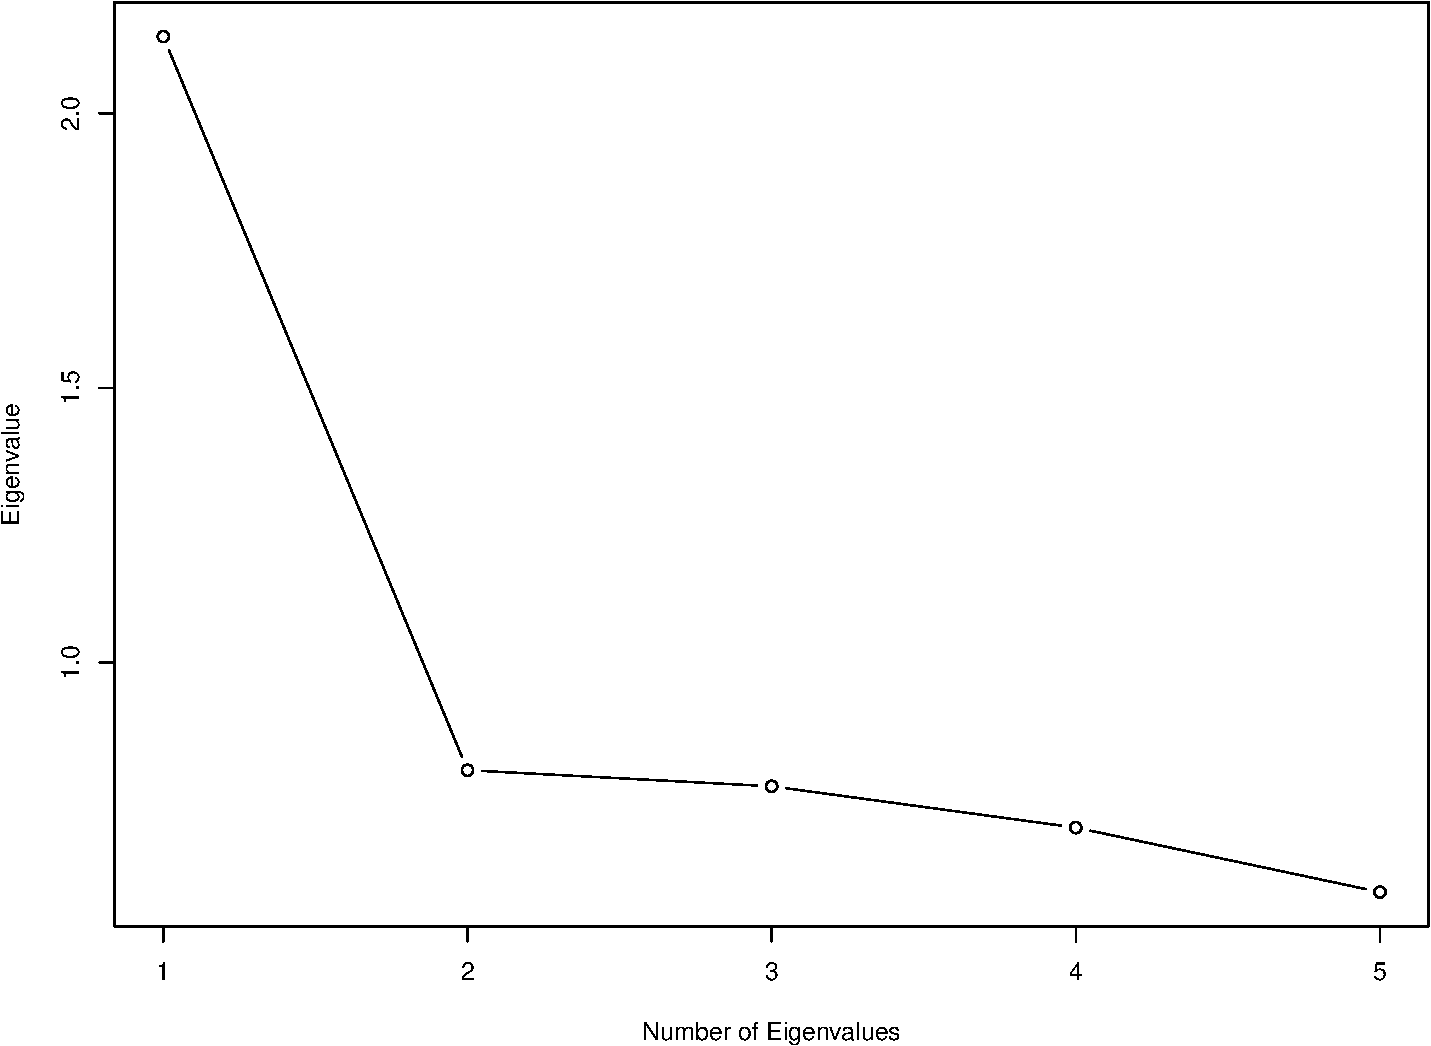
\includegraphics[keepaspectratio]{chap2_ItemTest_files/figure-pdf/unnamed-chunk-35-1.pdf}}

\bookmarksetup{startatroot}

\chapter{Rをつかった項目反応理論の実習}\label{rux3092ux3064ux304bux3063ux305fux9805ux76eeux53cdux5fdcux7406ux8ad6ux306eux5b9fux7fd2}

\section{準備しましょう}\label{ux6e96ux5099ux3057ux307eux3057ux3087ux3046-1}

\subsection{サンプルデータを用います}\label{ux30b5ux30f3ux30d7ux30ebux30c7ux30fcux30bfux3092ux7528ux3044ux307eux3059}

\begin{itemize}
\tightlist
\item
  RStudioでプロジェクトを開いているか確認してくださいね
\item
  \texttt{exametrika}が持っている\texttt{J15S500}を例に
\end{itemize}

\begin{Shaded}
\begin{Highlighting}[]
\FunctionTok{library}\NormalTok{(exametrika)}
\end{Highlighting}
\end{Shaded}

\begin{verbatim}
Loading required package: mvtnorm
\end{verbatim}

\begin{verbatim}
Loading required package: igraph
\end{verbatim}

\begin{verbatim}

Attaching package: 'igraph'
\end{verbatim}

\begin{verbatim}
The following objects are masked from 'package:stats':

    decompose, spectrum
\end{verbatim}

\begin{verbatim}
The following object is masked from 'package:base':

    union
\end{verbatim}

\begin{Shaded}
\begin{Highlighting}[]
\NormalTok{dat }\OtherTok{\textless{}{-}}\NormalTok{ J15S500}
\NormalTok{dat}\SpecialCharTok{$}\NormalTok{U }\SpecialCharTok{|\textgreater{}} \FunctionTok{head}\NormalTok{()}
\end{Highlighting}
\end{Shaded}

\begin{verbatim}
     Item01 Item02 Item03 Item04 Item05 Item06 Item07 Item08 Item09 Item10
[1,]      0      1      1      0      1      1      0      0      0      1
[2,]      1      1      1      1      1      1      0      1      0      1
[3,]      1      1      1      1      1      1      0      0      0      1
[4,]      1      1      1      1      1      1      1      1      0      0
[5,]      1      1      0      1      1      0      0      0      0      1
[6,]      1      1      1      1      1      1      1      1      0      0
     Item11 Item12 Item13 Item14 Item15
[1,]      1      0      1      0      1
[2,]      0      0      1      0      1
[3,]      0      0      1      1      1
[4,]      0      1      1      1      0
[5,]      0      0      0      1      0
[6,]      1      0      1      1      1
\end{verbatim}

\section{実行しちゃいましょう}\label{ux5b9fux884cux3057ux3061ux3083ux3044ux307eux3057ux3087ux3046}

\begin{itemize}
\tightlist
\item
  何やら色々出てきますので,順次解説していきます
\end{itemize}

\begin{Shaded}
\begin{Highlighting}[]
\NormalTok{result }\OtherTok{\textless{}{-}} \FunctionTok{IRT}\NormalTok{(dat)}
\end{Highlighting}
\end{Shaded}

\begin{verbatim}

iter 1 LogLik -3915.61 
iter 2 LogLik -3901.1 
iter 3 LogLik -3896.89 
iter 4
LogLik -3894.98 
iter 5 LogLik -3894.02 
iter 6 LogLik -3893.53 
iter 7 LogLik
-3893.28 
iter 8 LogLik -3893.15 
iter 9 LogLik -3893.08 
iter 10 LogLik -3893.04

iter 11 LogLik -3893.03
\end{verbatim}

\begin{Shaded}
\begin{Highlighting}[]
\NormalTok{result}
\end{Highlighting}
\end{Shaded}

\begin{verbatim}
Item Parameters
       slope location PSD(slope) PSD(location)
Item01 0.698   -1.683     0.1093         0.266
Item02 0.810   -1.552     0.1166         0.221
Item03 0.559   -1.838     0.0988         0.338
Item04 1.416   -1.178     0.1569         0.113
Item05 0.681   -2.242     0.1152         0.360
Item06 0.997   -2.162     0.1499         0.273
Item07 1.084   -1.039     0.1281         0.130
Item08 0.694   -0.558     0.1002         0.153
Item09 0.347    1.630     0.0766         0.427
Item10 0.492   -1.421     0.0907         0.306
Item11 1.122    1.020     0.1314         0.124
Item12 1.216    1.031     0.1385         0.117
Item13 0.875   -0.720     0.1111         0.133
Item14 1.200   -1.232     0.1407         0.134
Item15 0.823   -1.203     0.1127         0.180

Item Fit Indices
       model_log_like bench_log_like null_log_like model_Chi_sq null_Chi_sq
Item01       -263.524       -240.190      -283.343       46.669      86.307
Item02       -252.914       -235.436      -278.949       34.954      87.025
Item03       -281.083       -260.906      -293.598       40.353      65.383
Item04       -205.851       -192.072      -265.962       27.558     147.780
Item05       -232.072       -206.537      -247.403       51.070      81.732
Item06       -173.930       -153.940      -198.817       39.981      89.755
Item07       -252.039       -228.379      -298.345       47.320     139.933
Item08       -313.754       -293.225      -338.789       41.057      91.127
Item09       -325.692       -300.492      -327.842       50.399      54.700
Item10       -309.448       -288.198      -319.850       42.500      63.303
Item11       -250.836       -224.085      -299.265       53.501     150.360
Item12       -240.247       -214.797      -293.598       50.900     157.603
Item13       -291.816       -262.031      -328.396       59.571     132.730
Item14       -224.330       -204.953      -273.212       38.754     136.519
Item15       -273.120       -254.764      -302.847       36.713      96.166
       model_df null_df   NFI   RFI   IFI   TLI   CFI RMSEA    AIC    CAIC
Item01       12      13 0.459 0.414 0.533 0.488 0.527 0.076 22.669 -27.930
Item02       12      13 0.598 0.565 0.694 0.664 0.690 0.062 10.954 -39.645
Item03       12      13 0.383 0.331 0.469 0.414 0.459 0.069 16.353 -34.246
Item04       12      13 0.814 0.798 0.885 0.875 0.885 0.051  3.558 -47.041
Item05       12      13 0.375 0.323 0.440 0.384 0.432 0.081 27.070 -23.529
Item06       12      13 0.555 0.517 0.640 0.605 0.635 0.068 15.981 -34.619
Item07       12      13 0.662 0.634 0.724 0.699 0.722 0.077 23.320 -27.279
Item08       12      13 0.549 0.512 0.633 0.597 0.628 0.070 17.057 -33.542
Item09       12      13 0.079 0.002 0.101 0.002 0.079 0.080 26.399 -24.201
Item10       12      13 0.329 0.273 0.405 0.343 0.394 0.071 18.500 -32.099
Item11       12      13 0.644 0.615 0.700 0.673 0.698 0.083 29.501 -21.099
Item12       12      13 0.677 0.650 0.733 0.709 0.731 0.081 26.900 -23.699
Item13       12      13 0.551 0.514 0.606 0.570 0.603 0.089 35.571 -15.028
Item14       12      13 0.716 0.692 0.785 0.765 0.783 0.067 14.754 -35.846
Item15       12      13 0.618 0.586 0.706 0.678 0.703 0.064 12.713 -37.886
           BIC
Item01 -27.906
Item02 -39.621
Item03 -34.222
Item04 -47.017
Item05 -23.505
Item06 -34.595
Item07 -27.255
Item08 -33.518
Item09 -24.177
Item10 -32.076
Item11 -21.075
Item12 -23.675
Item13 -15.004
Item14 -35.822
Item15 -37.862

Model Fit Indices
                   value
model_log_like -3890.655
bench_log_like -3560.005
null_log_like  -4350.217
model_Chi_sq     661.300
null_Chi_sq     1580.424
model_df         180.000
null_df          195.000
NFI                0.582
RFI                0.547
IFI                0.656
TLI                0.624
CFI                0.653
RMSEA              0.073
AIC              301.300
CAIC            -457.689
BIC             -457.330
\end{verbatim}

\section{モデル適合度}\label{ux30e2ux30c7ux30ebux9069ux5408ux5ea6}

\begin{itemize}
\tightlist
\item
  尤度Likelihoodとは,観測されたデータが特定のパラメータを持つモデルから生成された可能性を表します。\([0,1]\)の範囲にあって,\(1\)に近いほど「ありえそう」であることを表します。
\item
  対数尤度Log-likelihoodとは,その対数をとったものです。

  \begin{itemize}
  \tightlist
  \item
    尤度の計算は非常に小さな桁数まで重要なので,計算の精度を保つために対数を取ります
  \end{itemize}
\item
  対数尤度の範囲は\((-\inf,0]\)で,\(0\)に近いほど「ありえそう」であることを表します。
\end{itemize}

\subsection{モデルの評価}\label{ux30e2ux30c7ux30ebux306eux8a55ux4fa1}

\begin{itemize}
\tightlist
\item
  モデルを評価する時に,「データにバッチリ完璧に当てはまってるぜモデル」と「データなんか関係ない完璧に当てはまってないモデル」を考えます
\item
  前者を飽和モデル(saturated model),後者をヌルモデル(null
  model)といいます
\item
  飽和モデルの代わりに,実質的な飽和モデル/ベンチマークになるモデルと比較することもあります
\item
  実際に推定したモデルはこの量モデルの間のどこかに入るはずですね
\end{itemize}

\begin{figure}[H]

{\centering \pandocbounded{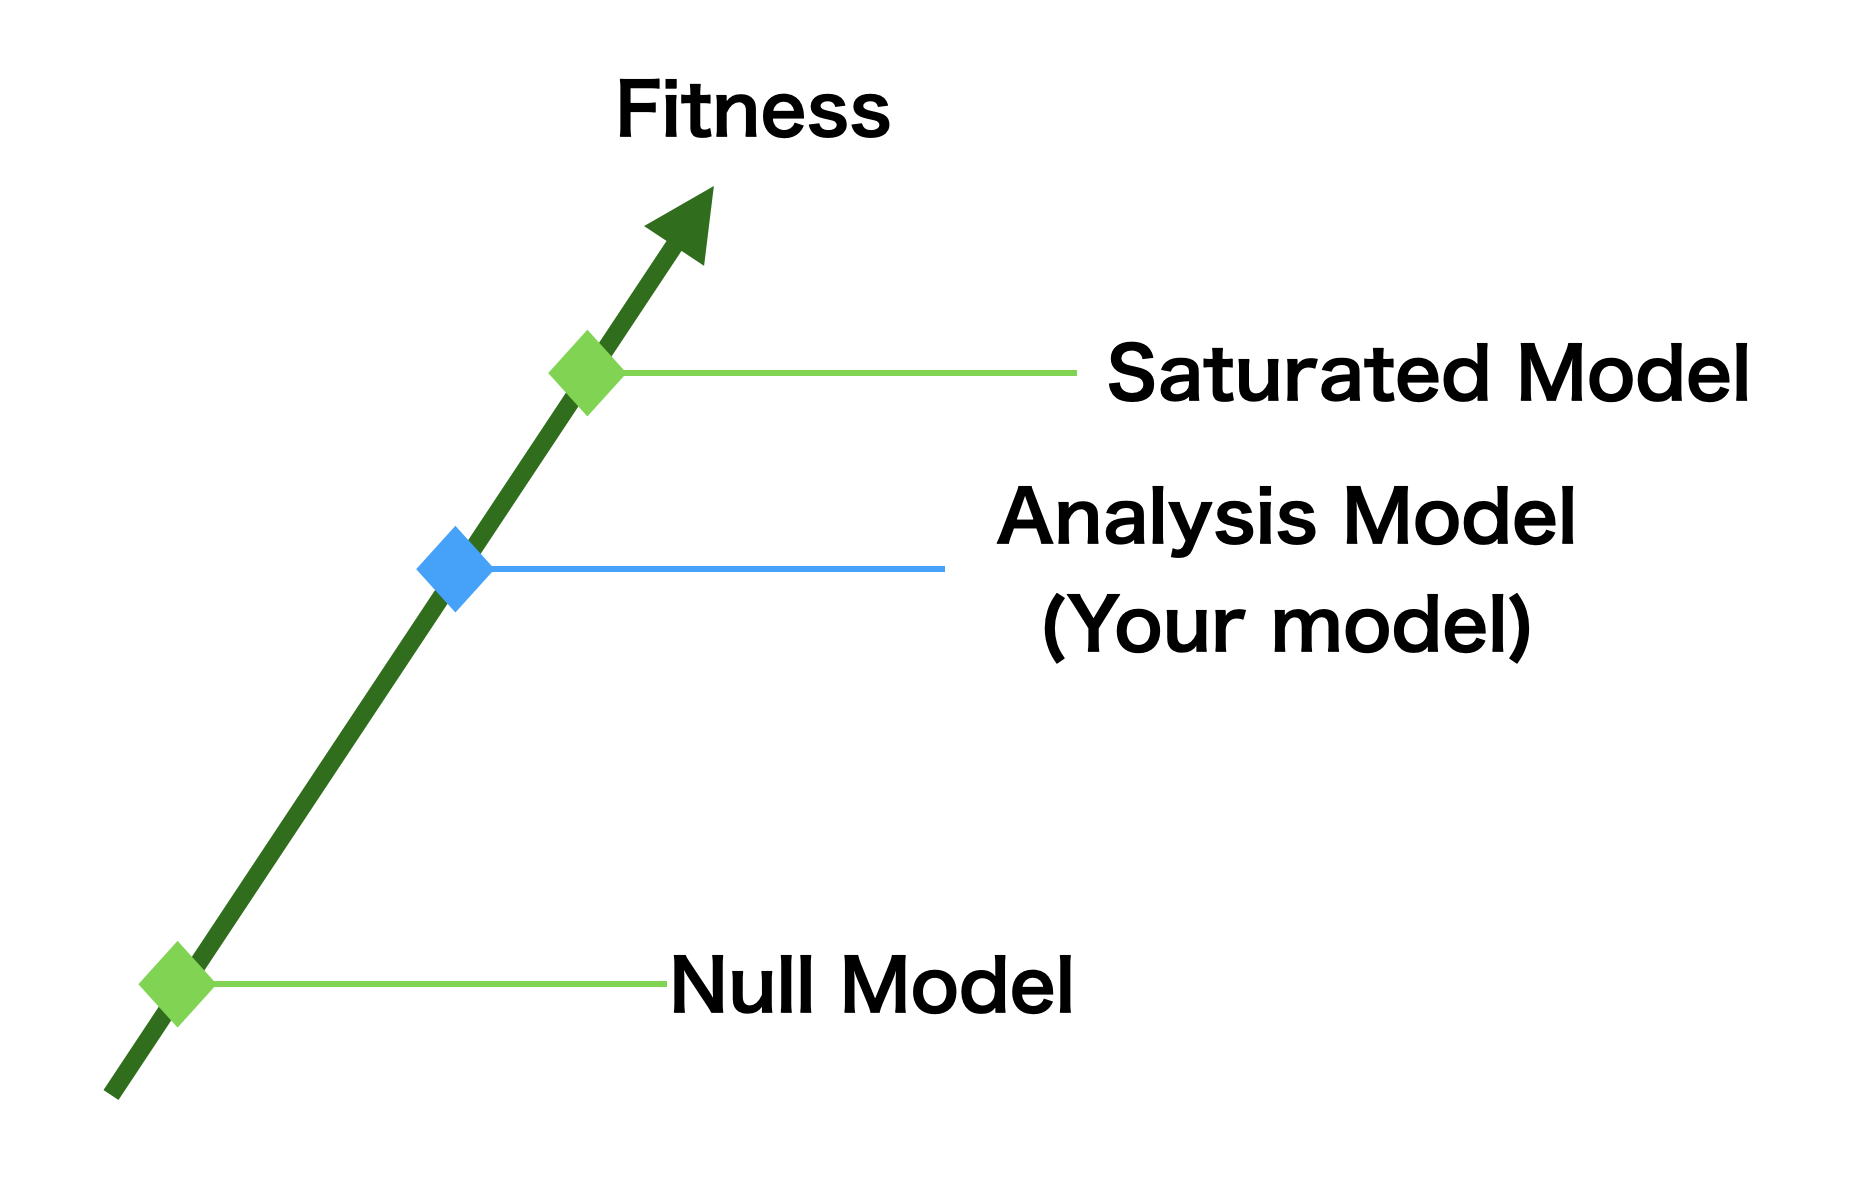
\includegraphics[keepaspectratio]{modelFItinSEM.png}}

}

\caption{Test Data Enginieering,P.139}

\end{figure}%

\begin{itemize}
\tightlist
\item
  カイ二乗(Chi-square,\(\chi^2\))値は,対数尤度に変換した後のモデル間の距離と考えることができます
\end{itemize}

\begin{figure}[H]

{\centering \pandocbounded{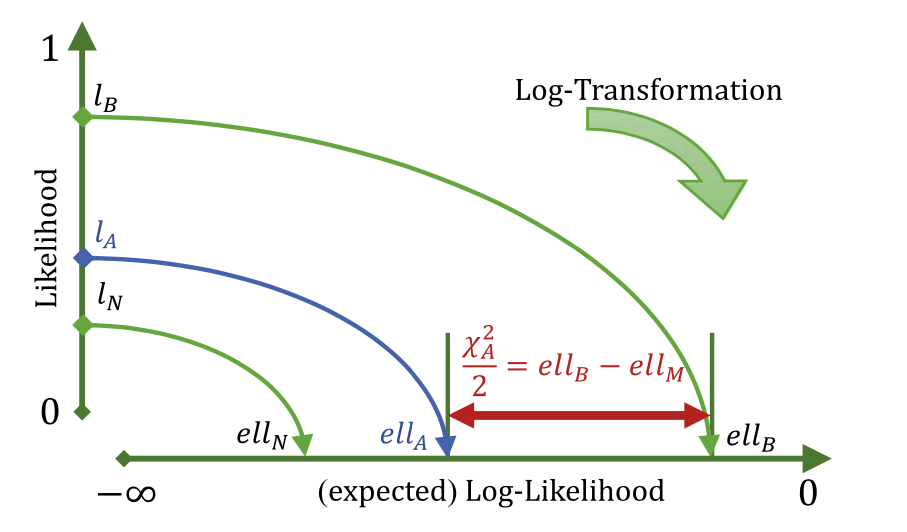
\includegraphics[keepaspectratio]{ChisqTransFormation.png}}

}

\caption{Test Data Engineering,P.144}

\end{figure}%

\begin{itemize}
\tightlist
\item
  SEMで用いられる標準化された指標は,カイ二乗値を変換・標準化して表現したものです
\item
  \texttt{exametrika}ではこれらの指標を適合度として表示します
\end{itemize}

\begin{figure}[H]

{\centering \pandocbounded{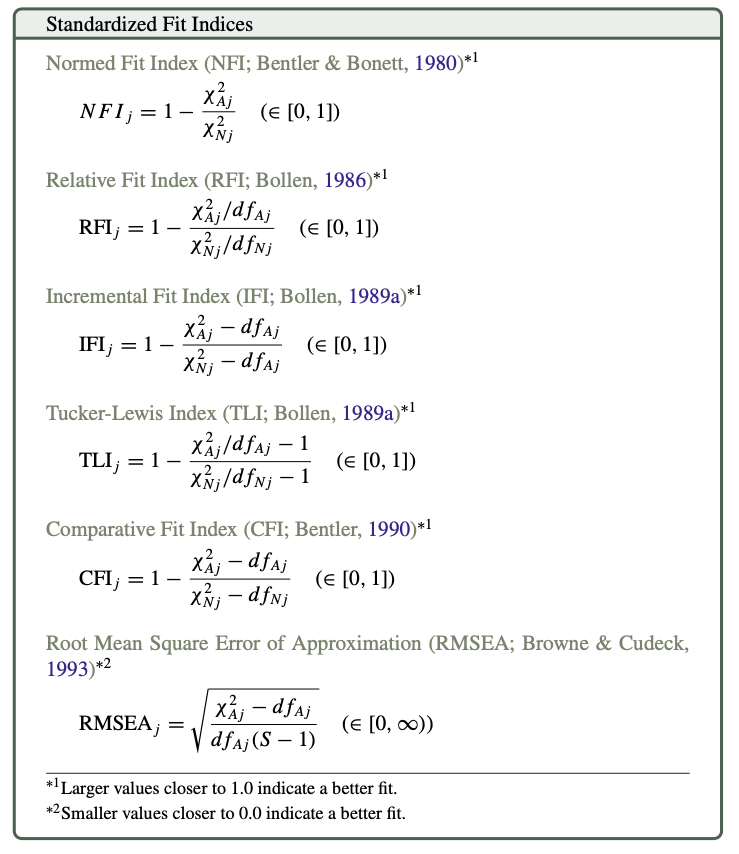
\includegraphics[keepaspectratio]{otherIndices.png}}

}

\caption{Test Data Enginieering,P.148}

\end{figure}%

\begin{itemize}
\tightlist
\item
  情報量基準も同様に,カイ二乗値に基づいて考えることができます
\end{itemize}

\begin{figure}[H]

{\centering \pandocbounded{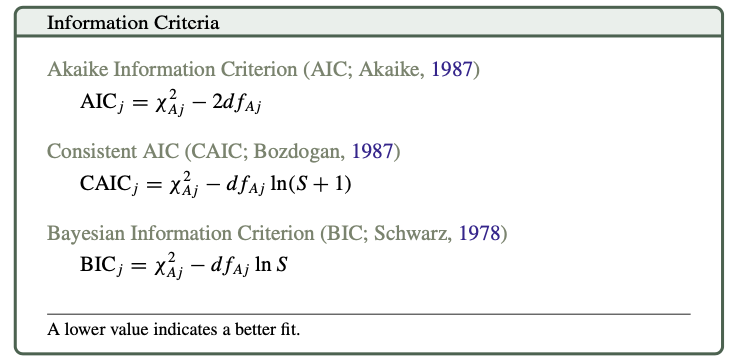
\includegraphics[keepaspectratio]{InformationCriteria.png}}

}

\caption{Test Data Engineering,P.150}

\end{figure}%

\subsection{改めて確認してみましょう}\label{ux6539ux3081ux3066ux78baux8a8dux3057ux3066ux307fux307eux3057ux3087ux3046}

\begin{itemize}
\tightlist
\item
  \texttt{TestFitIndices}でテスト全体の適合度指標にアクセスできます。
\end{itemize}

\begin{Shaded}
\begin{Highlighting}[]
\NormalTok{result}\SpecialCharTok{$}\NormalTok{TestFitIndices}
\end{Highlighting}
\end{Shaded}

\begin{verbatim}
  model_log_like bench_log_like null_log_like model_Chi_sq null_Chi_sq model_df
1      -3890.655      -3560.005     -4350.217     661.2999    1580.424      180
  null_df      NFI       RFI       IFI       TLI       CFI      RMSEA      AIC
1     195 0.581568 0.5466987 0.6563184 0.6236472 0.6525974 0.07320173 301.2999
       CAIC       BIC
1 -457.6892 -457.3296
\end{verbatim}

\begin{itemize}
\tightlist
\item
  \texttt{ItemFitIndices}で項目ごとの適合度指標にアクセスできます。
\end{itemize}

\begin{Shaded}
\begin{Highlighting}[]
\NormalTok{result}\SpecialCharTok{$}\NormalTok{ItemFitIndices}
\end{Highlighting}
\end{Shaded}

\begin{verbatim}
       model_log_like bench_log_like null_log_like model_Chi_sq null_Chi_sq
Item01      -263.5243      -240.1896     -283.3432     46.66935    86.30724
Item02      -252.9135      -235.4364     -278.9486     34.95429    87.02454
Item03      -281.0830      -260.9064     -293.5981     40.35320    65.38341
Item04      -205.8510      -192.0718     -265.9618     27.55847   147.77999
Item05      -232.0722      -206.5372     -247.4032     51.06994    81.73195
Item06      -173.9301      -153.9397     -198.8174     39.98071    89.75530
Item07      -252.0388      -228.3788     -298.3455     47.32008   139.93348
Item08      -313.7538      -293.2252     -338.7888     41.05727    91.12723
Item09      -325.6916      -300.4923     -327.8422     50.39860    54.69970
Item10      -309.4483      -288.1984     -319.8497     42.49979    63.30265
Item11      -250.8358      -224.0855     -299.2653     53.50067   150.35960
Item12      -240.2466      -214.7967     -293.5981     50.89987   157.60288
Item13      -291.8161      -262.0307     -328.3959     59.57087   132.73044
Item14      -224.3296      -204.9528     -273.2123     38.75364   136.51897
Item15      -273.1202      -254.7637     -302.8469     36.71311    96.16648
       model_df null_df        NFI         RFI       IFI         TLI        CFI
Item01       12      13 0.45926499 0.414203743 0.5334325 0.487656904 0.52706791
Item02       12      13 0.59833988 0.564868207 0.6940430 0.664068918 0.68990977
Item03       12      13 0.38282212 0.331390625 0.4688763 0.413631891 0.45873713
Item04       12      13 0.81351690 0.797976644 0.8854141 0.874944274 0.88456394
Item05       12      13 0.37515325 0.323082692 0.4397125 0.384190733 0.43156068
Item06       12      13 0.55455873 0.517438625 0.6401440 0.605076904 0.63545560
Item07       12      13 0.66183875 0.633658645 0.7239184 0.698555334 0.72174339
Item08       12      13 0.54945112 0.511905385 0.6327779 0.597084005 0.62807754
Item09       12      13 0.07863106 0.001850314 0.1007289 0.002427154 0.07916353
Item10       12      13 0.32862538 0.272677499 0.4054929 0.343147103 0.39367425
Item11       12      13 0.64418187 0.614530359 0.7000521 0.672690798 0.69786843
Item12       12      13 0.67703716 0.650123586 0.7328358 0.708570602 0.73098825
Item13       12      13 0.55118908 0.513788174 0.6059745 0.569573873 0.60268358
Item14       12      13 0.71613001 0.692474173 0.7851441 0.765354997 0.78340461
Item15       12      13 0.61823376 0.586419908 0.7063782 0.678084951 0.70284765
            RMSEA      AIC      CAIC       BIC
Item01 0.07609076 22.66935 -27.92993 -27.90595
Item02 0.06191430 10.95429 -39.64499 -39.62101
Item03 0.06881136 16.35320 -34.24608 -34.22210
Item04 0.05097328  3.55847 -47.04080 -47.01683
Item05 0.08077566 27.06994 -23.52933 -23.50535
Item06 0.06835787 15.98071 -34.61856 -34.59458
Item07 0.07680154 23.32008 -27.27919 -27.25522
Item08 0.06966049 17.05727 -33.54200 -33.51802
Item09 0.08007866 26.39860 -24.20067 -24.17669
Item10 0.07136866 18.49979 -32.09948 -32.07551
Item11 0.08325047 29.50067 -21.09860 -21.07463
Item12 0.08059966 26.89987 -23.69940 -23.67542
Item13 0.08913118 35.57087 -15.02840 -15.00443
Item14 0.06684217 14.75364 -35.84563 -35.82166
Item15 0.06424256 12.71311 -37.88616 -37.86218
\end{verbatim}

\subsection{可視化しましょう}\label{ux53efux8996ux5316ux3057ux307eux3057ux3087ux3046}

\begin{itemize}
\tightlist
\item
  項目反応関数(IRF)を表示してみましょう

  \begin{itemize}
  \tightlist
  \item
    表示させたい項目を\texttt{items}オプションで与えます
  \item
    表示させたい図の種類を\texttt{type}オプションで指定します

    \begin{itemize}
    \tightlist
    \item
      \texttt{IRF},\texttt{TRF},\texttt{IIC},\texttt{TIC}を選ぶことができます。
    \item
      \texttt{ICC}(Item Characteristic
      Curve)も可(\texttt{IRF}と同じです)
    \end{itemize}
  \item
    指定しなければ全ての項目をプロットします
  \end{itemize}
\end{itemize}

\begin{Shaded}
\begin{Highlighting}[]
\FunctionTok{plot}\NormalTok{(result, }\AttributeTok{items =} \DecValTok{1}\NormalTok{, }\AttributeTok{type =} \StringTok{"IRF"}\NormalTok{)}
\end{Highlighting}
\end{Shaded}

\pandocbounded{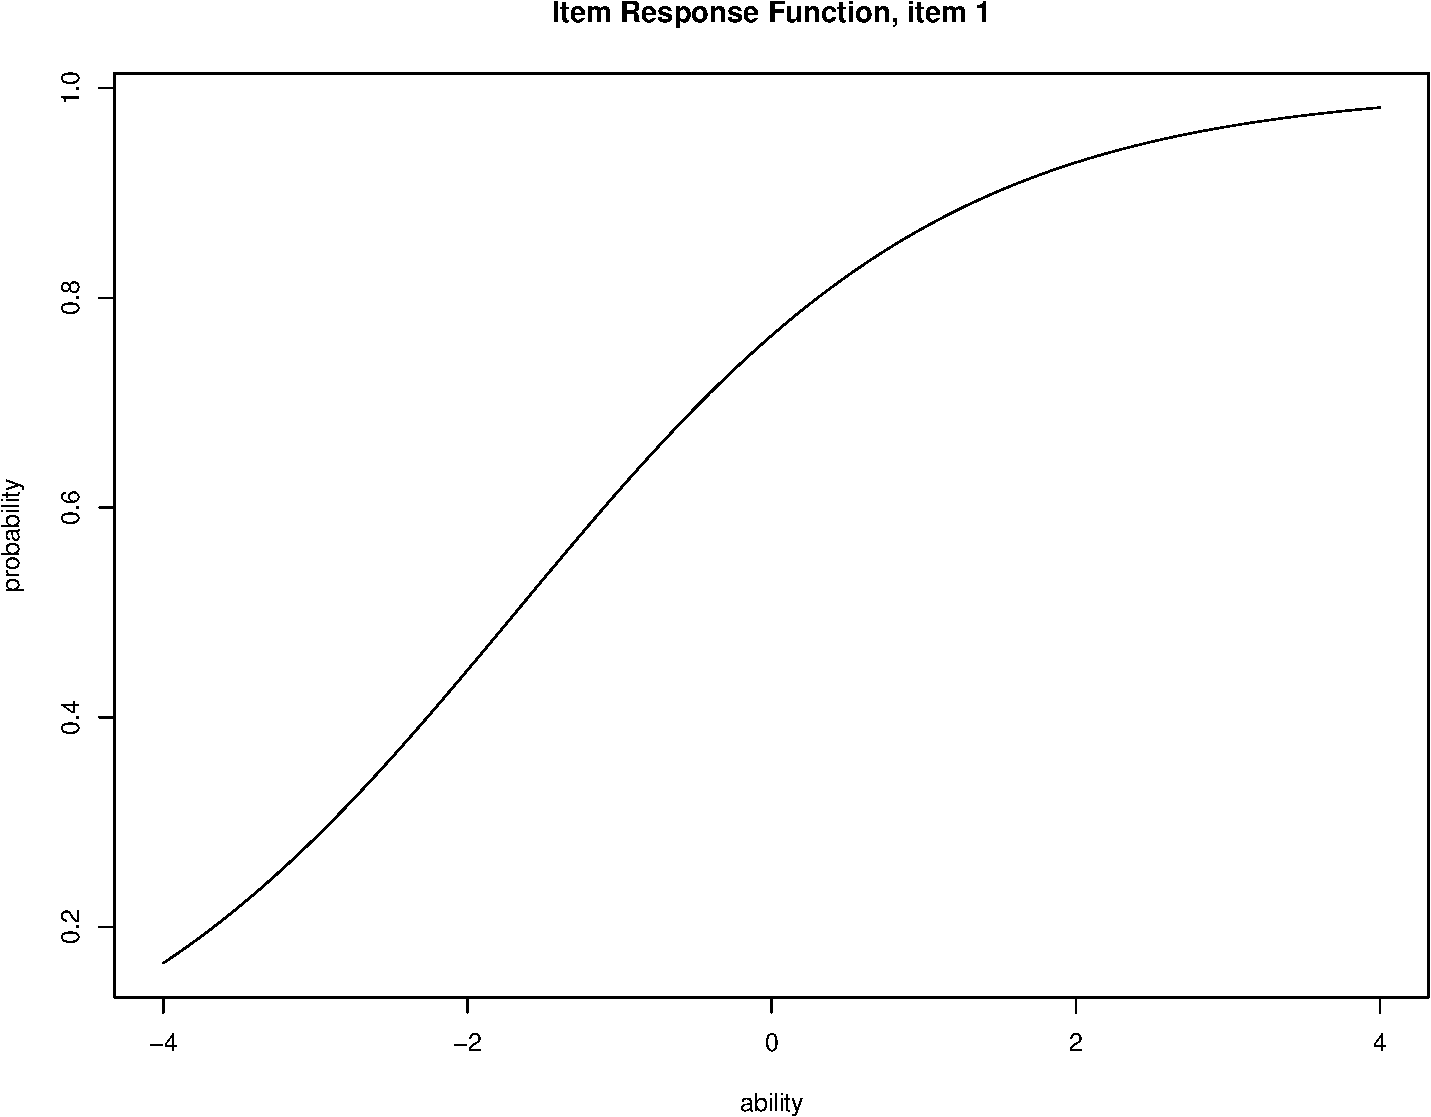
\includegraphics[keepaspectratio]{chap4_IRT_files/figure-pdf/unnamed-chunk-4-1.pdf}}

\begin{itemize}
\tightlist
\item
  項目反応関数(IRF)を表示してみましょう

  \begin{itemize}
  \tightlist
  \item
    複数の項目を一気に表示するには,\texttt{overlay}オプションを\texttt{TRUE}にするか,配置の行列指定(次頁)
  \end{itemize}
\end{itemize}

\begin{Shaded}
\begin{Highlighting}[]
\FunctionTok{plot}\NormalTok{(result, }\AttributeTok{items =} \DecValTok{1}\SpecialCharTok{:}\DecValTok{6}\NormalTok{, }\AttributeTok{type =} \StringTok{"IRF"}\NormalTok{, }\AttributeTok{overlay =} \ConstantTok{TRUE}\NormalTok{)}
\end{Highlighting}
\end{Shaded}

\pandocbounded{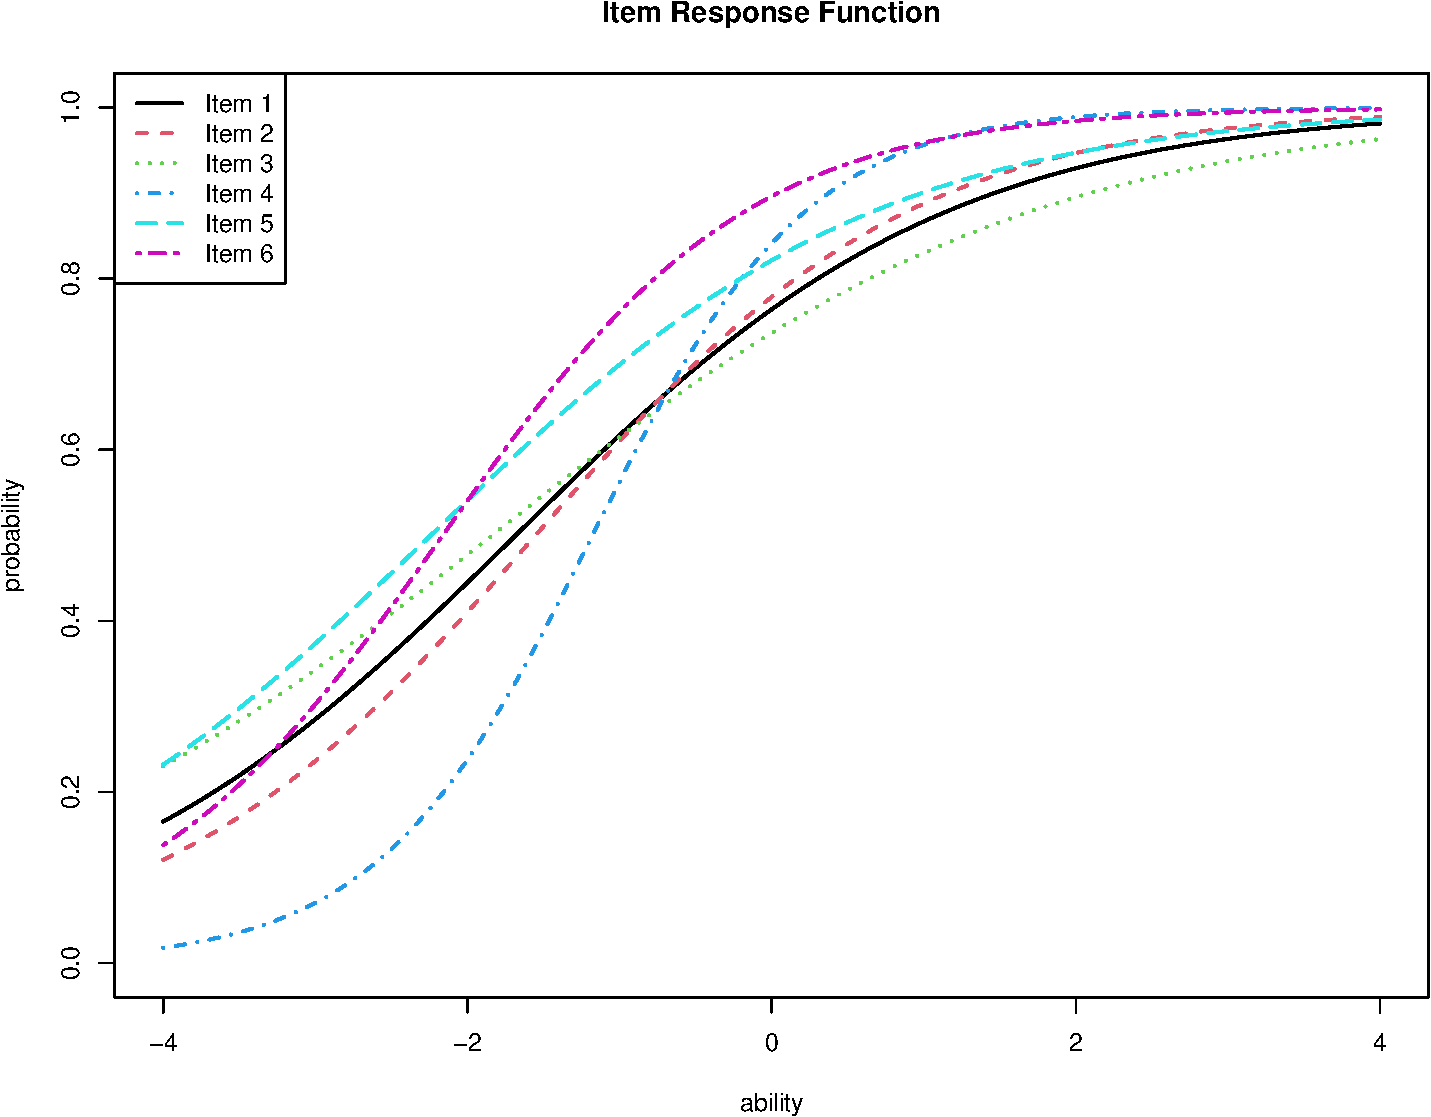
\includegraphics[keepaspectratio]{chap4_IRT_files/figure-pdf/unnamed-chunk-5-1.pdf}}

\begin{itemize}
\tightlist
\item
  項目反応関数(IRF)を表示してみましょう

  \begin{itemize}
  \tightlist
  \item
    複数の項目を一気に表示するには,\texttt{overlay}オプションを\texttt{TRUE}にするか,配置の行列指定

    \begin{itemize}
    \tightlist
    \item
      \texttt{nr}で行数,\texttt{nc}で列数を指定できます
    \end{itemize}
  \end{itemize}
\end{itemize}

\begin{Shaded}
\begin{Highlighting}[]
\FunctionTok{plot}\NormalTok{(result, }\AttributeTok{items =} \DecValTok{1}\SpecialCharTok{:}\DecValTok{6}\NormalTok{, }\AttributeTok{type =} \StringTok{"IRF"}\NormalTok{, }\AttributeTok{nr =} \DecValTok{3}\NormalTok{, }\AttributeTok{nc =} \DecValTok{2}\NormalTok{)}
\end{Highlighting}
\end{Shaded}

\pandocbounded{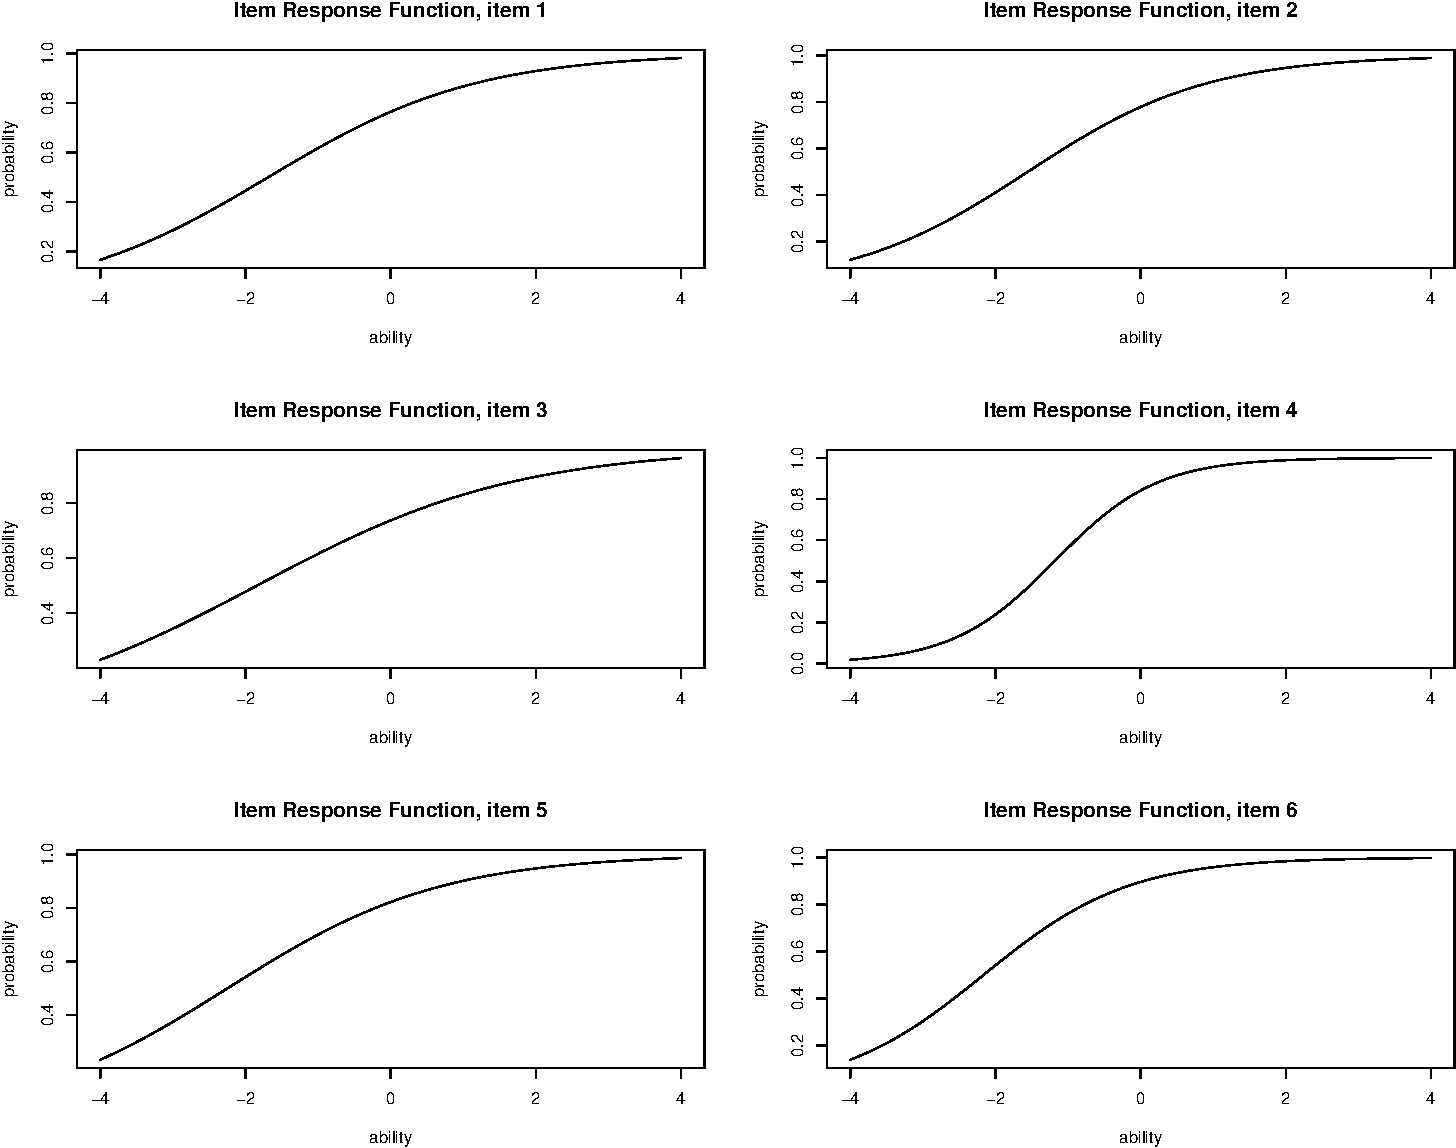
\includegraphics[keepaspectratio]{chap4_IRT_files/figure-pdf/unnamed-chunk-6-1.pdf}}

\begin{itemize}
\tightlist
\item
  テスト反応関数(TRF)を表示してみましょう

  \begin{itemize}
  \tightlist
  \item
    \texttt{type=IRF}として,\texttt{items\ =0}としても同様の出力を得ます
  \end{itemize}
\end{itemize}

\begin{Shaded}
\begin{Highlighting}[]
\FunctionTok{plot}\NormalTok{(result, }\AttributeTok{type =} \StringTok{"TRF"}\NormalTok{)}
\end{Highlighting}
\end{Shaded}

\pandocbounded{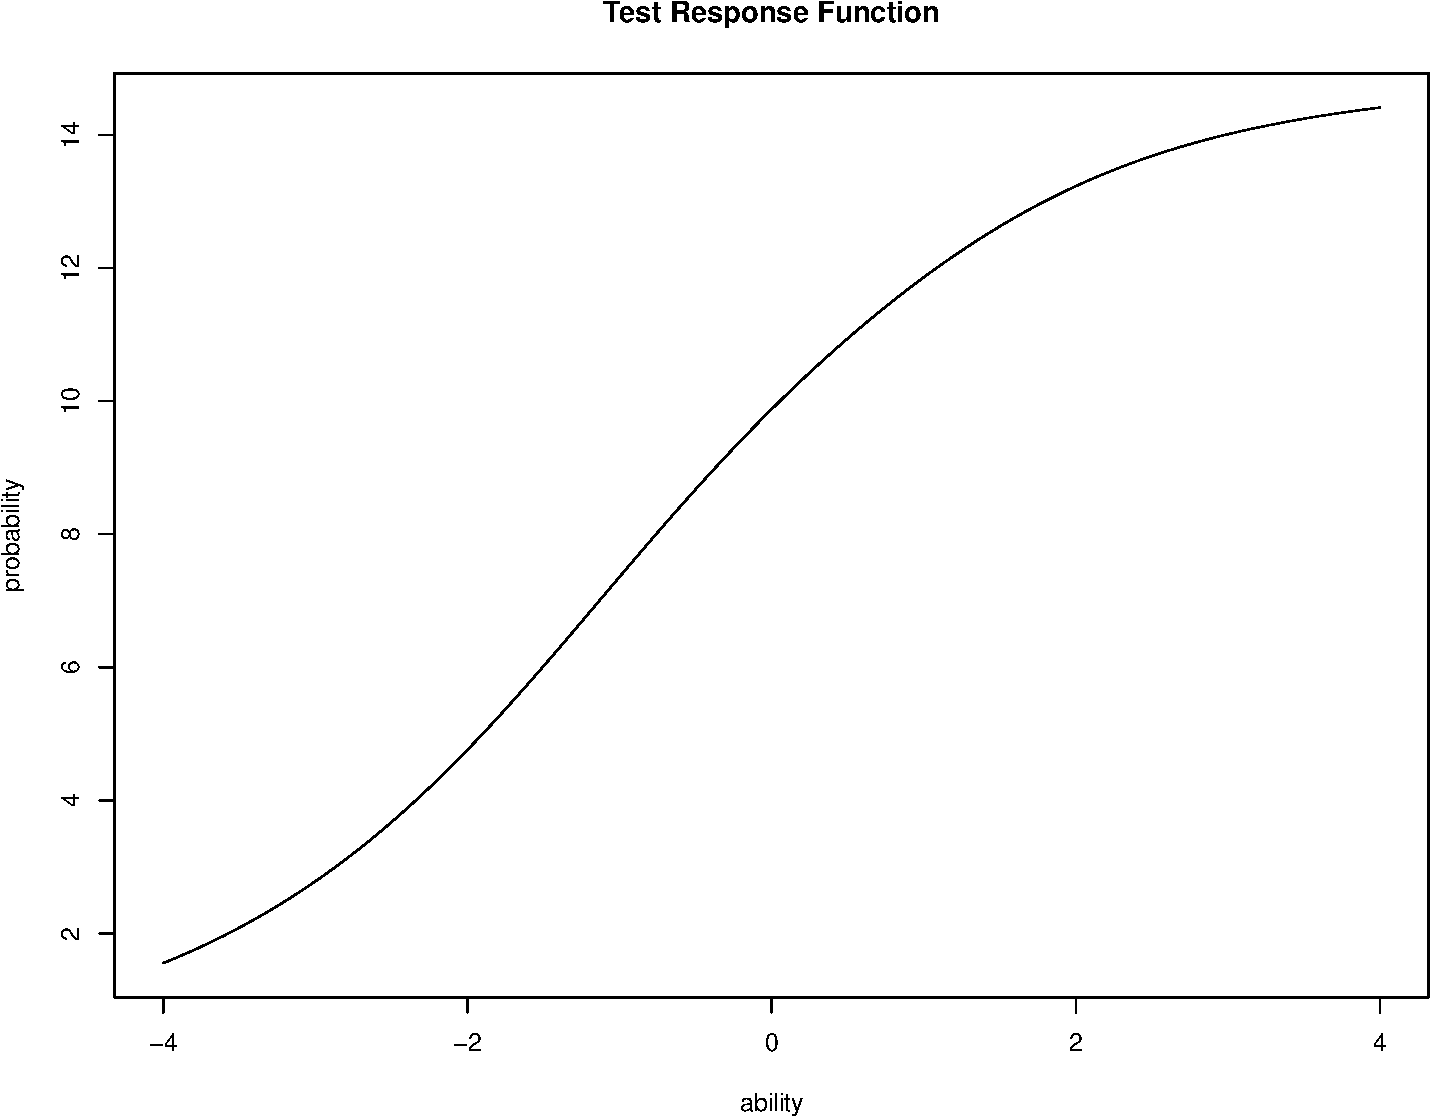
\includegraphics[keepaspectratio]{chap4_IRT_files/figure-pdf/unnamed-chunk-7-1.pdf}}

\begin{Shaded}
\begin{Highlighting}[]
\CommentTok{\# plot(result, type = "IRF", items = 0)}
\end{Highlighting}
\end{Shaded}

\begin{itemize}
\tightlist
\item
  項目情報関数(IIF)を表示してみましょう
\end{itemize}

\begin{Shaded}
\begin{Highlighting}[]
\FunctionTok{plot}\NormalTok{(result, }\AttributeTok{items =} \DecValTok{1}\SpecialCharTok{:}\DecValTok{15}\NormalTok{, }\AttributeTok{type =} \StringTok{"IIF"}\NormalTok{, }\AttributeTok{overlay =} \ConstantTok{TRUE}\NormalTok{)}
\end{Highlighting}
\end{Shaded}

\pandocbounded{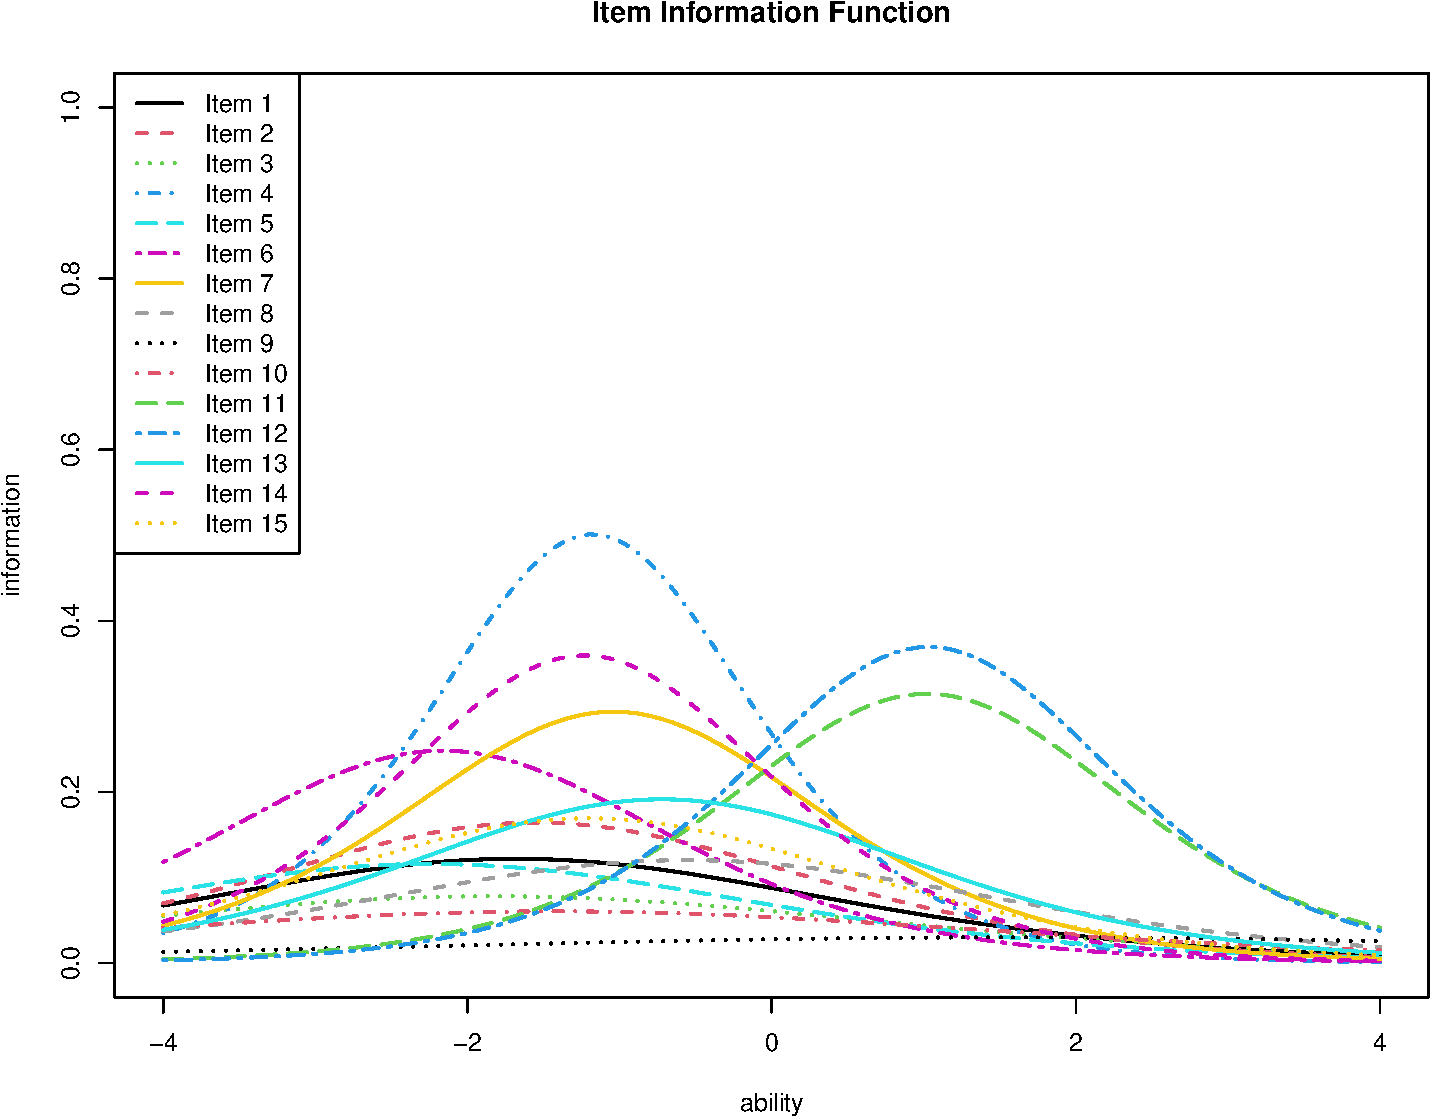
\includegraphics[keepaspectratio]{chap4_IRT_files/figure-pdf/unnamed-chunk-8-1.pdf}}

\begin{itemize}
\tightlist
\item
  テスト情報関数(TIF)を表示してみましょう
\end{itemize}

\begin{Shaded}
\begin{Highlighting}[]
\FunctionTok{plot}\NormalTok{(result, }\AttributeTok{type =} \StringTok{"TIF"}\NormalTok{)}
\end{Highlighting}
\end{Shaded}

\pandocbounded{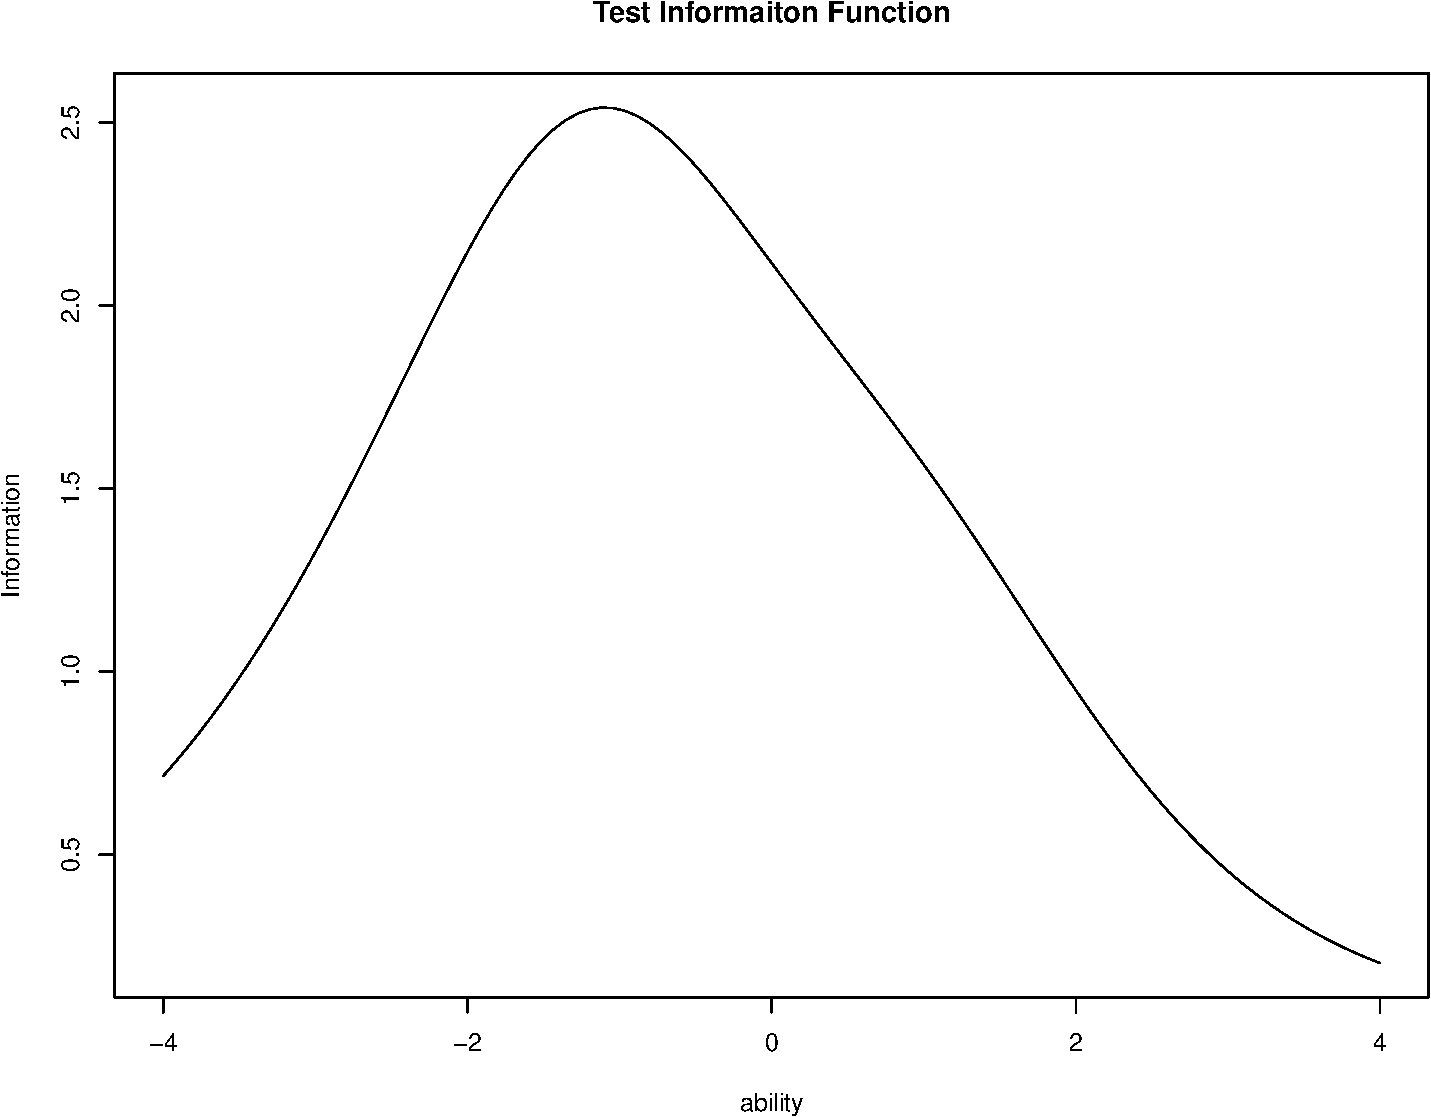
\includegraphics[keepaspectratio]{chap4_IRT_files/figure-pdf/unnamed-chunk-9-1.pdf}}

\begin{Shaded}
\begin{Highlighting}[]
\CommentTok{\# plot(result, items = 0, type = "IIF")}
\end{Highlighting}
\end{Shaded}

\subsection{受検者の情報も含まれています}\label{ux53d7ux691cux8005ux306eux60c5ux5831ux3082ux542bux307eux308cux3066ux3044ux307eux3059}

\begin{itemize}
\tightlist
\item
  EAP(Expectation A Posterior)推定値を出力します
\item
  PSD(Posterior Standard Deviation)も出力します
\end{itemize}

\begin{Shaded}
\begin{Highlighting}[]
\NormalTok{result}\SpecialCharTok{$}\NormalTok{ability }\SpecialCharTok{|\textgreater{}} \FunctionTok{head}\NormalTok{(}\DecValTok{20}\NormalTok{)}
\end{Highlighting}
\end{Shaded}

\begin{verbatim}
           ID         EAP       PSD
1  Student001 -0.66456782 0.5457047
2  Student002 -0.14853705 0.5626979
3  Student003  0.01362528 0.5699764
4  Student004  0.58775674 0.6012839
5  Student005 -0.97796882 0.5415527
6  Student006  0.85892500 0.6187224
7  Student007  0.05696142 0.5720482
8  Student008  0.04790637 0.5716114
9  Student009  1.23035677 0.6433918
10 Student010 -0.19705233 0.5606753
11 Student011 -0.34067166 0.5551509
12 Student012 -0.51385231 0.5495270
13 Student013  1.05114795 0.6316587
14 Student014  0.81625119 0.6158908
15 Student015 -1.35345901 0.5440715
16 Student016 -1.53285011 0.5476038
17 Student017  0.62954564 0.6038740
18 Student018 -0.96955171 0.5415908
19 Student019  0.73791232 0.6107655
20 Student020 -0.80866493 0.5431159
\end{verbatim}

\subsection{Q3行列}\label{q3ux884cux5217}

\begin{itemize}
\tightlist
\item
  局所独立の仮定が満たされているかどうかを判断する指標として,Q3行列があります

  \begin{itemize}
  \tightlist
  \item
    項目特性同士の相関行列です
  \item
    この値が高すぎると局所独立の仮定が満たされていない可能性があります
  \end{itemize}
\end{itemize}

\begin{Shaded}
\begin{Highlighting}[]
\NormalTok{result}\SpecialCharTok{$}\NormalTok{Q3mat}
\end{Highlighting}
\end{Shaded}

\begin{verbatim}
        Item01  Item02   Item03   Item04   Item05   Item06   Item07  Item08
Item01  1.0000 -0.0535 -0.08856 -0.13197  0.05521  0.01128 -0.09982  0.0139
Item02 -0.0535  1.0000  0.00440 -0.02750 -0.02981 -0.03641 -0.10196 -0.0638
Item03 -0.0886  0.0044  1.00000  0.00363  0.00902  0.00334  0.01898 -0.0465
Item04 -0.1320 -0.0275  0.00363  1.00000 -0.08089 -0.12016 -0.03221 -0.0855
Item05  0.0552 -0.0298  0.00902 -0.08089  1.00000 -0.06635 -0.04430 -0.0596
Item06  0.0113 -0.0364  0.00334 -0.12016 -0.06635  1.00000 -0.02694  0.0255
Item07 -0.0998 -0.1020  0.01898 -0.03221 -0.04430 -0.02694  1.00000 -0.0245
Item08  0.0139 -0.0638 -0.04653 -0.08547 -0.05961  0.02546 -0.02450  1.0000
Item09  0.0191 -0.0541 -0.03816 -0.05523 -0.08799 -0.07573 -0.01889 -0.0744
Item10 -0.0392 -0.0409 -0.02099 -0.09241 -0.01727 -0.02101  0.00508 -0.0625
Item11 -0.0281 -0.0171 -0.07191 -0.07304 -0.05427 -0.10232 -0.06882  0.0049
Item12 -0.0683 -0.0562 -0.07754 -0.01098 -0.06810 -0.09014 -0.07219 -0.0672
Item13 -0.0342 -0.0820 -0.01490 -0.07015  0.02738 -0.08209 -0.10070 -0.0297
Item14 -0.0209 -0.0496 -0.11632 -0.16292 -0.04666 -0.02432 -0.15965 -0.1019
Item15 -0.0343 -0.0436 -0.07199 -0.03444 -0.05169  0.03602 -0.05857 -0.0781
         Item09   Item10   Item11  Item12   Item13   Item14  Item15
Item01  0.01906 -0.03915 -0.02813 -0.0683 -0.03423 -0.02090 -0.0343
Item02 -0.05412 -0.04094 -0.01708 -0.0562 -0.08200 -0.04963 -0.0436
Item03 -0.03816 -0.02099 -0.07191 -0.0775 -0.01490 -0.11632 -0.0720
Item04 -0.05523 -0.09241 -0.07304 -0.0110 -0.07015 -0.16292 -0.0344
Item05 -0.08799 -0.01727 -0.05427 -0.0681  0.02738 -0.04666 -0.0517
Item06 -0.07573 -0.02101 -0.10232 -0.0901 -0.08209 -0.02432  0.0360
Item07 -0.01889  0.00508 -0.06882 -0.0722 -0.10070 -0.15965 -0.0586
Item08 -0.07436 -0.06251  0.00490 -0.0672 -0.02972 -0.10189 -0.0781
Item09  1.00000 -0.10174 -0.05357  0.0772 -0.00977  0.01932 -0.0708
Item10 -0.10174  1.00000 -0.02597 -0.0902  0.01259  0.02296 -0.0529
Item11 -0.05357 -0.02597  1.00000 -0.0630 -0.15170  0.00762 -0.0948
Item12  0.07724 -0.09020 -0.06302  1.0000 -0.09172 -0.05197 -0.0887
Item13 -0.00977  0.01259 -0.15170 -0.0917  1.00000 -0.03881  0.0113
Item14  0.01932  0.02296  0.00762 -0.0520 -0.03881  1.00000 -0.0680
Item15 -0.07085 -0.05290 -0.09481 -0.0887  0.01128 -0.06801  1.0000
\end{verbatim}

\section{多値への展開}\label{ux591aux5024ux3078ux306eux5c55ux958b-1}

\subsection{段階反応モデル}\label{ux6bb5ux968eux53cdux5fdcux30e2ux30c7ux30eb}

\begin{itemize}
\tightlist
\item
  段階反応モデルは順序的な反応段階を仮定したモデルです

  \begin{itemize}
  \tightlist
  \item
    K段階カテゴリのデータがあったとして,k以上のカテゴリに反応する確率を2PLモデルのように推定します。
  \end{itemize}
\item
  サンプルデータ\texttt{J5S1000}で様子を見てみましょう
\end{itemize}

\begin{Shaded}
\begin{Highlighting}[]
\NormalTok{dat }\OtherTok{\textless{}{-}}\NormalTok{ J5S1000}
\FunctionTok{TestStatistics}\NormalTok{(dat)}
\end{Highlighting}
\end{Shaded}

\begin{verbatim}
Test Statistics
                   value
SampleSize 1000.00000000
TestLength    5.00000000
Median       12.00000000
Max          18.00000000
Min           4.00000000
Range        14.00000000
Mean         11.45700000
SD            2.92107578
Skewness     -0.08836075
Kurtosis     -0.55776379
Alpha         0.59462241
\end{verbatim}

\begin{itemize}
\tightlist
\item
  \texttt{exametrika}の性能(精度+実行速度)はそこまで高くないので、\texttt{ltm}パッケージや\texttt{mirt}パッケージなども参考にしてください。
\item
\end{itemize}

\begin{Shaded}
\begin{Highlighting}[]
\NormalTok{result.GRM }\OtherTok{\textless{}{-}} \FunctionTok{GRM}\NormalTok{(dat)}
\end{Highlighting}
\end{Shaded}

\begin{verbatim}
initial  value 6497.015125 
iter  10 value 6046.073326
iter  20 value 6013.787923
iter  30 value 6008.297277
final  value 6008.297277 
converged
\end{verbatim}

\begin{Shaded}
\begin{Highlighting}[]
\NormalTok{result.GRM}
\end{Highlighting}
\end{Shaded}

\begin{verbatim}
Item Parameter
   Descriminate Threshold1 Threshold2 Threshold3
V1        0.927      -1.54     0.0512       1.53
V2        1.234      -1.21     1.3936         NA
V3        0.917      -1.60    -0.0757       1.27
V4        1.479      -1.44     1.3166         NA
V5        0.947      -1.37     0.0286       1.54

Item Fit Indices
     NFI   RFI   IFI   TLI   CFI RMSEA     AIC    CAIC     BIC
V1 0.248 0.265 0.271 0.288 0.272 0.090 324.819  99.017  99.063
V2 0.219 0.244 0.236 0.263 0.238 0.098 263.864 111.692 111.723
V3 0.253 0.269 0.276 0.293 0.277 0.089 321.824  96.021  96.067
V4 0.000 0.000 0.000 0.000 0.000 0.132 512.023 359.852 359.883
V5 0.255 0.272 0.278 0.295 0.279 0.090 327.598 101.795 101.841

Model Fit Indices
         value
NFI      0.165
RFI      0.186
IFI      0.179
TLI      0.201
CFI      0.180
RMSEA    0.099
AIC   1750.128
CAIC   768.377
BIC    768.577
\end{verbatim}

\subsection{可視化しましょう}\label{ux53efux8996ux5316ux3057ux307eux3057ux3087ux3046-1}

\begin{itemize}
\tightlist
\item
  IRTモデルと同じように,IRFを出力することができます。
\end{itemize}

\begin{Shaded}
\begin{Highlighting}[]
\FunctionTok{plot}\NormalTok{(result.GRM, }\AttributeTok{type =} \StringTok{"IRF"}\NormalTok{, }\AttributeTok{items =} \DecValTok{2}\NormalTok{)}
\end{Highlighting}
\end{Shaded}

\pandocbounded{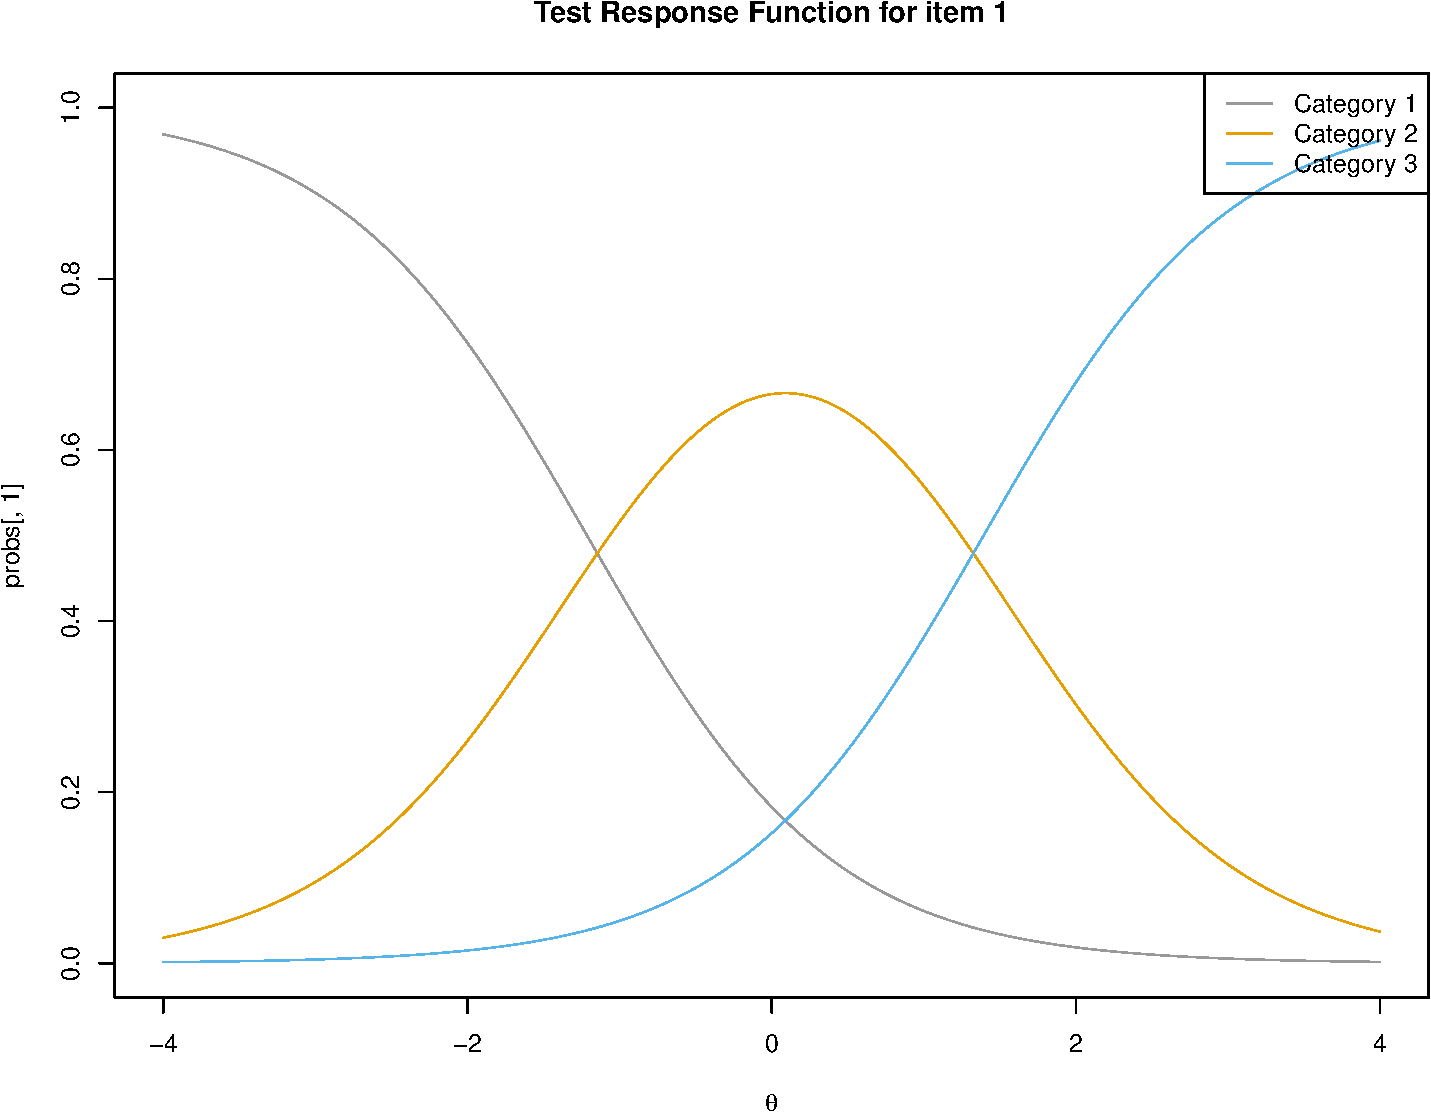
\includegraphics[keepaspectratio]{chap4_IRT_files/figure-pdf/unnamed-chunk-13-1.pdf}}

\begin{Shaded}
\begin{Highlighting}[]
\FunctionTok{plot}\NormalTok{(result.GRM, }\AttributeTok{type =} \StringTok{"IRF"}\NormalTok{, }\AttributeTok{items =} \FunctionTok{c}\NormalTok{(}\DecValTok{1}\NormalTok{, }\DecValTok{3}\NormalTok{, }\DecValTok{4}\NormalTok{, }\DecValTok{5}\NormalTok{))}
\end{Highlighting}
\end{Shaded}

\pandocbounded{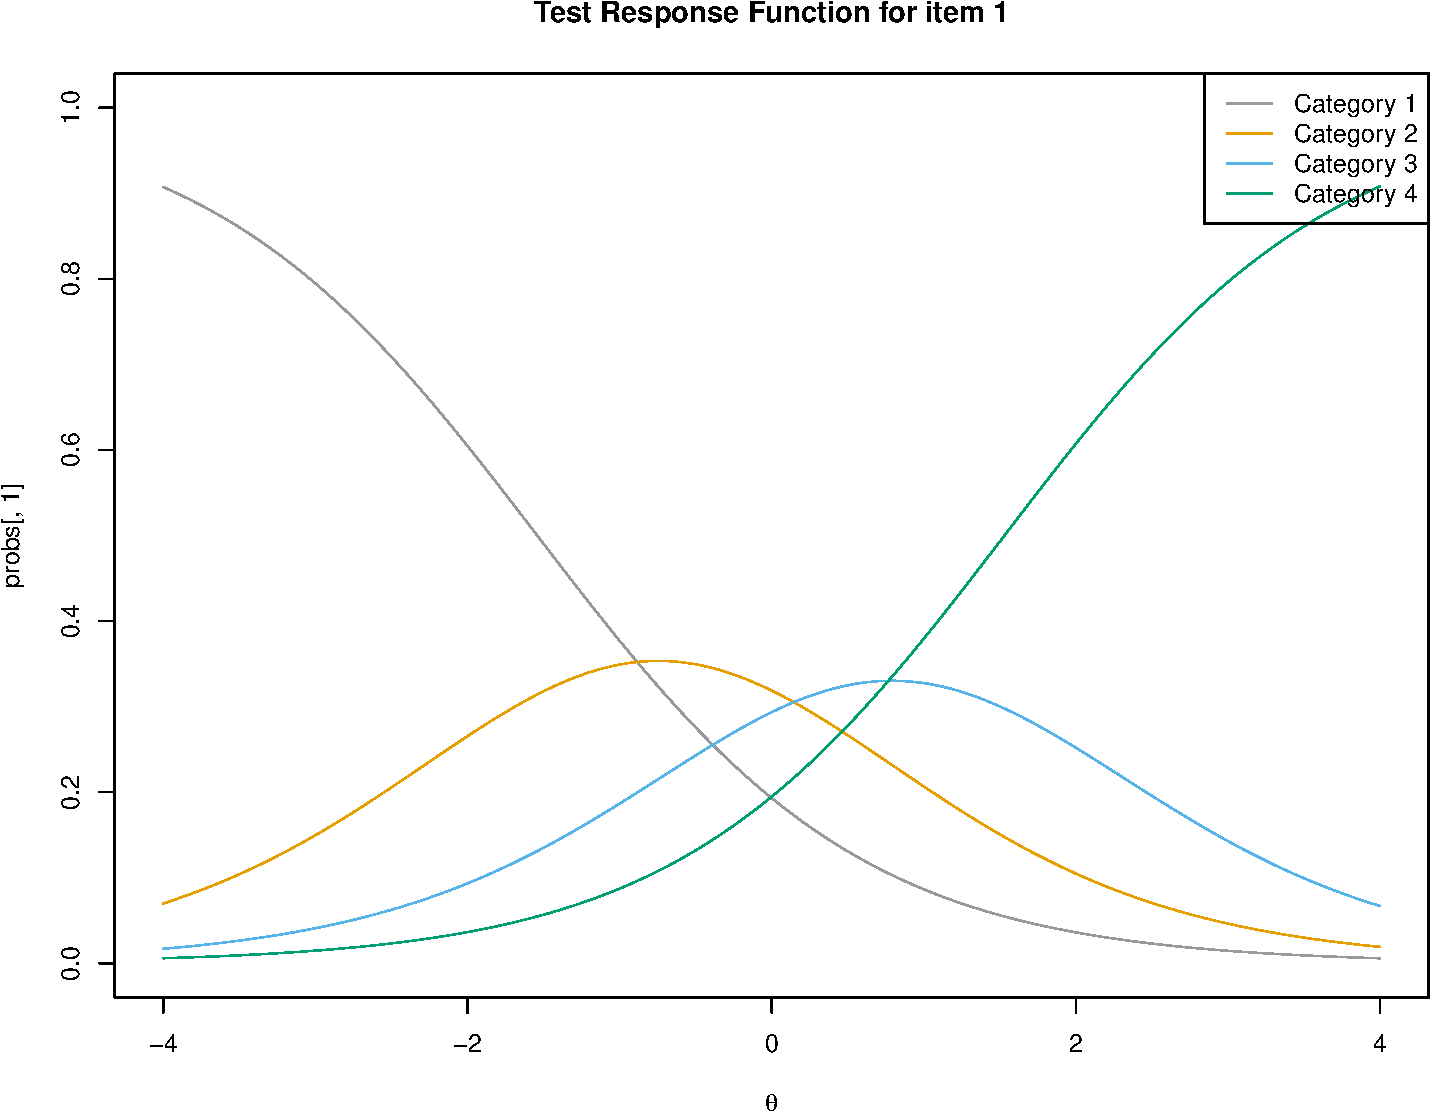
\includegraphics[keepaspectratio]{chap4_IRT_files/figure-pdf/unnamed-chunk-13-2.pdf}}

\pandocbounded{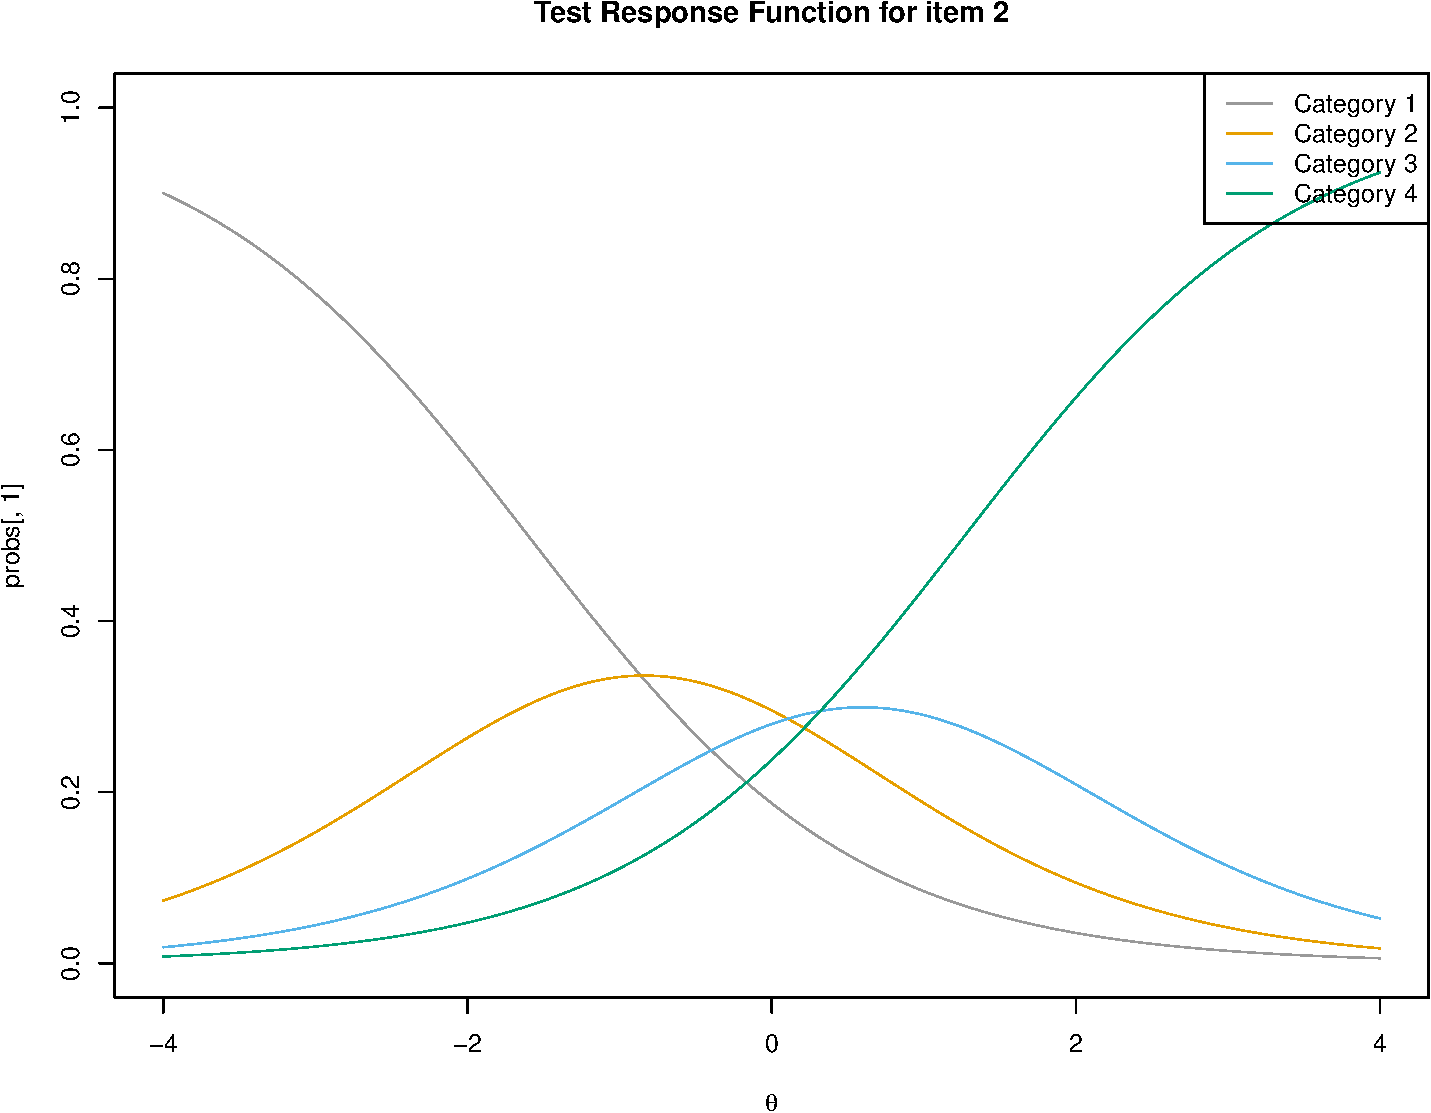
\includegraphics[keepaspectratio]{chap4_IRT_files/figure-pdf/unnamed-chunk-13-3.pdf}}

\pandocbounded{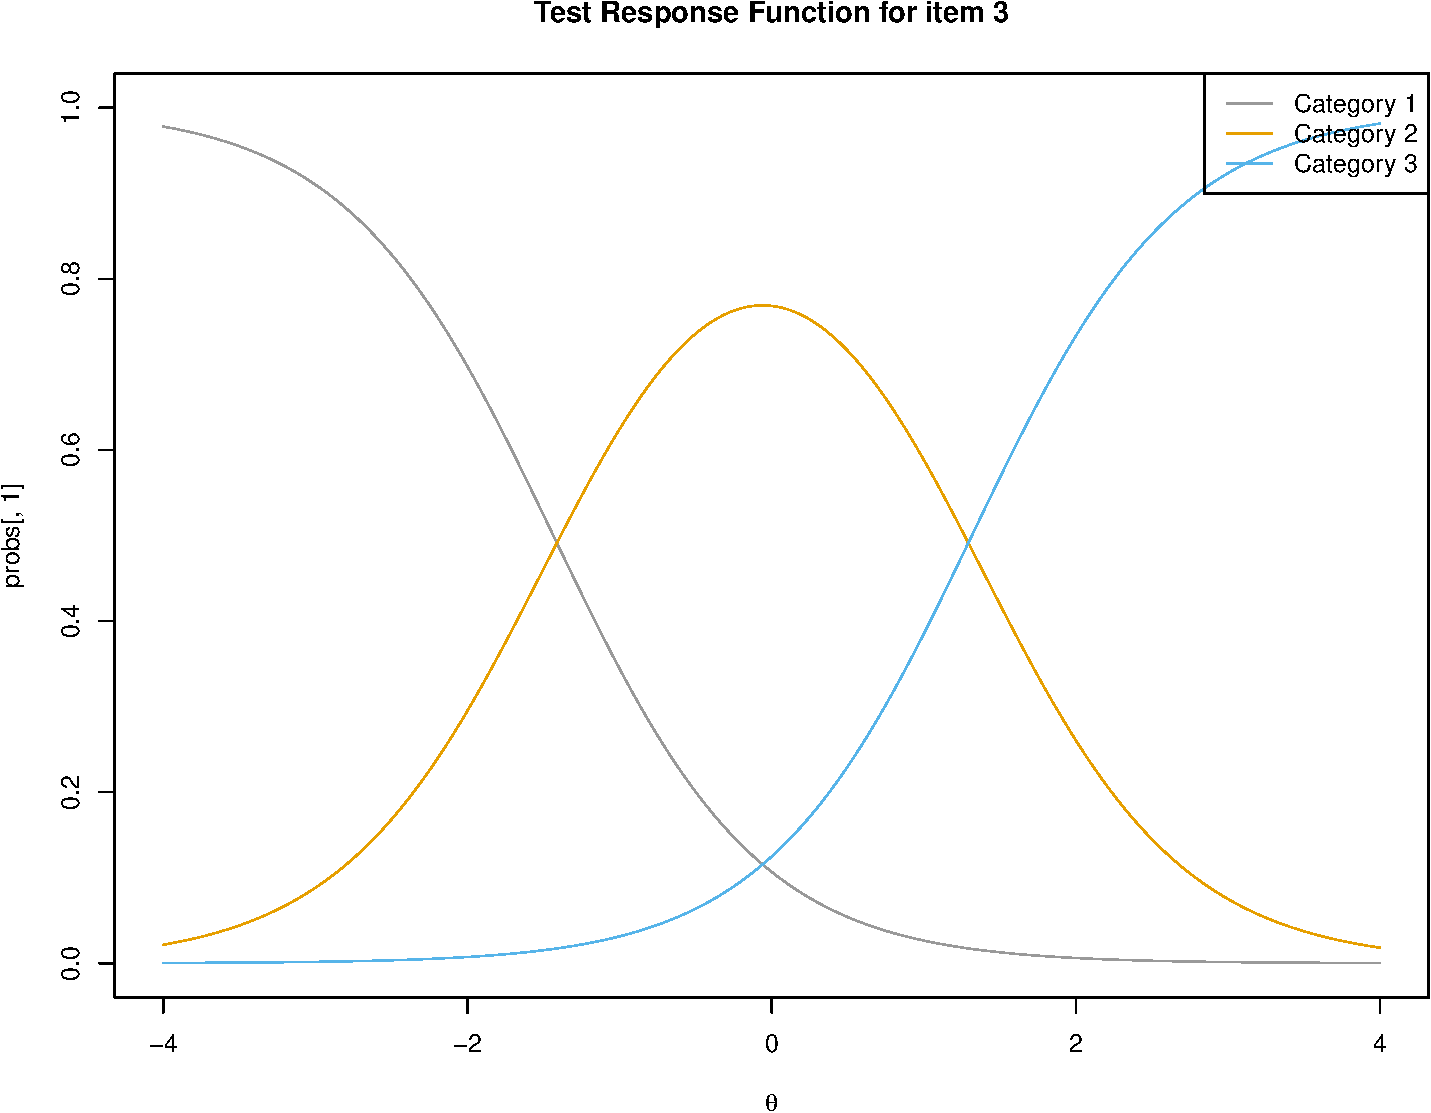
\includegraphics[keepaspectratio]{chap4_IRT_files/figure-pdf/unnamed-chunk-13-4.pdf}}

\pandocbounded{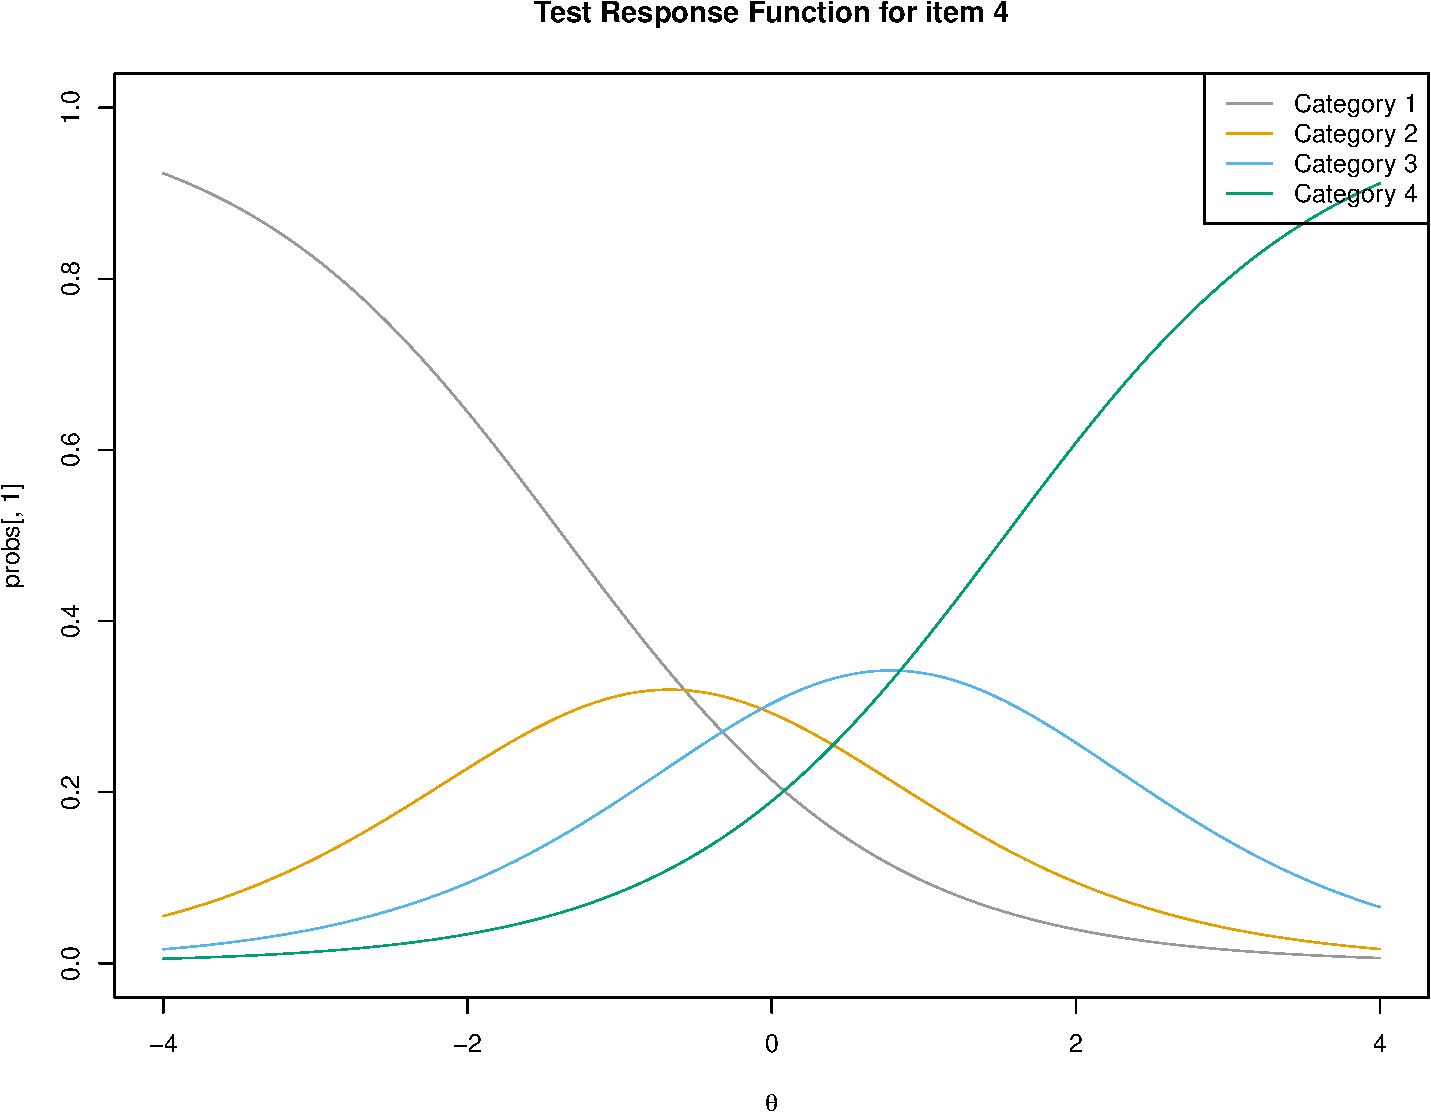
\includegraphics[keepaspectratio]{chap4_IRT_files/figure-pdf/unnamed-chunk-13-5.pdf}}

\begin{itemize}
\tightlist
\item
  IRTモデルと同じように,IIFを出力することができます。
\end{itemize}

\begin{Shaded}
\begin{Highlighting}[]
\FunctionTok{plot}\NormalTok{(result.GRM, }\AttributeTok{type =} \StringTok{"IIF"}\NormalTok{, }\AttributeTok{nr =} \DecValTok{2}\NormalTok{, }\AttributeTok{nc =} \DecValTok{2}\NormalTok{)}
\end{Highlighting}
\end{Shaded}

\pandocbounded{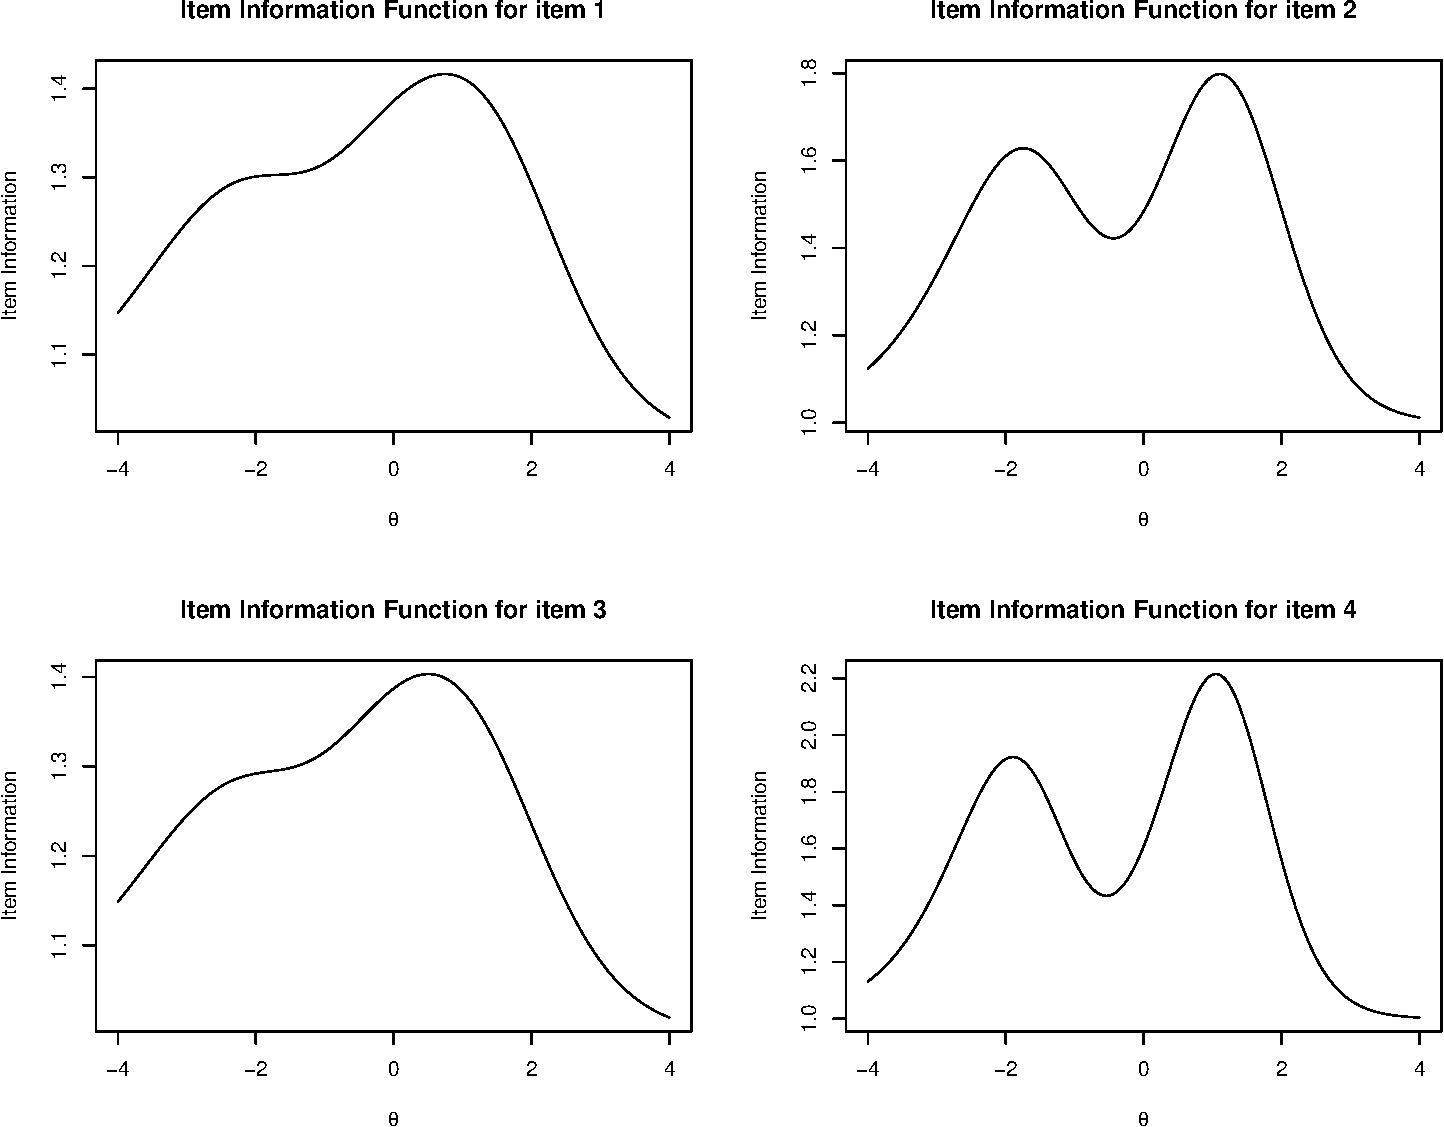
\includegraphics[keepaspectratio]{chap4_IRT_files/figure-pdf/unnamed-chunk-14-1.pdf}}

\pandocbounded{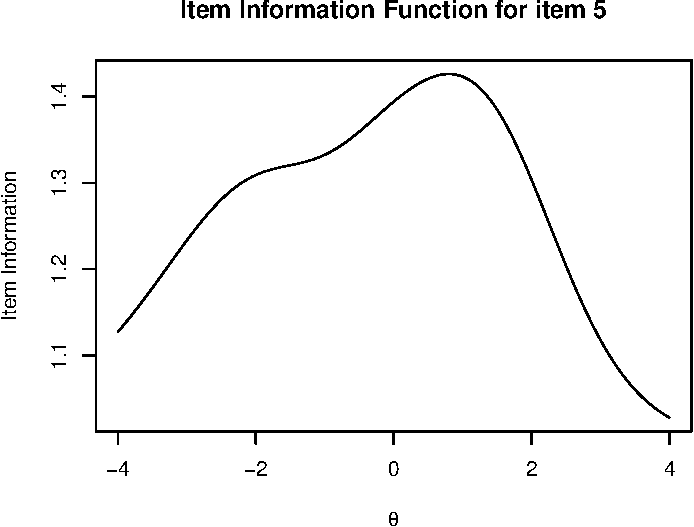
\includegraphics[keepaspectratio]{chap4_IRT_files/figure-pdf/unnamed-chunk-14-2.pdf}}

\begin{itemize}
\tightlist
\item
  IRTモデルと同じように,TIFを出力することができます。
\end{itemize}

\begin{Shaded}
\begin{Highlighting}[]
\FunctionTok{plot}\NormalTok{(result.GRM, }\AttributeTok{type =} \StringTok{"TIF"}\NormalTok{)}
\end{Highlighting}
\end{Shaded}

\pandocbounded{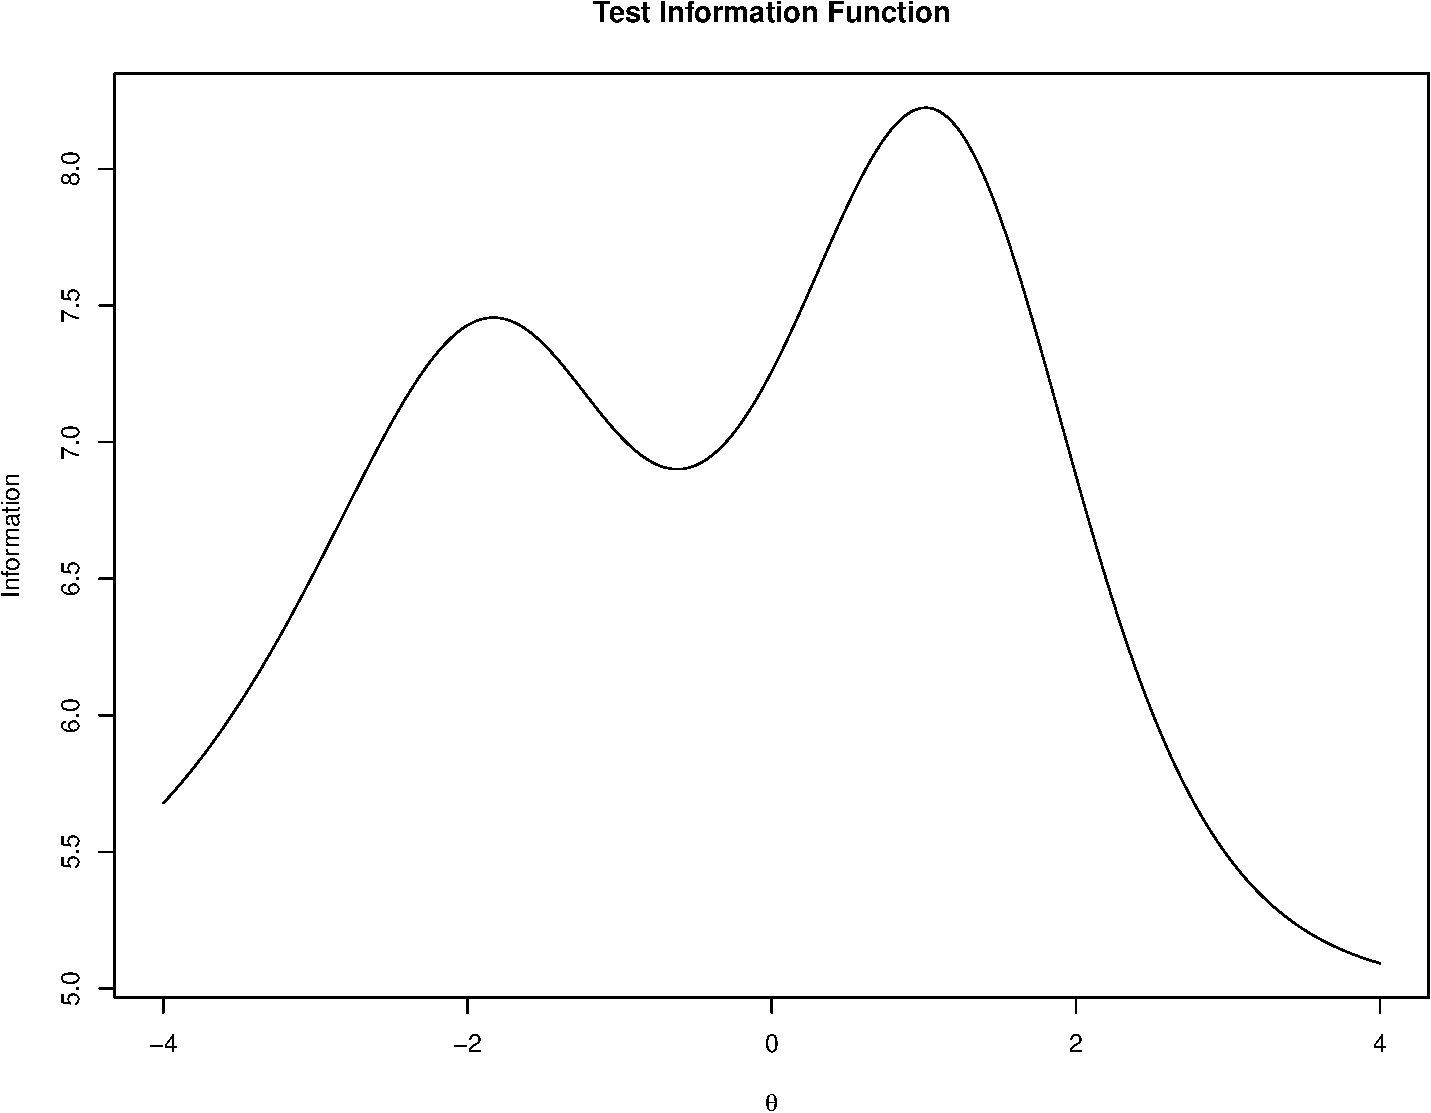
\includegraphics[keepaspectratio]{chap4_IRT_files/figure-pdf/unnamed-chunk-15-1.pdf}}

\section{コラム:GRMと他のモデル}\label{ux30b3ux30e9ux30e0grmux3068ux4ed6ux306eux30e2ux30c7ux30eb}

\begin{itemize}
\tightlist
\item
  段階反応モデルは正規分布する連続的潜在変数\(\theta\)を仮定して,数値が高くなるとより上位のカテゴリに反応しやすくなるモデルです。

  \begin{itemize}
  \tightlist
  \item
    社会的態度を測定するリッカート法のIRT版とも言えます
  \item
    反応カテゴリに順序性を仮定した因子分析と数学的に等価です
  \item
    カテゴリ反応で多因子モデルの場合,\texttt{mirt}パッケージ(Multidimensional
    IRT)や\texttt{lavaan}パッケージ(LAtent VAriable
    ANalysis)で推定しましょう
  \end{itemize}
\item
  IRFを見ることで,項目カテゴリが反応段階を弁別できているかチェックできます
\end{itemize}

\section{コラム:態度測定論}\label{ux30b3ux30e9ux30e0ux614bux5ea6ux6e2cux5b9aux8ad6}

\begin{itemize}
\tightlist
\item
  \textbf{社会的態度}は社会心理学の分野で考えられてきた連続的潜在変数です

  \begin{itemize}
  \tightlist
  \item
    サーストンの考えた測定方法(等現間隔法)をつかって測定する,一次元モデルです
  \item
    リッカートの方法はサーストン法の簡易版として出てきた態度モデルです
  \end{itemize}
\item
  昨今は,「心の測定」,「心理学的連続体」,「心理尺度の妥当性」が問題になっています
\item
  心理尺度(リッカート法)は一朝一夕に作れるものではありません
\item
  心理尺度は領域,方法,標準化など使用法によく注意して利用しましょう
\end{itemize}

\bookmarksetup{startatroot}

\chapter{Rをつかった潜在クラス/ランク分析の実習}\label{rux3092ux3064ux304bux3063ux305fux6f5cux5728ux30afux30e9ux30b9ux30e9ux30f3ux30afux5206ux6790ux306eux5b9fux7fd2}

\section{準備しましょう}\label{ux6e96ux5099ux3057ux307eux3057ux3087ux3046-2}

\subsection{サンプルデータを用います}\label{ux30b5ux30f3ux30d7ux30ebux30c7ux30fcux30bfux3092ux7528ux3044ux307eux3059-1}

\begin{itemize}
\tightlist
\item
  RStudioでプロジェクトを開いているか確認してくださいね
\item
  \texttt{exametrika}が持っている\texttt{J15S500}を例にします
\end{itemize}

\begin{Shaded}
\begin{Highlighting}[]
\FunctionTok{library}\NormalTok{(exametrika)}
\end{Highlighting}
\end{Shaded}

\begin{verbatim}
Loading required package: mvtnorm
\end{verbatim}

\begin{verbatim}
Loading required package: igraph
\end{verbatim}

\begin{verbatim}

Attaching package: 'igraph'
\end{verbatim}

\begin{verbatim}
The following objects are masked from 'package:stats':

    decompose, spectrum
\end{verbatim}

\begin{verbatim}
The following object is masked from 'package:base':

    union
\end{verbatim}

\begin{Shaded}
\begin{Highlighting}[]
\NormalTok{dat }\OtherTok{\textless{}{-}}\NormalTok{ J15S500}
\FunctionTok{TestStatistics}\NormalTok{(dat)}
\end{Highlighting}
\end{Shaded}

\begin{verbatim}
Test Statistics
                  value
TestLength   15.0000000
SampleSize  500.0000000
Mean          9.6640000
SEofMean      0.1190738
Variance      7.0892826
SD            2.6625707
Skewness     -0.4116220
Kurtosis     -0.4471624
Min           2.0000000
Max          15.0000000
Range        13.0000000
Q1.25%        8.0000000
Median.50%   10.0000000
Q3.75%       12.0000000
IQR.75%       4.0000000
Stanine.4%    5.0000000
Stanine.11%   6.0000000
Stanine.23%   7.0000000
Stanine.40%   9.0000000
Stanine.60%  11.0000000
Stanine.77%  12.0000000
Stanine.89%  13.0000000
Stanine.96%  14.0000000
\end{verbatim}

\subsection{潜在クラス分析をやってみよう}\label{ux6f5cux5728ux30afux30e9ux30b9ux5206ux6790ux3092ux3084ux3063ux3066ux307fux3088ux3046}

\begin{itemize}
\tightlist
\item
  潜在クラス(Latent Class
  Analysis)分析は,受検者を潜在的なグループに分類するモデルです
\item
  \texttt{LCA}関数で実行できます
\end{itemize}

\begin{Shaded}
\begin{Highlighting}[]
\NormalTok{result.LCA }\OtherTok{\textless{}{-}} \FunctionTok{LCA}\NormalTok{(dat, }\AttributeTok{ncls =} \DecValTok{6}\NormalTok{)}
\NormalTok{result.LCA}
\end{Highlighting}
\end{Shaded}

\begin{verbatim}

Item Reference Profile
         IRP1   IRP2    IRP3  IRP4   IRP5  IRP6
Item01 0.4370 0.7608 0.73618 0.789 0.8459 0.883
Item02 0.5916 0.4784 0.75372 0.990 0.8738 0.805
Item03 0.7695 0.4027 0.89807 0.673 0.7384 0.855
Item04 0.5757 0.3974 0.87205 0.883 0.8866 1.000
Item05 0.6023 0.7820 0.94283 0.797 0.7931 0.883
Item06 0.6508 0.7042 0.92835 0.988 1.0000 0.881
Item07 0.5395 0.3102 0.82178 0.757 0.9169 0.910
Item08 0.3767 0.3255 0.60377 0.670 0.8828 0.635
Item09 0.2945 0.3467 0.16135 0.636 0.0107 0.739
Item10 0.5200 0.5570 0.79602 0.552 0.7070 0.819
Item11 0.1053 0.0472 0.00488 0.208 0.6864 0.656
Item12 0.0729 0.0776 0.16864 0.244 0.3015 0.764
Item13 0.2142 0.4370 0.95899 0.649 0.6426 0.842
Item14 0.2379 0.7530 0.76640 0.874 0.9085 1.000
Item15 0.3935 0.5389 0.86050 0.717 0.8220 0.863

Test Profile
                              Class 1 Class 2 Class 3 Class 4 Class 5 Class 6
Test Reference Profile          6.381   6.919  10.274  10.428  11.016  12.535
Latent Class Ditribution       76.000  74.000 105.000  82.000  91.000  72.000
Class Membership Distribution  77.345  80.034  88.778  85.807  84.592  83.444

Item Fit Indices
       model_log_like bench_log_like null_log_like model_Chi_sq null_Chi_sq
Item01       -258.896       -240.190      -283.343       37.414      86.307
Item02       -235.421       -235.436      -278.949       -0.032      87.025
Item03       -262.373       -260.906      -293.598        2.934      65.383
Item04       -201.256       -192.072      -265.962       18.369     147.780
Item05       -230.005       -206.537      -247.403       46.935      81.732
Item06       -157.551       -153.940      -198.817        7.223      89.755
Item07       -241.548       -228.379      -298.345       26.338     139.933
Item08       -301.042       -293.225      -338.789       15.634      91.127
Item09       -246.942       -300.492      -327.842     -107.100      54.700
Item10       -303.019       -288.198      -319.850       29.641      63.303
Item11       -194.120       -224.085      -299.265      -59.931     150.360
Item12       -227.324       -214.797      -293.598       25.054     157.603
Item13       -257.389       -262.031      -328.396       -9.282     132.730
Item14       -193.802       -204.953      -273.212      -22.302     136.519
Item15       -267.063       -254.764      -302.847       24.598      96.166
       model_df null_df   NFI   RFI   IFI   TLI   CFI RMSEA      AIC     CAIC
Item01        8      13 0.567 0.296 0.624 0.348 0.599 0.086   21.414  -12.319
Item02        8      13 1.000 1.000 1.000 1.000 1.000 0.000  -16.032  -49.765
Item03        8      13 0.955 0.927 1.000 1.000 1.000 0.000  -13.066  -46.799
Item04        8      13 0.876 0.798 0.926 0.875 0.923 0.051    2.369  -31.364
Item05        8      13 0.426 0.067 0.472 0.079 0.434 0.099   30.935   -2.798
Item06        8      13 0.920 0.869 1.000 1.000 1.000 0.000   -8.777  -42.510
Item07        8      13 0.812 0.694 0.861 0.765 0.856 0.068   10.338  -23.395
Item08        8      13 0.828 0.721 0.908 0.841 0.902 0.044   -0.366  -34.099
Item09        8      13 1.000 1.000 1.000 1.000 1.000 0.000 -123.100 -156.833
Item10        8      13 0.532 0.239 0.609 0.301 0.570 0.074   13.641  -20.092
Item11        8      13 1.000 1.000 1.000 1.000 1.000 0.000  -75.931 -109.664
Item12        8      13 0.841 0.742 0.886 0.808 0.882 0.065    9.054  -24.679
Item13        8      13 1.000 1.000 1.000 1.000 1.000 0.000  -25.282  -59.015
Item14        8      13 1.000 1.000 1.000 1.000 1.000 0.000  -38.302  -72.035
Item15        8      13 0.744 0.584 0.812 0.676 0.800 0.064    8.598  -25.135
            BIC
Item01  -12.303
Item02  -49.749
Item03  -46.783
Item04  -31.348
Item05   -2.782
Item06  -42.494
Item07  -23.379
Item08  -34.083
Item09 -156.817
Item10  -20.076
Item11 -109.648
Item12  -24.663
Item13  -58.999
Item14  -72.019
Item15  -25.119

Model Fit Indices
Number of Latent class: 6
Number of EM cycle: 75 
                   value
model_log_like -3577.752
bench_log_like -3560.005
null_log_like  -4350.217
model_Chi_sq      35.494
null_Chi_sq     1580.424
model_df         120.000
null_df          195.000
NFI                0.978
RFI                0.964
IFI                1.000
TLI                1.000
CFI                1.000
RMSEA              0.000
AIC             -204.506
CAIC            -710.499
BIC             -710.259
\end{verbatim}

\subsection{項目参照プロファイル}\label{ux9805ux76eeux53c2ux7167ux30d7ux30edux30d5ux30a1ux30a4ux30eb}

\begin{itemize}
\tightlist
\item
  項目参照プロファイル(Item Reference
  Profile)は,項目と潜在クラスの関係を表しています

  \begin{itemize}
  \tightlist
  \item
    項目ごと・クラスごとの正答率を返します
  \end{itemize}
\end{itemize}

\begin{Shaded}
\begin{Highlighting}[]
\NormalTok{result.LCA}\SpecialCharTok{$}\NormalTok{IRP}
\end{Highlighting}
\end{Shaded}

\begin{verbatim}
             IRP1       IRP2        IRP3      IRP4       IRP5      IRP6
Item01 0.43697714 0.76082606 0.736182286 0.7888704 0.84587512 0.8833284
Item02 0.59162865 0.47842615 0.753719163 0.9895872 0.87381506 0.8053917
Item03 0.76947911 0.40266981 0.898069972 0.6729179 0.73839500 0.8547668
Item04 0.57568548 0.39740342 0.872051963 0.8834114 0.88663263 0.9999987
Item05 0.60228148 0.78201881 0.942825081 0.7970466 0.79313086 0.8825286
Item06 0.65081695 0.70419410 0.928346145 0.9880396 0.99999819 0.8809962
Item07 0.53954860 0.31021765 0.821782975 0.7573892 0.91694500 0.9099388
Item08 0.37665418 0.32548664 0.603770254 0.6703679 0.88279332 0.6353566
Item09 0.29449208 0.34671215 0.161352112 0.6363038 0.01069097 0.7387628
Item10 0.51999141 0.55701126 0.796021391 0.5519760 0.70703883 0.8192215
Item11 0.10527790 0.04723862 0.004876396 0.2075675 0.68644801 0.6563071
Item12 0.07286478 0.07761944 0.168639693 0.2437380 0.30148250 0.7641428
Item13 0.21415120 0.43700977 0.958994723 0.6494997 0.64262783 0.8416495
Item14 0.23788534 0.75296124 0.766397233 0.8740889 0.90850482 0.9999995
Item15 0.39351809 0.53891044 0.860504438 0.7168047 0.82195096 0.8628674
\end{verbatim}

\begin{Shaded}
\begin{Highlighting}[]
\FunctionTok{plot}\NormalTok{(result.LCA, }\AttributeTok{type =} \StringTok{"IRP"}\NormalTok{, }\AttributeTok{items =} \DecValTok{1}\SpecialCharTok{:}\DecValTok{4}\NormalTok{, }\AttributeTok{nr =} \DecValTok{2}\NormalTok{, }\AttributeTok{nc =} \DecValTok{2}\NormalTok{)}
\end{Highlighting}
\end{Shaded}

\pandocbounded{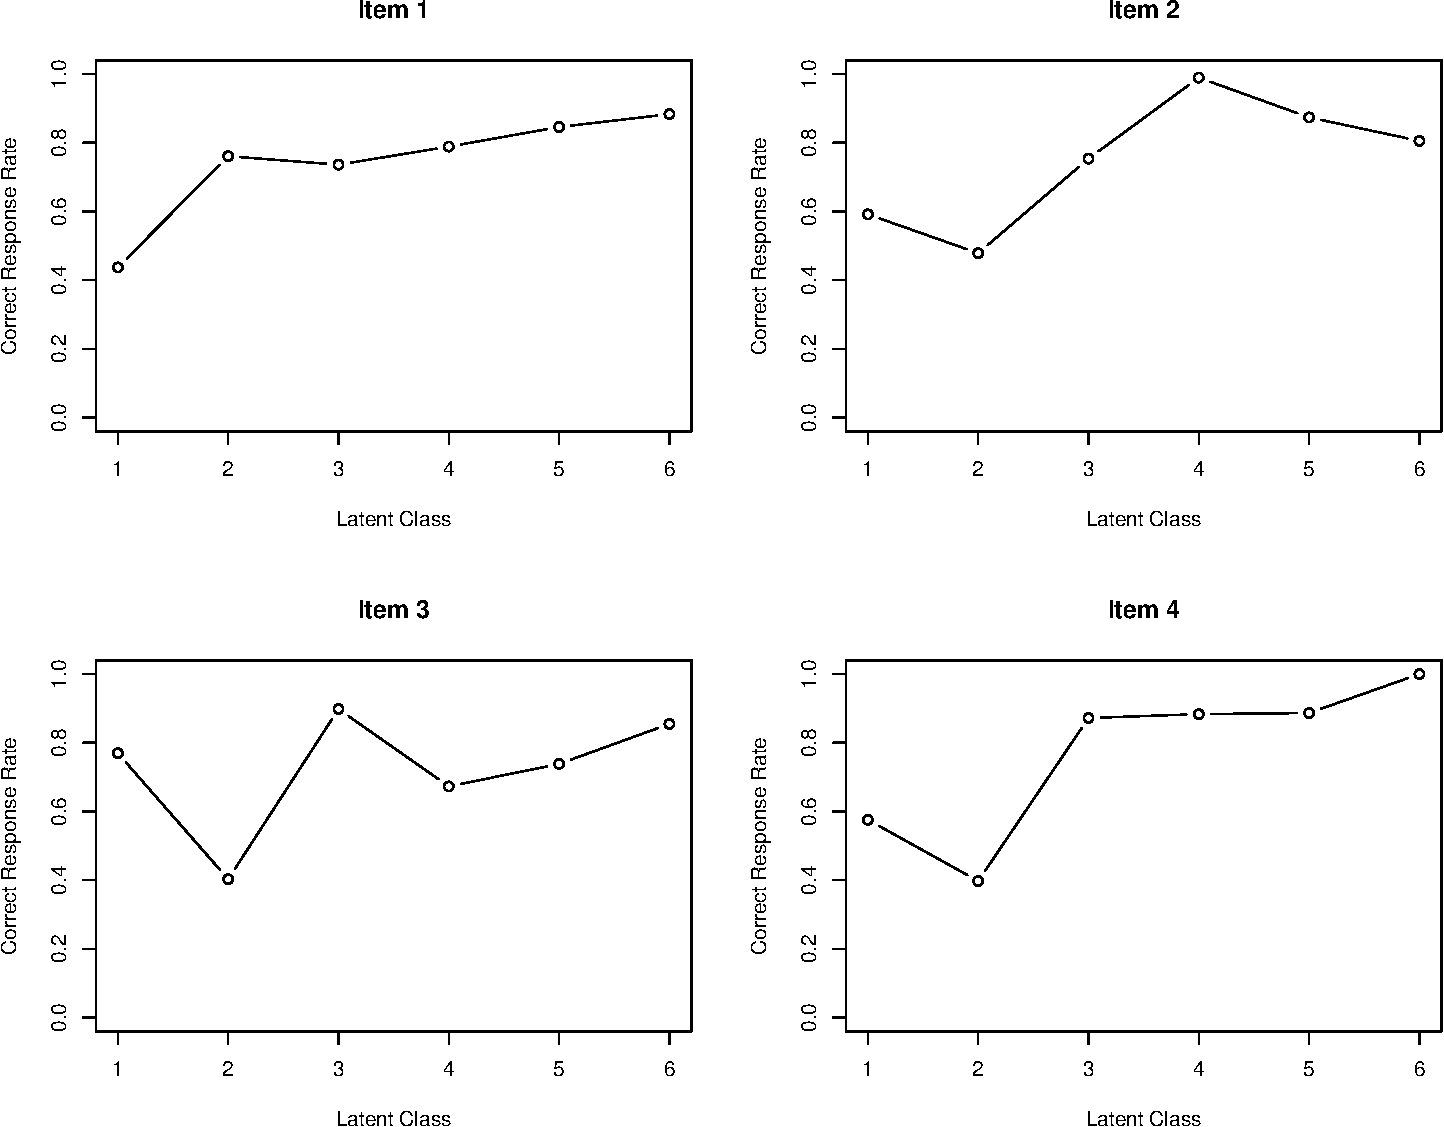
\includegraphics[keepaspectratio]{chap6_LRA_files/figure-pdf/unnamed-chunk-3-1.pdf}}

\subsection{クラスメンバーシッププロファイル}\label{ux30afux30e9ux30b9ux30e1ux30f3ux30d0ux30fcux30b7ux30c3ux30d7ux30d7ux30edux30d5ux30a1ux30a4ux30eb}

\begin{itemize}
\tightlist
\item
  受検者がどのクラスに所属しやすいかの確率を表します
\end{itemize}

\begin{Shaded}
\begin{Highlighting}[]
\NormalTok{result.LCA}\SpecialCharTok{$}\NormalTok{Students }\SpecialCharTok{|\textgreater{}} \FunctionTok{head}\NormalTok{()}
\end{Highlighting}
\end{Shaded}

\begin{verbatim}
           Membership 1 Membership 2 Membership 3 Membership 4 Membership 5
Student001 0.7260153212 0.1695828123 0.0191959227  0.048856576 3.634937e-02
Student002 0.0289874633 0.0254959545 0.8260430686  0.079770428 3.970303e-02
Student003 0.0064609145 0.0694589721 0.7665502806  0.118988645 2.246314e-02
Student004 0.0022440776 0.0037648933 0.1986288018  0.338531342 3.159317e-01
Student005 0.1089417615 0.8873608716 0.0008618367  0.002630128 3.770563e-08
Student006 0.0002507583 0.0002997263 0.0034460370  0.080211142 8.556562e-01
           Membership 6 Estimate
Student001 1.643797e-12        1
Student002 5.150005e-08        3
Student003 1.607805e-02        3
Student004 1.408992e-01        4
Student005 2.053643e-04        2
Student006 6.013617e-02        5
\end{verbatim}

\begin{itemize}
\tightlist
\item
  \texttt{CMP}もプロットできます(しましょう)
\end{itemize}

\begin{Shaded}
\begin{Highlighting}[]
\FunctionTok{plot}\NormalTok{(result.LCA, }\AttributeTok{type =} \StringTok{"CMP"}\NormalTok{, }\AttributeTok{students =} \DecValTok{1}\SpecialCharTok{:}\DecValTok{6}\NormalTok{, }\AttributeTok{nr =} \DecValTok{2}\NormalTok{, }\AttributeTok{nc =} \DecValTok{3}\NormalTok{)}
\end{Highlighting}
\end{Shaded}

\pandocbounded{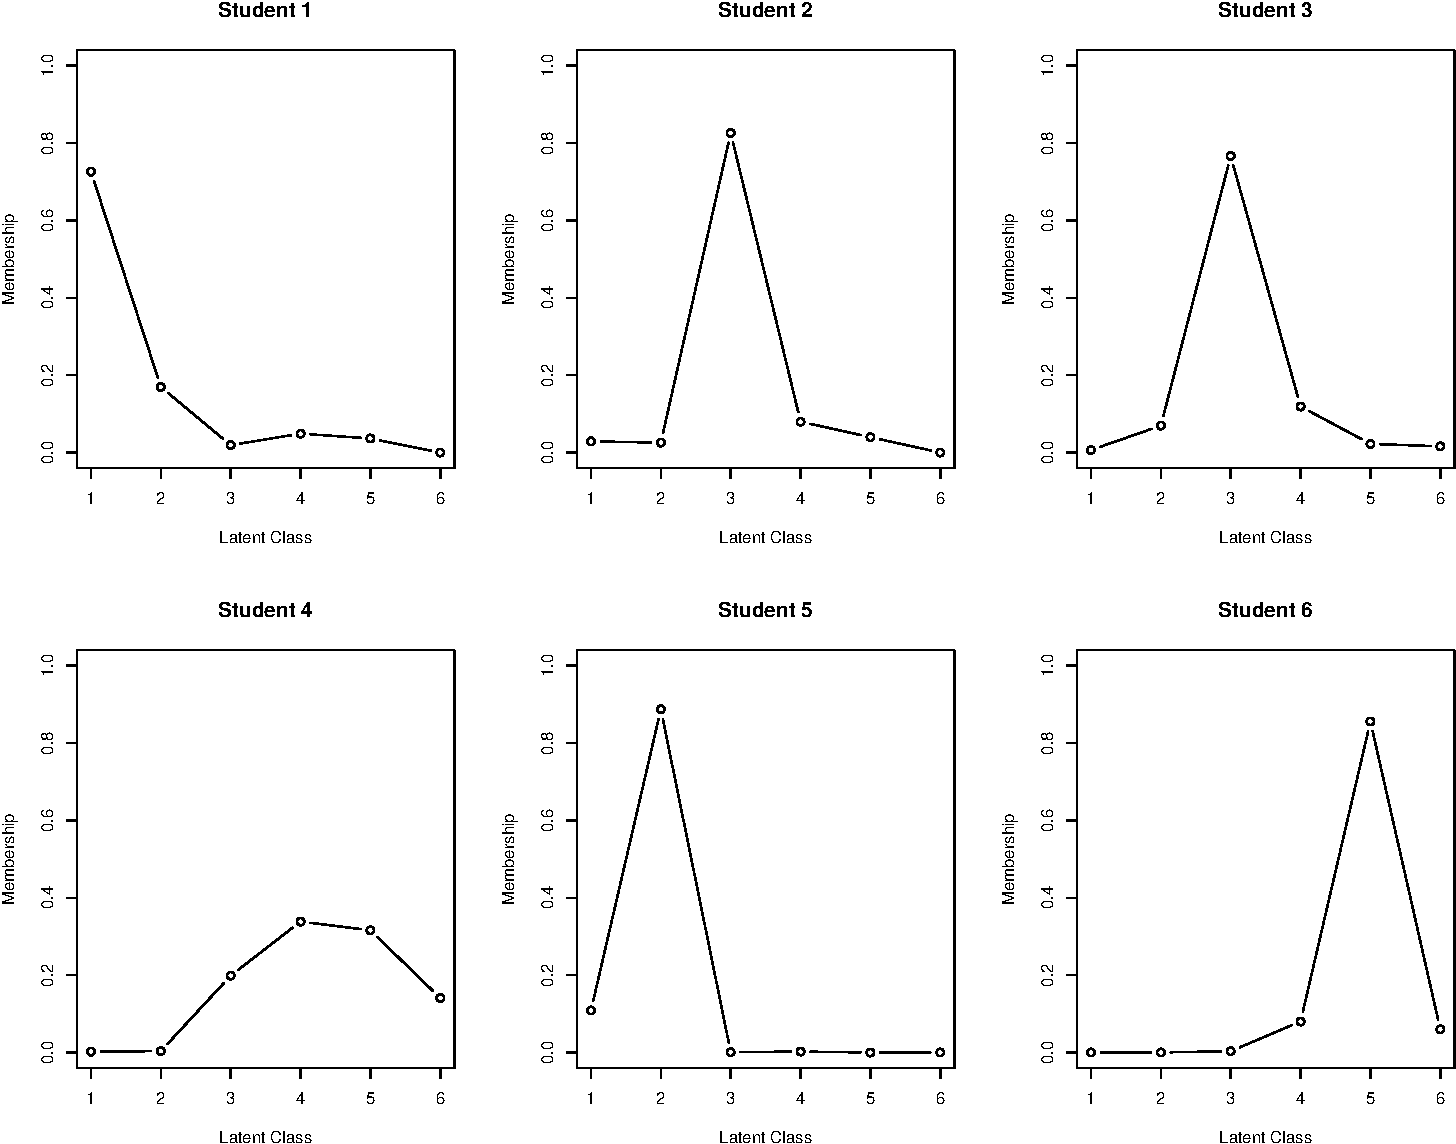
\includegraphics[keepaspectratio]{chap6_LRA_files/figure-pdf/unnamed-chunk-5-1.pdf}}

\section{テスト参照プロファイル}\label{ux30c6ux30b9ux30c8ux53c2ux7167ux30d7ux30edux30d5ux30a1ux30a4ux30eb}

\begin{itemize}
\tightlist
\item
  テストの得点とクラスの分類を可視化します
\end{itemize}

\begin{Shaded}
\begin{Highlighting}[]
\FunctionTok{plot}\NormalTok{(result.LCA, }\AttributeTok{type =} \StringTok{"TRP"}\NormalTok{)}
\end{Highlighting}
\end{Shaded}

\pandocbounded{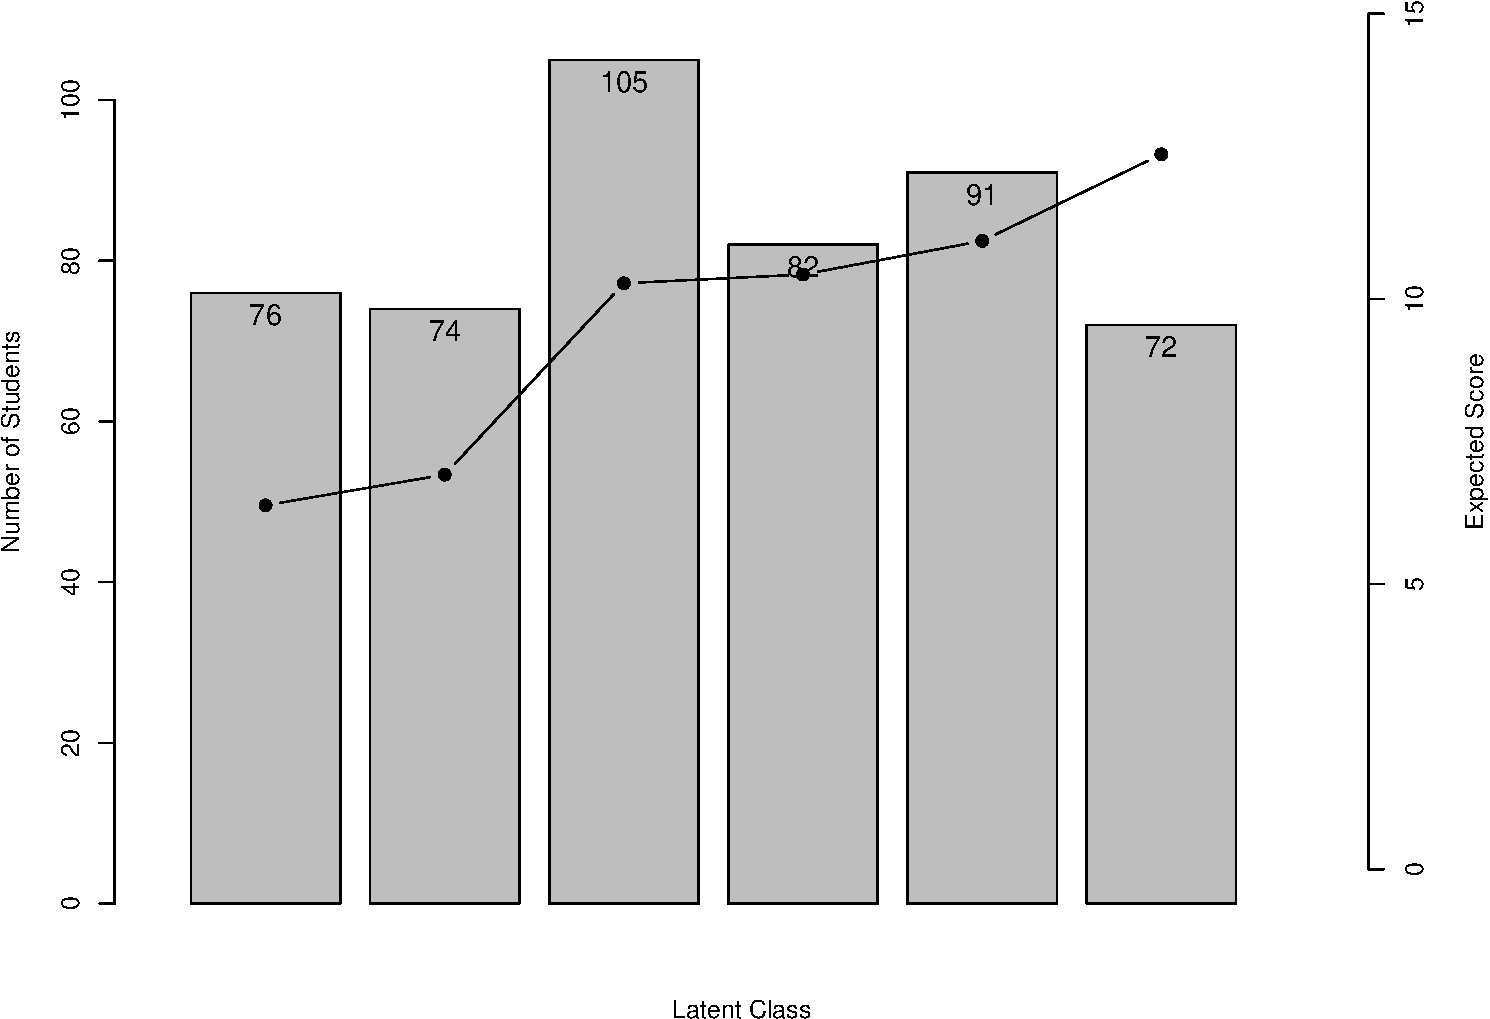
\includegraphics[keepaspectratio]{chap6_LRA_files/figure-pdf/unnamed-chunk-6-1.pdf}}

\section{潜在クラス分布}\label{ux6f5cux5728ux30afux30e9ux30b9ux5206ux5e03}

\begin{itemize}
\tightlist
\item
  クラスの分布をプロットします
\end{itemize}

\begin{Shaded}
\begin{Highlighting}[]
\FunctionTok{plot}\NormalTok{(result.LCA, }\AttributeTok{type =} \StringTok{"LCD"}\NormalTok{)}
\end{Highlighting}
\end{Shaded}

\pandocbounded{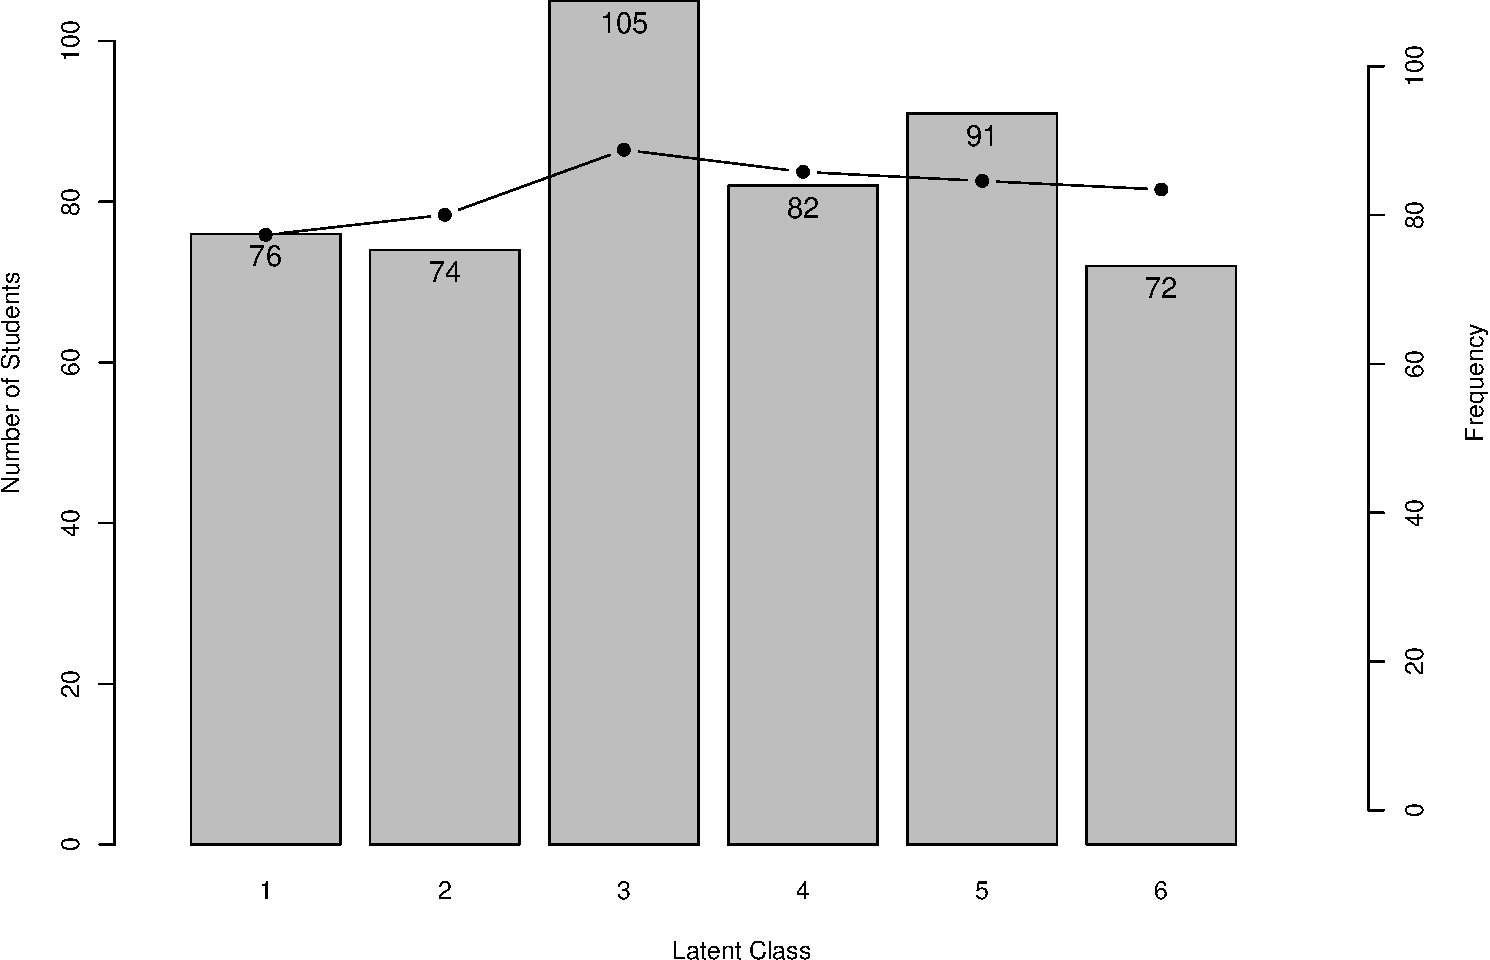
\includegraphics[keepaspectratio]{chap6_LRA_files/figure-pdf/unnamed-chunk-7-1.pdf}}

\section{クラスからランクへ}\label{ux30afux30e9ux30b9ux304bux3089ux30e9ux30f3ux30afux3078}

\subsection{クラスからランクへ}\label{ux30afux30e9ux30b9ux304bux3089ux30e9ux30f3ux30afux3078-1}

\begin{itemize}
\tightlist
\item
  \texttt{LCA}の潜在クラスに序列性を持たせたものが潜在ランク分析(Latent
  Rank Analysis)です

  \begin{itemize}
  \tightlist
  \item
    オプションが\texttt{nrank}になることに注意
  \item
    mic(単調増加オプションmonotonic increasing
    option)を\texttt{TRUE}にすると単調増加の制約を課します
  \end{itemize}
\end{itemize}

\begin{Shaded}
\begin{Highlighting}[]
\NormalTok{result.LRA }\OtherTok{\textless{}{-}} \FunctionTok{LRA}\NormalTok{(dat, }\AttributeTok{nrank =} \DecValTok{6}\NormalTok{, }\AttributeTok{mic =} \ConstantTok{TRUE}\NormalTok{)}
\end{Highlighting}
\end{Shaded}

\begin{verbatim}
Strongly ordinal alignment condition was satisfied.
\end{verbatim}

\begin{Shaded}
\begin{Highlighting}[]
\NormalTok{result.LRA}
\end{Highlighting}
\end{Shaded}

\begin{verbatim}
estimating method is  GTM 

 Monotonic increasing IRP option is TRUE.
Item Reference Profile
         IRP1   IRP2  IRP3  IRP4  IRP5  IRP6
Item01 0.5813 0.6370 0.711 0.780 0.849 0.901
Item02 0.5257 0.6280 0.754 0.837 0.879 0.883
Item03 0.6112 0.6127 0.702 0.768 0.807 0.839
Item04 0.4415 0.5963 0.790 0.889 0.943 0.972
Item05 0.6481 0.7458 0.816 0.829 0.864 0.911
Item06 0.6476 0.7794 0.913 0.937 0.948 0.951
Item07 0.4078 0.5103 0.717 0.841 0.891 0.902
Item08 0.3332 0.4315 0.605 0.702 0.717 0.721
Item09 0.3154 0.3179 0.322 0.334 0.380 0.503
Item10 0.5043 0.5783 0.681 0.724 0.728 0.745
Item11 0.0882 0.0922 0.138 0.274 0.466 0.621
Item12 0.0622 0.0959 0.159 0.253 0.422 0.616
Item13 0.2875 0.4833 0.710 0.766 0.769 0.771
Item14 0.4780 0.6005 0.732 0.844 0.930 0.975
Item15 0.4044 0.5671 0.751 0.824 0.835 0.838

Item Reference Profile Indices
       Alpha      A Beta     B Gamma C
Item01     2 0.0735    1 0.581     0 0
Item02     2 0.1264    1 0.526     0 0
Item03     2 0.0893    1 0.611     0 0
Item04     2 0.1935    1 0.442     0 0
Item05     1 0.0977    1 0.648     0 0
Item06     2 0.1331    1 0.648     0 0
Item07     2 0.2069    2 0.510     0 0
Item08     2 0.1734    2 0.431     0 0
Item09     5 0.1231    6 0.503     0 0
Item10     2 0.1027    1 0.504     0 0
Item11     4 0.1911    5 0.466     0 0
Item12     5 0.1939    5 0.422     0 0
Item13     2 0.2264    2 0.483     0 0
Item14     2 0.1316    1 0.478     0 0
Item15     2 0.1837    2 0.567     0 0

Test Profile
                             Rank 1 Rank 2 Rank 3 Rank 4 Rank 5  Rank 6
Test Reference Profile        6.336  7.676  9.499 10.603 11.426  12.149
Latent Rank Ditribution      97.000 56.000 90.000 89.000 65.000 103.000
Rank Membership Distribution 83.037 77.984 81.981 84.777 84.710  87.511

Item Fit Indices
       model_log_like bench_log_like null_log_like model_Chi_sq null_Chi_sq
Item01       -264.521       -240.190      -283.343       48.662      86.307
Item02       -253.391       -235.436      -278.949       35.909      87.025
Item03       -282.696       -260.906      -293.598       43.580      65.383
Item04       -206.656       -192.072      -265.962       29.169     147.780
Item05       -234.649       -206.537      -247.403       56.224      81.732
Item06       -172.010       -153.940      -198.817       36.141      89.755
Item07       -249.856       -228.379      -298.345       42.954     139.933
Item08       -312.980       -293.225      -338.789       39.510      91.127
Item09       -322.072       -300.492      -327.842       43.159      54.700
Item10       -310.319       -288.198      -319.850       44.240      63.303
Item11       -243.621       -224.085      -299.265       39.071     150.360
Item12       -239.220       -214.797      -293.598       48.847     157.603
Item13       -287.805       -262.031      -328.396       51.549     132.730
Item14       -222.496       -204.953      -273.212       35.086     136.519
Item15       -268.522       -254.764      -302.847       27.518      96.166
       model_df null_df   NFI   RFI   IFI   TLI   CFI RMSEA    AIC    CAIC
Item01    9.233      13 0.436 0.206 0.488 0.243 0.462 0.093 30.197  -8.734
Item02    9.233      13 0.587 0.419 0.657 0.493 0.640 0.076 17.443 -21.487
Item03    9.233      13 0.333 0.062 0.388 0.077 0.344 0.086 25.114 -13.817
Item04    9.233      13 0.803 0.722 0.856 0.792 0.852 0.066 10.704 -28.227
Item05    9.233      13 0.312 0.031 0.352 0.037 0.316 0.101 37.758  -1.173
Item06    9.233      13 0.597 0.433 0.666 0.506 0.649 0.076 17.676 -21.255
Item07    9.233      13 0.693 0.568 0.742 0.626 0.734 0.086 24.489 -14.442
Item08    9.233      13 0.566 0.390 0.630 0.454 0.612 0.081 21.044 -17.886
Item09    9.233      13 0.211 0.000 0.254 0.000 0.186 0.086 24.694 -14.237
Item10    9.233      13 0.301 0.016 0.353 0.020 0.304 0.087 25.775 -13.156
Item11    9.233      13 0.740 0.634 0.789 0.694 0.783 0.080 20.606 -18.325
Item12    9.233      13 0.690 0.564 0.733 0.614 0.726 0.093 30.382  -8.549
Item13    9.233      13 0.612 0.453 0.657 0.502 0.647 0.096 33.084  -5.847
Item14    9.233      13 0.743 0.638 0.797 0.705 0.791 0.075 16.621 -22.310
Item15    9.233      13 0.714 0.597 0.790 0.690 0.780 0.063  9.052 -29.879
           BIC
Item01  -8.716
Item02 -21.469
Item03 -13.798
Item04 -28.209
Item05  -1.154
Item06 -21.236
Item07 -14.424
Item08 -17.868
Item09 -14.219
Item10 -13.137
Item11 -18.307
Item12  -8.531
Item13  -5.829
Item14 -22.292
Item15 -29.860

Model Fit Indices
Number of Latent rank: 6
Number of EM cycle: 13 
                   value
model_log_like -3870.815
bench_log_like -3560.005
null_log_like  -4350.217
model_Chi_sq     621.620
null_Chi_sq     1580.424
model_df         138.491
null_df          195.000
NFI                0.607
RFI                0.446
IFI                0.665
TLI                0.509
CFI                0.651
RMSEA              0.084
AIC              344.638
CAIC            -239.324
BIC             -239.047
\end{verbatim}

\subsection{項目参照プロファイル}\label{ux9805ux76eeux53c2ux7167ux30d7ux30edux30d5ux30a1ux30a4ux30eb-1}

\begin{itemize}
\tightlist
\item
  項目参照プロファイル(Item Reference
  Profile)は,項目と潜在クラスの関係を表しています

  \begin{itemize}
  \tightlist
  \item
    項目ごと・クラスごとの正答率を返します
  \end{itemize}
\end{itemize}

\begin{Shaded}
\begin{Highlighting}[]
\NormalTok{result.LRA}\SpecialCharTok{$}\NormalTok{IRP}
\end{Highlighting}
\end{Shaded}

\begin{verbatim}
             IRP1       IRP2      IRP3      IRP4      IRP5      IRP6
Item01 0.58134579 0.63703070 0.7105624 0.7799727 0.8488455 0.9005402
Item02 0.52566747 0.62802753 0.7544298 0.8369062 0.8793933 0.8828570
Item03 0.61116426 0.61266166 0.7019998 0.7679128 0.8071646 0.8391724
Item04 0.44152626 0.59634830 0.7898921 0.8885698 0.9427475 0.9724996
Item05 0.64810054 0.74581736 0.8158043 0.8292063 0.8635791 0.9113865
Item06 0.64762411 0.77943717 0.9125559 0.9366776 0.9476421 0.9507004
Item07 0.40777315 0.51032060 0.7172665 0.8414449 0.8909572 0.9019490
Item08 0.33320297 0.43146180 0.6048313 0.7022176 0.7165168 0.7207851
Item09 0.31536164 0.31793335 0.3215534 0.3337615 0.3799428 0.5030880
Item10 0.50433135 0.57829599 0.6809487 0.7244593 0.7284557 0.7447081
Item11 0.08816694 0.09217932 0.1376948 0.2744389 0.4655814 0.6209129
Item12 0.06219226 0.09589473 0.1590574 0.2528391 0.4223461 0.6162779
Item13 0.28748283 0.48325773 0.7096872 0.7658707 0.7689499 0.7711838
Item14 0.47797956 0.60051446 0.7321160 0.8442909 0.9295404 0.9747505
Item15 0.40437730 0.56707341 0.7507473 0.8243016 0.8346267 0.8378010
\end{verbatim}

\begin{Shaded}
\begin{Highlighting}[]
\FunctionTok{plot}\NormalTok{(result.LRA, }\AttributeTok{type =} \StringTok{"IRP"}\NormalTok{, }\AttributeTok{items =} \DecValTok{1}\SpecialCharTok{:}\DecValTok{4}\NormalTok{, }\AttributeTok{nr =} \DecValTok{2}\NormalTok{, }\AttributeTok{nc =} \DecValTok{2}\NormalTok{)}
\end{Highlighting}
\end{Shaded}

\pandocbounded{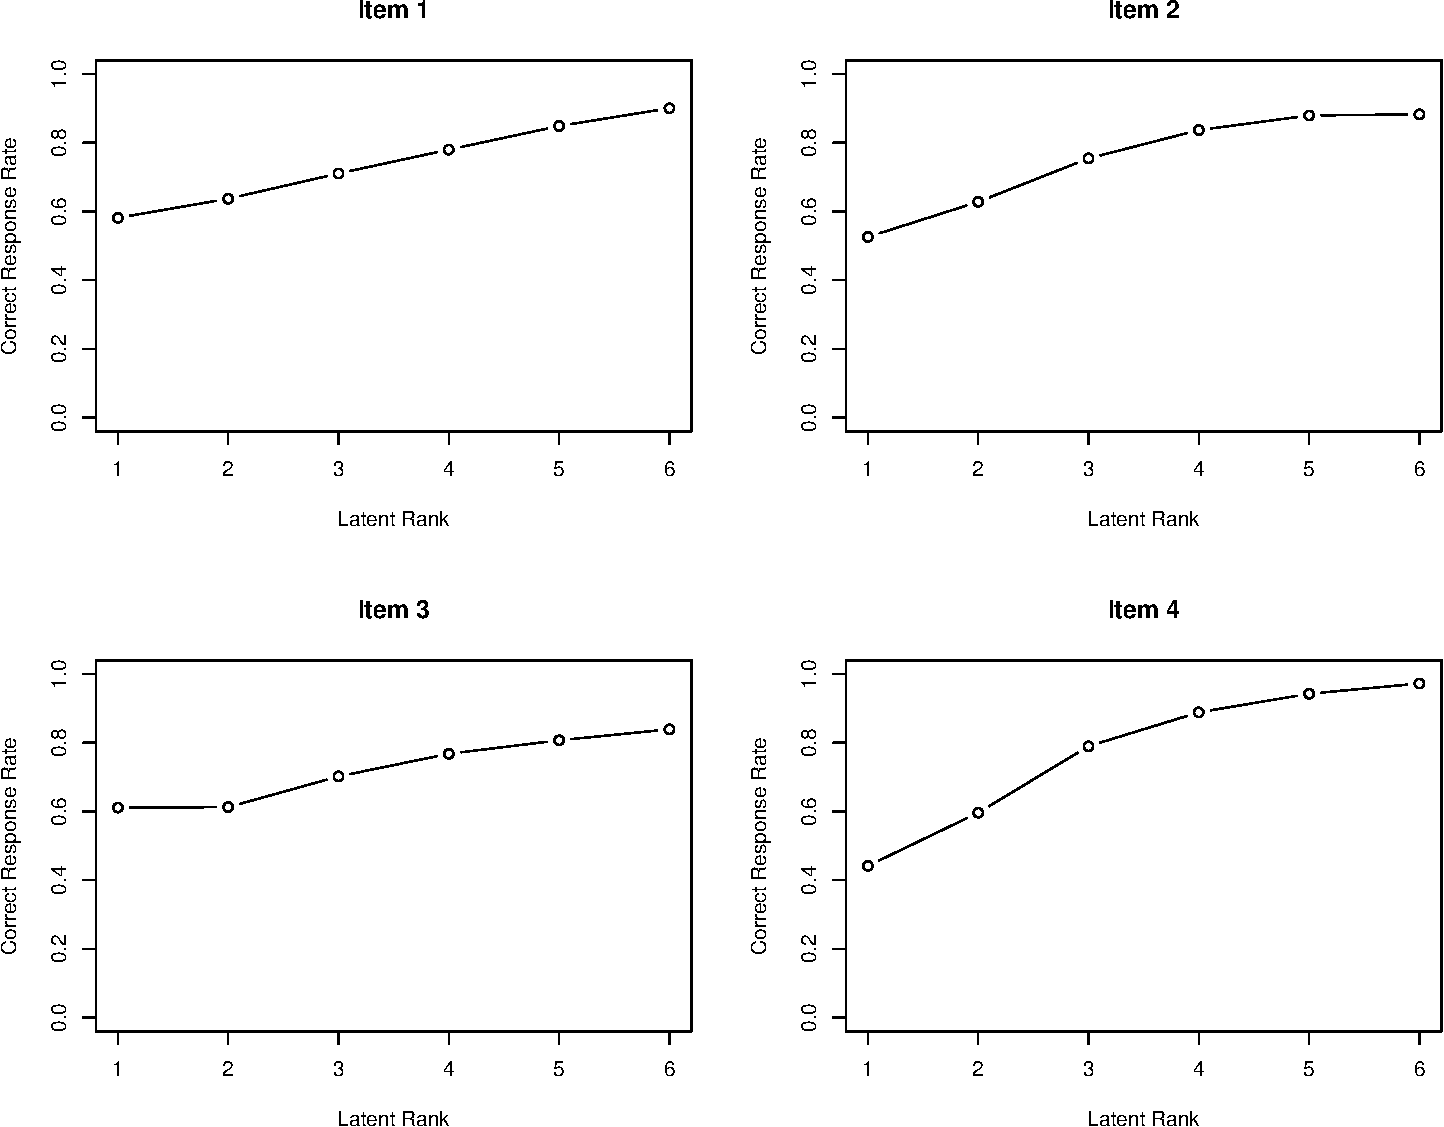
\includegraphics[keepaspectratio]{chap6_LRA_files/figure-pdf/unnamed-chunk-10-1.pdf}}

\subsection{ランクメンバーシッププロファイル}\label{ux30e9ux30f3ux30afux30e1ux30f3ux30d0ux30fcux30b7ux30c3ux30d7ux30d7ux30edux30d5ux30a1ux30a4ux30eb}

\begin{itemize}
\tightlist
\item
  受検者がどのクラスに所属しやすいかの確率を表します

  \begin{itemize}
  \tightlist
  \item
    \texttt{Rank-Up\ Odds}や\texttt{Rank-Down\ Odds}が表示されています
  \item
    上のランクへの上がりやすさ,下のランクへの落ちやすさの指標です
  \end{itemize}
\end{itemize}

\begin{Shaded}
\begin{Highlighting}[]
\NormalTok{result.LRA}\SpecialCharTok{$}\NormalTok{Students }\SpecialCharTok{|\textgreater{}} \FunctionTok{head}\NormalTok{()}
\end{Highlighting}
\end{Shaded}

\begin{verbatim}
           Membership 1 Membership 2 Membership 3 Membership 4 Membership 5
Student001 0.2649442154  0.401777727   0.25199194  0.069833913  0.010587063
Student002 0.0320802124  0.165197013   0.47017520  0.262193334  0.061017540
Student003 0.0256087173  0.143643145   0.36931821  0.263791224  0.137653365
Student004 0.0019080554  0.015030869   0.09499327  0.201622664  0.343207280
Student005 0.5745639230  0.379140089   0.03754276  0.006239969  0.001910557
Student006 0.0003651887  0.003620252   0.04607054  0.202440568  0.398545000
           Membership 6 Estimate Rank-Up Odds Rank-Down Odds
Student001 0.0008651363        2    0.6271924      0.6594298
Student002 0.0093367003        3    0.5576503      0.3513520
Student003 0.0599853347        3    0.7142654      0.3889414
Student004 0.3432378584        6           NA      0.9999109
Student005 0.0006027066        1    0.6598745             NA
Student006 0.3489584503        5    0.8755811      0.5079491
\end{verbatim}

\subsection{ランクメンバーシッププロファイル}\label{ux30e9ux30f3ux30afux30e1ux30f3ux30d0ux30fcux30b7ux30c3ux30d7ux30d7ux30edux30d5ux30a1ux30a4ux30eb-1}

\begin{itemize}
\tightlist
\item
  \texttt{CMP}のランク版,\texttt{RMP}もプロットできます(しましょう)
\end{itemize}

\begin{Shaded}
\begin{Highlighting}[]
\FunctionTok{plot}\NormalTok{(result.LRA, }\AttributeTok{type =} \StringTok{"RMP"}\NormalTok{, }\AttributeTok{students =} \DecValTok{1}\SpecialCharTok{:}\DecValTok{6}\NormalTok{, }\AttributeTok{nr =} \DecValTok{2}\NormalTok{, }\AttributeTok{nc =} \DecValTok{3}\NormalTok{)}
\end{Highlighting}
\end{Shaded}

\pandocbounded{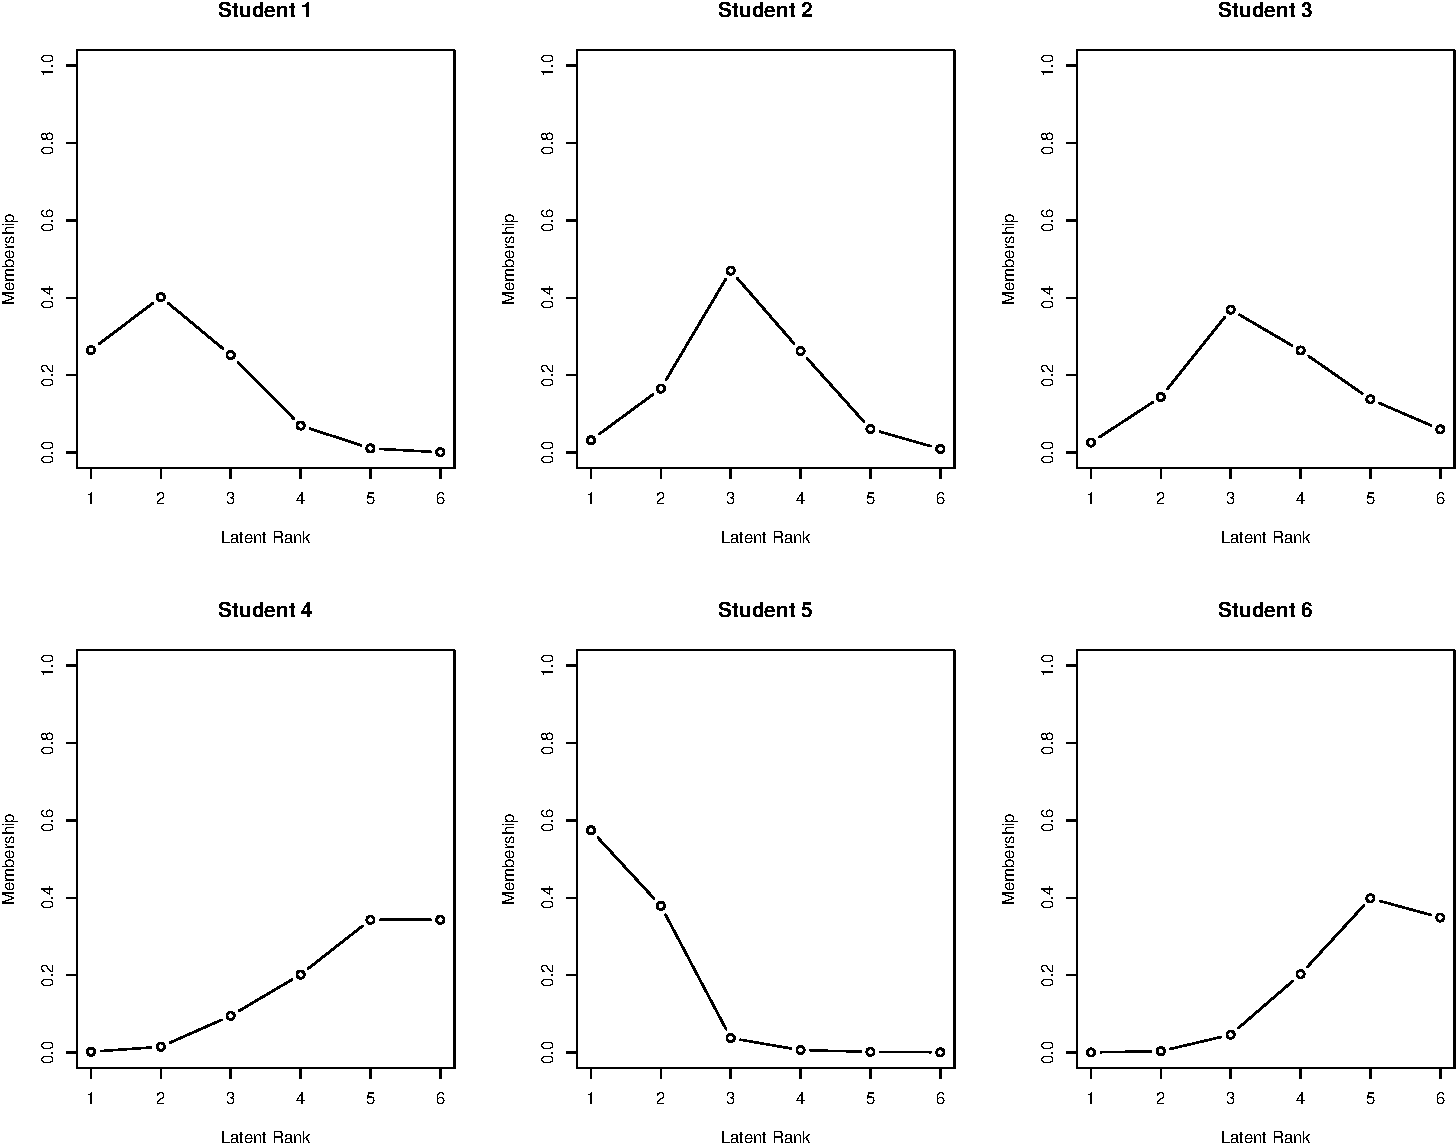
\includegraphics[keepaspectratio]{chap6_LRA_files/figure-pdf/unnamed-chunk-12-1.pdf}}

\subsection{テスト参照プロファイル}\label{ux30c6ux30b9ux30c8ux53c2ux7167ux30d7ux30edux30d5ux30a1ux30a4ux30eb-1}

\begin{itemize}
\tightlist
\item
  テストの得点とクラスの分類を可視化します
\end{itemize}

\begin{Shaded}
\begin{Highlighting}[]
\FunctionTok{plot}\NormalTok{(result.LRA, }\AttributeTok{type =} \StringTok{"TRP"}\NormalTok{)}
\end{Highlighting}
\end{Shaded}

\pandocbounded{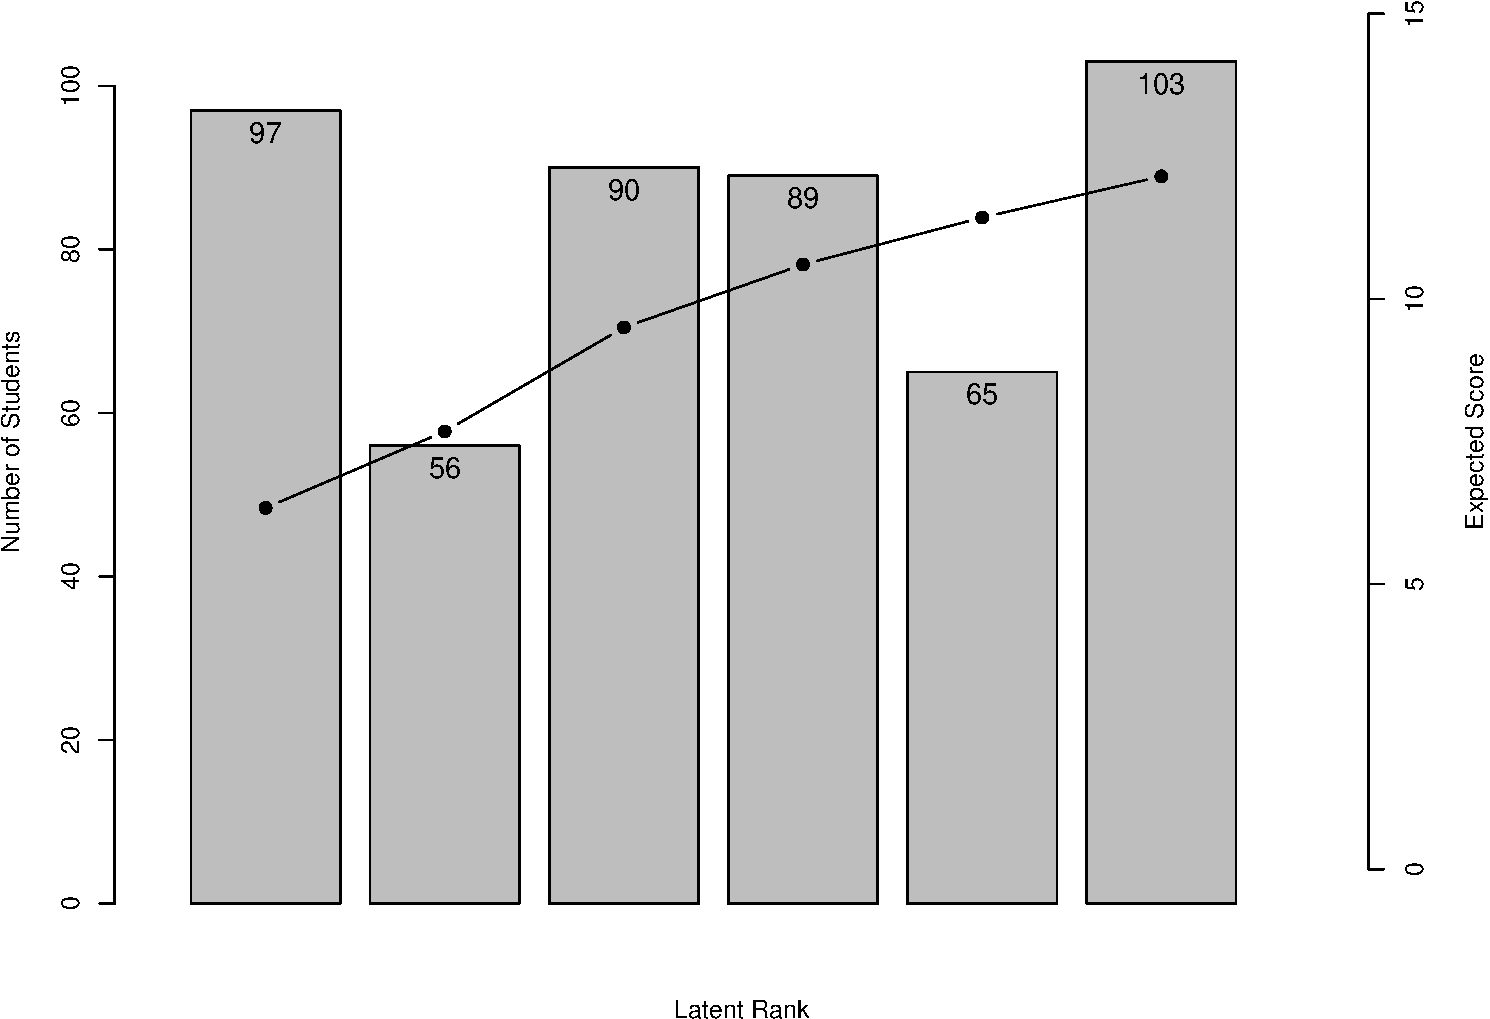
\includegraphics[keepaspectratio]{chap6_LRA_files/figure-pdf/unnamed-chunk-13-1.pdf}}

\subsection{潜在ランク分布}\label{ux6f5cux5728ux30e9ux30f3ux30afux5206ux5e03}

\begin{itemize}
\tightlist
\item
  クラスの分布をプロットします
\end{itemize}

\begin{Shaded}
\begin{Highlighting}[]
\FunctionTok{plot}\NormalTok{(result.LRA, }\AttributeTok{type =} \StringTok{"LRD"}\NormalTok{)}
\end{Highlighting}
\end{Shaded}

\pandocbounded{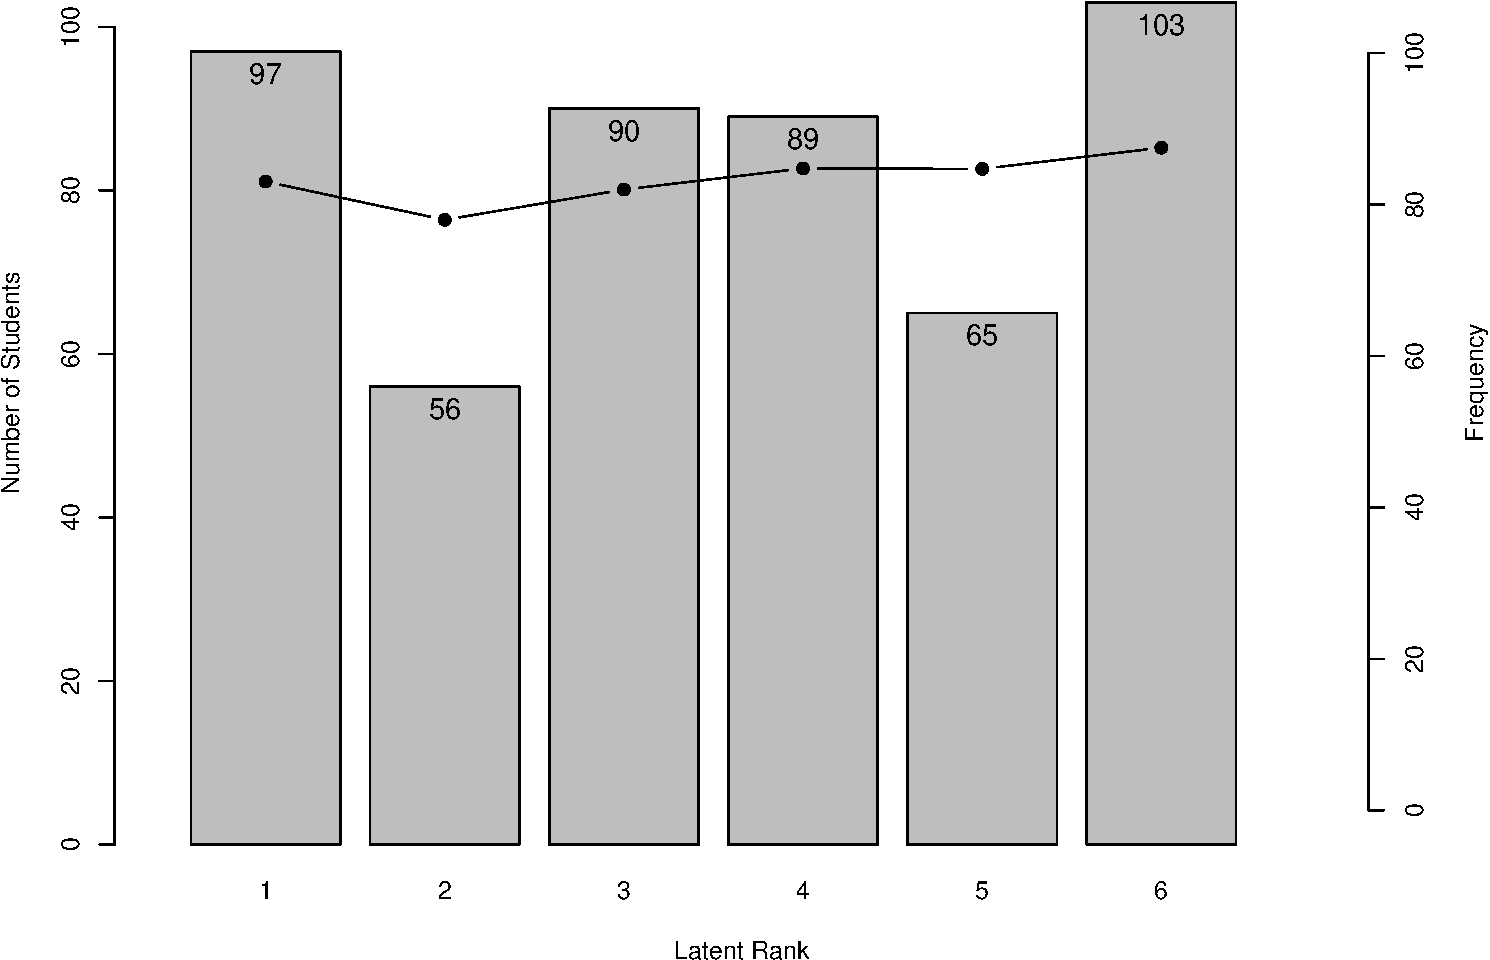
\includegraphics[keepaspectratio]{chap6_LRA_files/figure-pdf/unnamed-chunk-14-1.pdf}}

\subsection{その他の出力}\label{ux305dux306eux4ed6ux306eux51faux529b}

\begin{itemize}
\tightlist
\item
  \texttt{IRP\ index}を表示することができます

  \begin{itemize}
  \tightlist
  \item
  \end{itemize}
\end{itemize}

\begin{Shaded}
\begin{Highlighting}[]
\NormalTok{result.LRA}\SpecialCharTok{$}\NormalTok{IRPIndex}
\end{Highlighting}
\end{Shaded}

\begin{verbatim}
       Alpha          A Beta         B Gamma C
Item01     2 0.07353170    1 0.5813458     0 0
Item02     2 0.12640232    1 0.5256675     0 0
Item03     2 0.08933814    1 0.6111643     0 0
Item04     2 0.19354385    1 0.4415263     0 0
Item05     1 0.09771682    1 0.6481005     0 0
Item06     2 0.13311875    1 0.6476241     0 0
Item07     2 0.20694595    2 0.5103206     0 0
Item08     2 0.17336955    2 0.4314618     0 0
Item09     5 0.12314521    6 0.5030880     0 0
Item10     2 0.10265274    1 0.5043314     0 0
Item11     4 0.19114249    5 0.4655814     0 0
Item12     5 0.19393177    5 0.4223461     0 0
Item13     2 0.22642950    2 0.4832577     0 0
Item14     2 0.13160157    1 0.4779796     0 0
Item15     2 0.18367392    2 0.5670734     0 0
\end{verbatim}

\section{2種類の推定法があります}\label{ux7a2eux985eux306eux63a8ux5b9aux6cd5ux304cux3042ux308aux307eux3059}




\end{document}
